\documentclass[12pt]{report}
% Packages
\usepackage[utf8]{vietnam} % Enable vi language compile 
\usepackage[a4paper, top=3cm, right=2cm, bottom=3.5cm, left=3.5cm]{geometry} % Define document
\usepackage{graphicx} % Display picture
\usepackage{subcaption} % Use subfigure in \begin ({minipage} used to be)
\usepackage{tabularx} % Support advance table
\usepackage{ltablex} % Table into next page
\usepackage{makecell} % Create header of table in {tabularx}
\usepackage{tabto} % Support \tab command to tab text 0.5cm (similar to  \hspace{5mm})
\usepackage{amssymb} % Use \checkmark to represent V mark
\usepackage{times} % Times font
\usepackage{lipsum} % Support create dot command
\usepackage{float} % Able to use H
\usepackage{listings}
\usepackage{xcolor}
\usepackage{hyperref}
\usepackage{nameref}
\usepackage{tocloft}
\usepackage{tikz}
\usetikzlibrary{calc}
\usetikzlibrary{decorations.pathmorphing}
\usepackage[backend=bibtex,
style=numeric,
bibencoding=ascii,
sorting=none
]{biblatex}
\addbibresource{bibliography.bib}

% ----------------------------------------
\linespread{1.5}
\keepXColumns % Keep X column in ltablex to avoid \item missing error
\definecolor{codegreen}{rgb}{0,0.6,0}
\definecolor{codegray}{rgb}{0.5,0.5,0.5}
\definecolor{codepurple}{rgb}{0.58,0,0.82}
\definecolor{backcolour}{rgb}{0.95,0.95,0.92}
\setcounter{secnumdepth}{3}

\lstdefinestyle{mystyle}{
    backgroundcolor=\color{backcolour},   
    commentstyle=\color{codegreen},
    keywordstyle=\color{magenta},
    numberstyle=\tiny\color{codegray},
    stringstyle=\color{codepurple},
    basicstyle=\ttfamily\footnotesize,
    breakatwhitespace=false,         
    breaklines=true,                 
    captionpos=b,                    
    keepspaces=true,                 
    numbers=left,                    
    numbersep=5pt,                  
    showspaces=false,                
    showstringspaces=false,
    showtabs=false,                  
    tabsize=2
}
% % Macros that change \paragraph behavior what add space below the paragraph without new line dirty trick
% \makeatletter
% \renewcommand\paragraph{\@startsection{paragraph}{4}{\z@}%
%   {-3ex plus -1ex minus -1ex}% change as needed
%   {1.5ex plus .1ex minus .1ex}% change as needed
%   {\bfseries}} % change as needed
% \makeatother
\newcommand{\myparagraph}[1]{\paragraph{#1}\mbox{}\\} % Add space below \paragraph
\renewcommand\tabularxcolumn[1]{m{#1}} % Verticle center text in cell
\renewcommand{\theadfont}{\bfseries} % Set \thead to Bold text % Set \thead to Bold text
\newcommand{\newlinecontenttable}{\newline[1ex]} % Add space under \newline % Add space \newline
\newcommand{\xmark}{$\times$} % Use new command \xmark to represent X mark
\makeatletter

\newcommand*\dotcolumnfill{%
    \par
    \null
    \vskip -\ht\strutbox
    \xleaders \hb@xt@ \hsize {%
        \strut \cleaders \hb@xt@ .44em{\hss.\hss}\hfill
    }\vfill
}

\makeatother % Use dot spread

\renewcommand*\listfigurename{Danh sách hình}

\newcommand{\applicationname}{Owlens\:}

\begin{document}

\pagenumbering{gobble}
\newgeometry{a4paper, bottom=2cm}
\begin{center}
    \centering

    \textbf{\textsf{\large TRƯỜNG ĐẠI HỌC KHOA HỌC TỰ NHIÊN }} 

    % \vspace{0.5cm}

    \textbf{\textsf{\large KHOA CÔNG NGHỆ THÔNG TIN }}
    
    % \vspace{0.5cm}

    \textbf{\textsf{\large BỘ MÔN CÔNG NGHỆ PHẦN MỀM }}
    
    \vspace{2.5cm}
    
    \textbf{\large PHẠM GIA HUY - 18127108}
    
    \vspace{0.25cm}

    \textbf{\large NGUYỄN QUÝ THANH - 18127210}
    
    \vspace{2.5cm}

    \textbf{\textsf{\LARGE HỆ THỐNG TỰ ĐỘNG TÌM KIẾM LỖI BẢO MẬT ỨNG DỤNG WEB DỰA TRÊN NỀN TẢNG ZAP }}
    
    \vspace{2cm}
    
    \textbf{\large KHÓA LUẬN TỐT NGHIỆP CỬ NHÂN CNTT }

    \vspace{2cm}

    \large GIÁO VIÊN HƯỚNG DẪN

    \vspace{0.25cm}

    \textbf{\textsf{\large TS. Ngô Huy Biên }}
    
    \vspace{2.5cm}
    
    \textbf{\large TP. HCM, 2023 }    
\end{center}
\newpage
\begin{center}
    \begin{tikzpicture}[overlay,remember picture]
        \draw [line width=3pt]
               ($ (current page.north west) + (1.5cm,-2.0cm) $)
            rectangle
            ($ (current page.south east) + (-1.5cm,1.8cm) $);
        \end{tikzpicture}
        
    \textbf{\large TRƯỜNG ĐẠI HỌC KHOA HỌC TỰ NHIÊN} 
    
    \textbf{\large KHOA CÔNG NGHỆ THÔNG TIN}
    
    \vspace{2cm}
    
    \textbf{\large PHẠM GIA HUY - 18127108}
    
    \textbf{\large NGUYỄN QUÝ THANH - 18127210}
    
    \vspace{2cm}
    
    \textbf{\large HỆ THỐNG TỰ ĐỘNG TÌM KIẾM LỖI BẢO MẬT ỨNG DỤNG WEB DỰA TRÊN NỀN TẢNG ZAP }
    
    \vspace{2cm}
    
    \textbf{\large KHÓA LUẬN TỐT NGHIỆP CỬ NHÂN CNTT}

    \textbf{\large CHƯƠNG TRÌNH CHẤT LƯỢNG CAO}
    
    \vspace{2cm}
    
    \textbf{\large GIÁO VIÊN HƯỚNG DẪN}
    
    \textbf{\large TS. NGÔ HUY BIÊN}
    
    \vspace{6.5cm}
    
    \textbf{\large TP. HCM, 2023 }    
\end{center}


    

    
\restoregeometry
% \newpage
\phantomsection
\addcontentsline{toc}{chapter}{NHẬN XÉT CỦA GIÁO VIÊN HƯỚNG DẪN}
\begin{center}
\textbf{\Large NHẬN XÉT CỦA GIÁO VIÊN HƯỚNG DẪN }
\vspace{1cm}
\dotcolumnfill
\end{center}

\hspace{7cm}TpHCM, ngày ..... tháng ..... năm ....

\hspace{8.5cm}Giáo viên hướng dẫn

\hspace{8.5cm}[Ký và ghi rõ họ tên]
% \newpage
\begin{center}
\textbf{\Large NHẬN XÉT CỦA GIÁO VIÊN PHẢN BIỆN }
\vspace{1cm}
\dotcolumnfill
\end{center}

\pagenumbering{roman}
\newpage
\begin{center}
\textbf{\Large LỜI CẢM ƠN }
\vspace{1cm}
\end{center}

Lời đầu tiên, nhóm chúng em xin gửi lời cảm ơn vô cùng chân thành đến Thầy - Tiến sĩ Ngô Huy Biên đã tạo điều kiện cho nhóm có cơ hội để thực hiện khóa luận này. Trong suốt thời gian thực hiện khóa luận, nhóm đã gặp nhiều khó khăn và thầy là người đã hướng dẫn và giúp đỡ nhóm rất nhiều. Thầy đã đưa ra các lời khuyên đáng giá và hỗ trợ nhóm khi gặp vấn đề, giúp cho nhóm có thể vượt qua khó khăn và có được các định hướng tốt hơn. Nhờ sự hỗ trợ nhiệt của thầy trong suốt thời gian qua, nhóm mới có thể hoàn thành tốt khóa luận. Một lần nữa, nhóm em xin gửi đến thầy lời cảm ơn sâu sắc nhất!

Tiếp theo, nhóm chúng em xin được gửi lời tri ân đến quý Thầy Cô trong khoa Công nghệ Thông tin của trường đại học Khoa Học Tự Nhiên đã tận tình giảng dạy và giúp nhóm chúng em trang bị các kiến thức cần thiết để có thể thực hiện khóa luận. Các kiến thức của thầy cô sẽ là những kinh nghiệm quý giá giúp nhóm em trong cả con đường về sau.

Nhóm em xin cảm ơn khoa Công nghệ Thông Tin và trường Đại học Khoa học tự nhiên, xin cảm ơn các thầy cô trong bộ phận công tác sinh viên và ban quản trị nhà trường. Nhờ những lần thông tin giải đáp thắc mắc, hỗ trợ và thông báo của thầy cô giúp nhóm em có điều kiện thuận lợi để hoàn thoàn khóa luận.

Trong quá trình thực hiện khóa luận, nhóm em đã cố gắng hoàn thành khóa luận bằng tất cả khả năng cho phép. Dù vậy, khó có thể tránh khỏi các lỗi lầm và thiết sót. Nên nhóm em hi vọng thầy cô sẽ thông cảm, chỉ bảo và đưa ra những phản hồi để giúp khóa luận trở nên hoàn thiện hơn.

Cuối cùng, nhóm em xin mong chúc các thầy cô sẽ có nhiều sức khỏe và tinh thần để hoàn thành tốt công tác giảng dạy, và gặp nhiều thành công trong cuộc sống.

\vspace{2cm}

\hspace{6cm}Thành phố Hồ Chí Minh, ngày ..... tháng ..... năm ....

% THESIS PROPOSAL
\begin{titlepage}
    \centering
    \begin{figure}
        \begin{subfigure}[c][][t]{0.2\textwidth}
            % Manual resize img at the final release with the purpose remove [scale] property 
            
\includegraphics[width=\textwidth]{images/logo.jpg}
        \end{subfigure}
        \hspace{40pt}
        \begin{subfigure}[c][][t]{0.69\textwidth}
            \centering
            \textbf{TRƯỜNG ĐẠI HỌC KHOA HỌC TỰ NHIÊN\\
                    CHƯƠNG TRÌNH CHẤT LƯỢNG CAO}
        \end{subfigure}
    \end{figure}
    
    \vspace*{20pt}

    \textbf{\large ĐỀ CƯƠNG KHÓA LUẬN TỐT NGHIỆP}\\
    
    \vspace{10pt}
    
    \textbf{\LARGE HỆ THỐNG TỰ ĐỘNG TÌM KIẾM LỖI BẢO MẬT ỨNG DỤNG WEB DỰA TRÊN NỀN TẢNG ZAP }

    \vspace{10pt}

    \textbf{\textsl{\large (AUTOMATED WEB APPLICATION SECURITY SCANNER BASED ON ZAP)}}
\end{titlepage}
\newpage

\section{THÔNG TIN CHUNG}

\paragraph{Người hướng dẫn}
\tab - TS. Ngô Huy Biên (Khoa Công nghệ Thông tin)    

\paragraph{[Nhóm] Sinh viên thực hiện:}
\begin{enumerate}
    \item Phạm Gia Huy (MSSV: 18127018)
    \item Nguyễn Quý Thanh (MSSV: 18127210)
\end{enumerate}

\paragraph{Loại đề tài:}
Ứng dụng

\paragraph{Thời gian thực hiện:}
Từ \textsl{04/2023} đến \textsl{08/2023}

% \newpage
\section*{2  NỘI DUNG THỰC HIỆN}

\subsection{Giới thiệu đề tài}
\tab Khi phát triển phần mềm hay ứng dụng, bước cần thiết nhất và không thể thiếu
trước khi triển khai sản phẩm vào thực tế là kiểm thử. Có rất nhiều vấn đề ta cần
quan tâm khi tiến hành kiểm thử một ứng dụng, vấn đề bảo mật là một trong số đó. Bảo mật
của một ứng dụng là một vấn đề quan trọng thấy rõ mà nhiều ứng dụng bỏ qua hoặc chưa xử lý, phát hiện
được triệt để các lỗi này. Vì vậy, với tâm lý này làm cho sự xuất hiện của các người dùng tiêu cực và
nhà phát triển tiêu cực ngày càng nhiều và phát triển nhanh chóng, hậu quả gây ra là khôn lường.
Do đó, nhóm sinh viên muốn tạo ra một hệ thống kiểm thử bảo mật trực tuyến, giúp cho việc kiểm thử diễn ra dễ dàng,
nhanh gọn, trực quan hơn. Tên là \applicationname - Hệ thống tự động tìm kiếm lỗi bảo mật ứng dụng web dựa trên nền tảng ZAP (Automated web application security scanner based on ZAP)
\subsection{Mục tiêu đề tài}
\paragraph{Thiết kế, xây dựng, kiểm thử và triển khai hệ thống}
\tab Nhóm sinh viên thực hiện mong muốn hoàn thành tối thiểu 80\% - 95\% các chức năng đề ra ban đầu. Các chức năng và mục tiêu chính bao gồm:
\begin{itemize}
    \item Đăng ký / Đăng nhập tài khoản cá nhân để lưu trữ thông tin trong quá trình sử dụng.
    \item Xác thực, cập nhật, bảo mật thông tin tài khoản và lịch sử sử dụng.
    \item Quét ứng dụng web qua URL hoặc IP bằng các loại quét, kịch bản nền tảng ZAP có hỗ trợ.
    \item Hỗ trợ cấu hình các phiên quét ánh xạ với nền tảng ZAP.
    \item Hỗ trợ các loại quét khác như Nmap Port, OpenVas Network Vulnerability và Sslyze TLS/SSL Security.
    \item Quản lý thông tin các URL hoặc IP dùng để quét và các thông tin liên quan.
    \item Giao diện quá trình quét trực quan.
    \item Quản lý các kết quả của các phiên quét.
    \item Giao diện kết quả sau khi quét xong đầy đủ thông tin.
    \item Gửi kết quả trạng thái quét, báo cáo rút gọn qua mail.
    \item Xuất báo cáo với định dạng pdf, xml.
    \item Lịch sử quản lý thông tin các lần quét trước và thông tin kế quả quét.
    \item Các thông tin giới thiệu website của ứng dụng; Trang FAQ; Thông tin liên hệ và hỗ trợ.
    \item Tài liệu đồ án đề tài hoàn thành chi tiết, đầy đủ và bài bản.
\end{itemize}
\paragraph{Tài liệu}
\begin{itemize}
    \item Viết 20 trang Đề cương chi tiết theo mẫu của khoa.
    \item Viết 100 trang khóa luận.
    \item Tài liệu kĩ thuật.
    \begin{itemize}
        \item Hướng dẫn cài đặt công cụ và biên dịch mã nguồn (khoảng 20 trang).
        \item Hướng dẫn triển khai hệ thống (khoảng 30 trang).
        \item Hướng dẫn sử dụng hệ thống (khoảng 20 trang).
    \end{itemize}
\end{itemize}
\subsection{Phạm vi đề tài}
\paragraph{Các tính năng không thực hiện}
\begin{itemize}
    \item Tích hợp với những công cụ quản lý khác.
\end{itemize}
\subsection{Cách tiếp cận dự kiến}
\paragraph{Bản mẫu}
\vspace{1cm}

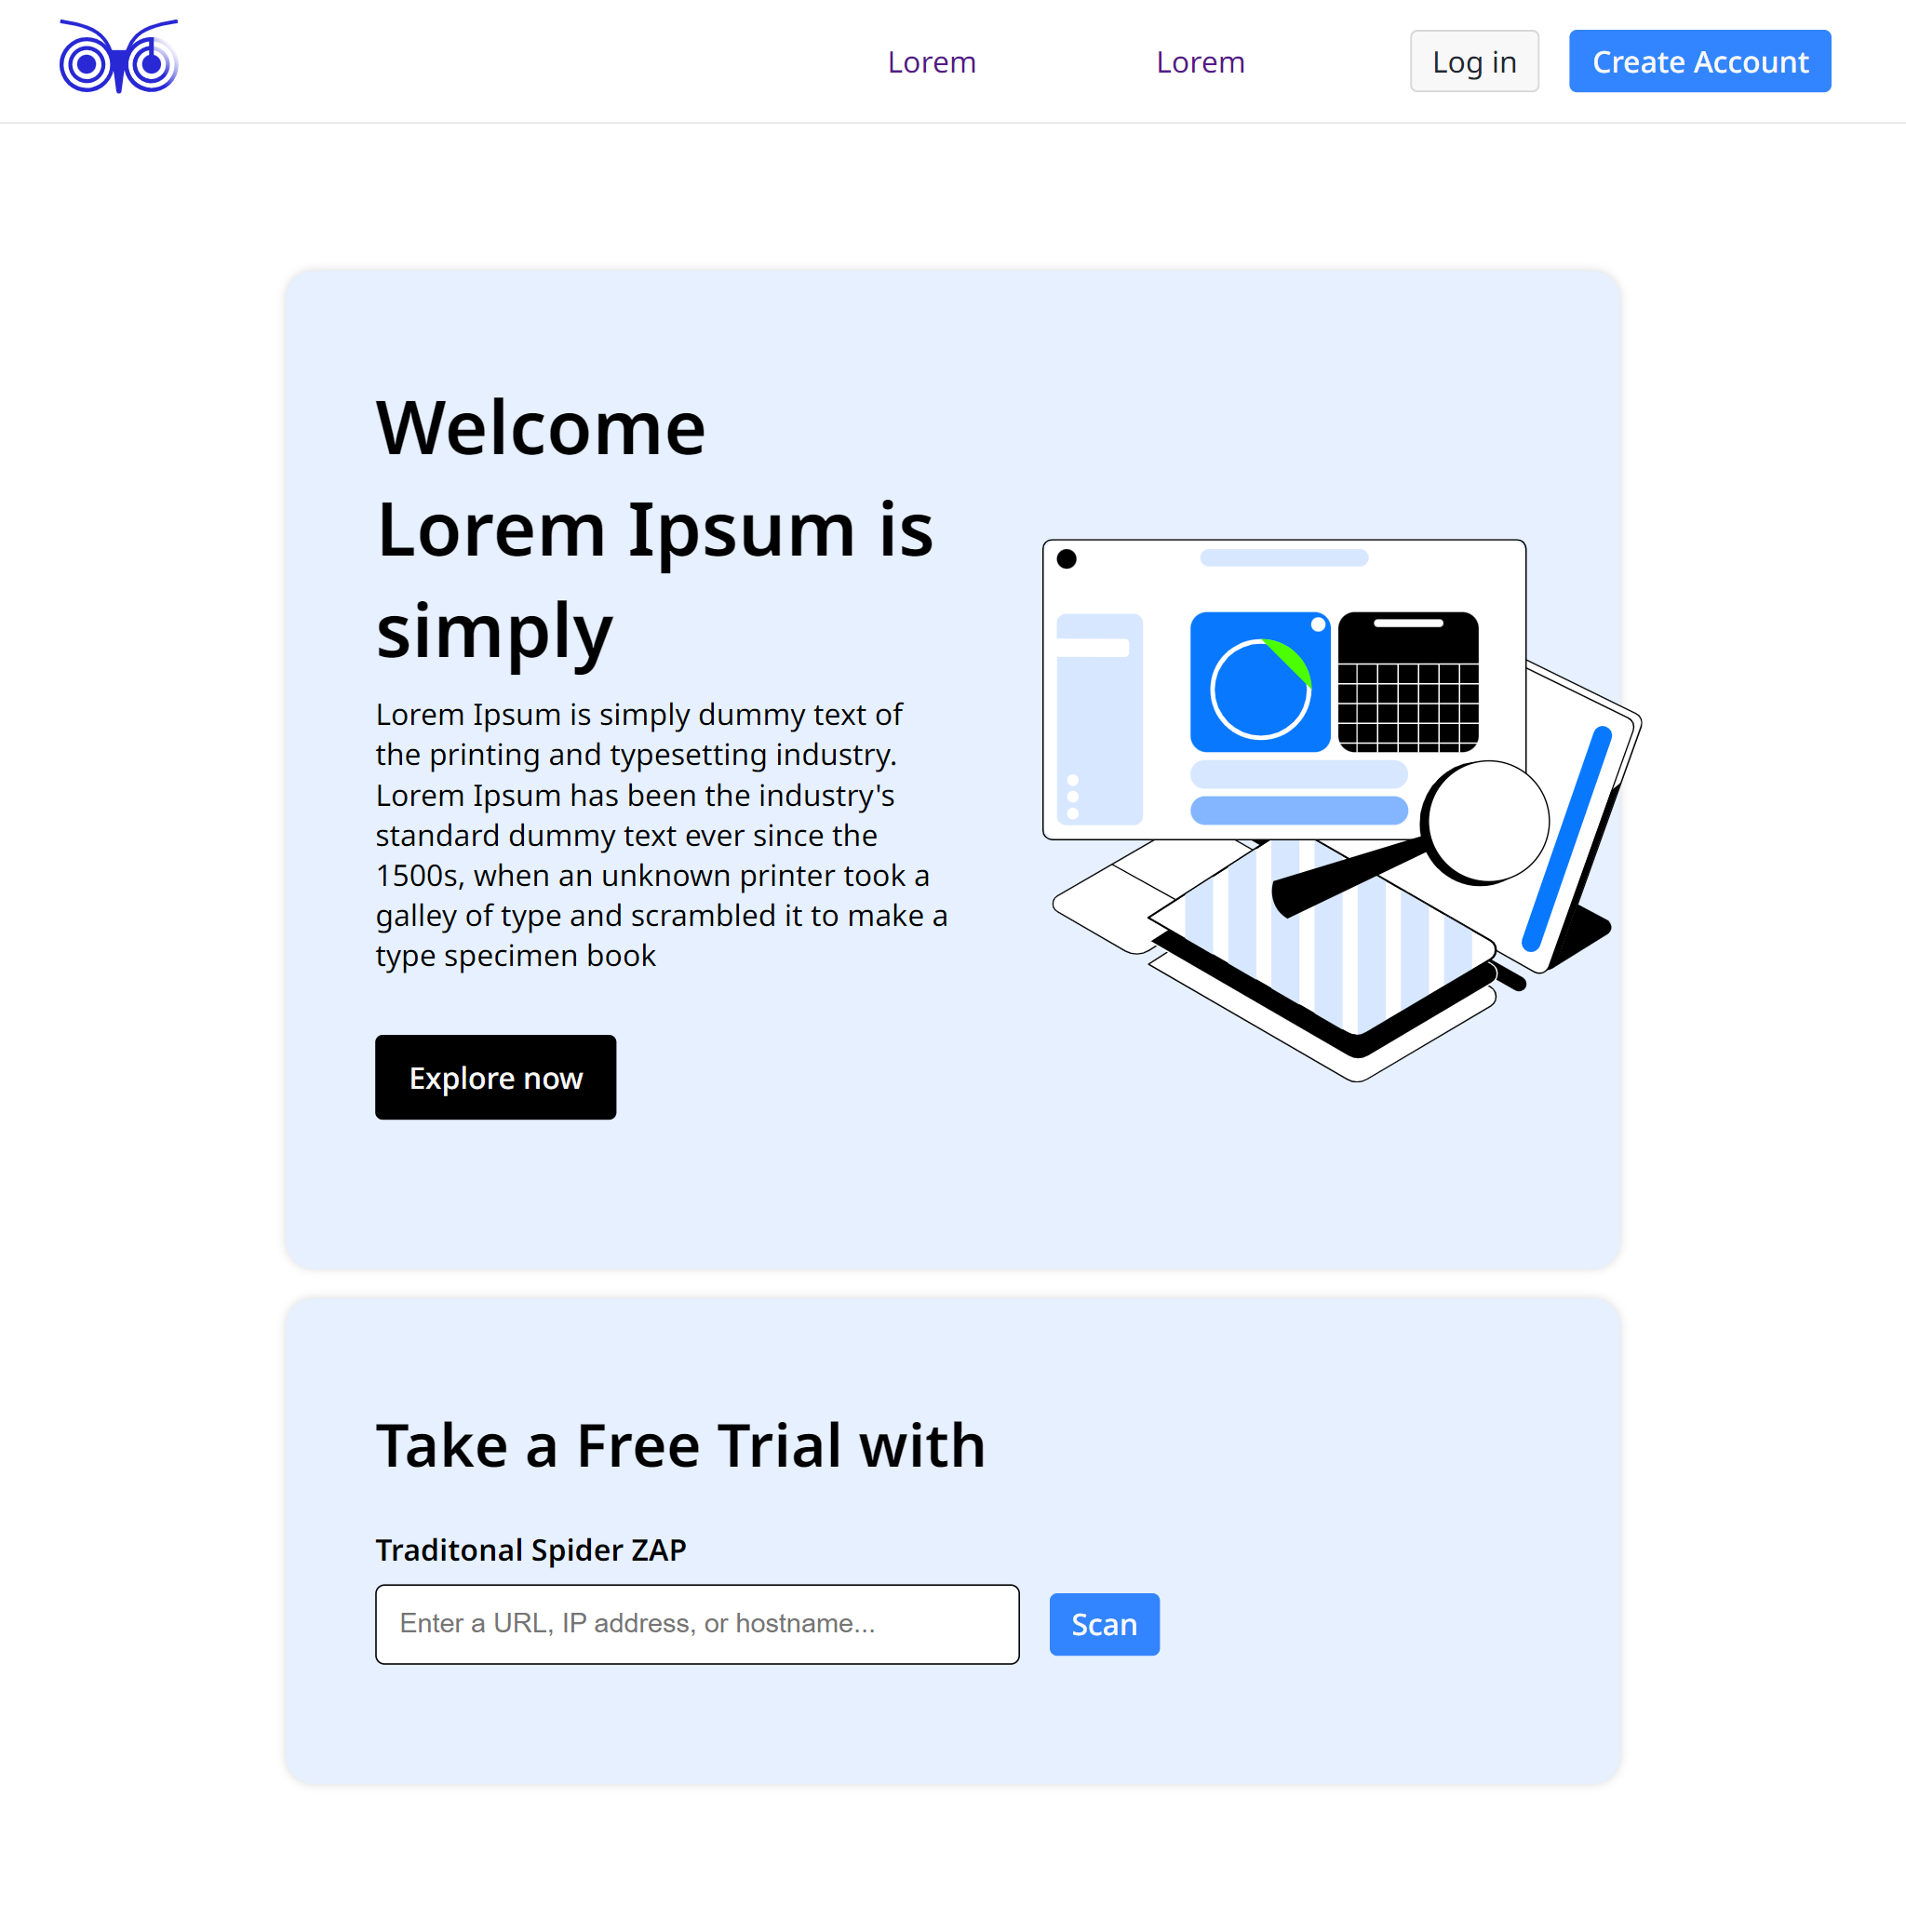
\includegraphics[width=\textwidth]{images/prototype/prototype_22112022/home.png}

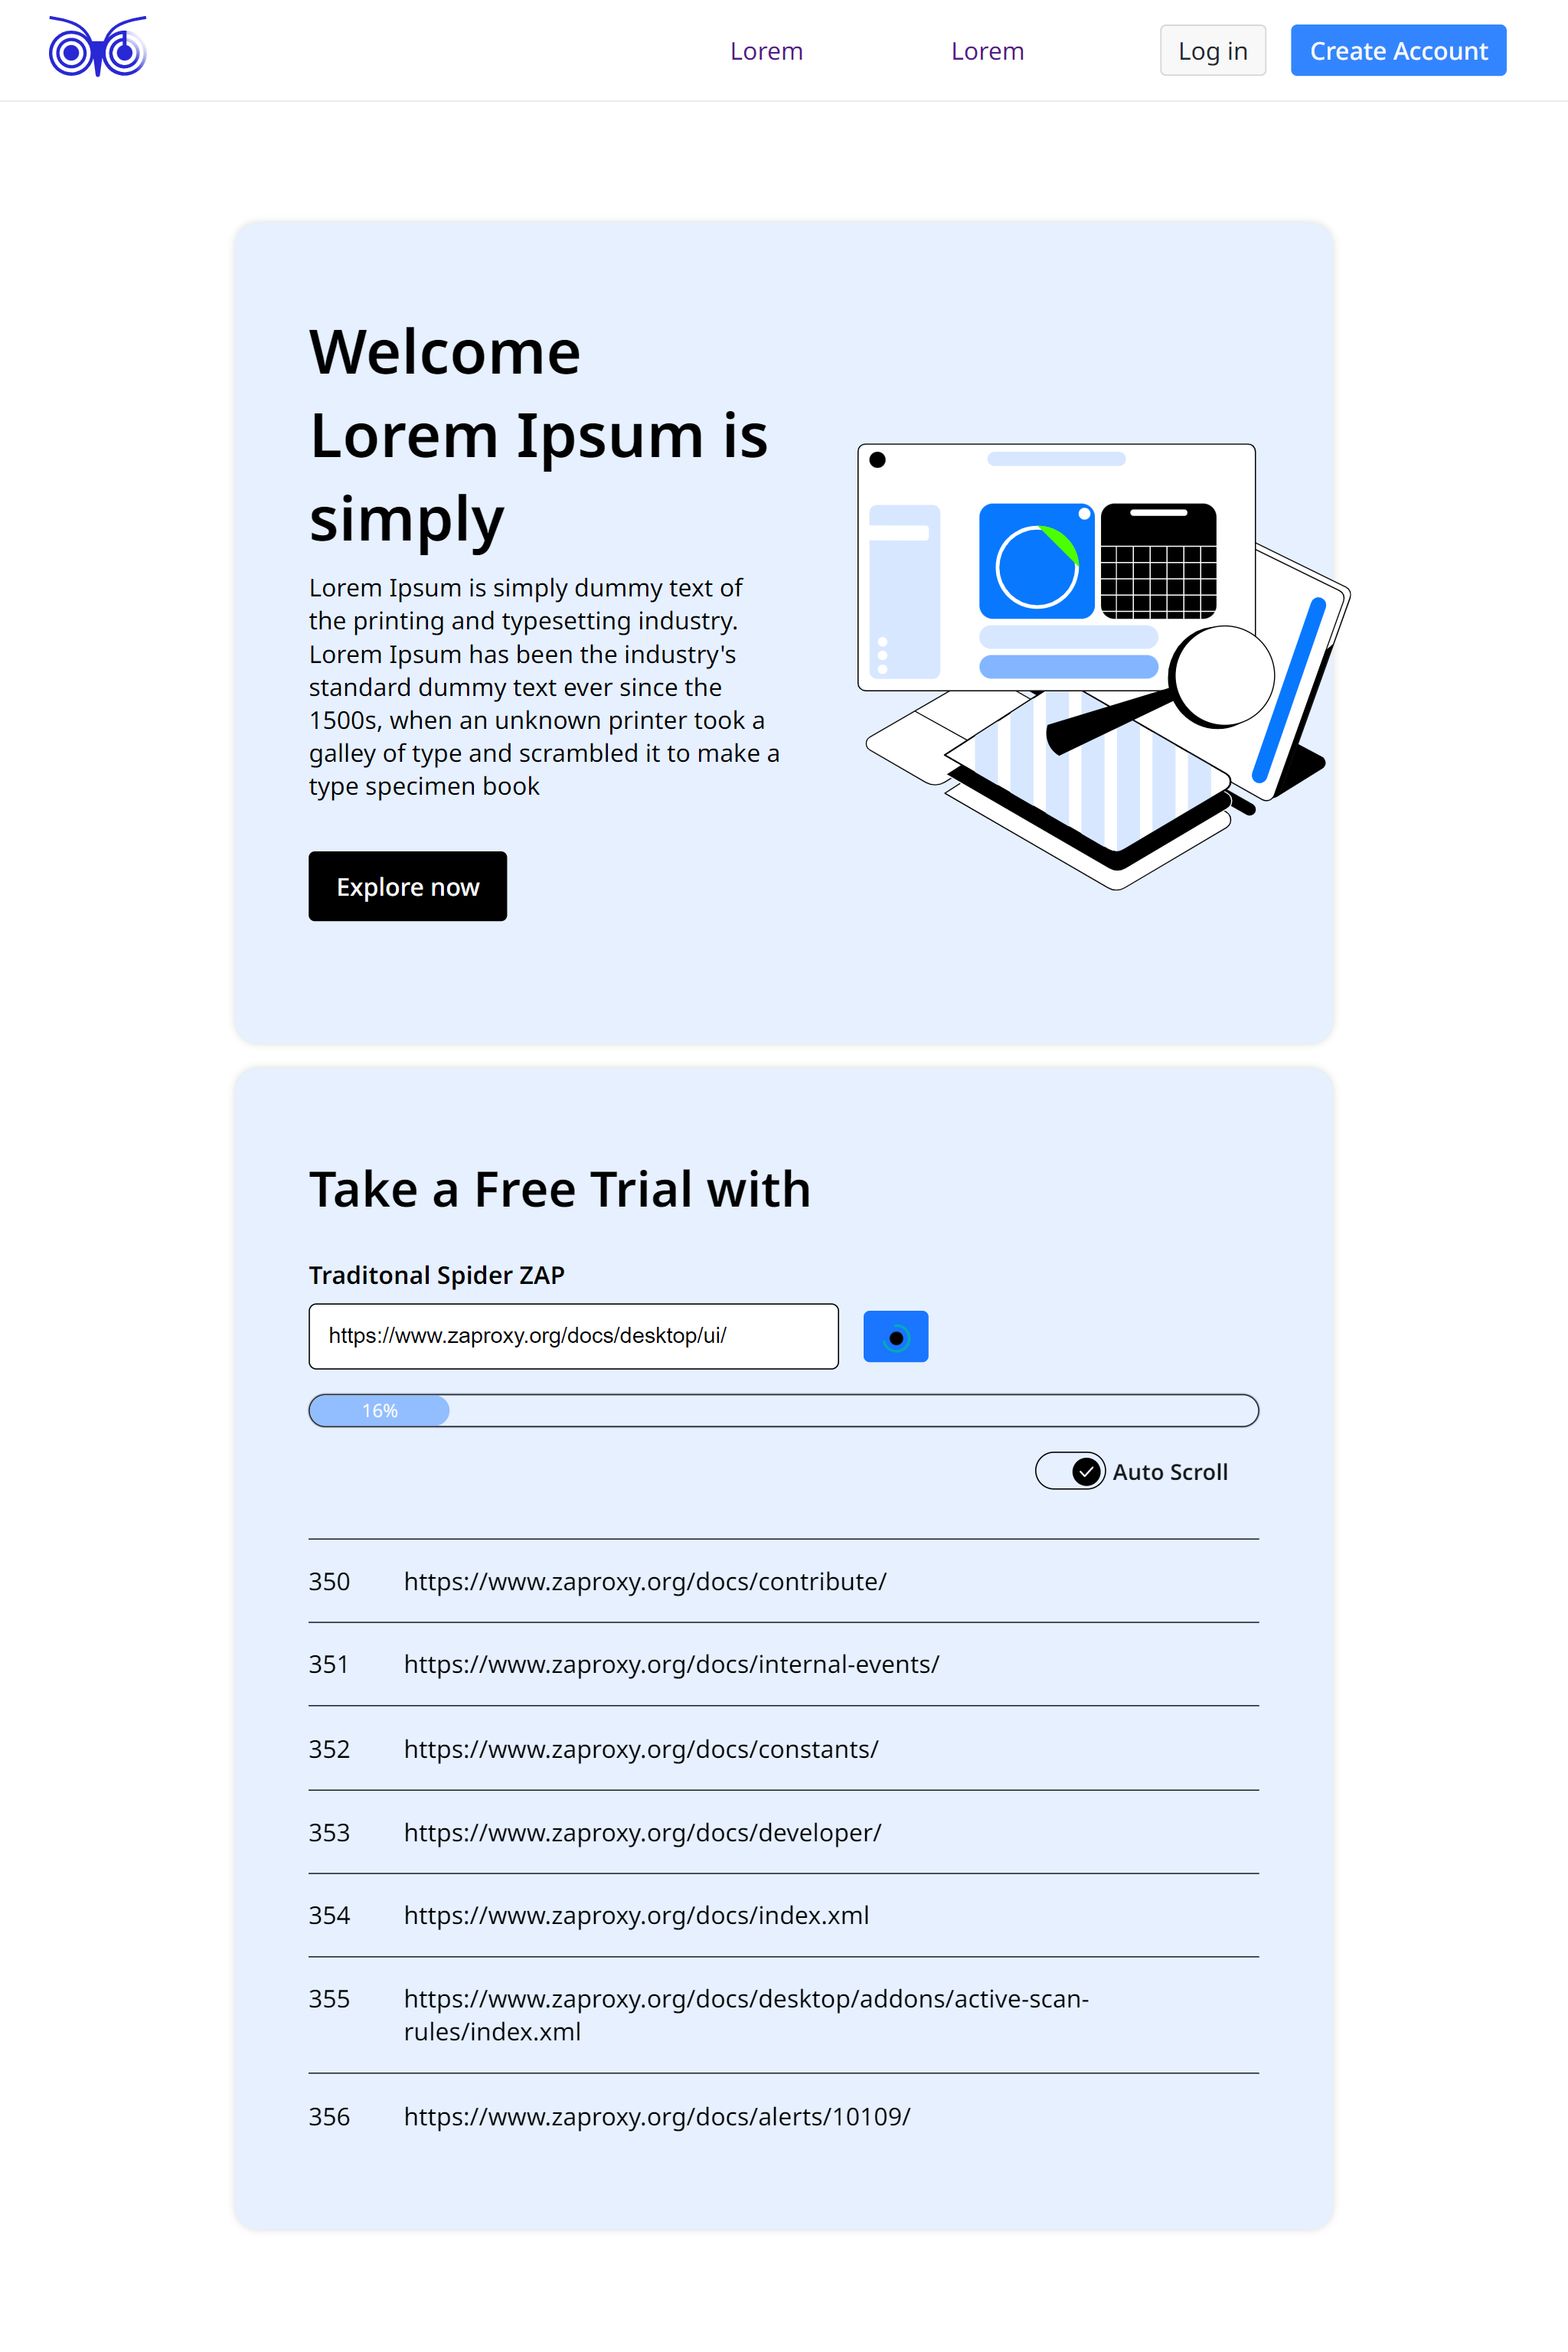
\includegraphics[width=\textwidth]{images/prototype/prototype_22112022/home_scanning.png}

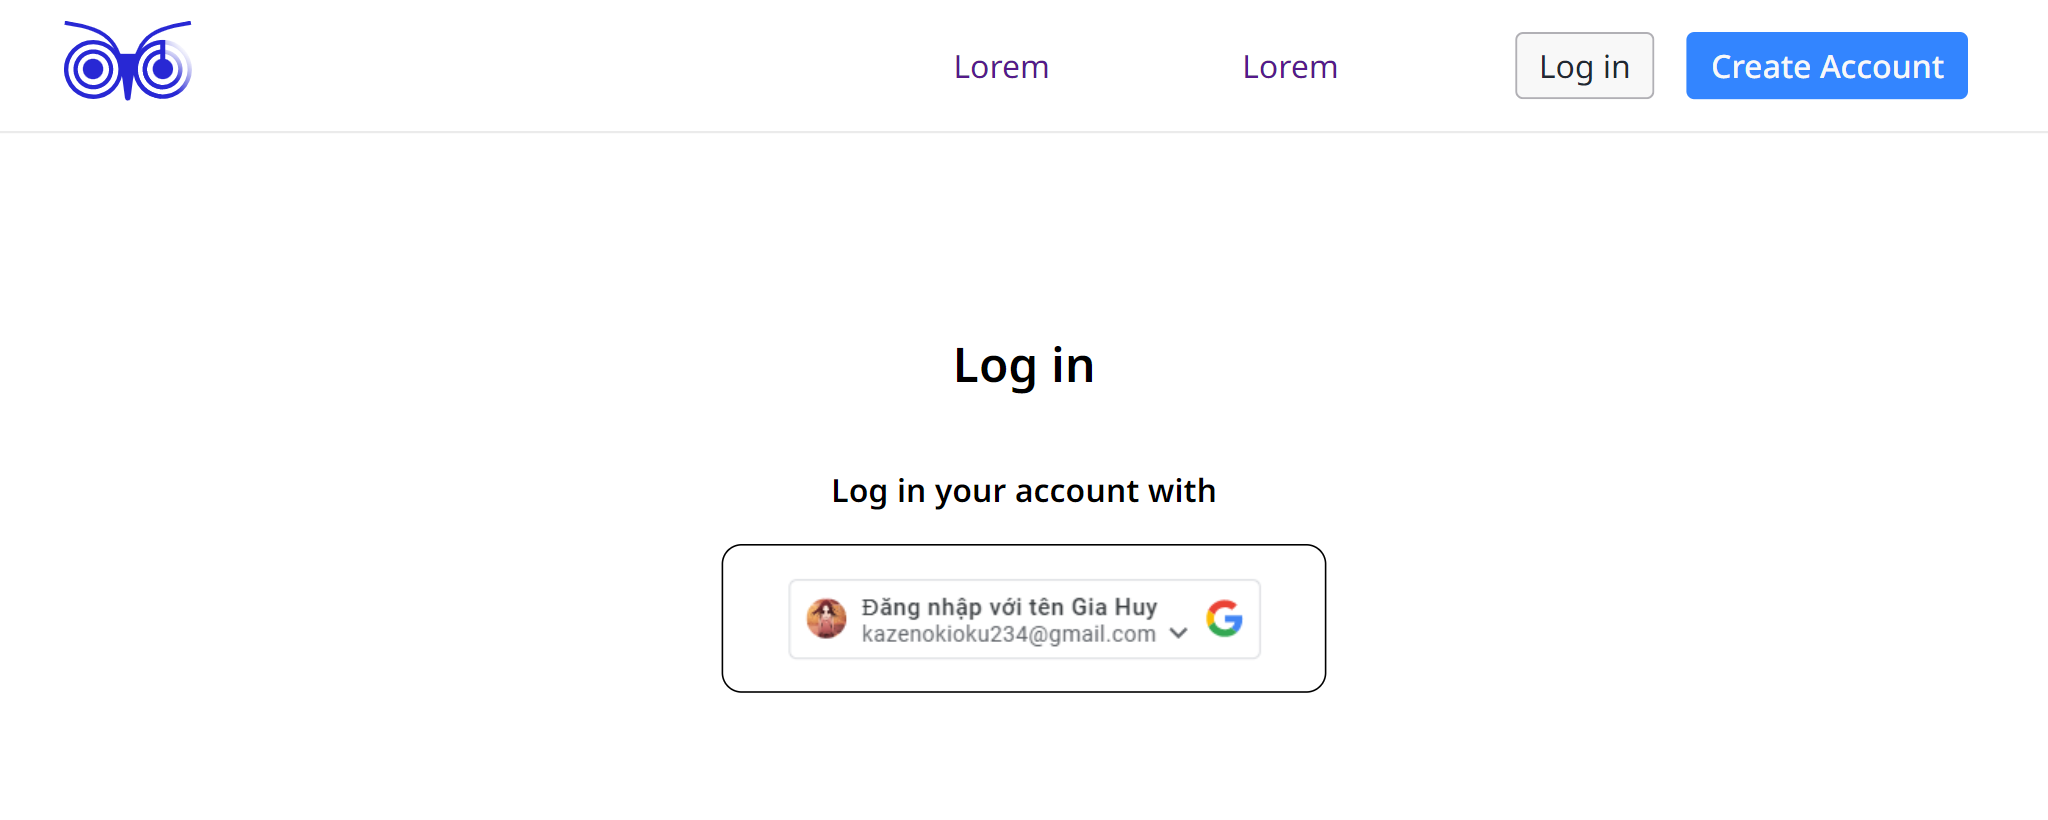
\includegraphics[width=\textwidth]{images/prototype/prototype_22112022/login.png}

\vspace{5cm}

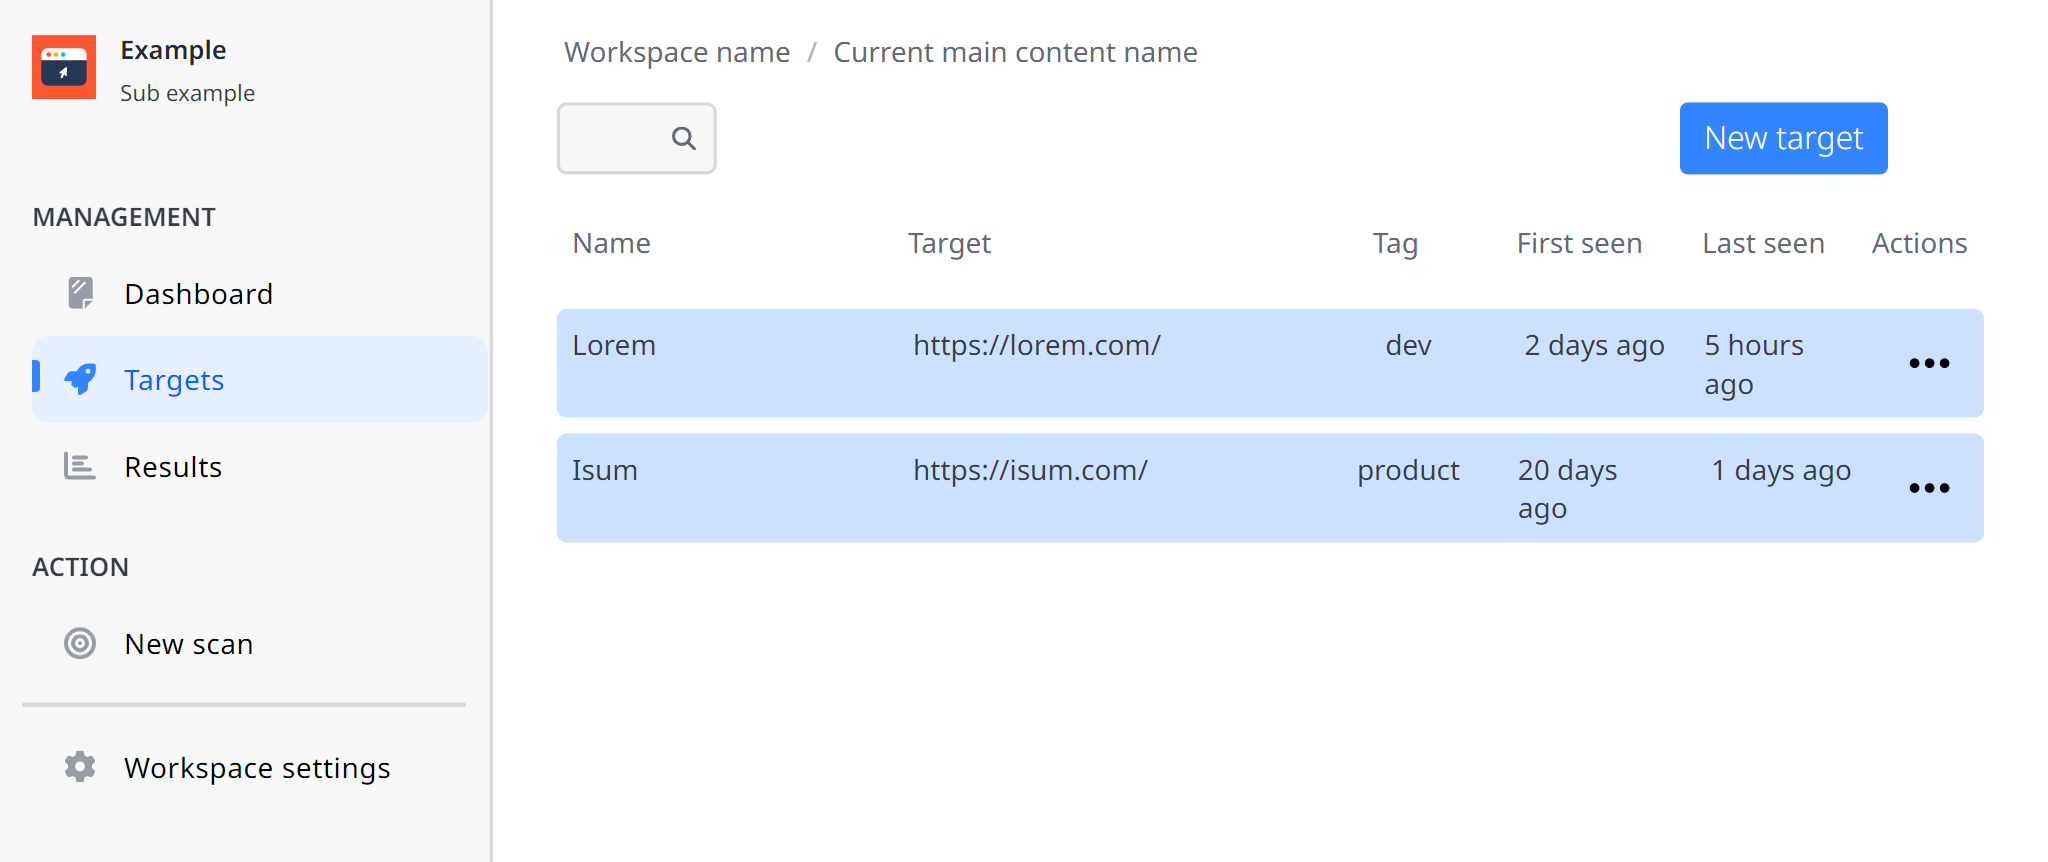
\includegraphics[width=\textwidth]{images/prototype/prototype_22112022/dashboard_target.png}

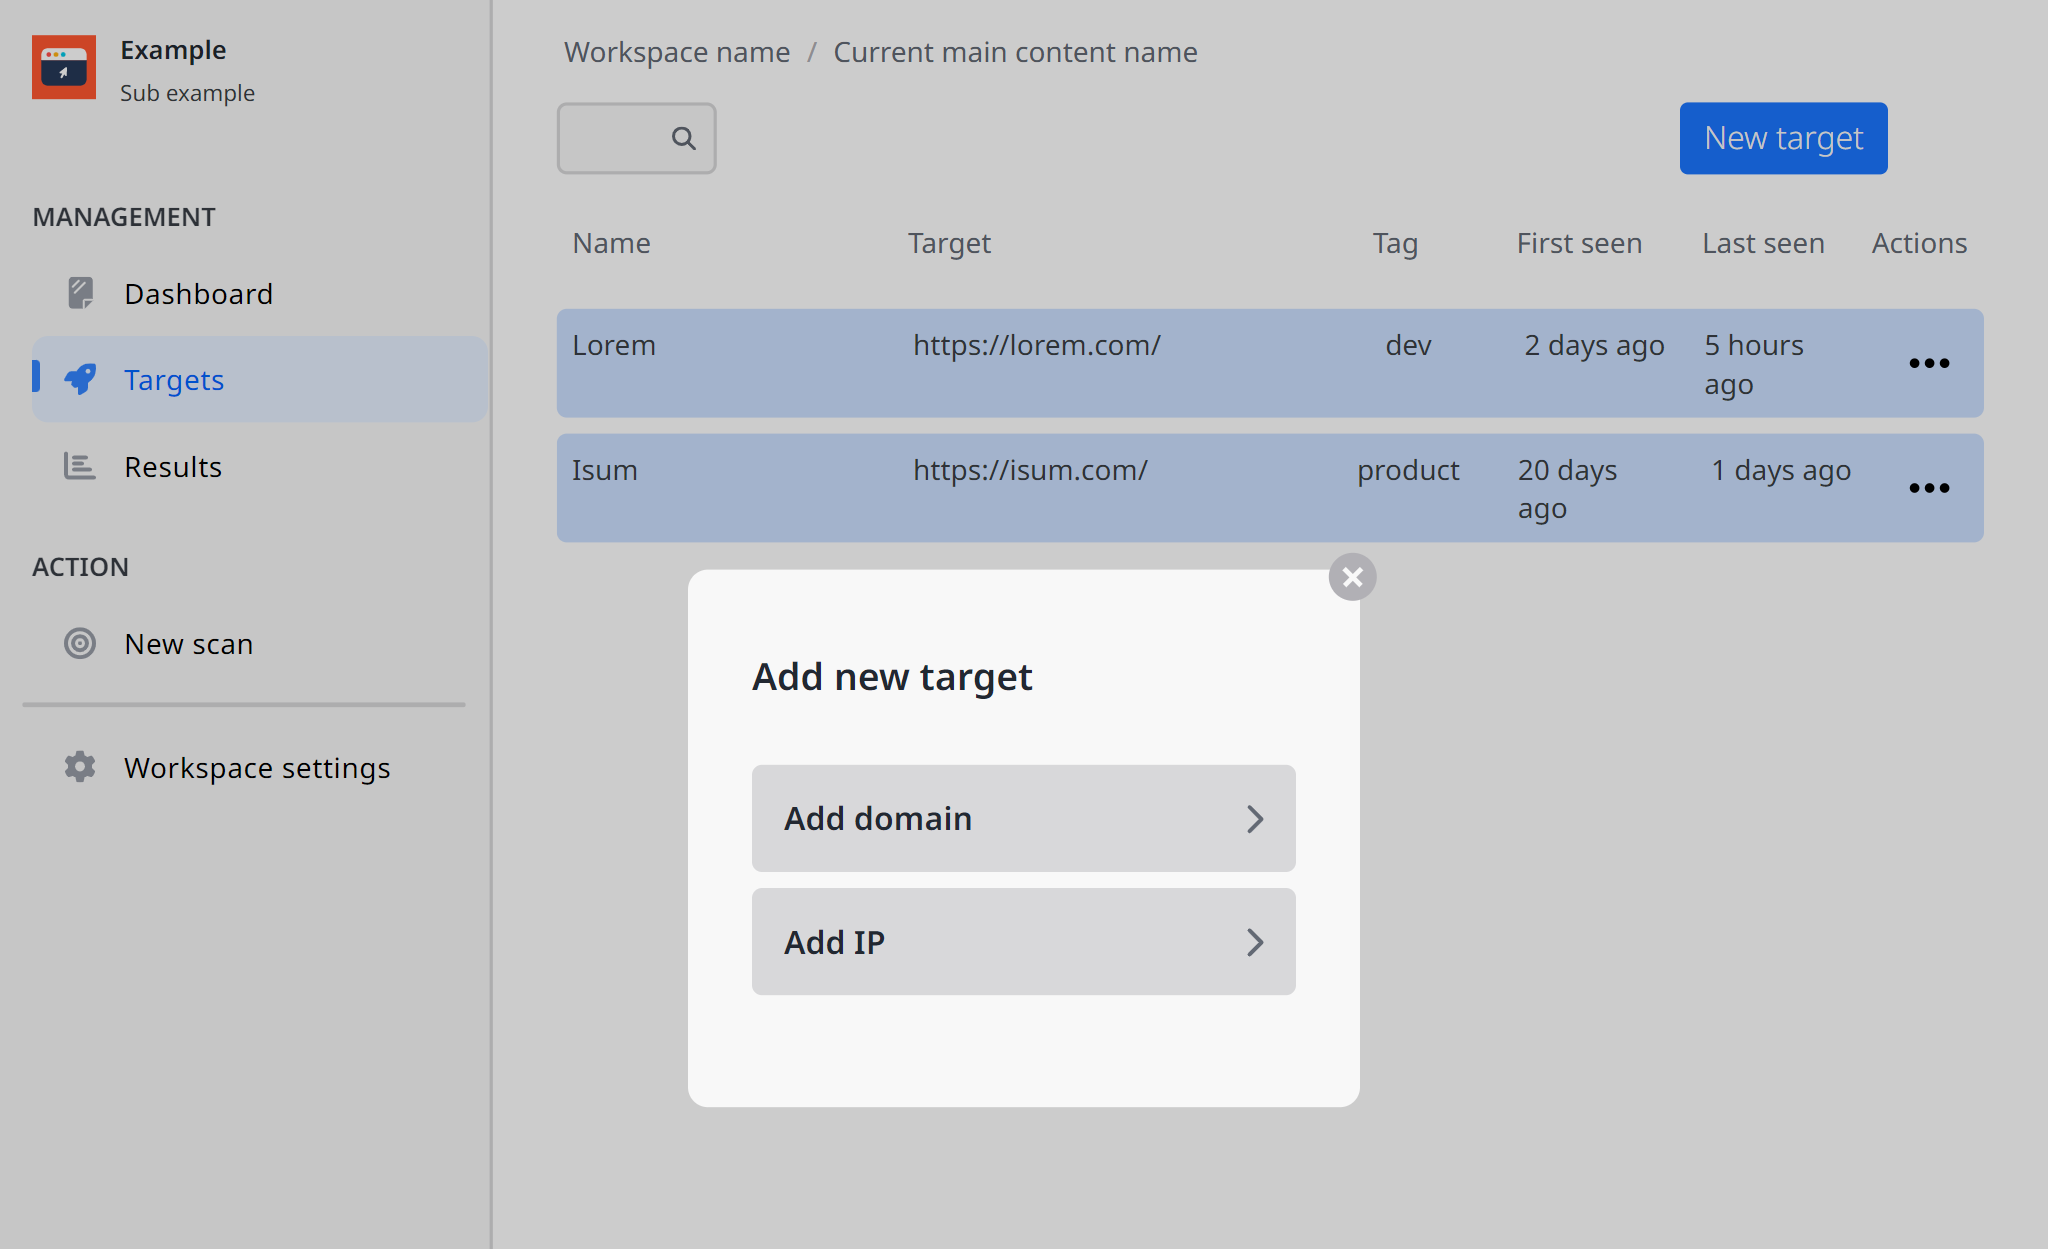
\includegraphics[width=\textwidth]{images/prototype/prototype_22112022/dashboard_target_add target.png}

\vspace{2cm}

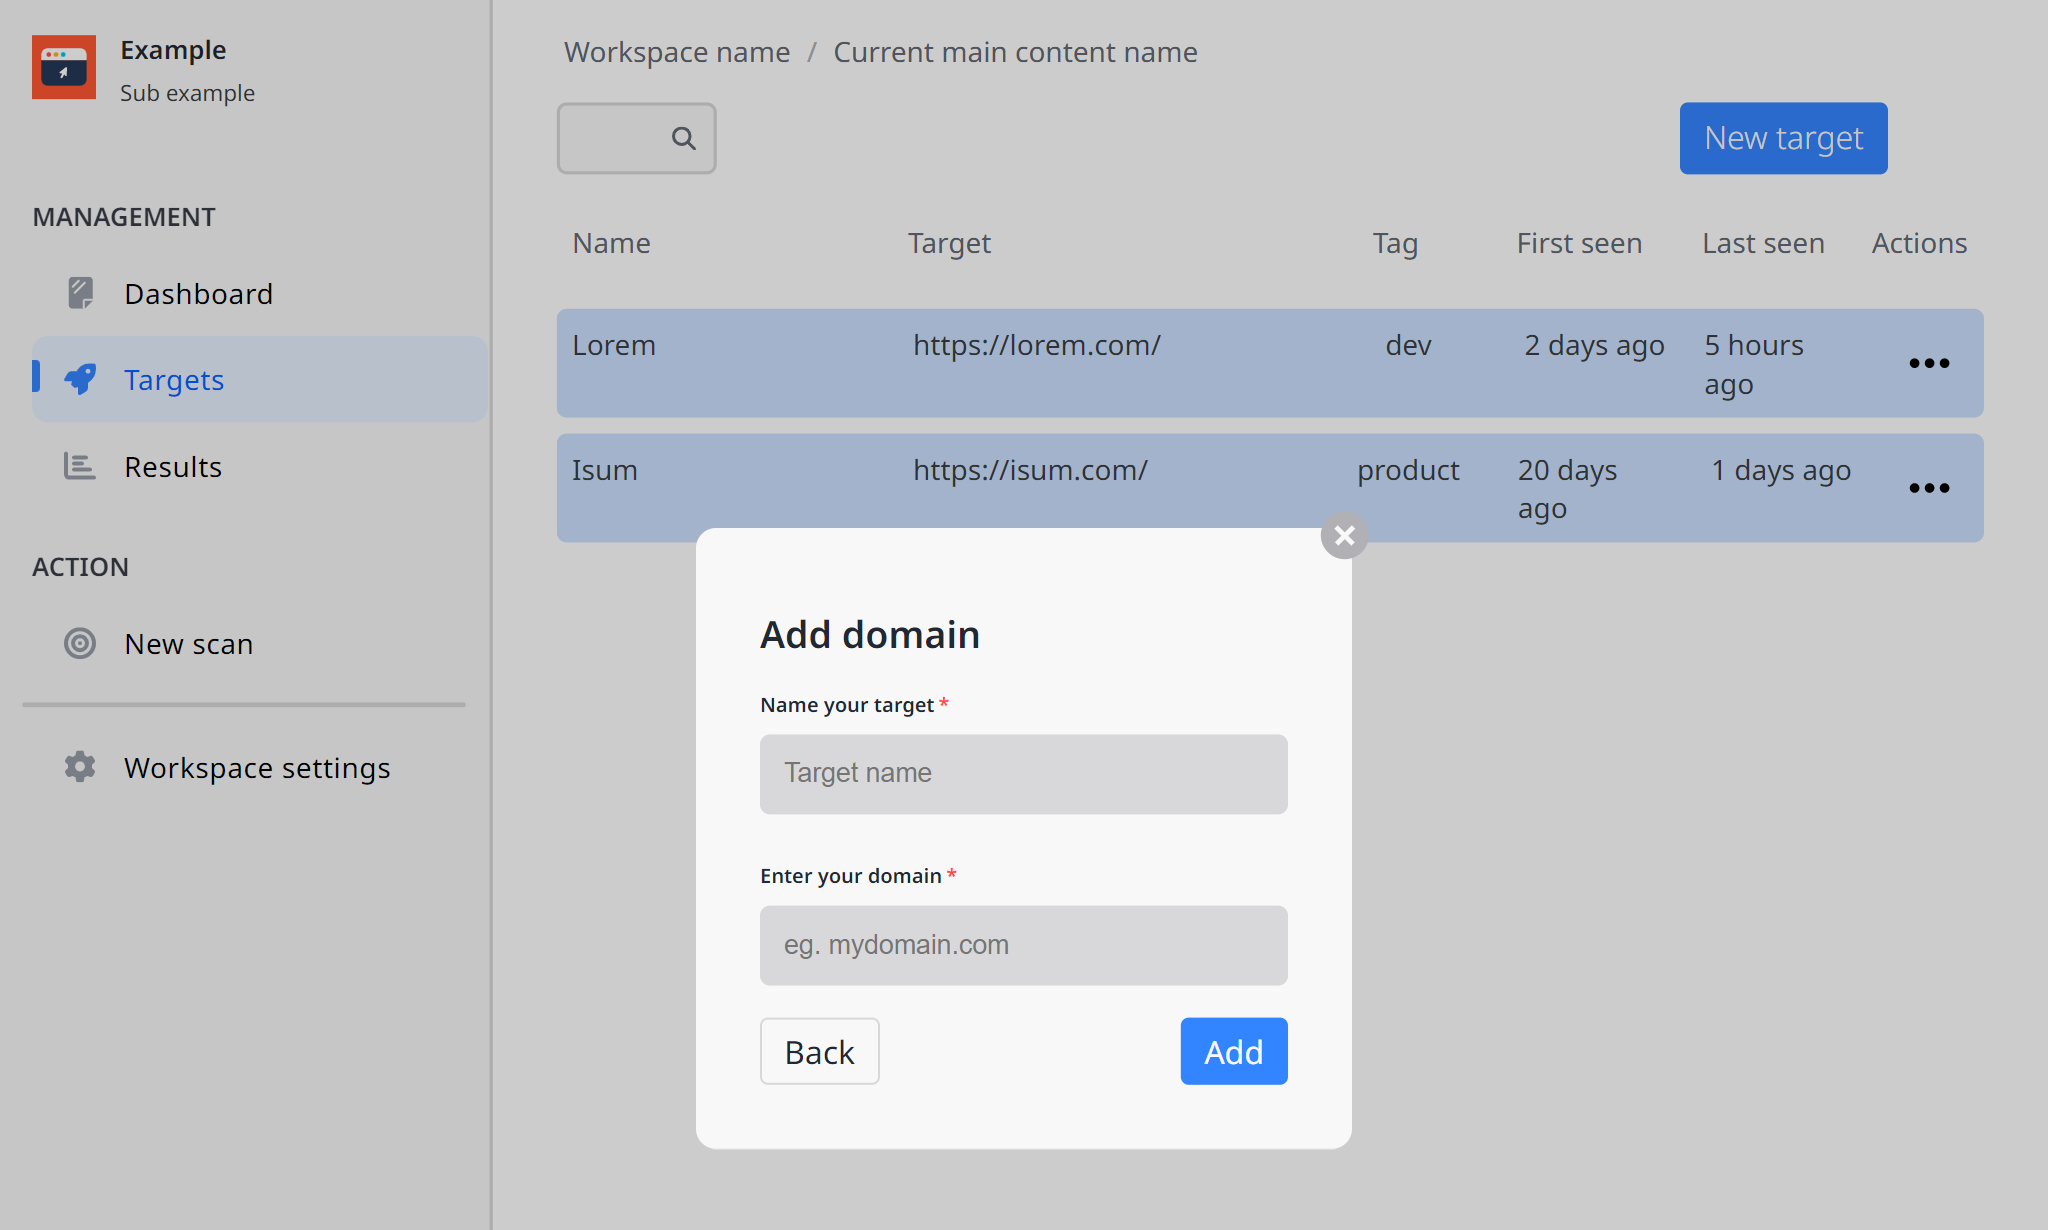
\includegraphics[width=\textwidth]{images/prototype/prototype_22112022/dashboard_target_add target_add domain.png}

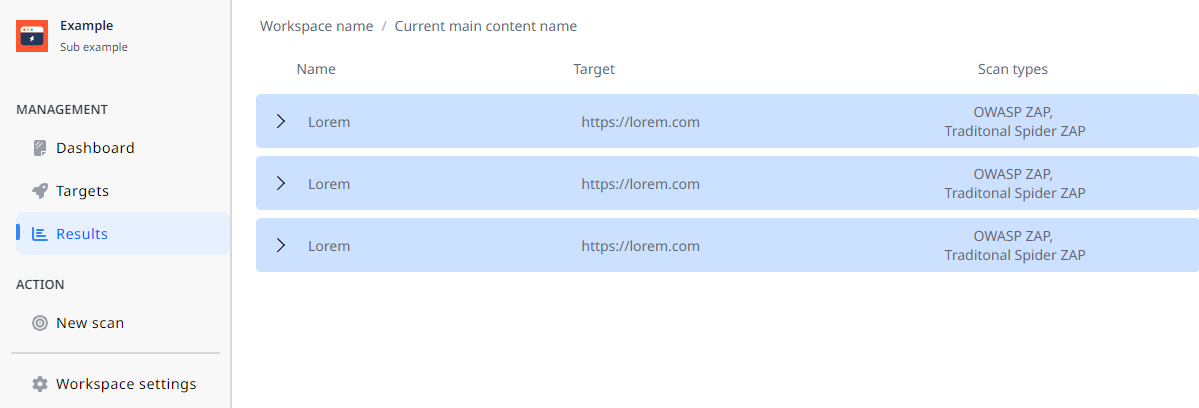
\includegraphics[width=\textwidth]{images/prototype/prototype_25102022/dashboard_result.png}

\vspace{1cm}

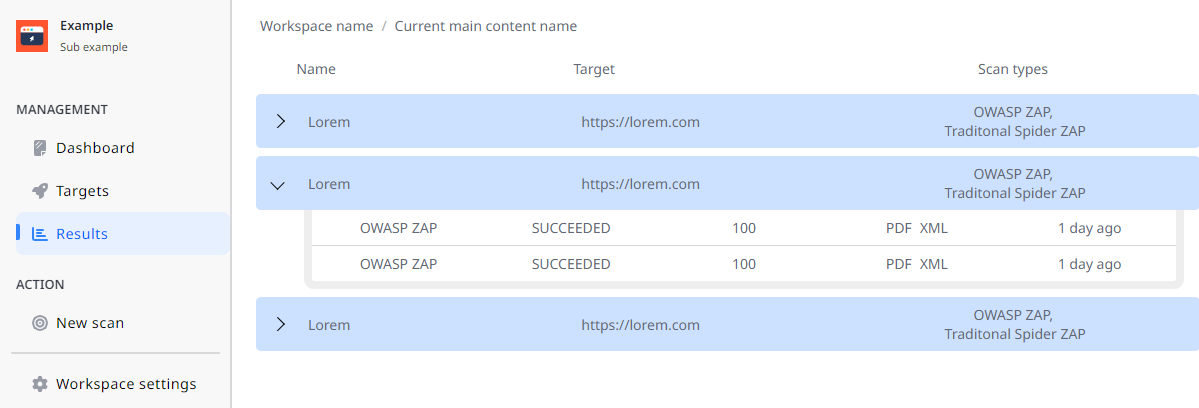
\includegraphics[width=\textwidth]{images/prototype/prototype_25102022/dashboard_result_opening-sub.png}

\vspace{1cm}

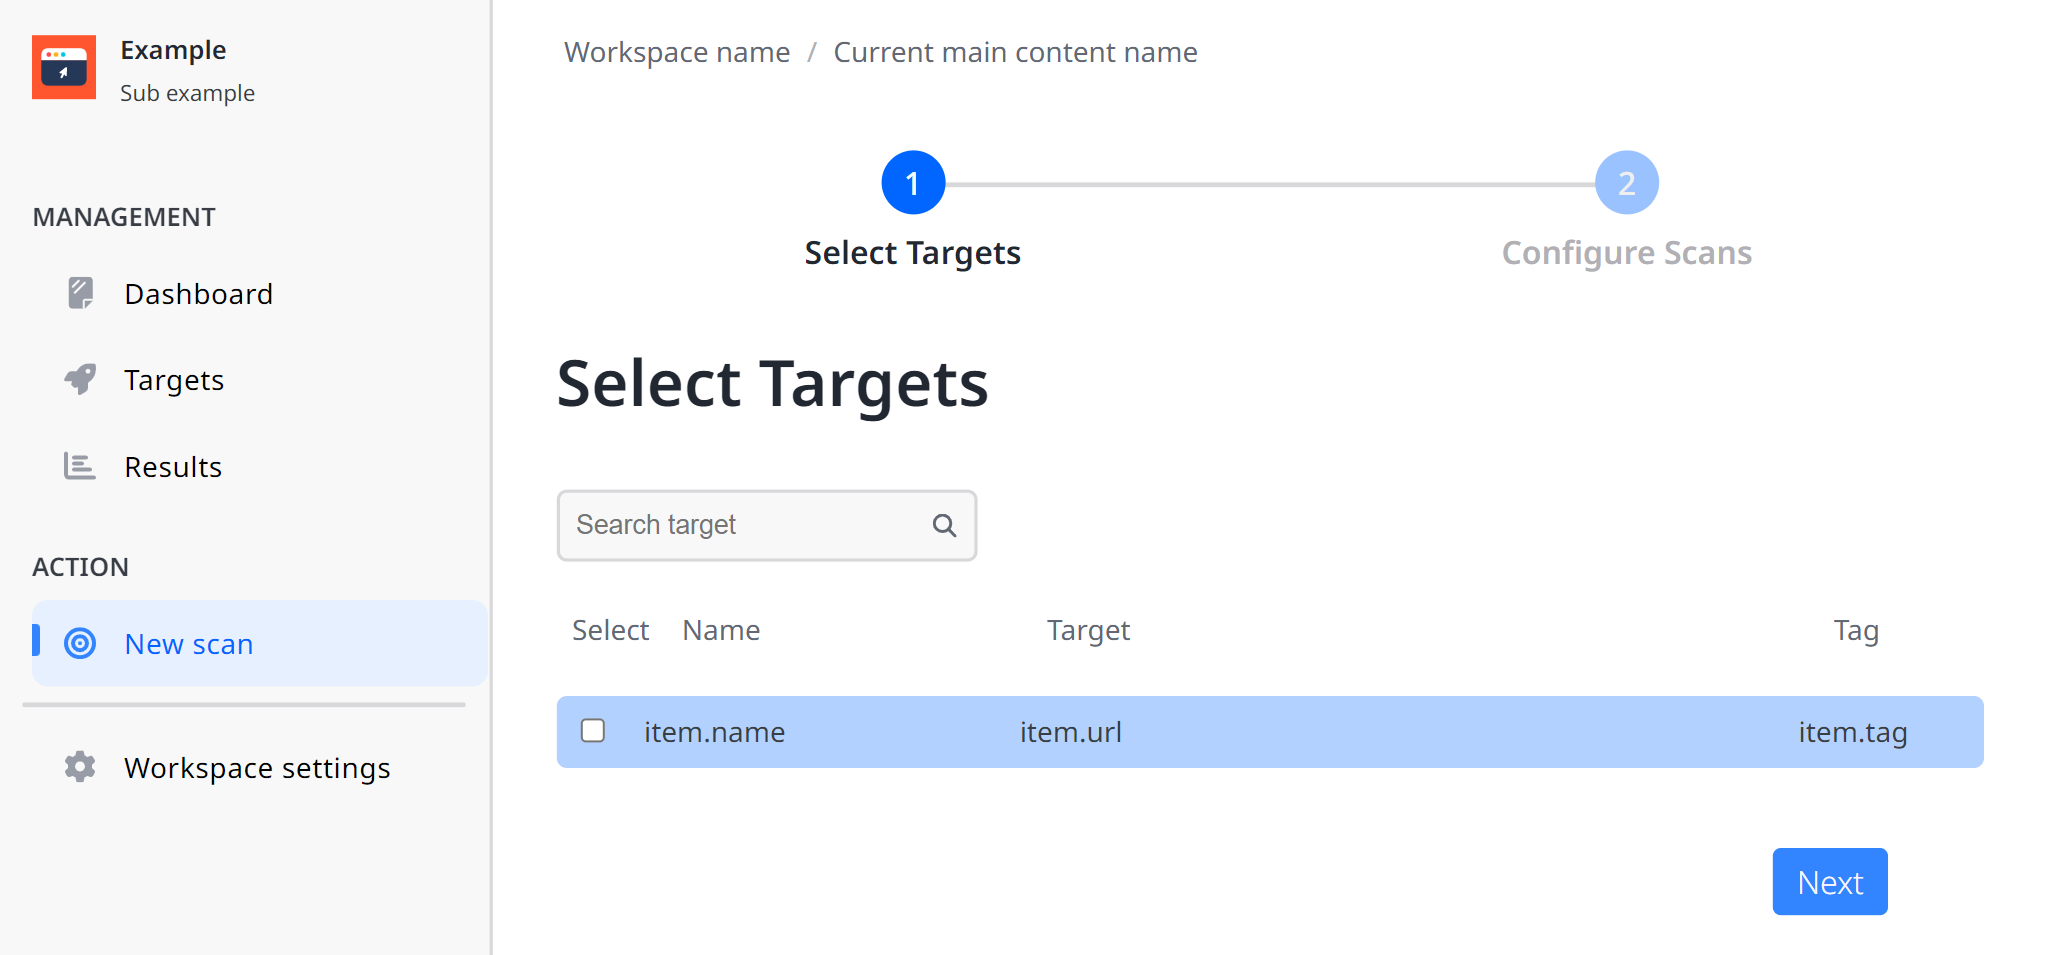
\includegraphics[width=\textwidth]{images/prototype/prototype_22112022/dashboad_new scan_select target.png}

\vspace{1cm}

\paragraph{Kiến trúc}
\tab Kiến trúc Scan Process
\vspace{3cm}

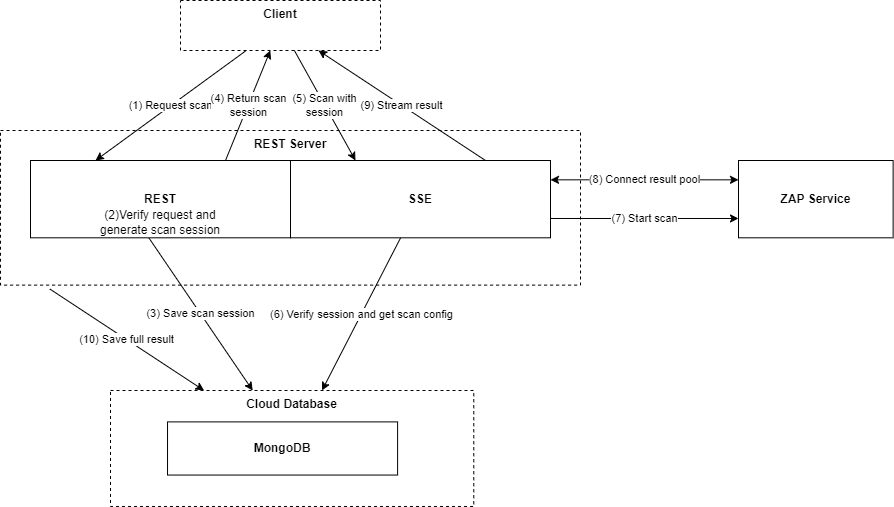
\includegraphics[width=\textwidth]{images/diagram/diagram_04112023/Scan Process.png}

\newpage
Kiến trúc triển khai
\vspace{3cm}

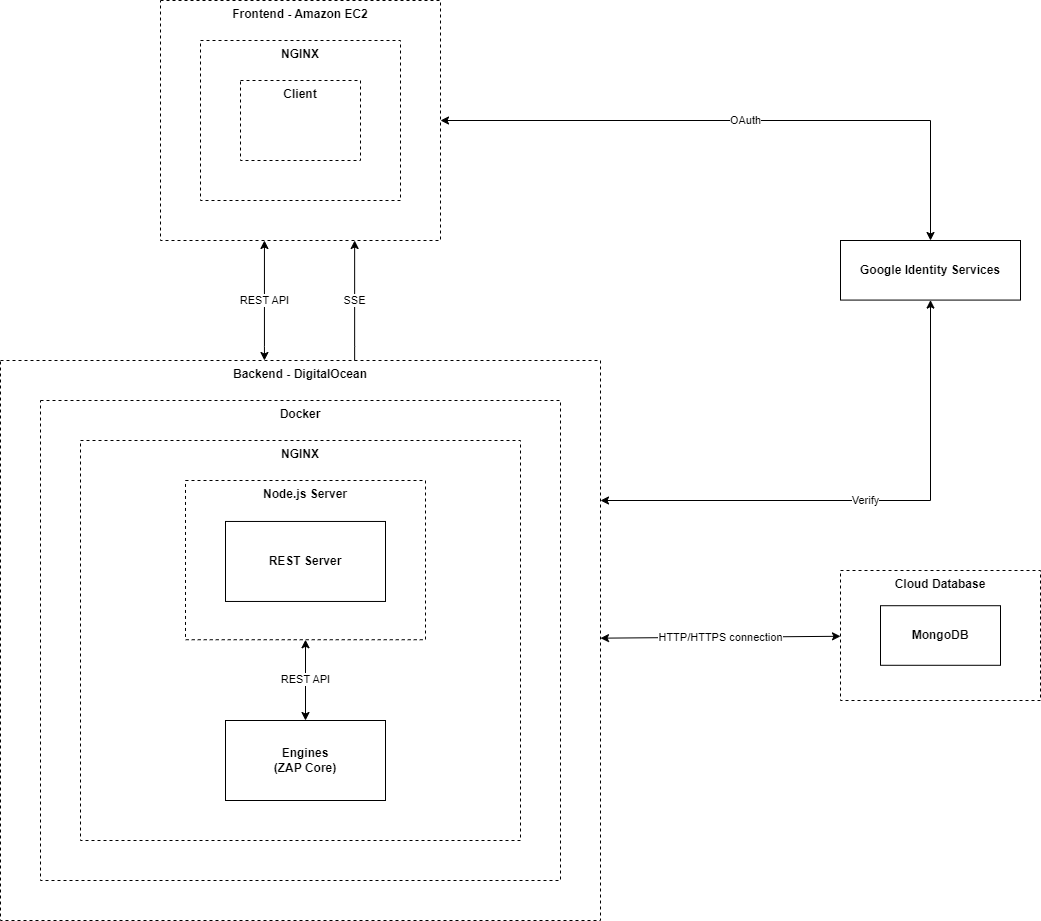
\includegraphics[width=\textwidth]{images/diagram/diagram_04112023/ZAPOP Architecture.png}

\paragraph{Mô hình dữ liệu}
\vspace{1cm}

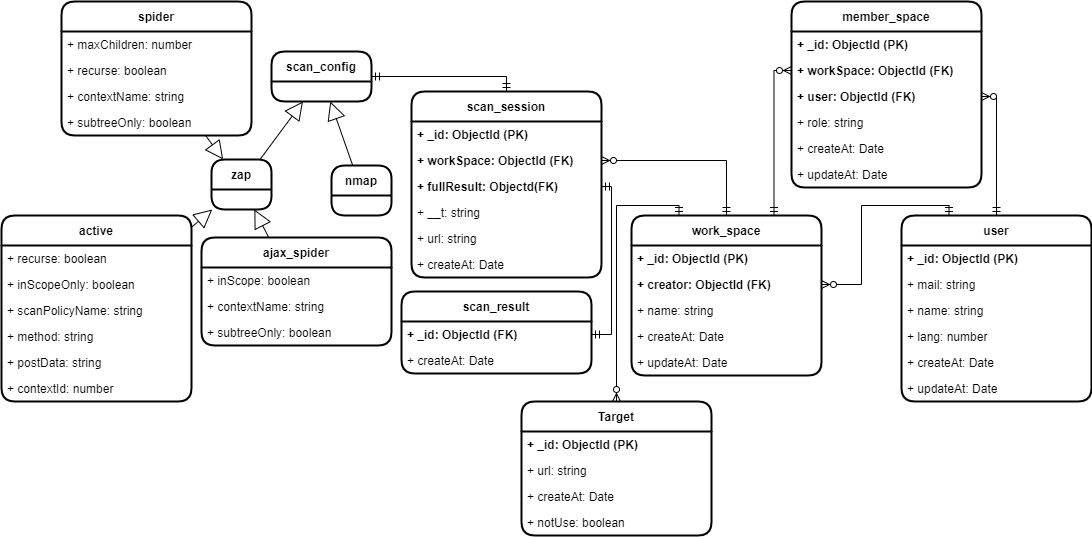
\includegraphics[width=\textwidth]{images/diagram/diagram_25102022/Database Diagram.png}

\vspace{0.1cm}

\paragraph{Các mục tiêu kiểm thử}
\begin{itemize}
    \item Load Testing: đo lường hiệu suất của ứng dụng để xác định tốc độ tương tác.
    \item Reliability Testing: đo lường mức độ xảy ra lỗi của ứng dụng để xác định mức độ lỗi tương tác.
\end{itemize}

\paragraph{So sánh, đánh giá hệ thống với các hệ thống tương tự}
\tab \textbf{Bảng so sánh các tính năng cơ bản của các hệ thống}
\begin{tabularx}{\textwidth}{|>{\hsize=.25\hsize\centering\let\newline
    \\\arraybackslash}X|>{\hsize=.15\hsize\centering\let\newline
    \\\arraybackslash}X|>{\hsize=.15\hsize\centering\let\newline
    \\\arraybackslash}X|>{\hsize=.15\hsize\centering\let\newline
    \\\arraybackslash}X|>{\hsize=.15\hsize\centering\let\newline
    \\\arraybackslash}X|>{\hsize=.15\hsize\centering\let\newline
    \\\arraybackslash}X|}
    \hline
    \textbf{Tính năng}
     & \textbf{\applicationname}
     & \textbf{Stack Hawk}
     & \textbf{Detectify}
     & \textbf{Hosted Scan}
     & \textbf{Idyllum Labs}
    \\
    \hline
    Quét với ZAP
     &
    \checkmark
     &
    \checkmark
     &
    \checkmark
     &
    \checkmark
     &
    \checkmark
    \\
    \hline
\end{tabularx}

\vspace{4cm}
\textbf{Bảng ưu điểm và khuyết điểm của các hệ thống}
\vspace{0.5cm}
\begin{tabularx}{\textwidth}{|>{\hsize=0.2\hsize\centering\let\newline
    \\\arraybackslash}X|>{\hsize=0.4\hsize\raggedright\let\newline
    \\\arraybackslash}X|>{\hsize=0.4\hsize\raggedright\let\newline
    \\\arraybackslash}X|}
    \hline
    \thead{Hệ thống}
     &
    \thead{Ưu điểm}
     &
    \thead{Khuyết điểm}
    \\
    \hline
    Stack Hawk
     &
    - Tự động quét trên mỗi PR hoặc trong CI/CD.
    \newlinecontenttable
    - Quản lý thông tin kết quả quét, giao diện tường minh, dễ sử dụng.
    \newlinecontenttable
    - Đề xuất liên kết chứa thông tin sửa lỗi tìm được.
    \newlinecontenttable
    - Tích hợp được với những công cụ quản lý khác có sử dụng CI/CD như: Jira Sotfware, Gitlab, Github Action, Azure Pinelines, Jenkins, Travis CI,\dots
    \newlinecontenttable
    - Tài liệu hướng dẫn đầy đủ, chi tiết.
     &
    - Cần cấu hình pineline (.yml, .yaml).
    \newlinecontenttable
    - Cần Docker image đã build xây dựng sẵn.
    \newlinecontenttable
    - Kích hoạt quét bằng command line ở máy local. Cấu hình kích hoạt quét gồm nhiều bước.
    \newlinecontenttable
    - Dùng thử một lần mỗi ngày.
    \\
    \hline
    Hosted Scan
     &
    - Hỗ trợ các loại quét khác như Nmap, OpenVas, SSL/TLS.
    \newlinecontenttable
    - Hẹn thời gian đặt lịch quét.
    \newlinecontenttable
    - Đề xuất liên kết chứa thông tin sửa lỗi tìm được.
    \newlinecontenttable
    - Thông tin scan đầy đủ. Giao diện đơn giản.
     &
    - Kết quả scan dường như là dữ liệu gốc, không được xử lý.
    \newlinecontenttable
    - Dùng thử 10 lần mỗi tháng.
    \\
    \hline
    Idyllum Labs
     &
    - Hỗ trợ các loại quét khác như Nmap, WhatWeb.
    \newlinecontenttable
    - Miễn phí hoàn toàn.
     &
    - Giao diện khó sử dụng.
    \newlinecontenttable
    - Chỉ chấp nhận tên miền gốc (.com,\dots)
    \newlinecontenttable
    - Không theo dõi được quá trình, tiến độ quét.
    \newlinecontenttable
    - Không lựa chọn hay cấu hình được phương thức quét. Tất cả các loại quét có hỗ trợ được quét chung trong một lần.
    \\
    \hline
\end{tabularx}

\paragraph{Đánh giá}
\tab - Các hệ thống tương tự đang có trên thị trường khá đa dạng.
Tuy nhiên, đa phần, mỗi hệ thống đều chỉ tập trung vào một chức năng nhất định trong các loại kiểm thử bảo mật.
Các hệ thống còn lại có chức năng bao quát như \applicationname có các tính năng mở rộng kèm theo thì yêu cầu nhiều bước cấu hình từ đầu gây ra việc khó sử dụng khi người dùng cần thực hiện công việc đơn giản nhanh chóng.
Tiếp đó là các hệ thống không trực quan trong quá trình quét hoặc là hiển thị kết quả quét chưa được xử lý hợp lý.
\newline

- Qua so sánh, đánh giá hệ thống của nhóm với các hệ thống tương tự. 
Các thành viên nhóm đã đưa ra thống nhất tổng quan về hệ thống \applicationname Thực hiện đúng các kế
hoạch đề ra theo các mục 2.2 Mục tiêu đề tài và 2.3 Phạm vi của đề tài.

\paragraph{Danh sách các công nghệ, công cụ sử dụng}
\begin{itemize}
    \item Jira Software: một công cụ trong bộ công cụ của ứng dụng quản lý Jira, sử dụng mô hình Kanban để thiết kế và triển khai đồ án.
    \item Confluence: một công cụ trong bộ công cụ của ứng dụng quản lý Jira, dùng để quản lý tài liệu.
    \item GitHub: dịch vụ lưu trữ và kiễm soát phiên bản mã nguồn sử dụng Git.
    \item GitHub Pages: dịch vụ được tạo bởi GitHub, cho phép xuất bản trang web hoặc ứng dụng website bằng cách lưu trữ mã nguồn trong GitHub.
    \item Node.js: môi trường thực thi mã JavaScript bên ngoài trình duyệt.
    \item MongoDB: cơ sở dữ liệu dạng NoSQL.
    \item MongoDB Atlas: cloud database của MongoDB.
    \item Mongoose: a Node.js-based Object Data Modeling (ODM) library for MongoDB.
    \item OWASP Zed Attack Proxy (ZAP): ứng dụng mã nguồn mở dùng để quét lỗ hổng bảo mật của ứng dụng website.
    \item Express.js: framework dành cho backend Node.js của ứng dụng website.
    \item Server-Send Events - SSEs: một loại thiết hệ thống được xây dựng trên kết nối HTTP. Duy trì kết nối giữa frontend và backend tuy nhiên chỉ có backend được phép gửi dữ liệu lên.
    \item Docker: nền tảng để cung cấp các bước triển khai ứng dụng dễ dàng hơn bằng cách sử dụng các containers.
    \item DigitalOcean: một nhà cung cấp dịch vụ cloud và Cơ sở hạ tầng Dịch vụ (Infrastructure as a Service - IaaS).
    \item Amazon - Elastic Compute Cloud - EC2: một dịch vụ AWS cung cấp môi trường cloud computing cho phép người dùng thuê và sử dụng các máy ảo (Virtual machine - VM) trên cloud.
    \item NGINX: một web server cũng có thể được dùng để revese proxy, load balancer, mail proxy.
    \item ReactJS: thư viện JavaScript dùng để xây dựng giao diện website cho người dùng.
    \item Redux: thư viện JavaScript dùng để quản lý và xử lý trạng thái ứng dụng.
    \item Google Identity Services API: dùng để thực hiện định danh bằng Google.
    \item Visual Studio Code: trình biên tập mã được phát triển bởi Microsoft.
\end{itemize}
\subsection*{2.5  Kết quả dự kiến của đề tài}
\begin{itemize}
    \item Hoàn thiện Hệ thống tự động tìm kiếm lỗi bỏ mật ứng dụng web dựa trên nền tảng ZAP hoàn chỉnh với các chức năng đã đặt ra.
    \item Hoàn thiện mã nguồn ứng dụng và triển khai trang website hệ thống.
    \item Tài liệu báo cáo chi tiết mà nhóm đã tìm hiểu trong suốt quá trình thực hiện đồ án. Kinh nghiệm tích lũy đạt được khi thực hiện một đồ án thực tế.
\end{itemize}
\subsection*{Kế hoạch thực hiện}
% \arraybackslash = \let\\\tabularnewline
% Use \newline to breakline within a cell
\begin{tabularx}{\textwidth}{|>{\hsize=.25\hsize\centering\let\newline
    \\\arraybackslash}X|>{\hsize=.5\hsize\raggedright\let\newline
    \\\arraybackslash}X|>{\hsize=.25\hsize\centering\let\newline
    \\\arraybackslash}X|}
    \hline
    % \multicolumn{1}{|c|}{\textbf{Thời gian}}
    % &
    % \multicolumn{1}{c|}{\textbf{Công việc}}
    % &
    % \multicolumn{1}{c|}{\textbf{Người thực hiện}}
    \thead{Thời gian} %Thời gian
     & \thead{Công việc} %Công việc
     & \thead{Người \\ thực hiện} % Người thực hiện
    \\
    \hline
    01/03/2023
    \newline
    -
    \newline
    15/03/2023
     &
    - Liên hệ giảng viên hướng dẫn xem xét, bàn luận để thống nhất nhận thực hiện đề tài.
    \newlinecontenttable
    - Tìm hiểu thêm về đề tài. Nghiên cứu quy trình thực hiện đồ án của giảng viên hướng dẫn.
     &
    Tất cả thành viên
    \\
    \hline
    15/03/2023
    \newline
    -
    \newline
    01/04/2023
     &
    - Giai đoạn khởi tạo dự án, khảo sát thị trường, tìm hiểu các sản phẩm tương tự.
    \newlinecontenttable
    - Khởi tạo và hoàn thành chương 1 báo cáo. Khởi tạo đề cương chi tiết, kế hoạch sơ bộ.
    \newlinecontenttable
    - Chuẩn bị bản mẫu Prototype và Proof of concept.
     &
    Tất cả thành viên
    \\
    \hline
    01/04/2023
    \newline
    -
    \newline
    15/04/2023
     &
    - Thiết kế luồng hoạt động dự kiến của sản phẩm.
    \newlinecontenttable
    - Tìm hiểu và lựa chọn về các công cụ, công nghệ, thư viện hỗ trợ xây dựng sản phẩm.
    \newlinecontenttable
    - Cập nhật chương 2, 3 báo cáo và đề cương chi tiết.
     &
    Tất cả thành viên
    \\
    \hline
    15/04/2023
    \newline
    -
    \newline
    01/05/2023
     &
    - Tổ chức mã nguồn, thiết kế giao diện trang chủ.
    \newlinecontenttable
    - Hoàn tất chương 2, cập nhật chương 3 và đề cương. Gửi giảng viên góp ý để chỉnh sửa tài liệu.
    \newlinecontenttable
    - Hoàn tất và nộp đề cương chi tiết cho khoa.
     &
    Tất cả thành viên
    \\
    \hline
    01/05/2023
    \newline
    -
    \newline
    15/05/2023
     &
    - Phát triển kiến trúc hệ thống. Triển khai CI/CD. Xây dựng các chức năng đã đề ra.
    \newlinecontenttable
    - Hoàn tất cơ bản giao diện hệ thống. Triển khai phiên bản thử nghiệm đầu tiên.
     &
    Tất cả thành viên
    \\
    \hline
    15/05/2023
    \newline
    -
    \newline
    15/06/2023
     &
    - Tiếp tục xử lí các vấn đề còn lại của sản phẩm, đánh giá chung và cải tiến với giảng viên.
    \newlinecontenttable
    - Hoàn tất chương 3 và cập nhật chương 4, 5.
     &
    Tất cả thành viên
    \\
    \hline
    15/06/2023
    \newline
    -
    \newline
    15/07/2023
     &
    - Thực hiện kiểm thử, triển khai phiên bản chính thức đầu tiên.
    \newlinecontenttable
    - Chuẩn bị và nộp đơn đăng ký bảo vệ đồ án.
     &
    Tất cả thành viên
    \\
    \hline
    15/07/2023
    \newline
    -
    \newline
    Thời gian còn lại
     &
    - Cập nhật, kiểm tra website và máy chủ lần cuối. Hoàn tất báo cáo đề tài.
    \newlinecontenttable
    - Thực hiện chỉnh sửa báo cáo đề tài lần cuối và chuẩn bị tài liệu cho buổi bảo vệ đề tài.
     &
    Tất cả thành viên
    \\
    \hline
    \caption{Dummy table}\label{dummy-1}\\
\end{tabularx}
% \newpage
\bibliographystyle{plain}
% \bibliography{bibliography.bib} %Comment this to avoid no /cite command error % \bibliography in this section is commented to revent "No /cite founds" build error

\setcounter{page}{1}
% APPLIED THESIS
\newpage
\pagestyle{plain}
\setcounter{page}{2}
\addcontentsline{toc}{chapter}{MỤC LỤC}
\tableofcontents
\newpage
\listoffigures
\newpage
\listoftables
\pagestyle{plain}
\newpage
\begin{center}
\textbf{\Large DANH MỤC KÝ TỰ VÀ CÁC TỪ VIẾT TẮT }
\vspace{1cm}
\end{center}

\begin{tabularx}{\textwidth}{>{\hsize=.10\hsize\centering\let\newline
    \\\arraybackslash}X>{\hsize=.80\hsize\raggedright\let\newline
    \\\arraybackslash}X}
    API
     &
     Application Programming Interface
     \\
     CI/CD
     &
     Continuous Integration and Continuous Deployment
     \\
     HTTP
    &
    Hypertext Transfer Protocol
    \\
     ID
      &
      Identification
     \\
     JWT
     &
     JSON Web Token
     \\
     OWASP
     &
     Open Web Application Security Project
      \\
    PDF
     &
     Portable Document Format
     \\
     URL
     &
     Uniform Resource Locator
     \\
     XML
     &
     Extensible Markup Language
     \\
    ZAP
     &
     OWASP Zed Attack Proxy
\end{tabularx}

\newpage
\addcontentsline{toc}{chapter}{TÓM TẮT KHÓA LUẬN}
\begin{center}
\textbf{\Large TÓM TẮT KHÓA LUẬN }
\vspace{1cm}
\end{center}

Luận văn là tài liệu chính của khóa luận, nội dung của luận văn sẽ đề cập tới các kiến thức, kỹ thuật liên quan trong quá trình thực hiện khóa luận. Luận văn của nhóm em bao gồm các phần như sau:

Chương 1 - Giới thiệu đề tài: Trình bày lý do xây dựng hệ thống tự động tìm kiếm lỗi bảo mật ứng dụng web dựa trên nền tảng ZAP. Trình bày các tính năng cơ bản của 3 hệ thống tự động tìm kiếm lỗi bảo mật ứng dụng web tương tự hiện có. Đánh giá ưu điểm và các điểm chưa hoàn thiện của 3 hệ thống trên. Trình bày mục tiêu và phạm vi phát triển của đề tài.

Chương 2 - Lý thuyết nền tảng: Trình bày tóm tắt lý thuyết và thông tin về các lỗi bảo mật web phổ biến, kiến trúc phân tầng (N-Tier) và kiến trúc nguồn sự kiện (Event Sourcing).
Cùng với đó, trình bày giới thiệu tổng quan và các chức năng của công cụ OWASP Zed Attack Proxy, và phân tích ưu nhược điểm của công cụ.

Chương 3 - Thiết kế giải pháp: Nếu ra các giải pháp chức năng cho ứng dụng hệ thống, thiết kế kiến trúc hệ thống, thiết kế giao diện hệ thống và các sơ đồ thiết kế liên quan.

Chương 4 - Cài đặt giải pháp: Đề cập các công cụ dùng để cài đặt từng giải pháp hoặc thành phần đã nói ở trong chương 3, đề cập cách hoạt động, cách cài đặt chi tiết của các chức năng. Bên cạnh đó, chương 4 còn đề cập đến một số khó khăn đáng kể trong quá trình cài đặt và giải pháp cho chúng.

Chương 5 - Tổng kết và đánh giá: Phần này liệt kê các kiến thức mà chúng em đạt được trong quá trình thực hiện luận văn, sản phẩm thu được từ quá trình thực hiện luận văn, những chức năng đã thực hiện. Cùng với đó, chương còn so sánh ứng dụng của luận văn với một số ứng dụng hiện có trên thị trường, phương hướng phát triển trong tương lai.

Chương 6 - Phụ lục: Trình bày giới thiệu, khái niệm, sơ lược các chức năng và cách sử dụng của thư viện RTK Query và RxJS.
Nội dung trình bày các chức năng và cách sử dụng của các thư viện chủ yếu nằm trong phạm vi khóa luận.
Dùng hỗ trợ phần trình bày ở Chương 4 được ngắn gọn và rõ ràng.
Đồng thời, trình bày giao diện và chức năng của ứng dụng sản phẩm.


\chapter{TỔNG QUAN}
\pagenumbering{arabic}

\section{Giới thiệu đề tài}

\tab Khi phát triển phần mềm hay ứng dụng, bước cần thiết nhất và không thể thiếu trước khi triển khai sản phẩm vào thực tế là kiểm thử.
Có rất nhiều vấn đề ta cần quan tâm khi tiến hành kiểm thử một ứng dụng, vấn đề bảo mật là một trong số đó.
Bảo mật của một ứng dụng là một vấn đề quan trọng thấy rõ mà nhiều ứng dụng bỏ qua hoặc chưa xử lý, phát hiện được triệt để các lỗi này.
Vì vậy, với tâm lý này làm cho sự xuất hiện của các người dùng tiêu cực và nhà phát triển tiêu cực ngày càng nhiều và phát triển nhanh chóng, hậu quả gây ra là khôn lường.
Do đó, nhóm sinh viên muốn tạo ra một hệ thống kiểm thử bảo mật trực tuyến, giúp cho việc kiểm thử diễn ra dễ dàng, nhanh gọn, trực quan hơn.
Tên là Owlens - Hệ thống tự động tìm kiếm lỗi bảo mật ứng dụng web dựa trên nền tảng OWASP ZAP (Automated web application security scanner based on ZAP).

\newpage
\section{Khảo sát thị trường}
\subsection{“Detectify” do Detectify phát triển}

\tab Được thành lập vào năm 2013 tại Thụy Điển.
Nền tảng cung cấp hơn 1700 mô-đun cũng như là phương thức, kịch bản tấn công được phát triển bởi hơn 400 chuyên gia tìm kiếm lỗ hổng ở một cộng đồng riêng của nền tảng.
Các lỗ hổng tìm thấy được lưu trữ và cho phép người dùng quản lý, xem thông tin chi tiết, tương tác với các hệ thống quản lý lỗi, quản lý phần mềm khác.
Cung cấp giải phát tự động quét theo lịch hẹn trước hoặc kết hợp với CI/CD.

\begin{figure}[H]
    \centering
    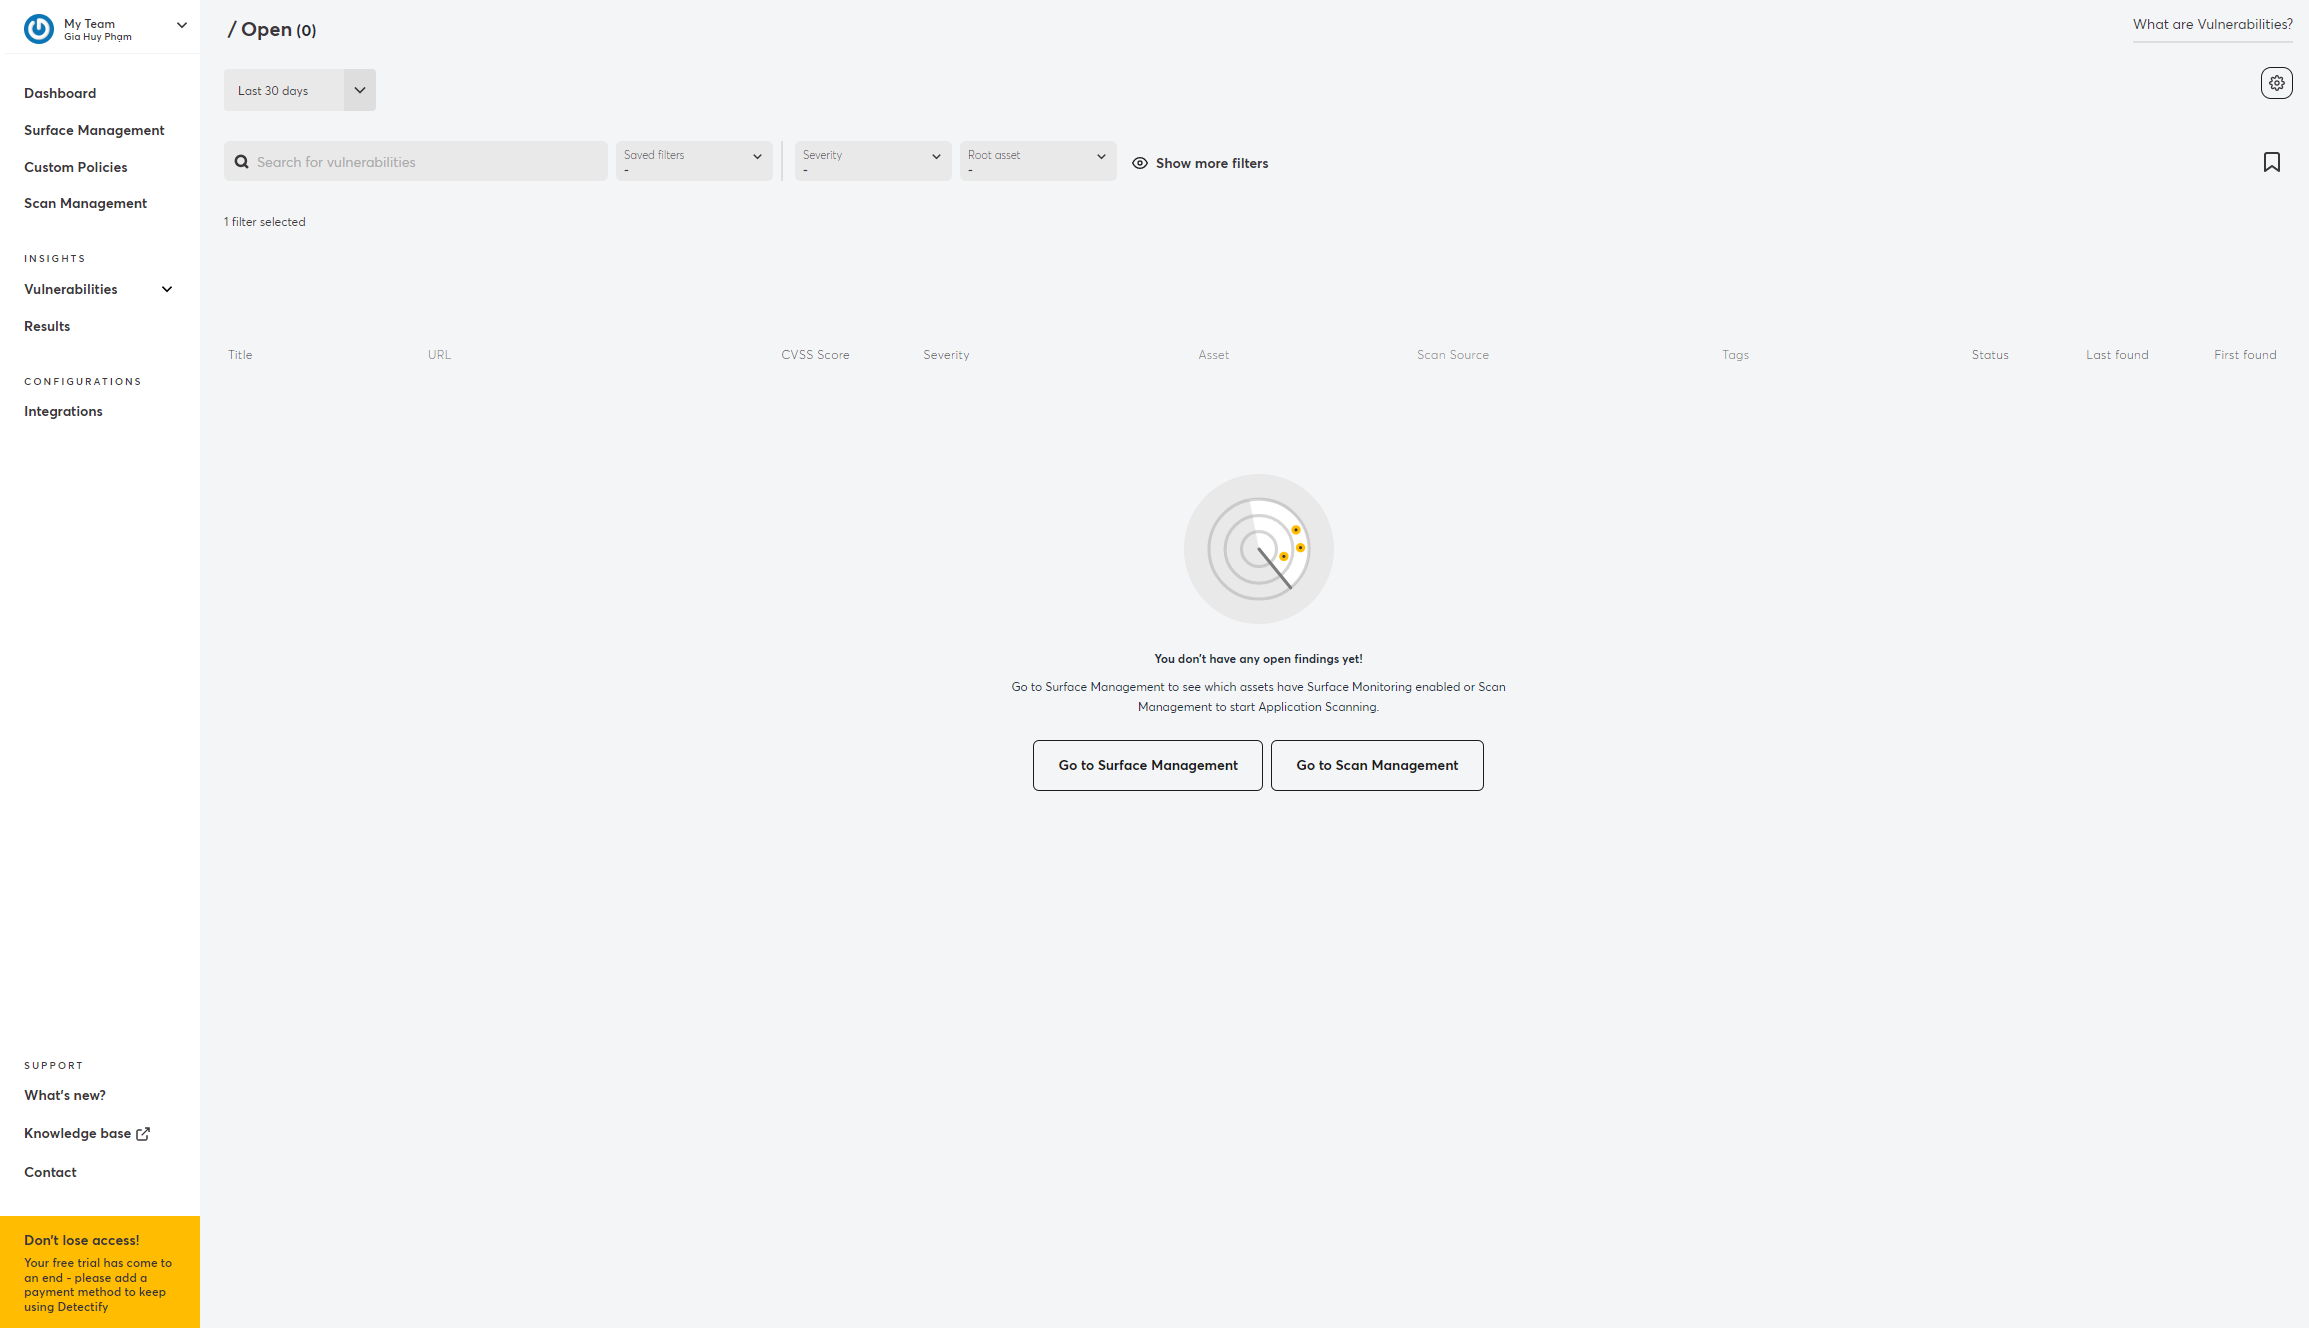
\includegraphics[width=\textwidth]{applied-thesis-chapters/chapter-1/detectify.com_app_vulnerabilities.png}
    \caption{Màn hình sau khi đăng nhập hệ thống Detectify}
\end{figure}

\newpage
\subsection{“StackHawk” do StackHawk Inc. phát triển}

\tab Được thành lập vào năm 2019 tại Mỹ.
Nền tảng cung cấp chức năng tìm lỗ hổng các ứng dụng dựa trên OWASP ZAP.
Nền tảng cung cấp các chức năng quản lý như tự động quét trên mỗi PR, cung cấp tài liệu hỗ trợ sửa lỗi tìm được tương ứng, tương tác được với nhiều ứng dụng, hệ thống khác như quản lý mã, quản lý dự án, quản lý lỗi, thông báo, tự động.
Nền tảng cung cấp đầy đủ các bản mã mẫu hướng dẫn sử dụng, tài liệu thông tin và hướng dẫn.
Đồng thời cũng có hỗ trợ trực tiếp cho ứng dụng OWASP ZAP.

\begin{figure}[H]
    \centering
    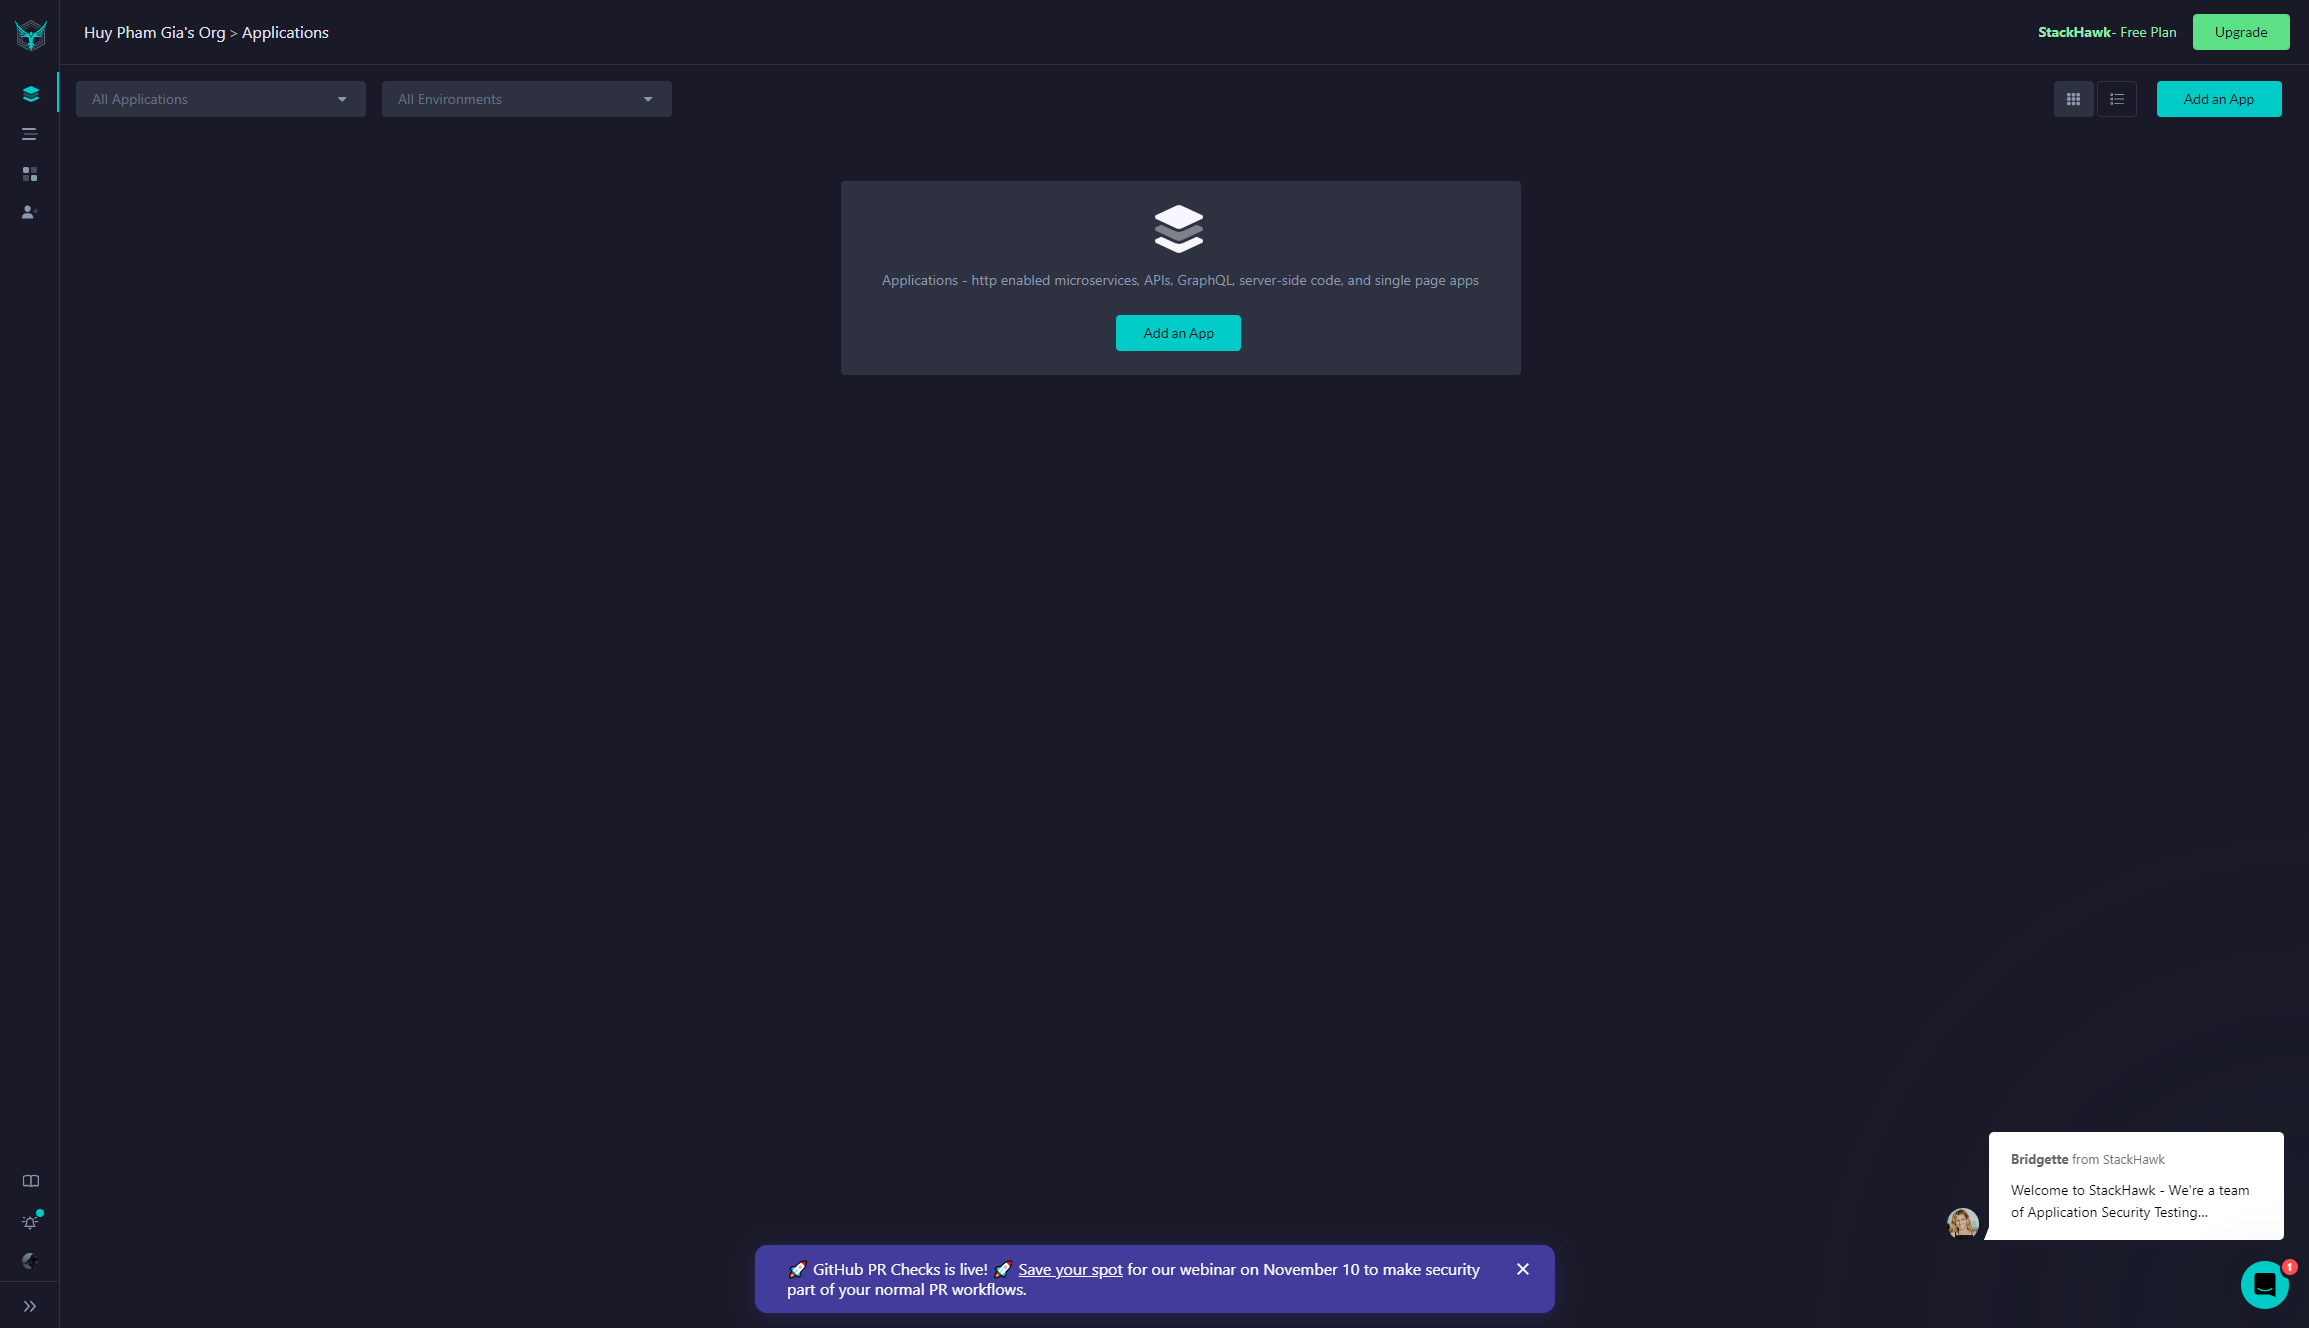
\includegraphics[width=\textwidth]{applied-thesis-chapters/chapter-1/app.stackhawk.com_applications.png}
    \caption{Màn hình sau khi đăng nhập hệ thống StackHawk}
\end{figure}

\newpage
\subsection{“HostedScan Security” do HostedScan LLC phát triển}

\tab Được thành lập vào năm 2019 tại Mỹ.
Nền tảng cung cấp nhiều loại quét như OWASP ZAP, Nmap, SSLyze.
Nền tảng có API riêng hỗ trợ cho việc sử dụng, nhúng các chức năng của nền tảng vào các ứng dụng, nền tảng khác.
Hỗ trợ hẹn lịch quét, báo cáo đầy đủ thông tin chi tiết và các tác vụ thông báo, tương tác qua email nhanh chóng.

\begin{figure}[H]
    \centering
    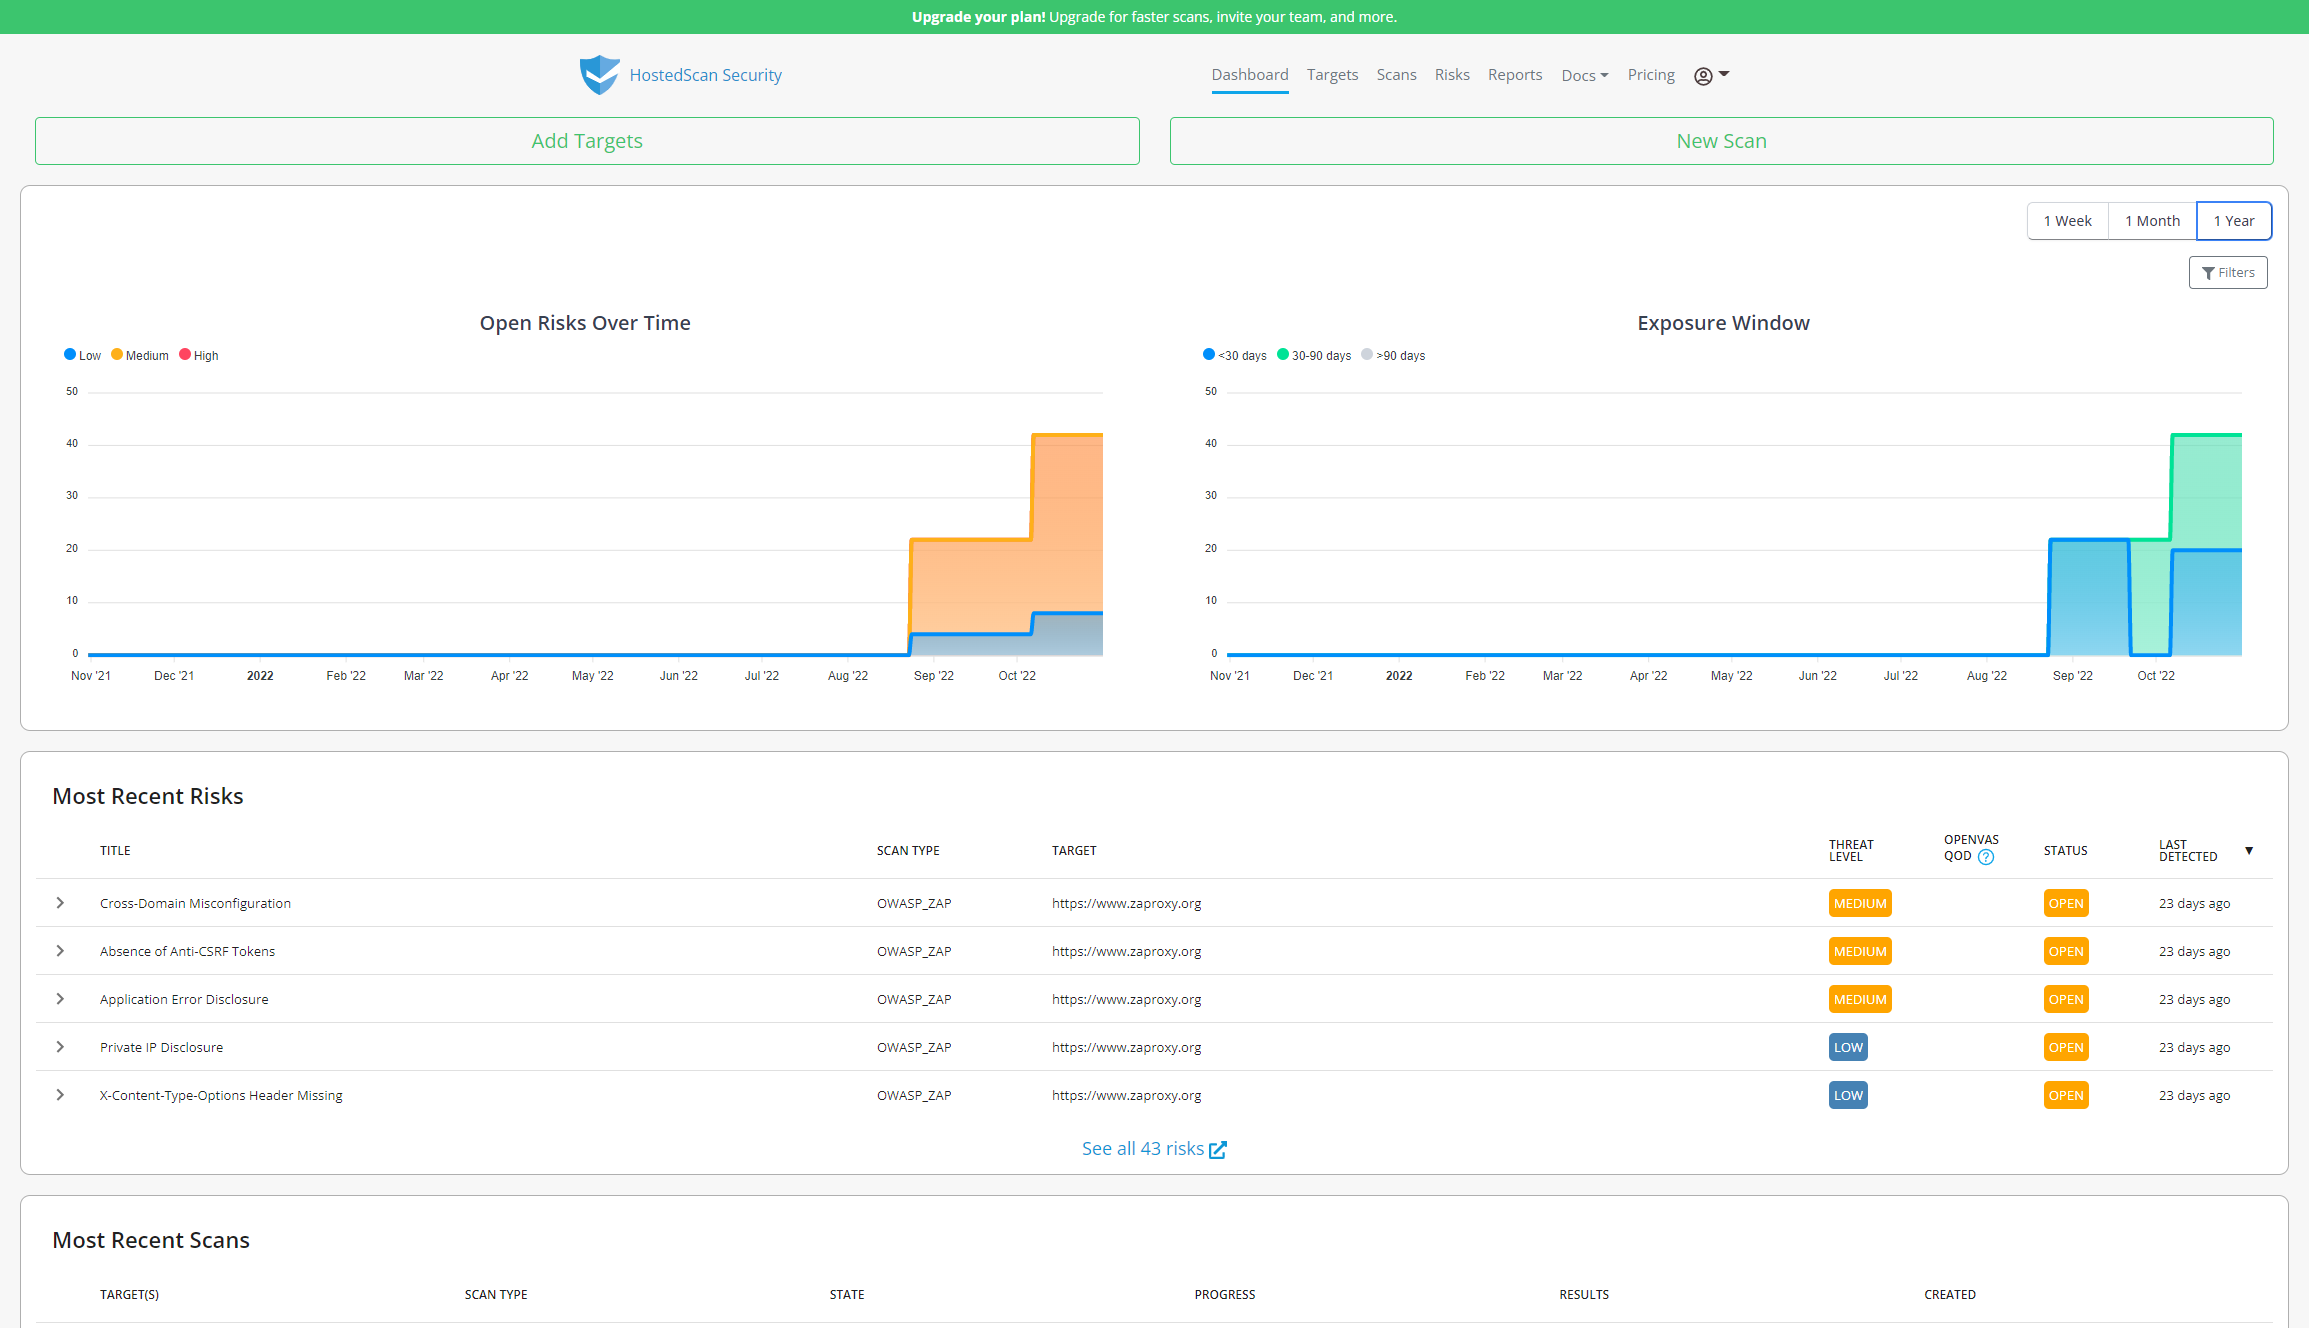
\includegraphics[width=\textwidth]{applied-thesis-chapters/chapter-1/hostedscan.com_dashboard.png}
    \caption{Màn hình sau khi đăng nhập hệ thống HostedScan Security}
\end{figure}

\newpage
\subsection{So sánh nhận xét 3 hệ thống}

\begin{tabularx}{\textwidth}{|>{\hsize=0.2\hsize\centering\let\newline
    \\\arraybackslash}X|>{\hsize=0.4\hsize\raggedright\let\newline
    \\\arraybackslash}X|>{\hsize=0.4\hsize\raggedright\let\newline
    \\\arraybackslash}X|}
    \hline
    \thead{Hệ thống}
     &
    \thead{Ưu điểm}
     &
    \thead{Chưa hoàn thiện}
    \\
    \hline
    Stack Hawk
     &
    - Tự động quét trên mỗi PR hoặc trong CI/CD.
    \newlinecontenttable
    - Quản lý thông tin kết quả quét, giao diện tường minh, dễ sử dụng.
    \newlinecontenttable
    - Đề xuất liên kết chứa thông tin sửa lỗi tìm được.
    \newlinecontenttable
    - Tích hợp được với những công cụ quản lý khác có sử dụng CI/CD như: Jira Sotfware, Gitlab, Github Action, Azure Pinelines, Jenkins, Travis CI,\dots
    \newlinecontenttable
    - Tài liệu hướng dẫn đầy đủ, chi tiết.
     &
    - Cần cấu hình pineline (.yml, .yaml).
    \newlinecontenttable
    - Cần Docker image đã build xây dựng sẵn.
    \newlinecontenttable
    - Kích hoạt quét bằng command line ở máy local. Cấu hình kích hoạt quét gồm nhiều bước.
    \newlinecontenttable
    - Dùng thử một lần mỗi ngày.
    \\
    \hline
    Hosted Scan
     &
    - Hỗ trợ các loại quét khác như Nmap, OpenVas, SSL/TLS.
    \newlinecontenttable
    - Hẹn thời gian đặt lịch quét.
    \newlinecontenttable
    - Đề xuất liên kết chứa thông tin sửa lỗi tìm được.
    \newlinecontenttable
    - Thông tin scan đầy đủ. Giao diện đơn giản.
     &
    - Kết quả scan dường như là dữ liệu gốc, không được xử lý.
    \newlinecontenttable
    - Dùng thử 10 lần mỗi tháng.
    \\
    \hline
    Detectify
     &
    - Tích hợp với các công cụ khác như: Slack, Jira, Zapier,…
    \newlinecontenttable
    - Đề xuất liên kết chứa thông tin sửa lỗi tìm được.
     &
    - Chi phí sử dụng cao.
    \newlinecontenttable
    - Cần phải cấu hình bên trong ứng dụng và triển khai để xác nhận chính chủ phức tạp, có thể không thành công.
    \newlinecontenttable
    - Không theo dõi được quá trình, tiến độ quét.
    \\
    \hline
    \caption{Bảng đánh giá chức năng giữa các hệ thống}\label{dummy-1}\\
\end{tabularx}


\section{Lý do lựa chọn đề tài}

\tab Trong thời đại ngày nay, các ứng dụng web phát triển với tốc độ nhanh chóng với số lượng, chất lượng và kích thước.
Tuy nhiên, điều này cũng làm tăng nguy cơ lỗ hổng bảo mật bị khai thác, phát hiện và lợi dụng nhiều hơn.
Gây ra nhiều nguy cơ tiềm ẩn cho ứng dụng, đội ngũ phát triển, đơn vị quản lý và chính bản thân người sử dụng ứng dụng.
Vì thế, việc tìm kiếm và khắc phục các lỗ hổng bảo mật trở thành thách thức không nhỏ, đặc biệt đối với các ứng dụng vừa và nhỏ.
\par

Mặc dù trên thị trường đã xuất hiện nhiều công cụ hỗ trợ kiểm tra, phát hiện và khắc phục lỗ hổng bảo mật cho ứng
dụng web, tuy nhiên các công cụ này thường yêu cầu nhiều bước cài đặt phức tạp hoặc chi phí sử dụng cao, khiến cho nhiều người dùng gặp khó khăn trong việc tiếp cận và sử dụng.
\par

Do đó, nhóm chúng em muốn tạo ra một hệ thống tự động tìm kiếm lỗi bảo mật ứng dụng web dựa trên nền tảng ZAP để hỗ trợ việc tìm kiếm và sửa chữa các lỗ hổng bảo mật dễ dàng hơn.
Nhắm đến kết quả tạo ra một hệ thống dễ dàng sử dụng, dễ tiếp cận và nhanh chóng.

\newpage
\section{Mục tiêu thực hiện}

Nhóm chúng em xác định rõ các mục tiêu cần đạt được khi thực hiện luận văn như sau:

\begin{itemize}
    \item Trình bày lý do xây dựng hệ thống tự động tìm kiếm lỗi bảo mật ứng dụng web dựa trên nền tảng OWASP ZAP.
    \item Trình bày các tính năng cơ bản của 3 ứng dụng tìm kiếm lỗi bảo mật ứng dụng web hiện có và nêu ra các khuyết điểm của các ứng dụng.
    \item Trình bày tóm tắt thông tin về các lỗi bảo mật ứng dụng web thường gặp.
    \item Xây dựng ứng dụng web tự động tìm kiếm lỗi bảo mật ứng dụng web với các chức năng:
          \begin{itemize}
              \item Quản lý tài khoản, các mục tiêu quét và kết quả quét.
              \item Quét các lỗi bảo mật với ZAP.
          \end{itemize}
    \item Viết 100 trang luận văn theo luồng logic trình bày trong tài liệu “Hướng dẫn thực hiện luận văn” mà giáo viên cung cấp, theo đúng chuẩn nhà trường yêu cầu và trích dẫn tài liệu tham khảo một cách chi tiết, đầy đủ.
\end{itemize}

\section{Phạm vi đề tài}

\tab Mục tiêu chính của đề tài “Hệ thống tự động tìm kiếm lỗi bảo mật ứng dụng web dựa trên nền tảng OWASP ZAP” là hướng tới sự dễ dàng và nhanh chóng tìm kiếm lỗi bảo mật ứng dụng và quản lý kết quả sau khi quét.
Vì vậy ứng dụng sẽ chú trọng phát triển các tính năng quét chính với ZAP đã đề xuất.
Và các chức năng quản lý cơ bản của nền tảng như quản lý mục tiêu, quản lý phiên quét.
Tuy vậy, ứng dụng sẽ tập trung vào trực quan hóa quá trình quét và giảm thiểu các cấu hình bắt buộc khi bắt đầu một phiên quét.
\chapter{CƠ SỞ LÝ THUYẾT}

\section{Các loại lỗi bảo mật phổ biến}

\subsection{Lỗ hổng kiểm soát truy cập - Broken Access Control ~\cite{chap2bib1}}
 
\paragraph{Khái niệm}

\begin{itemize}
    \item Access Control - Kiểm soát truy cập là việc kiểm soát quyền truy cập, thực hiện hành vi của người dùng trong phạm vi đã được dự định, cấp sẵn trước đó.
    \item Broken Access Control - Lỗ hổng kiểm soát truy cập là lỗ hỗng bị lợi dụng bằng những phương thức tấn công như xâm nhập, chiếm quyền sử dụng, kiểm soát các tài nguyên được bảo vệ trên hệ thống một cách trái phép. Việc này thường gây ra các hệ quả như để lộ, bị can thiệp sửa đổi thông tin một cách không mong muốn, bị phá hoại dữ liệu và thực hiện các chức năng bên ngoài phạm vi của quyền người dùng.
    \item Các CWE đáng chú ý bao gồm: CWE-200: Exposure of Sensitive Information to an Unauthorized Actor ~\cite{chap2bib4}, CWE-201: Insertion of Sensitive Information Into Sent Data ~\cite{chap2bib5}, và CWE-352: Cross-Site Request Forgery ~\cite{chap2bib6}.
\end{itemize}

\paragraph{Các lỗi thường gặp trong Broken Access Control}

\begin{itemize}
    \item Vi phạm cấu hình về đặc quyền tối thiểu. Quyền truy cập chỉ nên được cấp cho từng khả năng, nhu cầu, quyền và người dùng cụ thể thay vì cấp chung cho tất cả mọi người hoặc có những tồn tại không cần thiết.
    \begin{figure}[H]
        \centering
        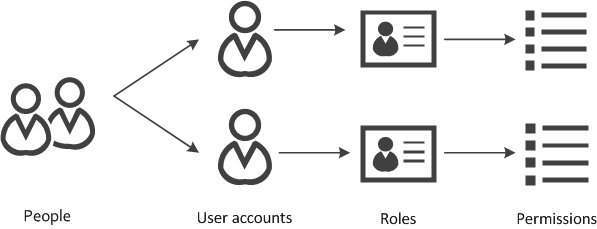
\includegraphics[width=\textwidth]{applied-thesis-chapters/chapter-2/Nguyên tắc đặc quyền tối thiểu.png}
        \caption{Nguyên tắc đặc quyền tối thiểu.png ~\cite{chap2bib2}}
    \end{figure}
    \item Có thể vượt qua phần kiểm tra quyền truy cập bằng các thao tác như mạo danh tham chiếu (Parameter Tampering) hoặc đường dẫn (Force Browsing) trong URL, thay đổi trạng thái ứng dụng và thay đổi nội dung các API gửi đi.
    \item Tham chiếu đối tượng không an toàn (Insecure Direct Object Reference - IDOR). Đối tượng có thể được tham chiếu qua nhiều phương pháp, tuy nhiên định danh duy nhất của đối tượng dùng để tham chiếu lại quá dễ đoán, không được tiền xử lý
    Như hình \ref{fib:DuLieuNhayCam} mô tả.
    \begin{figure}[H]
        \centering
        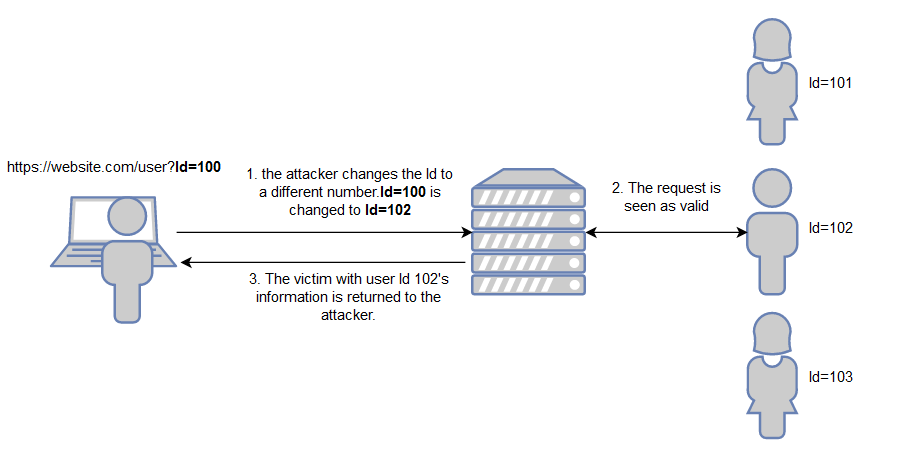
\includegraphics[width=\textwidth]{applied-thesis-chapters/chapter-2/Mô tả dữ liệu nhạy cảm có thể được tìm thấy trong URL.png}
        \caption{Mô tả dữ liệu nhạy cảm có thể được tìm thấy trong URL ~\cite{chap2bib3}}
        \label{fib:DuLieuNhayCam}
    \end{figure}
    \item Các truy cập API không phân biệt rõ ràng hoặc không cấu hình các phương thức GET, POST, PUT, DELETE,…
    \item Lổ hỗng Nâng cao Đặc quyền - Elevation of Privilege. Lỗ hổng này đề cập đến việc người dùng có thể bằng cách nào đó thay đổi đặc quyền của mình đối với hệ thống một cách không chính thống.
    \item Cấu hình sai CORS, cho phép gửi API từ các nguồn không tin tưởng, không được cấp quyền.
\end{itemize}

\paragraph{Cách phòng tránh}

\begin{itemize}
    \item Thiết kế một cơ chế access control và sử dụng xuyên suốt ứng dụng, hạn chế tối đa sử dụng Cross-Origin Resource Sharing (CORS).
    \item Trong mô hình access controls, các bản ghi trong cơ sở dữ liệu nên có quyền sở hữu và chỉ những ai có quyền sở hữu có thể thêm, xoá, sửa bản ghi đó.
    \item Không cho phép duyệt file trên Web Server, bảo đảm rằng các file metadata (e.g., .git) file backup không được nằm trong Web Root.
    \item Lưu lại các lỗi về access control, thông báo cho admin nếu cần thiết.
    \item Các phiên làm việc lưu tại Server phải được huỷ khi người dùng đăng xuất. JWT token nên có thời hạn ngắn.
\end{itemize}

\subsection{Cryptographic Failures ~\cite{chap2bib7}}

\paragraph{Khái niệm ~\cite{chap2bib8}}

\begin{itemize}
    \item Cryptographic failure là một lỗi bảo mật nghiêm trọng của ứng dụng web, đó là để lộ thông tin nhạy cảm bằng những thuật toán mã hoá yếu hoặc không mã hoá dữ liệu. Những thông tin này có thể bao gồm mật khẩu, hồ sơ sức khoẻ bệnh nhân, thông tin bí mật doanh nghiệp, thông tin thẻ thanh toán, địa chỉ email, … và các thông tin cá nhân khác.
    \item Ngoài việc để lộ thông tin nhạy cảm, sự cố trong các hệ thống mật mã hóa cũng tạo ra lỗ hổng trong hệ thống. Đây được coi là một trong những rủi ro bảo mật quan trọng nhất đối với cả tổ chức và các người dùng kinh doanh.
    \item Các CWE đáng chú ý bao gồm: CWE-259: Use of Hard-coded Password ~\cite{chap2bib9}, CWE-327: Broken or Risky Crypto Algorithm ~\cite{chap2bib10}, và CWE-331 Insufficient Entropy ~\cite{chap2bib11}.
\end{itemize}

\myparagraph{Các lỗi thường gặp trong Cryptographic Failures}
\tab \tab Trước tiên, ta cần xác định mức độ “cần bảo vệ” của dữ liệu ở cả trạng thái truyền đi hoặc không. Các dữ liệu như mật khẩu, số thẻ tín dụng, hồ sơ y tế, thông tin cá nhân và bí mật kinh doanh đòi hỏi nhiều sự bảo mật, đặc biệt nếu dữ liệu đó nằm trong phạm vi của các luật về quyền riêng tư, ví dụ như Nghị định bảo vệ dữ liệu chung châu Âu (GDPR) hoặc các quy định về bảo vệ dữ liệu tài chính như Tiêu chuẩn bảo mật dữ liệu PCI (PCI DSS). Đối với các dữ liệu đó, ta cần đảm bảo không mắc phải các lỗi bảo mật:

\begin{itemize}
    \item Kiểm tra xem có dữ liệu nào được truyền dưới dạng văn bản không mã hoá (clear text) không, đặc biệt khi có liên quan đến các giao thức như HTTP, SMTP, hay FTP sử dụng cải tiến TLS như STARTTLS. Cần nhớ rằng lưu lượng internet từ bên ngoài có rất nhiều rủi ro. Lưu lượng nội bộ cũng cần được đảm bảo tính bảo mật, ví dụ như giữa các bộ cân bằng tải (load balancers), các máy chủ web hoặc các hệ thống back-end.
    \item Liệu có bất cứ một thuật toán hoặc giao thức mật mã cũ hoặc yếu nào được sử dụng trong cài đặt mặc định hoặc trong mã nguồn cũ không?
    \item Liệu có bất kì đâu trong hệ thống mà mã hóa chưa được tận dụng, như là thiếu chỉ thị bảo mật của các HTTP header (trình duyệt) hoặc thiếu các header tương ứng?
    \item Liệu thuật toán ngẫu nhiên dùng cho mục đích mã hóa không được thiết kế để đáp ứng yêu cầu? Ngay cả khi đã chọn được thuật toán chính xác, liệu nó cần được khởi tạo (seed) thủ công, và nếu không thì liệu ta có đang ghi đè chức năng khởi tạo tối ưu hơn vốn được tích hợp sẵn, và seed của ta thì không đáp ứng các yếu tố entropy/unpredictability?
    \item Liệu ta có đang sử dụng các hàm băm đã lỗi thời như MD5 hoặc SHA1, hoặc các hàm băm không có tính chất mật mã trong những trường hợp cần mã hóa không?
\end{itemize}

\paragraph{Cách phòng tránh}

\begin{itemize}
    \item Phân loại các dữ liệu được lưu trữ, truyền qua hoặc xử lí trong hệ thống. Xác định các dữ liệu nhạy cảm theo các luật về quyền riêng tư, các quy định hoặc theo nhu cầu kinh doanh.
    \item Hạn chế lưu trữ dữ liệu nhạy cảm. Loại bỏ các dữ liệu này ngay khi có thể hoặc sử dụng tokenization theo chuẩn PCI DSS, hay thậm chí là cắt bớt dữ liệu. Dữ liệu không được lưu trữ thì sẽ không bị đánh cắp.
    Tokenization là quá trình thay thế dữ liệu nhạy cảm bằng một mã thông báo (token) không thể đoán được và không có giá trị thực.
    \item Đảm bảo mã hóa tất cả dữ liệu nhạy cảm cho dù đang không được truyền đi.
    \item Đảm bảo sử dụng các thuật toán, giao thức và khóa tiêu chuẩn hiện đại; đảm bảo quản lý khóa (key management) đúng cách.
    \item Mã hóa tất cả dữ liệu trong đang truyền với các giao thức an toàn (secure protocols) như TLS với phương pháp mã hoá forward secrecy (FS), ưu tiên mã hoá (cipher prioritization) bởi máy chủ và các tham số an toàn (secure parameters). Áp dụng mã hóa bằng cách sử dụng chỉ thị như HTTP Strict Transport Security (HSTS).
    \item Tắt bộ nhớ cache với các phản hồi (response) chứa dữ liệu nhạy cảm.
    \item Áp dụng các phương pháp bảo mật theo nhu cầu của từng loại dữ liệu.
    \item Không sử dụng các giao thức lỗi thời như FTP và SMTP để truyền dữ liệu nhạy cảm.
    \item Lưu trữ mật khẩu với các hàm băm mạnh mẽ như Argon2, scrypt, bcrypt hoặc PBKDF2.
    \item Đảm bảo tính ngẫu nhiên trong mật mã hóa được dùng khi cần thiết và không được khởi tạo (seed) một cách dễ đoán hoặc có entropy thấp. Hầu hết các API hiện đại đều không yêu cầu khởi tạo thủ công CSPRNG.
    \item Tránh sử dụng các thuật toán mã hóa đã lỗi thời, chẳng hạn như MD5, SHA1, PKCS số 1 v1.5.
\end{itemize}

\subsection{Injection ~\cite{chap2bib12}}

\paragraph{Khái niệm ~\cite{chap2bib13}}

\begin{itemize}
    \item Kẻ tấn công gửi dữ liệu không hợp lệ đến một ứng dụng web để khiến nó thực hiện những hành động không được thiết kế/lập trình sẵn.
    \item Khi cung cấp dữ liệu hoặc câu lệnh xấu cho một trình thông dịch (interpreter) như một phần của lệnh hoặc truy vấn, trình thông dịch sẽ bị lừa để thực thi các lệnh không mong muốn hoặc truy cập dữ liệu mà không có sự cho phép.
    \item Một số phương pháp injection phổ biến bao gồm SQL Injection, NoSQL Injection, Object Relational Mapping (ORM), LDAP và Expression Language (EL) hoặc Object Graph Navigation Library (OGNL).
    \item Các CWE đáng chú ý bao gồm: CWE-79: Cross-site Scripting ~\cite{chap2bib14}, CWE-89: SQL Injection ~\cite{chap2bib15} và CWE-73: External Control of File Name or Path ~\cite{chap2bib16}.
\end{itemize}

\paragraph{Các lỗi thường gặp trong Injection}

\begin{itemize}
    \item Do dữ liệu người dùng cung cấp không được xác thực, lọc (filtered) hoặc làm sạch (sanitized).
    \item Dùng trực tiếp các truy vấn động hoặc các non-parameterized call mà không có cơ chế context-aware escaping trong trình thông dịch.
    \item Dữ liệu độc hại được sử dụng trong các tham số tìm kiếm của object-relational mapping (ORM) để truy cập các bản ghi nhạy cảm.
    \item Câu lệnh SQL hoặc lệnh chứa cấu trúc và dữ liệu độc hại trong các truy vấn động, lệnh hoặc các thủ tục được lưu sẵn (stored procedures).
\end{itemize}

\myparagraph{Cách phòng tránh}

\tab \tab Để ngăn chặn injection, ta cần tách riêng dữ liệu khỏi các lệnh và truy vấn.

\begin{itemize}
    \item Kiểm thử tự động cho tất cả các tham số, headers, URL, cookie, JSON, SOAP và đầu vào dữ liệu XML.
    \item Có thể tích hợp các công cụ kiểm thử bảo mật ứng dụng tĩnh (SAST), động (DAST) và tương tác (IAST) vào quy trình CI/CD để xác định các lỗi injection trước khi triển khai vào môi trường production.
    \item Ưu tiên thiết kế và sử dụng API an toàn. Một API an toàn sẽ giúp ta tránh sử dụng trình thông dịch và cung cấp ta giao diện có tham số (parameterized interface). Ta cũng có thể chuyển sang sử dụng các công cụ Object Relational Mapping (ORMs).
    \par
    Lưu ý: Ngay cả khi có tham số, các thủ tục được lưu sẵn (stored procedures) vẫn có thể tạo ra lỗi SQL injection nếu PL/SQL hoặc T-SQL nối các truy vấn và dữ liệu hoặc thực thi dữ liệu độc hại bằng lệnh EXECUTE IMMEDIATE hoặc exec().
    \item Sử dụng xác thực đầu vào tích cực phía máy chủ (positive server-side input validation). Tuy nhiên, đây không phải là một biện pháp phòng thủ hoàn chỉnh vì nhiều ứng dụng vẫn cần sử dụng các ký tự đặc biệt, chẳng hạn như trong văn bản hoặc API cho ứng dụng di động.
    \item Đối với các truy vấn động còn lại, nên tránh các ký tự đặc biệt bằng cách escape các kí tự, tham số cụ thể cho trình thông dịch đó.
    \item Sử dụng các cách điều khiển SQL (SQL controls) trong các truy vấn như LIMIT để ngăn chặn việc để lộ hàng loạt bản ghi trong trường hợp bị SQL injection.
\end{itemize}

\subsection{Insecure Design ~\cite{chap2bib17}}

\paragraph{Khái niệm ~\cite{chap2bib18}}

\begin{itemize}
    \item Khi thiết kế ứng dụng, nhà phát triển được khuyến nghị sử dụng các design pattern an toàn, tiến hành mô hình hóa mối đe dọa (threat modeling) một cách cẩn thận và tham khảo các kiến trúc mẫu để giúp ứng dụng tránh các lỗ hổng bảo mật.
    \item Các security controls thiếu hiệu quả trong giai đoạn thiết kế thường dẫn nhiều lỗ hổng trong ứng dụng. Lỗi này thường được biết đến với tên gọi insecure design vulnerabilities.
    \item Ngoài ra, thiết kế thiếu an toàn (insecure design) còn có các rủi ro bắt nguồn từ việc bỏ qua các quy tắc thiết kế và kiến trúc được khuyên dùng. Lỗi này thường bắt đầu từ giai đoạn lập kế hoạch trước khi bước vào giai đoạn implementation.
    \item Các CWE đáng chú ý bao gồm: CWE-209: Generation of Error Message Containing Sensitive Information ~\cite{chap2bib19}, CWE-256: Unprotected Storage of Credentials ~\cite{chap2bib20}, CWE-501: Trust Boundary Violation ~\cite{chap2bib21}, và CWE-522: Insufficiently Protected Credentials ~\cite{chap2bib22}.
\end{itemize}

\paragraph{Các lỗi thường gặp trong Insecure Design ~\cite{chap2bib18}}

\begin{itemize}
    \item Trust boundary violations: xảy ra khi interface chấp nhận và lưu trữ cả dữ liệu đáng tin cậy và dữ liệu không đáng tin cậy trong cùng một kho lưu trữ dữ liệu. Nhà phát triển thường không phân ra giữa nguồn dữ liệu đáng tin cậy và không đáng tin cậy, đẫn đến việc các dữ liệu và lệnh độc hại được truyền vào ứng dụng.
    \item Thông báo lỗi dài dòng và chứa thông tin nhạy cảm như ID người dùng, mật khẩu, môi trường ứng dụng hoặc dữ liệu liên quan khác mà kẻ tấn công có thể lợi dụng.
    \item Improper isolation: xảy ra khi ứng dụng không tách ra được các thực thể (entities) với các quyền (rights), đặc quyền (privileges) và quyền truy cập (access permissions) khác nhau. Điều này dẫn đến việc kiểm soát truy cập bị hỏng (broken access control).
\end{itemize}

\paragraph{Cách phòng tránh}

\begin{itemize}
    \item Thiết lập và sử dụng một quy trình phát triển (development lifecycle) an toàn với các chuyên gia AppSec để giúp đánh giá và thiết kế các điều khiển (controls) về bảo mật và riêng tư.
    \item Thiết lập và sử dụng thư viện với các design pattern an toàn hoặc các component đã được thiết lập hoàn chỉnh để sử dụng.
    \item Sử dụng threat modeling cho các thao tác xác thực quan trọng, kiểm soát truy cập, logic kinh doanh và các luồng chính (key flows).
    Threat modeling là một kỹ thuật được sử dụng trong lĩnh vực bảo mật thông tin để đánh giá và phân tích các mối đe dọa tiềm năng đến hệ thống, ứng dụng hoặc sản phẩm.
    \item Tiến hành kiểm tra tính hợp lý ở từng tầng (tier) của ứng dụng (từ frontend đến backend).
    \item Viết unit test và integration để chắc chắn rằng tất cả các luồng quan trọng đều chống lại được threat model đã đặt ra. Tổng hợp các use-case và misuse-case cho từng tầng của ứng dụng.
    \item Phân tách các lớp (layer) của tầng theo lớp hệ thống và lớp mạng dựa trên mức độ tiếp xúc với bên ngoài (exposure) và nhu cầu được bảo vệ của nó.
    \item Phân tách khách hàng từ khâu thiết kế trong tất cả các tầng.
    \item Giới hạn khả năng sử dụng tài nguyên theo người dùng hoặc theo dịch vụ.
\end{itemize}

\subsection{Security Misconfiguration ~\cite{chap2bib23}}

\paragraph{Khái niệm}

\begin{itemize}
    \item Các mạng (network) hiện đại bao gồm nhiều loại thiết bị mạng, máy chủ và dịch vụ. Từng loại này cần được cấu hình và giám sát để đảm bảo luôn tuân thủ các chính sách bảo mật đã đề ra.
    \item Lỗi cấu hình bảo mật (security misconfiguration) xảy ra khi các tùy chọn bảo mật đã cài đặt không tối đa hóa bảo mật, hoặc khi các dịch vụ được triển khai với cài đặt mặc định thiếu an toàn.
    \item Các framework giúp việc lập trình dễ dàng hơn, giảm thời gian và công sức xây dựng ứng dụng. Tuy nhiên, các framework này thường có cấu hình phức tạp, làm tăng nguy cơ xảy ra lỗi cấu hình bảo mật. Tương tự, sử dụng mã nguồn mở có thể đi kèm với cấu hình mặc định, đe dọa tính bảo mật của ứng dụng.
    \item Các CWE đáng chú ý bao gồm: CWE-16 Configuration ~\cite{chap2bib24} và CWE-611 Improper Restriction of XML External Entity Reference ~\cite{chap2bib25}.
\end{itemize}

\paragraph{Các lỗi thường gặp trong Security Misconfiguration}

\begin{itemize}
    \item Không gia cố bảo mật (security hardening) một cách phù hợp trong ứng dụng hoặc phân quyền không hợp lí trên dịch vụ đám mây.
    \item Các tính năng không cần thiết lại được bật hoặc cài đặt (ví dụ: cổng, dịch vụ, trang, tài khoản hoặc đặc quyền không cần thiết).
    \item Xử lý lỗi (error handling) làm lộ các stack trace hoặc lỗi được thông báo với quá nhiều thông tin cho người dùng.
    \item Với các hệ thống đã được nâng cấp, các tính năng bảo mật mới nhất lại bị vô hiệu hoá hoặc không được cấu hình một cách an toàn.
    \item Các cài đặt bảo mật trong các máy chủ ứng dụng, các framework ứng dụng (ví dụ: Struts, Spring), thư viện, cơ sở dữ liệu, ... không được cài đặt với các thiết lập an toàn.
    \item Máy chủ không gửi các header hoặc chỉ thị bảo mật, hoặc chúng không được cài đặt với các giá trị an toàn.
    \item Phần mềm đã lỗi thời hoặc có lỗ hổng bảo mật.
\end{itemize}

\paragraph{Cách phòng tránh}

\begin{itemize}
    \item Môi trường phát triển, QA và production nên được cấu hình giống nhau, với các thông tin đăng nhập khác nhau cho mỗi môi trường. Quá trình này nên được tự động hóa để giảm thiểu công sức thiết lập môi trường mới một cách an toàn.
    \item Tạo một nền tảng tối giản mà không có các tính năng, component, documentation và sample không cần thiết. Loại bỏ các tính năng và framework không sử dụng.
    \item Đặt ra task để xem xét và cập nhật các cấu hình phù hợp với tất cả các note, cập nhật và bản vá bảo mật trong quá trình quản lý vá lỗi.
    \item Kiểm tra quyền lưu trữ đám mây (ví dụ: quyền bucket S3).
    \item Dùng kiến trúc ứng dụng phân đoạn (segmented application architecture) để phân tách một cách hiệu quả và an toàn giữa các component hoặc các khách hàng, với việc phân đoạn (segmentation), đóng gói (containerization) hoặc các nhóm bảo mật đám mây (cloud security groups  hay ACLs).
    \item Gửi các chỉ thị bảo mật tới khách hàng, ví dụ: header bảo mật (security headers).
    \item Tự động hóa quy trình để xác minh tính hiệu quả của các cấu hình và thiết lập trong tất cả môi trường.
\end{itemize}

\section{Kiến trúc phân tầng (N-Tier)} \label{sec:NTier}

\paragraph{Giới thiệu giải pháp ~\cite{chap2bib26} ~\cite{chap2bib27}}

\begin{itemize}
    \item Kiến trúc phân tầng phân chia ứng dụng thành nhiều tầng xếp chồng, trong đó mỗi tầng có nhiệm vụ, chức năng độc lập nhau và tự quản lý các tài nguyên của mình. Kiến trúc hoạt động theo nguyên lý tầng phía có thể gửi yêu cầu, sử dụng các chức năng của tầng kế dưới và không có chiều ngược lại.
    \item Các tầng trong ứng dụng thường được phân tách nhau cả về mặt vật lý, mỗi tầng sẽ hoạt động trong một môi trường, tài nguyên, hệ thống riêng (mặc dù điều này không bắt buộc). 
    \item Việc phân chia các tầng về mặt vật lý, sẽ giúp tăng hiệu quả làm việc của hệ thống; giúp dễ dàng quản lý, nâng cấp và thay thế các tầng nhờ đã được module hoá, nhưng đồng thời khiến việc giao tiếp giữa các tầng kém hiệu quả và gây ra độ trễ không cần thiết.
    \item Các tầng có 2 cách giao tiếp
    \begin{itemize}
        \item Trực tiếp: thông qua HTTP request, Websocket, Pipeline,…
        \item Gián tiếp: thông qua hệ thống trung gian có nhiệm nhận và phân tán request (message queue).
    \end{itemize}
\end{itemize}

\paragraph{Ưu điểm}

\begin{itemize}
    \item Dễ dàng tiếp cận với đa số lập trình viên.
    \item Công việc kiểm thử và sửa lỗi sẽ dễ dàng hơn vì có thể thực hiện trên một tầng thay vì toàn bộ hệ thống.
    \item Hiệu suất sẽ tốt hơn nếu được triển khai hay cài đặt một cách có hệ thống, phù hợp. Về mặt độ trễ của phản hồi có thể vượt trội hơn khi được so sánh với kiến trúc Microservice có độ trễ nhất định trong giao tiếp giữa các service.
    \item Dễ dàng thay thế, nâng cấp hệ thống.
    \item Được hỗ trợ bởi các nền tảng Cloud hiện nay.
    \item Ứng dụng có thể hoạt động trên nhiều môi trường, hệ điều hành, công nghệ khác nhau.
\end{itemize}

\paragraph{Nhược điểm}

\begin{itemize}
    \item Khó khăn trong việc đảm bảo tương tác giữa các tầng và xử lý các vấn đề về hiệu suất. 
    \item Phức tạp hóa quy trình phát triển và triển khai do sự tách biệt giữa các tầng.
    \item Hệ thống IaaS (Cơ sở hạ tầng như Một Dịch vụ, hay Infrastructure as a Service) khó quản lý và cần nhiều thời gian tìm hiểu, học hỏi.
    \item Hệ thống càng phân tán càng tiềm ẩn nhiều nguy cơ bảo mật.
\end{itemize}

\newpage
\section{Kiến trúc nguồn sự kiện (Event Sourcing) \cite{chap2bib28} \cite{chap2bib29}}

\paragraph{Giới thiệu giải pháp}

\begin{itemize}
    \begin{figure}[H]
        \centering
        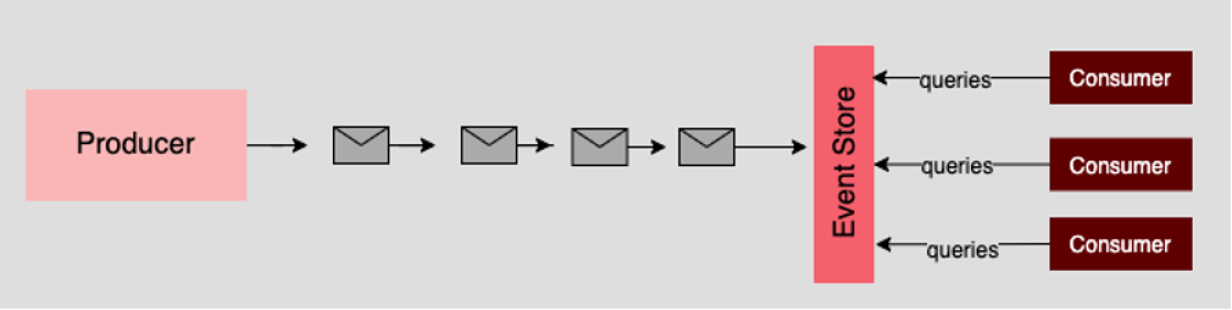
\includegraphics[width=\textwidth]{applied-thesis-chapters/chapter-2/Mẫu kiến trúc nguồn sự kiện.png}
        \caption{Mẫu kiến trúc nguồn sự kiện \cite{chap2bib29}}
    \end{figure}
    \item Nguồn sự kiện sẽ trả về các sự kiện theo thời gian xuất hiện (ở dạng stream). Những nơi cần sử dụng có thể đăng ký với nguồn sự kiện, sau đó sẽ được thông báo và có thể xử lý chúng nếu cần.
    \item Kiến trúc nguồn sự kiện đảm nhiệm công việc tạo ra và gửi đi các luồng tin nhắn liên tục đến một nơi lưu trữ. Mỗi tin nhắn mô tả một sự kiện trong hệ thống. Sau đó, các dịch vụ và ứng dụng khác sẽ truy vấn để tìm các sự kiện theo nhu cầu.
\end{itemize}

\paragraph{Ưu điểm}

\begin{itemize}
    \item Cực kỳ linh hoạt. Bất kỳ loại tin nhắn đều có thể được lưu trữ và truy xuất.
    \item Thích hợp cho tác vụ báo cáo dữ liệu theo thời gian thực.
    \item Các sự kiện là bất biến và chỉ có thể được thêm vào hệ thống lưu trữ. Các nơi cần sử dụng như giao diện người dùng hoặc tác vụ khởi tạo sự kiện có thể tiếp tục công viêc. Và các tác vụ xử lý sự kiện có thể chạy ở môi trường nền.
    \item Sự kiện chỉ là các đối tượng đơn giản mô tả một số hành động đã xảy ra, cùng với những dữ liệu liên quan. Chúng chỉ được ghi lại để xử lý vào thời điểm thích hợp khác. Sử dụng các sự kiện có thể đơn giản hóa việc triển khai và quản lý.
    \item Việc chỉ cho phép lưu trữ thêm các sự kiện mới cung cấp một lộ trình theo thời gian có thể được sử dụng để giám sát các hành động được thực hiện trong hệ thống. Danh sách các sự kiện cũng có thể được sử dụng để phân tích hiệu suất của ứng dụng.
\end{itemize}

\paragraph{Nhược điểm}

\begin{itemize}
    \item Các sự kiện khác nhau sẽ chứa các thông tin, định dạng khác nhau. Cần phải có một nguồn sự thật duy nhất để xác định và xác định định dạng thông báo cho một sự kiện cụ thể.
    \item Việc triển khai giải pháp nguồn sự kiện có thể đòi hỏi kiến thức chuyên môn và kỹ năng phát triển phần mềm cao.
\end{itemize}

\chapter{THIẾT KẾ GIẢI PHÁP}

\section{Giải pháp tổng quát} \label{sec:AbstractSol}

\tab Để có được một công cụ xác định lỗi bảo mật web bằng các phương pháp khác nhau sẽ là một vấn đề rất rộng, cần nhiều thời gian cũng như nguồn lực mới có thể phát triển, triển khai và bảo trì.
Vì vậy, trong phạm vi của khóa luận, nhóm chọn thiết kế giải pháp dựa trên công cụ OWASP Zed Attack Proxy - ZAP là một công cụ mã nguồn mở uy tín trong giới, có đội ngũ chuyên môn cao và hàng trăm nhà phát triển đang đóng góp đến nay.
Các giải pháp nhóm đưa ra như sau.

\subsection{Giải pháp quét lỗi bảo mật với ZAP}

\tab Việc sử dụng ứng dụng ZAP trực tiếp sẽ đòi hỏi nhiều yêu cầu cần thiết như phần cứng đáp ứng đủ điều kiện sử dụng ứng dụng, lựa chọn phiên bản phù hợp với cấu hình, tải xuống, cài đặt môi trường (Java Runtime Environment - JRE), xử lý lỗi cài đặt - cấu hình.
Nhiều hơn nữa, để sử dụng được một số chức năng, người dùng cần phải biết cách cấu hình trình duyệt cho ZAP, quản lý dữ liệu của phiên sử dụng, cấu hình cho phương thức và nhiều tác vụ khác.

Quét lỗi bảo mật web với ZAP là giải pháp, mục tiêu quan trọng và cốt lõi của hệ thống mà nhóm nhắm tới.
Với mục tiêu ban đầu là nhanh chóng, dễ sử dụng với mong muốn là dễ tiếp cận người dùng hơn thì các điều kiện đã nêu trên là vấn đề cần giải quyết.
Vì vậy, nhóm đề xuất giải pháp quét với 4 phương pháp có trong ZAP là Spider, Ajax Spider, Active và Passive là 4 phương pháp quét bảo mật web phổ biến và không cần sử dụng trực tiếp ứng dụng ZAP.

Khi sử dụng giải pháp được đề xuất ở trên, người dùng có thể tạo các phiên quét bằng cách cung cấp các địa chỉ URL hoặc IP trang web cần quét và chọn các phương pháp quét.
Từ đó hệ thống sẽ thực hiện quét các phiên này với ZAP và thu được kết quả quét tương ứng của từng địa chỉ với từng phương pháp quét đã chọn.
Kết quả quét sẽ được lưu trữ, quản lý và hiển thị cho người dùng.
Với các phương pháp quét với Spider thì người dùng có thể xem được quá trình quét trong thời gian thực trong kịch bản nhất định.

\subsection{Giải pháp quản lý thông tin liên quan đến quá trình quét}

\tab Có các thông tin liên quan đến quá trình quét cần thiết được lưu trữ lại.
Vì vậy chúng em đề xuất 3 giải pháp kèm theo đó là quản lý là thông tin mục tiêu, thông tin lượt quét và quan trọng nhất là thông tin kết quả đã quét.

\subsubsection{Giải pháp quản lý mục tiêu}

\tab Để có thể quét một trang web ta cần xác định địa chỉ URL hoặc IP của trang web.
Trong phạm vi ứng dụng chúng em gọi các URL hay các IP này là “mục tiêu” để quét.
Cùng với đó, người dùng khi quét một mục tiêu thường sẽ có nhu cầu lưu và quản lý mục tiêu đó để dùng lại sau này.
Vì vậy đó cũng là lý do chúng em đưa ra giải pháp này.
\par

Một trong những chức năng của giải pháp này là thêm mới mục tiêu.
Mục tiêu thêm mới sẽ cần các thông tin như tên mục tiêu, địa chỉ URL hay IP của mục tiêu và các nhãn dán mà người dùng muốn gán cho mục tiêu.
Có thể gán nhiều nhãn dán khác nhau cho một mục tiêu.
Các nhãn dán sẽ được đề xuất tự động khi người dùng đang thực hiện nhập thông tin tìm kiếm mục tiêu.
Các nhãn dán đề xuất được lấy dựa trên thông tin của các nhãn dán của những mục tiêu trước đó và các nhãn dán đề xuất sẽ không trùng nhau.
Các mục tiêu được quản lý sẽ sắp xếp bên dưới bảng với các cột chứa thông tin như tên, địa chỉ URL hay IP, nhãn, thời gian thêm và thời gian có thay đổi gần nhất.
Các mục tiêu trong bảng sẽ được sắp xếp theo thứ tự từ thời gian có thay đổi gần nhất đến thời gian có thay đổi xa nhất.
\par

Trong quá trình sử dụng, sẽ xuất hiện những mục tiêu người dùng không có nhu cầu sử dụng trong tương lai hay muốn làm gọn lại danh sách các mục tiêu.
Vì vậy, ứng dụng có chức năng xóa mục tiêu đã tồn tại trước đó.
\par

Khi có danh sách các mục tiêu, để giúp cho người dùng tìm kiếm các mục tiêu thuận tiện hơn thì ứng dụng có chức năng tìm kiếm mục tiêu dựa theo tên của mục tiêu.
Khi sử dụng chức năng, mỗi khi người dùng nhập thông tin vào thanh tìm kiếm thì các mục tiêu có tên chứa thông tin đã nhập sẽ được lọc ra và các mục tiêu còn lại sẽ biến mất.
Người dùng cần xóa hết thông tin trong thanh tìm kiếm để có thể hiển thị lại toàn bộ các thông tin mục tiêu như cũ.
\par

Đồng thời, để cho việc bắt đầu phiên quét thuận tiện hơn, ứng dụng cũng có cung cấp chức năng bắt đầu quét trên mỗi mục tiêu.
Từ mục tiêu người dùng có thể chọn bắt đầu quét và được đưa đến màn hình lựa chọn loại quét và bắt đầu phiên quét như bình thường.
Rút ngắn bước cấu hình chọn lựa mục tiêu từ danh sách cho phiên quét.

\subsubsection{Giải pháp quản lý phiên quét và thông tin chi tiết kết quả quét}

\tab Trong giải pháp này, thông tin của từng phiên quét sẽ được quản lý dưới dạng bảng.
Bảng các phiên quét sẽ có các cột chứa các thông tin như tên mục tiêu, địa chỉ URL hay IP của mục tiêu, loại phương pháp quét, trạng thái quét, tiến độ quét và thời gian phiên quét được tạo và thời gian thông tin phiên quét được thay đổi gần nhất.
Các phiên quét trong bản sẽ được sắp xếp theo thứ tự thời gian có thay đổi gần nhất đến thời gian có thay đổi xa nhất.
\par

Khi trạng thái của phiên quét đã hoàn thành thì người dùng có thể chọn vào phiên quét để đến màn hình thông tin chi tiết kết quả quét của phiên quét.
Tùy theo từng loại phương pháp quét của phiên quét thì màn hình có cách hiển thị khác nhau.
Các thông tin về phiên quét cũng sẽ hiển thị trong màn hình này, các thông tin sẽ là mã định danh của phiên quét, cấu hình chi tiết tùy theo từng loại phương pháp quét và các thông tin hiển thị trên từng mục phiên quét ở bên ngoài bảng quản lý các phiên quét là tên mục tiêu, địa chỉ URL hay IP, loại phương pháp, trạng thái, tiến độ và các thời gian liên quan.
\par

Việc phải truy cập vào hệ thống và truy xuất thông tin chi tiết kết quả của phiên quét có thể sẽ gây khó khăn cho người dùng trong quá trình sử dụng nên ứng dụng có chức năng xuất tệp định dạng tài liệu di động (Portable Document Format, viết tắt là PDF).
Tệp này sẽ chứa các thông tin có trong màn hình thông tin chi tiết kết quả quét của phiên quét, tùy theo từng phương pháp quét khác nhau sẽ thì tệp sẽ có cấu trúc khác nhau.

\section{Thiết kế hệ thống}

\subsection{Thiết kế kiến trúc hệ thống} \label{subsec:TKKienTrucHeThong}

\newpage
\begin{figure}[H]
      \centering
      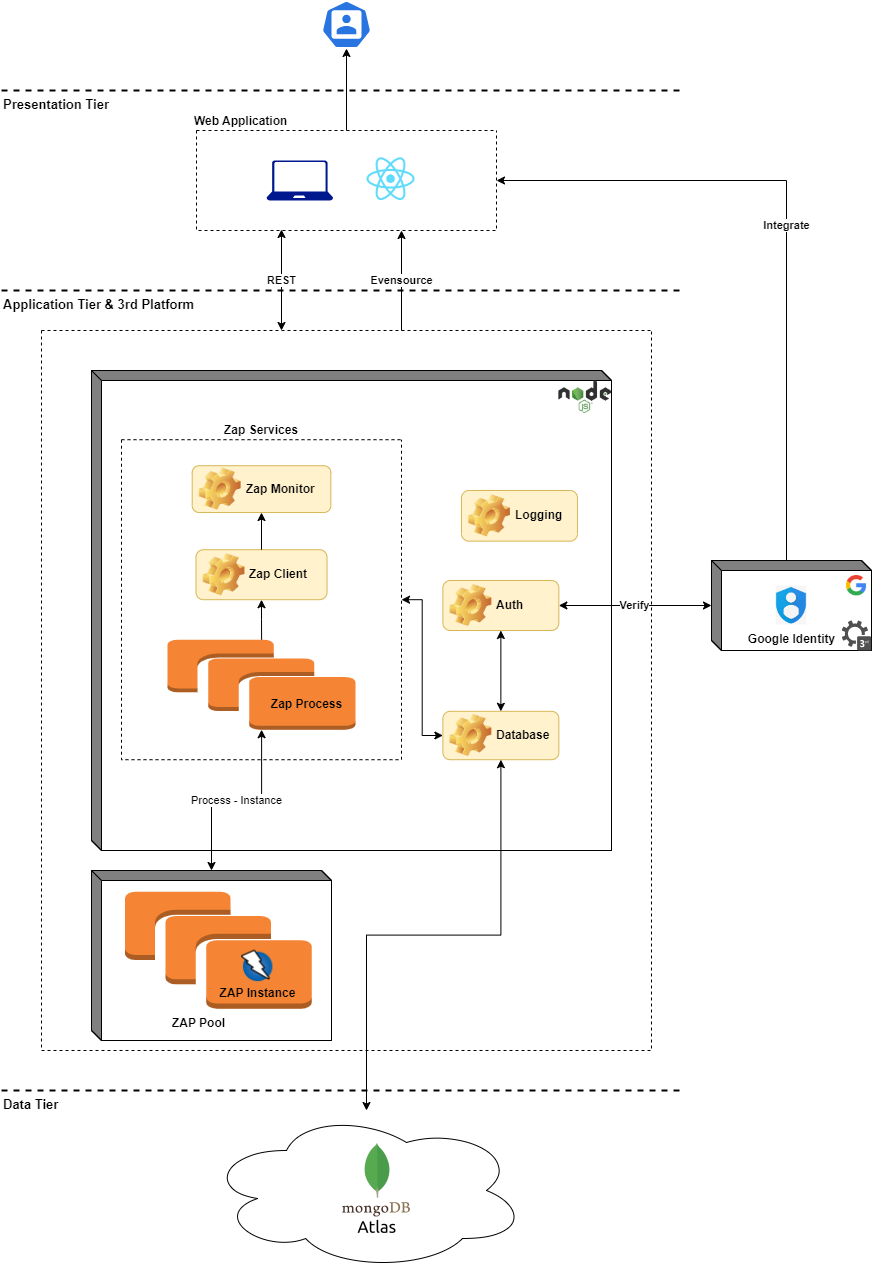
\includegraphics[width=\textwidth]{applied-thesis-chapters/chapter-3/Tổng quan kiến trúc hệ thống.png}
      \caption{Tổng quan kiến trúc hệ thống}
      \label{fig:KienTrucHeThong}
\end{figure}

Hình \textit{\ref{fig:KienTrucHeThong} \nameref{fig:KienTrucHeThong}} thể hiện tổng quan kiến trúc hệ thống được xây dựng theo mô hình N-Tier đã đề cập ở mục \textit{\ref{sec:NTier} \nameref{sec:NTier}}.
Kiến trúc hệ thống gồm 3 tầng (3-Tier): Tầng trình bày, tầng ứng dụng và tầng dữ liệu.

\subsubsection{Thiết kế kiến trúc hệ thống tầng trình bày}

\tab Tầng trình bày (Presentation tier) là tầng dành cho ứng dụng web, phục vụ cho người dùng.
Người dùng tương tác trên giao diện ứng dụng web để tiếp cận với các giải pháp mà nhóm đã đề cập đến ở mục \textit{\ref{sec:AbstractSol} \nameref{sec:AbstractSol}}.
Theo như kiến trúc, ứng dụng web của tầng trình bày được xây dựng chính bằng thư viện React và các công cụ có hỗ trợ React.

\subsubsection{Thiết kế kiến trúc hệ thống tầng ứng dụng} \label{subsubsec:ThietKeKienTrucTangUngDung}

\tab Tầng ứng dụng (Application tier) là tầng có trách nhiệm xử lý đa phần mọi giải pháp của hệ thống, là tầng chính của toàn bộ hệ thống.
Theo như kiến trúc, tầng ứng dụng chứa 2 phần là ứng dụng chính và tập hợp các đối tượng ZAP (ZAP Pool).
Ứng dụng của tầng này được xây dựng với framework Express.js trên nền tảng Node.js.

Ứng dụng chính bao gồm các dịch vụ (service) được cài đặt tách biệt với nhau, mang nhiệm vụ riêng để tăng tính trực quan và linh hoạt, khả năng mở rộng và bảo trì, tránh các lỗi xung đột không đáng có, dễ dàng phát triển và tích hợp.
Các service bao gồm: Nhóm các ZAP service, Dịch vụ xác thực (Authentication service), Dịch vụ cơ sở dữ liệu (Database service) và Dịch vụ ghi nhật ký (Logging service).
\par

\myparagraph{Nhóm ZAP service}
\tab \tab Nhóm các ZAP service bao gồm 2 service chính là dịch vụ quản lý ZAP (ZAP Monitor service) và dịch vụ tương tác với ứng dụng ZAP (ZAP Client service), cuối cùng là lớp tiến trình ZAP (ZAP Process).
Hình \textit{\ref{fig:NhomZapServiceHoatDong} \nameref{fig:NhomZapServiceHoatDong}} sẽ cho ta cái nhìn chi tiết hơn về cách hoạt động của nhóm ZAP service trong hệ thống.

\begin{figure}[H]
      \centering
      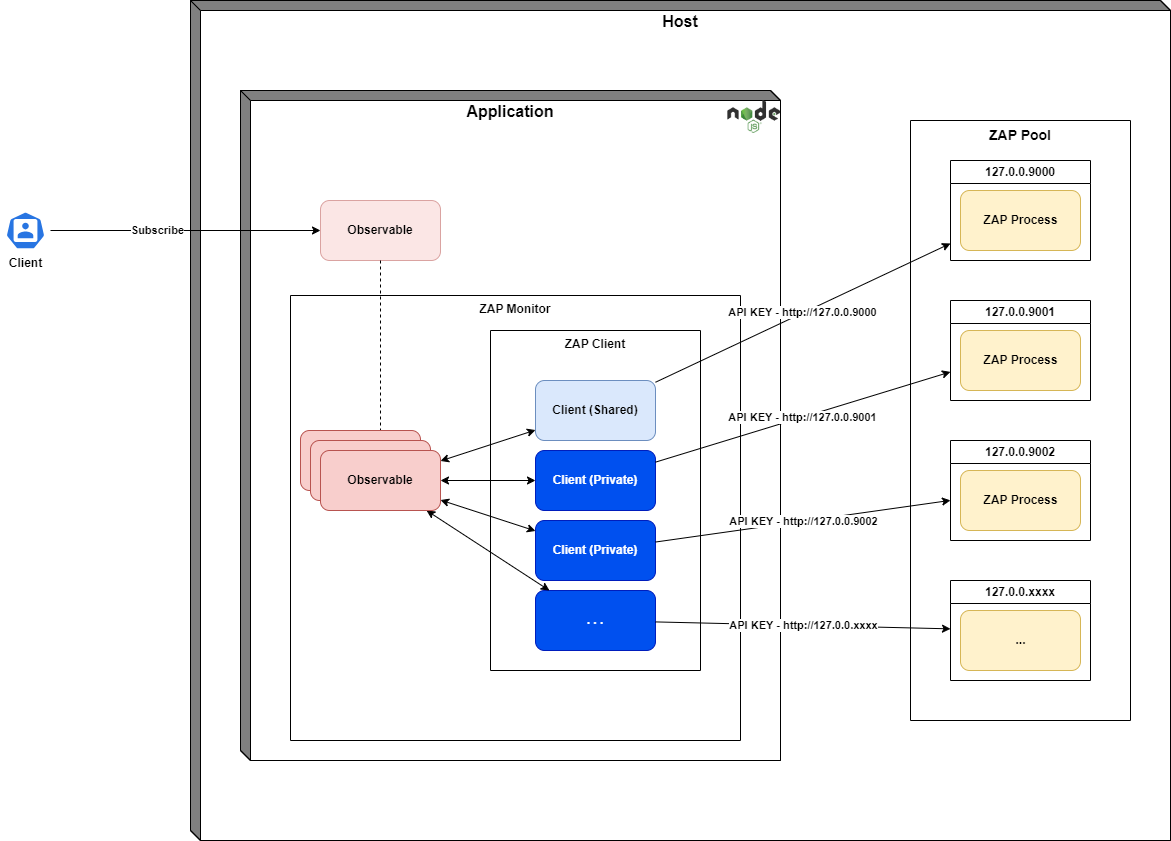
\includegraphics[width=\textwidth]{applied-thesis-chapters/chapter-3/Mô tả nhóm ZAP service hoạt động trong hệ thống.png}
      \caption{Mô tả nhóm ZAP service hoạt động trong hệ thống}
      \label{fig:NhomZapServiceHoatDong}
\end{figure}

\begin{itemize}
      \item \textbf{ZAP Process:} Mỗi tiến trình ZAP sẽ được khởi tạo từ lớp ZAP Process, gọi là ZAP Process instance.
            Mỗi instance là process chạy ngầm trong hệ thống (trình nền, hay còn gọi là daemon).
            Các instance này hoạt động lập với nhau trên các cổng (port) khác nhau như một ứng dụng được khởi chạy riêng biệt.
      \item \textbf{ZAP Client service:} Service có nhiệm vụ tạo và quản lý các ZAP client.
            Mỗi ZAP client được service quản lý qua một mã định danh duy nhất (UUID - Universally Unique Identifier) và tham chiếu đến mỗi ZAP Process instance khác nhau.
            ZAP client có vai trò tương tác, điều khiển ZAP process thực hiện các tác vụ của ZAP qua phương thức HTTP.
            Vì ZAP process chỉ là một process chạy ngầm trong hệ thống và tách biệt với ứng dụng chính nên ZAP Client service là một trong những service quan trọng của ứng dụng chính.
            Theo như giải pháp thì mỗi phương pháp quét sẽ cần mỗi ZAP process có hành vi, cấu hình khác nhau.
            Nhóm chia thành 2 loại là:
            \begin{itemize}
                  \item \textbf{ZAP Client Shared:} Client này dành cho các phương pháp quét có thể sử dụng chung ZAP process instance, kết quả các phiên quét tuy sử dụng chung instance nhưng không ảnh hưởng đến nhau.
                        Cặp client shared và ZAP process và luôn luôn tồn tại xuyên suốt quá trình sống của ứng dụng.
                  \item \textbf{ZAP Client Private:} Client này dành cho các phương pháp quét không thể sử dụng chung ZAP process instance.
            \end{itemize}
      \item \textbf{ZAP Monitor service:} Service có vai trò đại diện cho nhóm ZAP service.
            Cài đặt của các giải pháp của ứng dụng chính chỉ giao tiếp với service này.
            Service có nhiệm vụ tạo, dừng và quản lý các phiên quét của người dùng; nắm giữ và quản lý quá trình quét của các phiên quét, giúp cho hệ thống có thể kết nối và biết được các thông tin về trạng thái và tiến độ của phiên quét; lưu trữ các dữ liệu cần thiết khi hoạt động với ZAP như thông tin phiên quét, thông tin kết quả với Database service.
\end{itemize}

\newpage
\myparagraph{ZAP Pool}
\tab \tab Là tập hợp các ZAP process instance chạy ngầm, mỗi instance sẽ chạy trên một cổng (port) khác nhau và được tham chiếu bởi các ZAP client của ZAP Client service.
\par

Các hình \textit{\ref{fig:TTZapMonitorStartScan} \nameref{fig:TTZapMonitorStartScan}} và \textit{\ref{fig:TTHeThongStartScan} \nameref{fig:TTHeThongStartScan}} thể hiện quá trình tương tác và hoạt động của nhóm ZAP service trong hệ thống khi bắt đầu một phiên quét.

\begin{figure}[H]
      \centering
      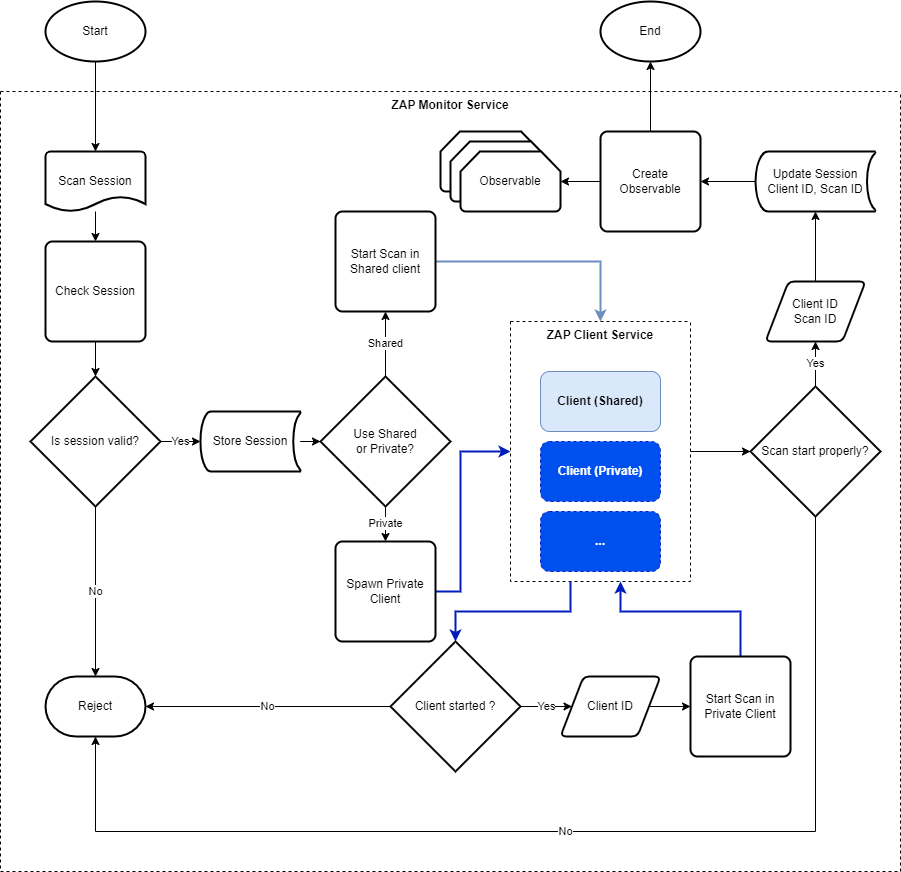
\includegraphics[width=\textwidth]{applied-thesis-chapters/chapter-3/Sơ đồ tuần tự của quá trình bắt đầu phiên quét của ZAP Monitor service.png}
      \caption{Sơ đồ tuần tự của quá trình bắt đầu phiên quét của ZAP Monitor service}
      \label{fig:TTZapMonitorStartScan}
\end{figure}

\begin{figure}[H]
      \centering
      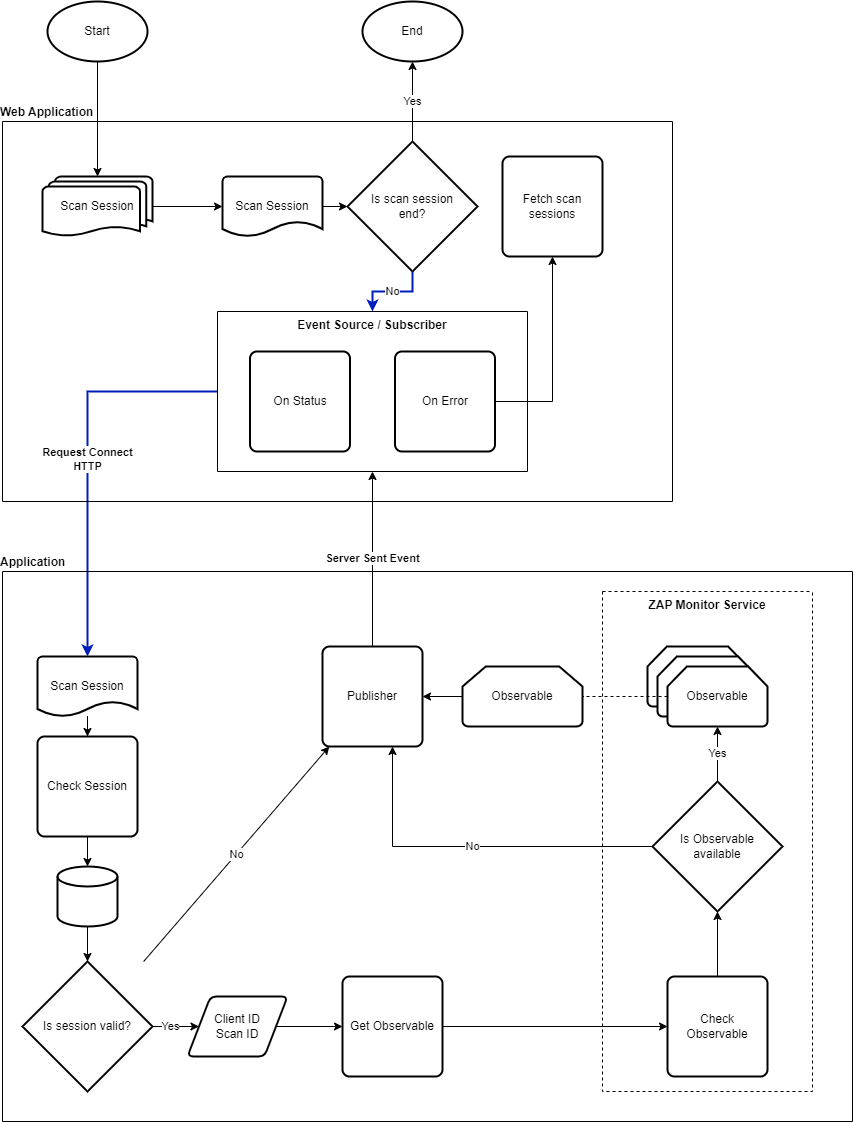
\includegraphics[width=\textwidth]{applied-thesis-chapters/chapter-3/Sơ đồ tuần tự của quá trình bắt đầu phiên quét của hệ thống với ứng dụng web.png}
      \caption{Sơ đồ tuần tự của quá trình bắt đầu phiên quét của hệ thống với ứng dụng web}
      \label{fig:TTHeThongStartScan}
\end{figure}

\myparagraph{Authentication service}
\tab \tab Service thực hiện các nhiệm vụ liên quan đến xác thực người dùng.
Các nhiệm vụ như xác minh lại token nhận được từ ứng dụng web từ bên thứ ba là Google Identify, đọc ghi dữ liệu người dùng với Database service.

\myparagraph{Logging service}
\tab \tab Service có trách nhiệm ghi lại nhật ký (log) cho toàn bộ ứng dụng, bao gồm cả các ZAP process chạy ngầm.
Service được cài đặt.vì các ZAP process được chạy ngầm nằm ngoài phạm vi của ứng dụng, và nhu cầu lấy log của các process này là cần thiết.
Log của các service khác nhau được phân biệt bằng tên loại khác nhau, các tên này được sử dụng làm tiền tố của mỗi dòng log khi hiển thị trong bảng điều khiển (console).
Chủ yếu có 4 loại log hiện có trong ứng dụng là:

\begin{itemize}
      \item \textbf{Main process log:} Các log này trình bày các tác vụ, lỗi phát sinh bên trong ứng dụng chính, đa phần nằm trong ZAP Monitor service.
      \item \textbf{Http request log:} Các log này trình bày thông tin chi tiết các yêu cầu (request) được gửi đến ứng dụng ở mọi tuyến (route).
      \item \textbf{User session process log:} Các log này trình bày thông tin các kết nối của người dùng với các phiên quét.
            Mỗi phiên quét sẽ có quá trình quét, các quá trình quét sẽ được quản lý bởi ZAP Monitor service, thông tin của phiên quét là trạng thái và tiến độ sẽ được gửi đến người dùng theo thời gian thực (stream).
            Thông tin các kết nối stream của người dùng sẽ được ghi lại trong loại log này.
      \item \textbf{ZAP process log:} Log này được nhúng vào mỗi ZAP process khi chúng vừa được khởi tạo.
            Nội dung của các log này giống với log của chính trình nền đang chạy ZAP process đó.
            Hiển thị theo thời gian thực giống với trình nền đó.
            Theo như nghiệp vụ của giải pháp, loại log này còn có một biến thể nữa là ZAP private process log.
            ZAP process log bình thường sẽ ghi lại các log trong ZAP shared process instance, còn ZAP private process log sẽ ghi lại các log trong các ZAP private process instance.
\end{itemize}

\myparagraph{Database service}
\tab \tab Service có nhiệm vụ là kết nối với MongoDB Atlas và đại diện thực hiện các thao tác đọc ghi, truy vấn với cơ sở dữ liệu đã kết nối.

\subsubsection{Thiết kế kiến trúc hệ thống tầng dữ liệu}

\tab Tầng dữ liệu là tầng cơ sở dữ liệu, nơi các dữ liệu của hệ thống được lưu trữ.
Các dữ liệu được lưu trữ trong hệ thống là thông tin định danh người dùng, các dữ liệu liên quan đến mục tiêu và phiên quét.
\par

Cơ sở dữ liệu MongoDB là một cơ sở dữ liệu hướng tài liệu, thuộc dạng cơ sở dữ liệu phi quan hệ (NoSQL).
Bản ghi dữ liệu trong MongoDB được ghi đệm (cache) lên RAM (Random Access Memory) khi có truy vấn đến nó, hạn chế truy cập vào ổ cứng nên tốc độ đọc ghi cao.
\par

Nhóm đề xuất sử dụng MongoDB làm cơ sở dữ liệu do các tính chất trên phù hợp với giải pháp ứng dụng.
Giải pháp ứng dụng yêu cầu ghi nhiều loại dữ liệu có cấu trúc linh hoạt, đa dạng.
Các dữ liệu có cấu trúc linh hoạt tiêu biểu như:

\begin{itemize}
      \item Bản ghi cấu hình và kết quả của phiên quét của các phương thức quét khác nhau.
      \item Bản ghi thông tin phiên quét trong quá trình quét cần đọc ghi nhiều lần.
\end{itemize}

Tiếp theo, như đã nhắc đến ở trên, bản ghi dữ liệu của MongoDB có thể cache lên RAM để tăng tốc truy vấn dữ liệu và mặc định sử dụng 50% RAM trên hệ thống.
Cùng với việc hệ thống thường phải hoạt động với cường độ cao, sử dụng 80 đến 90% hiệu suất Bộ xử lý trung tâm (Central Processing Unit, viết tắt là CPU) và 60 đến 70% hiệu suất RAM, khi thực hiện nhiều phiên quét cùng lúc. 
Vậy nên rủi ro dữ liệu không được ghi một cách đúng đắn khi hệ thống hoạt động hiệu suất cao là có tồn tại.
\par

Để giải quyết vấn đề này, nhóm đề xuất sử dụng MongoDB Atlas là một dịch vụ cơ sở dữ liệu đám mây (cloud database service).
MongoDB Atlas là một cloud database dành riêng và thuộc sự quản lý trực tiếp của MongoDB.
Về bản chất, database được triển khai hoàn toàn trên VPC là Google Cloud Platform, AWS hay Microsoft Azure dựa theo tùy chọn khi khởi tạo.
Người dùng có thể kết nối, quản lý, tương tác qua trung gian MongoDB Atlas.
Như hình \textit{\ref{fig:KetNoiAtlas} \nameref{fig:KetNoiAtlas}}, ứng dụng chính tương tác với database trên VPC bằng trình điều khiển MongoDB (MongoDB driver) qua phương thức TCP/IP socket.
\par

\begin{figure}[H]
      \centering
      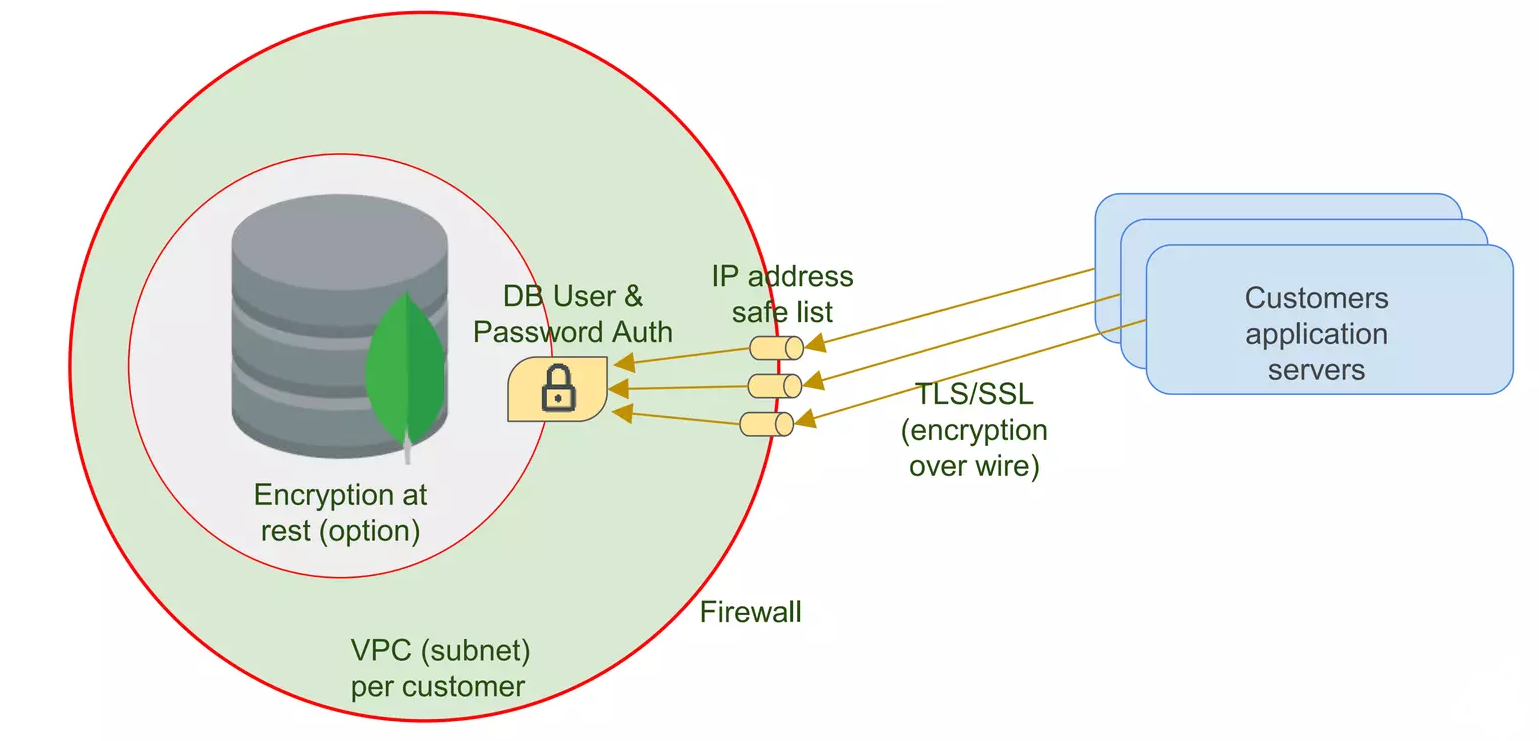
\includegraphics[width=\textwidth]{applied-thesis-chapters/chapter-3/Mô tả kết nối của ứng dụng với MongoDB Atlas.png}
      \caption{Mô tả kết nối của ứng dụng với MongoDB Atlas}
      \label{fig:KetNoiAtlas}
\end{figure}

Về cơ bản, nhóm triển khai MongoDB trên một máy dịch vụ khác, không triển khai chung với hệ thống để tránh các vấn đề hiệu suất hệ thống ảnh hưởng đến toàn vẹn dữ liệu.
Chuyển sự hạn chế bởi cấu hình của MongoDB sang máy khác nghĩa là không còn giữ nguyên được tính nhanh chóng (cache) và các tương tác với database phải thông qua giao thức TCP/IP socket (chức năng cache vẫn hoạt động bình thường ở VPC).
Bên cạnh lợi ích toàn vẹn dữ liệu, việc lựa chọn giải pháp này cũng mang lại nhiều lợi ích khác như tăng tính bảo mật, mở rộng, linh hoạt, tiện lợi, dễ dàng quản lý và không cần nhiều bận tâm về các vấn đề của database trên hệ thống chính.

\newpage
\subsection{Thiết kế giao diện ứng dụng web}

\subsubsection{Thiết kế màn hình trang chủ}

\tab Màn hình trang chủ là nơi người dùng sẽ tiếp cận đầu tiên khi truy cập vào tên miền gốc của ứng dụng.
Màn hình có 2 thành phần chính là giới thiệu chung về ứng dụng và phần cho phép người dùng sử dụng thử chức năng quét với phương thức ZAP Spider, không cần đăng nhập xác minh.
Màn hình trang chủ được thiết kế như hình \textit{\ref{fig:MHTrangChu} \nameref{fig:MHTrangChu}}.

\begin{figure}[H]
      \centering
      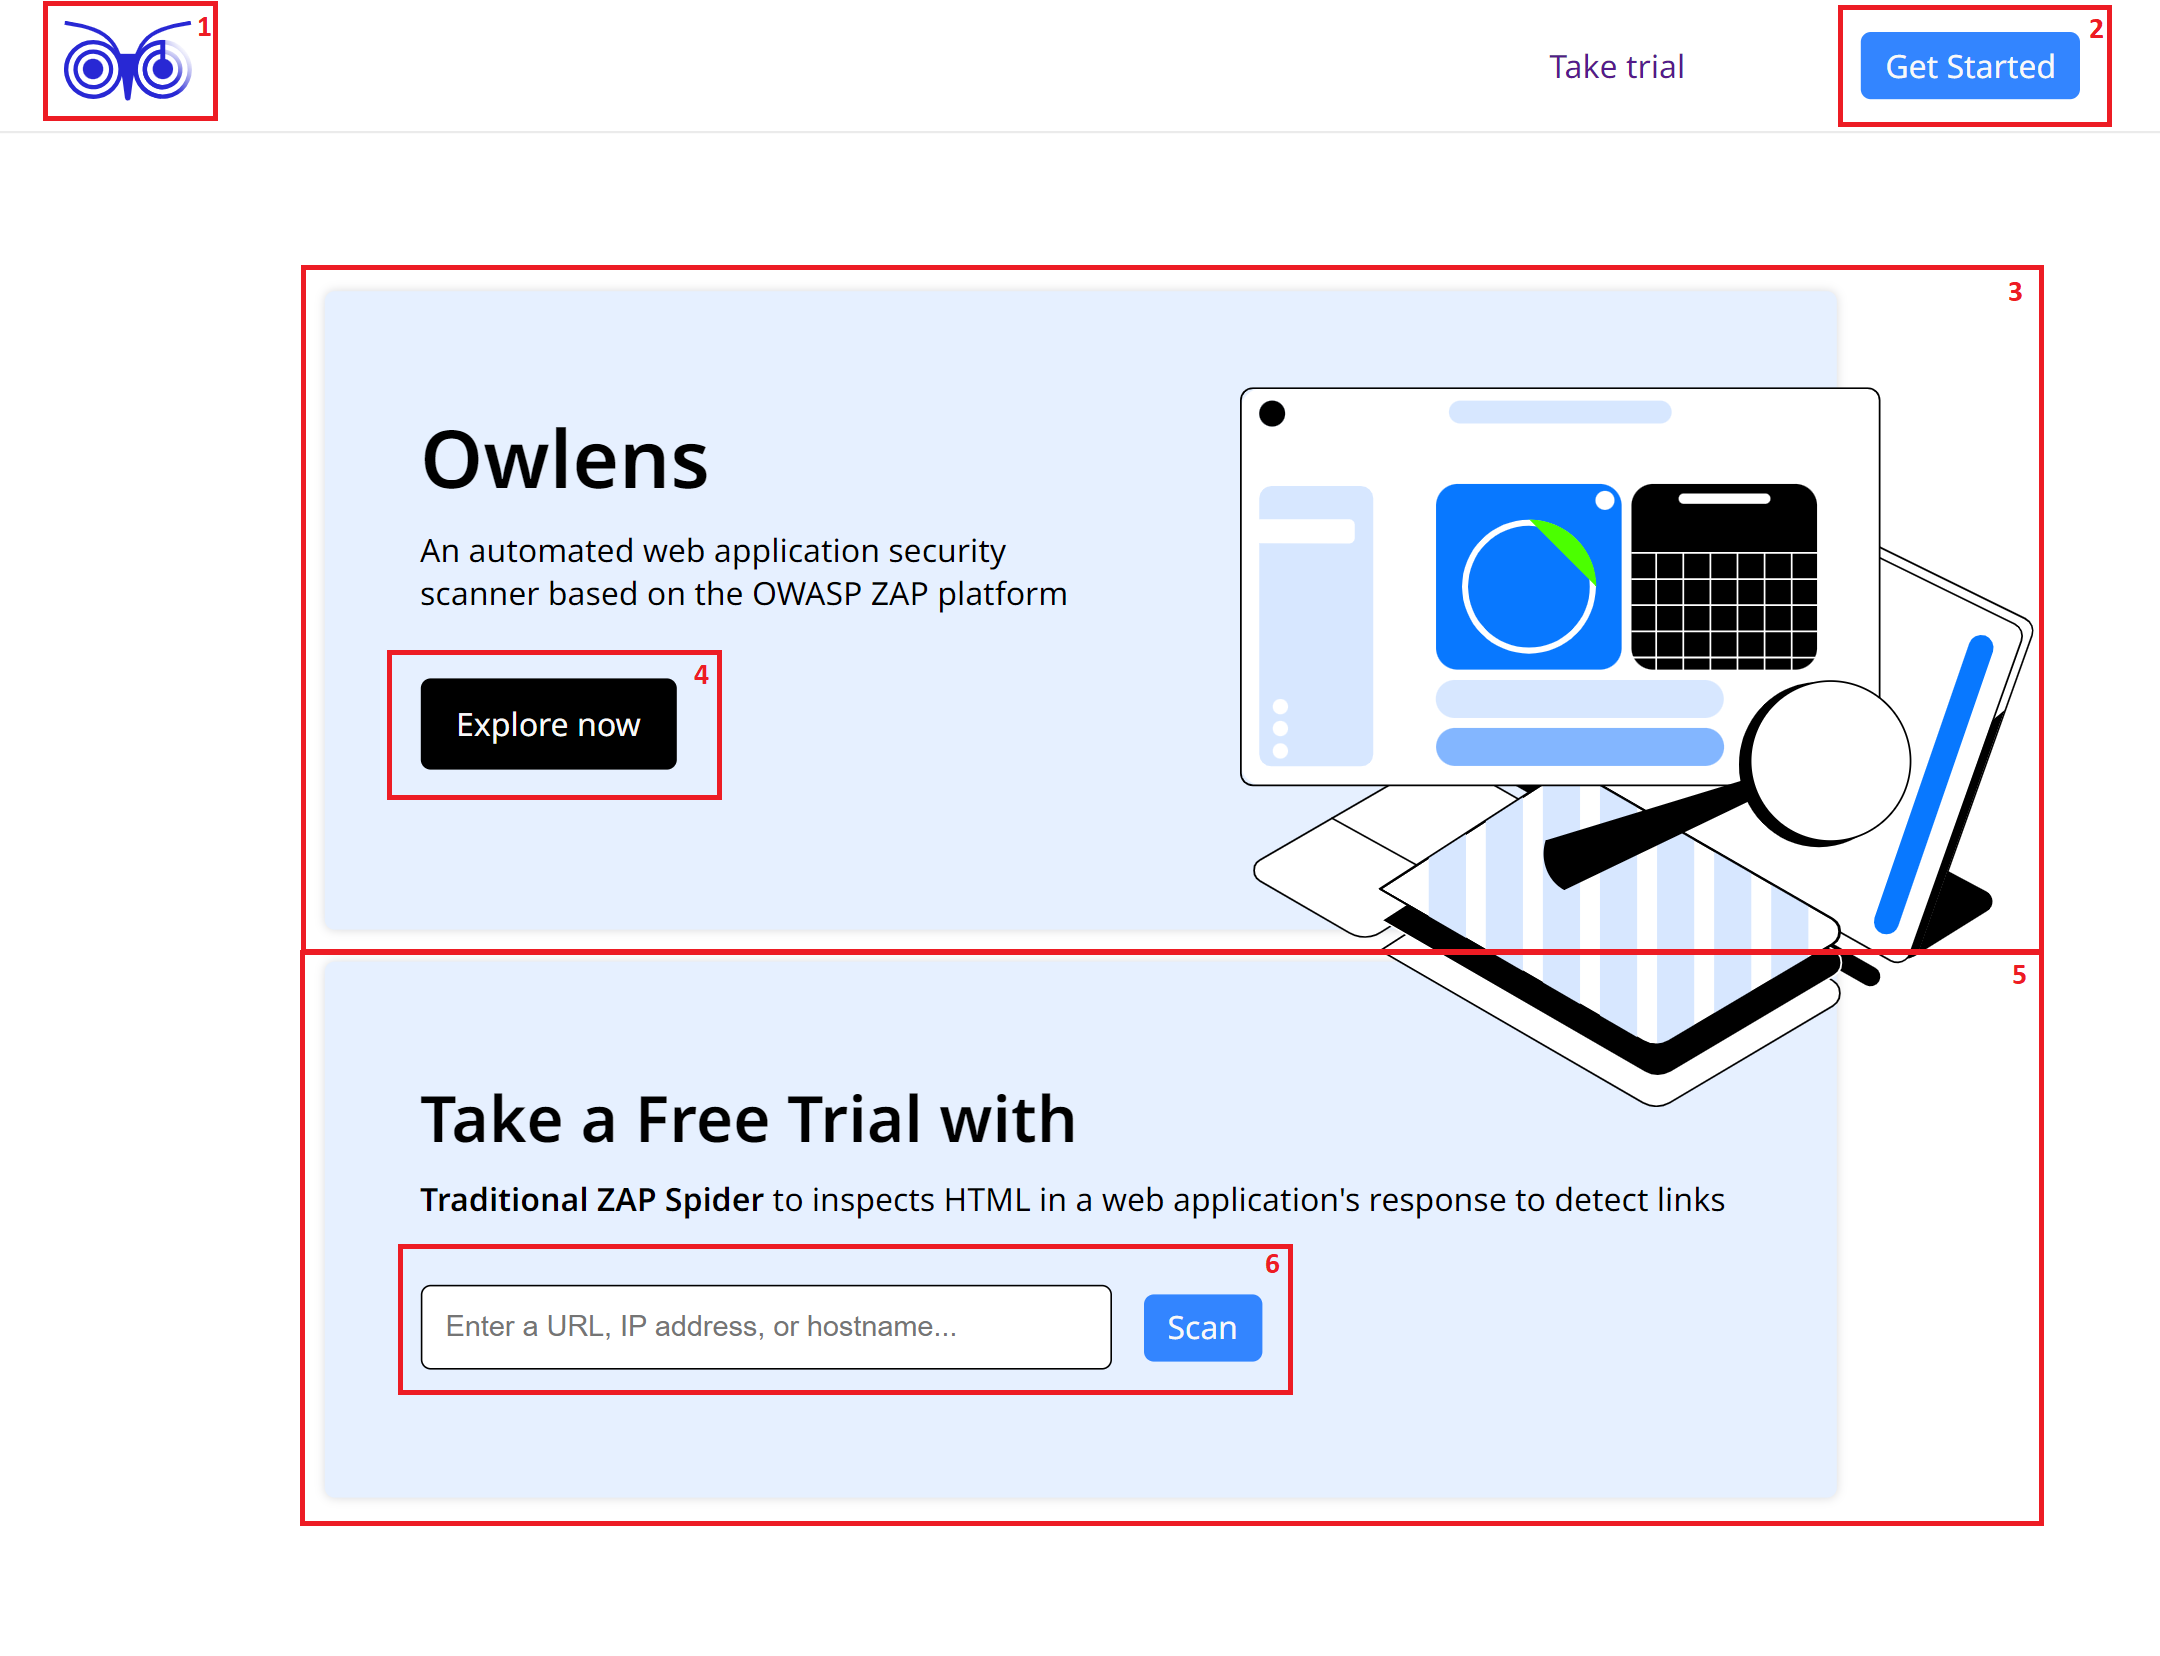
\includegraphics[width=\textwidth]{applied-thesis-chapters/chapter-3/Màn hình trang chủ.png}
      \caption{Màn hình trang chủ}
      \label{fig:MHTrangChu}
\end{figure}

\newpage
Mô tả giao diện màn hình trang chủ được thể hiện qua bảng \textit{\ref{tab:MTTrangChu} \nameref{tab:MTTrangChu}}:

\begin{tabularx}{\textwidth}{|>{\hsize=.10\hsize\centering\let\newline
      \\\arraybackslash}X|>{\hsize=.30\hsize\raggedright\let\newline
      \\\arraybackslash}X|>{\hsize=.50\hsize\raggedright\let\newline
      \\\arraybackslash}X|}
      \hline
      \thead{STT}
       & \thead{Tên thành phần}
       & \thead{Mô tả}
      \\
      \hline
      1
       &
      Logo
       &
      Logo của ứng dụng Owlens. Có thể chọn vào logo để điều hướng quay lại màn hình trang chủ.
      \\
      \hline
      2
       &
      Nút bắt đầu
       &
      Dùng để điều hướng đến trang đăng nhập và đăng ký của hệ thống.
      \\
      \hline
      3
       &
      Phần giới thiệu
       &
      Phần này giới thiệu thông tin, chức năng chung của hệ thống.
      \\
      \hline
      4
       &
      Nút gọi hành động (Call to Action, viết tắt là CTA)
       &
      Dùng để điều hướng đến trang đăng nhập và đăng ký của hệ thống.
      \\
      \hline
      5
       &
      Phần giới thiệu dùng thử
       &
      Giới thiệu thông tin phần dùng thử. Người dùng có thể sử dụng thử chức năng quét với phương thức ZAP Spider mà không cần đăng nhập xác minh.
      \\
      \hline
      6
       &
      Phần dùng thử
       &
      Người dùng dùng thử bằng cách nhập URL hoặc IP và chọn nút “Scan“ để bắt đầu phiên quét. Kết quả quét sẽ được hiển thị trực tiếp theo thời gian thực ngay trên cùng màn hình trang chủ, trong phần dùng thử. Vì không cần xác minh nên đối với kết quả quét xong, kết quả sẽ biến mất khi người dùng di chuyển ra khỏi màn hình trang chủ. Đối với kết quả đang được hiển thị trực tiếp, đang trong quá trình quét thì kết quả sẽ biến mất khi người dùng di chuyển quá 60 giây khỏi màn hình trang chủ.
      \\
      \hline
      \caption{Mô tả giao diện màn hình trang chủ}
      \label{tab:MTTrangChu}
\end{tabularx}

\newpage
\subsubsection{Màn hình ứng dụng}

\tab Màn hình ứng dụng là nơi người dùng sẽ tiếp cận sau khi đăng nhập vào ứng dụng.
Màn hình này là nơi người dùng thực hiện hầu hết mọi tác vụ có trong ứng dụng.
Màn hình có 2 thành phần chính là bảng tùy chọn và bản điều khiển.
Màn hình ứng dụng được thiết kế như hình \textit{\ref{fig:MHUngDung} \nameref{fig:MHUngDung}}.

\begin{figure}[H]
      \centering
      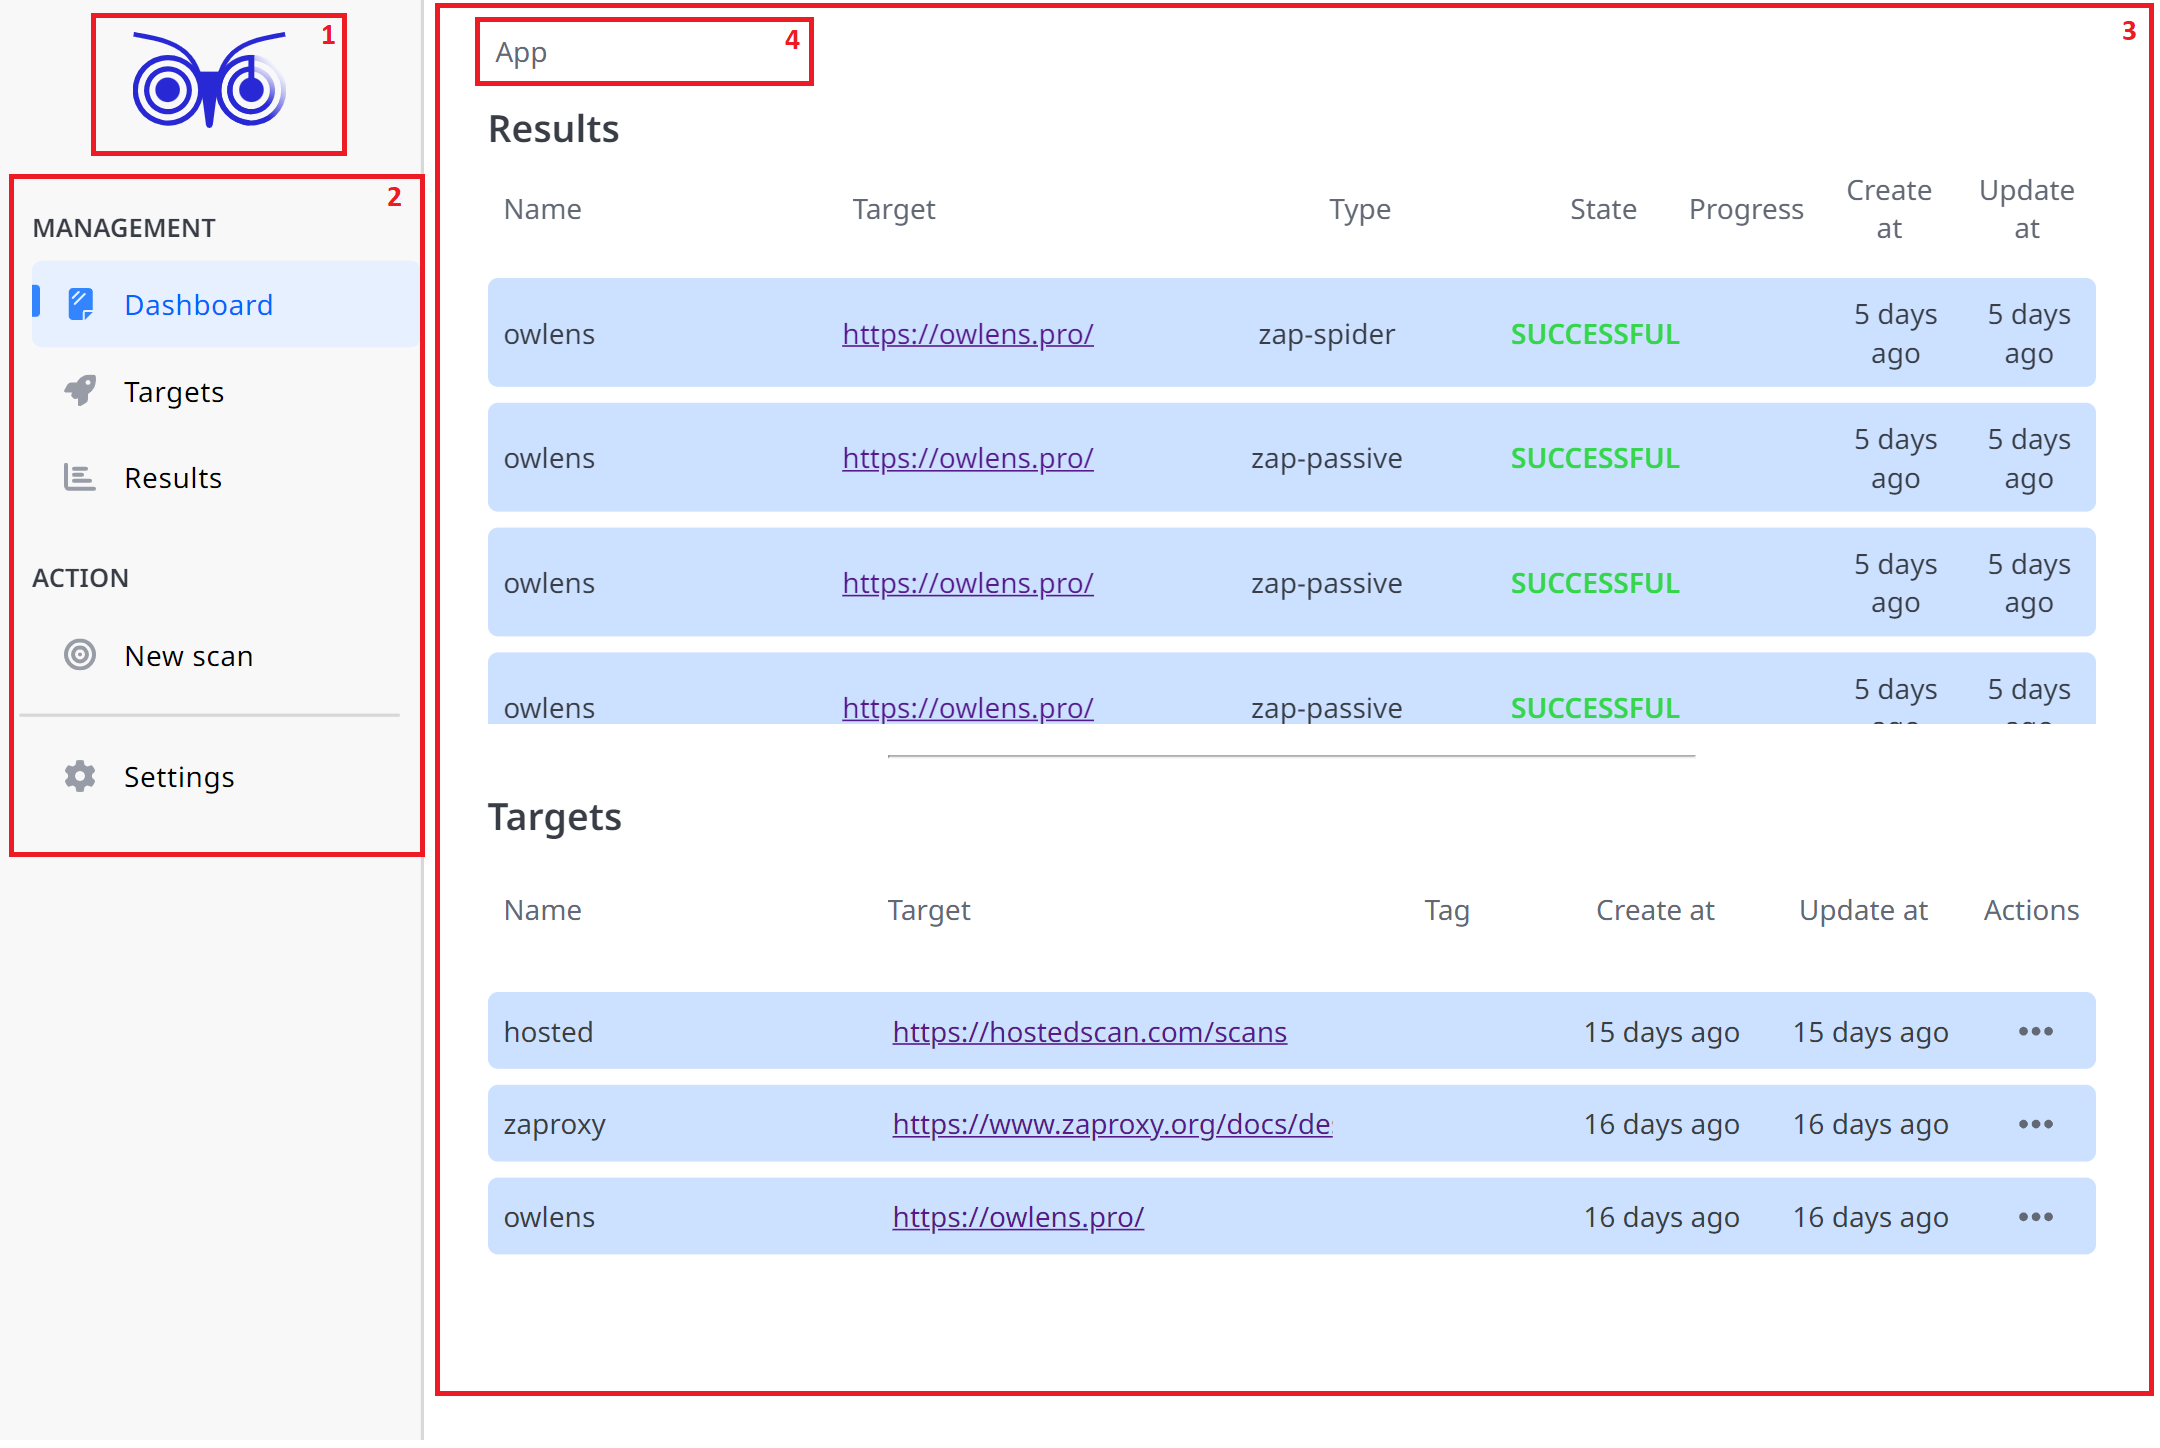
\includegraphics[width=\textwidth]{applied-thesis-chapters/chapter-3/Màn hình ứng dụng.png}
      \caption{Màn hình ứng dụng}
      \label{fig:MHUngDung}
\end{figure}

Mô tả giao diện màn hình ứng dụng được thể hiện qua bảng \textit{\ref{tab:MTUngDung} \nameref{tab:MTUngDung}}:

\begin{tabularx}{\textwidth}{|>{\hsize=.10\hsize\centering\let\newline
      \\\arraybackslash}X|>{\hsize=.30\hsize\raggedright\let\newline
      \\\arraybackslash}X|>{\hsize=.50\hsize\raggedright\let\newline
      \\\arraybackslash}X|}
      \hline
      \thead{STT}
       & \thead{Tên thành phần}
       & \thead{Mô tả}
      \\
      \hline
      1
       &
      Logo
       &
      Logo của ứng dụng Owlens. Người dùng có thể chọn vào logo để quay lại màn hình chính của ứng dụng cũng là màn hình của tùy chọn “Dashboard“.
      \\
      \hline
      2
       &
      Bảng tùy chọn
       &
      Người dùng có thể chuyển đổi giữa các bảng điều khiển bằng khác nhau tương ứng với các tùy chọn có trong bảng tùy chọn.
      \\
      \hline
      3
       &
      Bảng điều khiển
       &
      Bảng hiển thị các nội dung khác nhau tương ứng với các tùy chọn đang được chọn khác nhau.
      \\
      \hline
      4
       &
      Thanh truy vết địa chỉ
       &
      Cho phép người dùng theo dõi vị trí hiện tại trong ứng dụng và di chuyển lại truy vết trước đó.
      \\
      \hline
      \caption{Mô tả giao diện màn hình ứng dụng}
      \label{tab:MTUngDung}
\end{tabularx}

\section{Sơ đồ phần mềm hệ thống}

\subsection{Sơ đồ use case}

\tab Sơ đồ Use Case của hệ thống được thể hiện qua hình \textit{\ref{fig:UseCase} \nameref{fig:UseCase}}.

\begin{figure}[H]
      \centering
      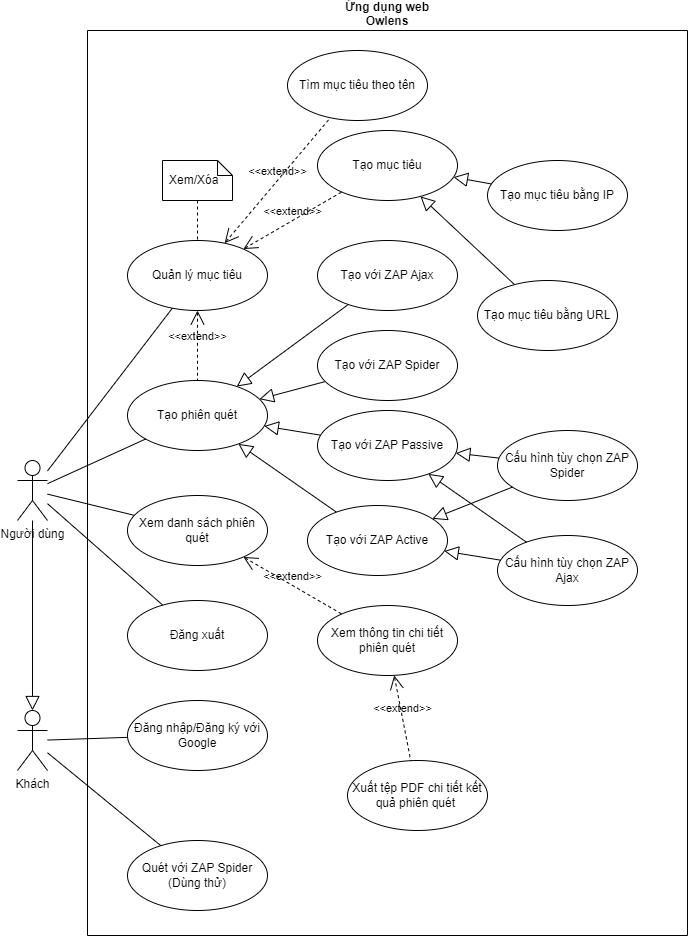
\includegraphics[width=\textwidth]{applied-thesis-chapters/chapter-3/Sơ đồ Use Case.png}
      \caption{Sơ đồ Use Case}
      \label{fig:UseCase}
\end{figure}

Sơ đồ Use Case của hệ thống được mô tả qua bảng \textit{\ref{tab:UseCase} \nameref{tab:UseCase}}.

\begin{tabularx}{\textwidth}{|>{\hsize=.10\hsize\centering\let\newline
      \\\arraybackslash}X|>{\hsize=.30\hsize\raggedright\let\newline
      \\\arraybackslash}X|>{\hsize=.50\hsize\raggedright\let\newline
      \\\arraybackslash}X|}
      \hline
      \thead{STT}
       & \thead{Use Case}
       & \thead{Mô tả}
      \\
      \hline
      1
       &
      Đăng nhập/Đăng ký với Google
       &
      Người dùng khách có thể đăng nhập vào hệ thống bằng tài khoản Google, nếu tài khoản của người dùng đăng nhập lần đầu sẽ được ghi nhận như đăng ký và đăng nhập cùng lúc.
      \\
      \hline
      2
       &
      Quét với ZAP Spider (Dùng thử)
       &
      Người dùng khách có thể sử dụng thử chức năng quét với ZAP Spider. Vì là khách nên kết quả quét chỉ được hiển thị chứ không lưu vào hệ thống.
      \\
      \hline
      3
       &
      Quản lý mục tiêu
       &
      Người dùng đã đăng nhập có thể xem danh sách mục tiêu, tạo và xóa các mục tiêu. Khi xem danh sách mục tiêu người dùng có tìm mục tiêu theo tên. Khi tạo mục tiêu, người dùng có thể tạo 2 loại mục tiêu: mục tiêu bằng URL và mục tiêu bằng IP.
      \\
      \hline
      4
       &
      Tạo phiên quét
       &
      Người dùng đã đăng nhập có thể tạo phiên quét mới từ các mục tiêu đã tạo. Các phương thức của phiên quét người dùng có thể chọn là: ZAP Spider, ZAP Ajax, ZAP Passive, ZAP Active. Ngoài ra, khi tạo các phiên quét bằng ZAP Passive hay ZAP Active, người dùng có thể chọn cấu hình loại khám phá (explore type) là ZAP Spider hoặc ZAP Ajax (mặc định là ZAP Spider).
      \\
      \hline
      5
       &
      Xem danh sách phiên quét
       &
      Người dùng đã đăng nhập có thể xem danh sách phiên quét. Danh sách phiên quét hiển thị thông tin chung của các phiên quét. Người dùng có thể chọn mục trong bảng để xem thông tin chi tiết của phiên quét. Trong màn hình của thông tin chi tiết phiên quét, người dùng có thể chọn xuất kết quả quét ra tệp PDF.
      \\
      \hline
      6
       &
      Đăng xuất
       &
      Người dùng đã đăng nhập có thể đăng xuất phiên đăng nhập của mình khỏi hệ thống.
      \\
      \hline
      \caption{Mô tả sơ đồ Use Case}
      \label{tab:UseCase}
\end{tabularx}

\newpage
\subsection{Sơ đồ cơ sở dữ liệu}

Sơ đồ cơ sở dữ liệu của hệ thống được thể hiện qua hình \textit{\ref{fig:Database} \nameref{fig:Database}}.

\begin{figure}[H]
      \centering
      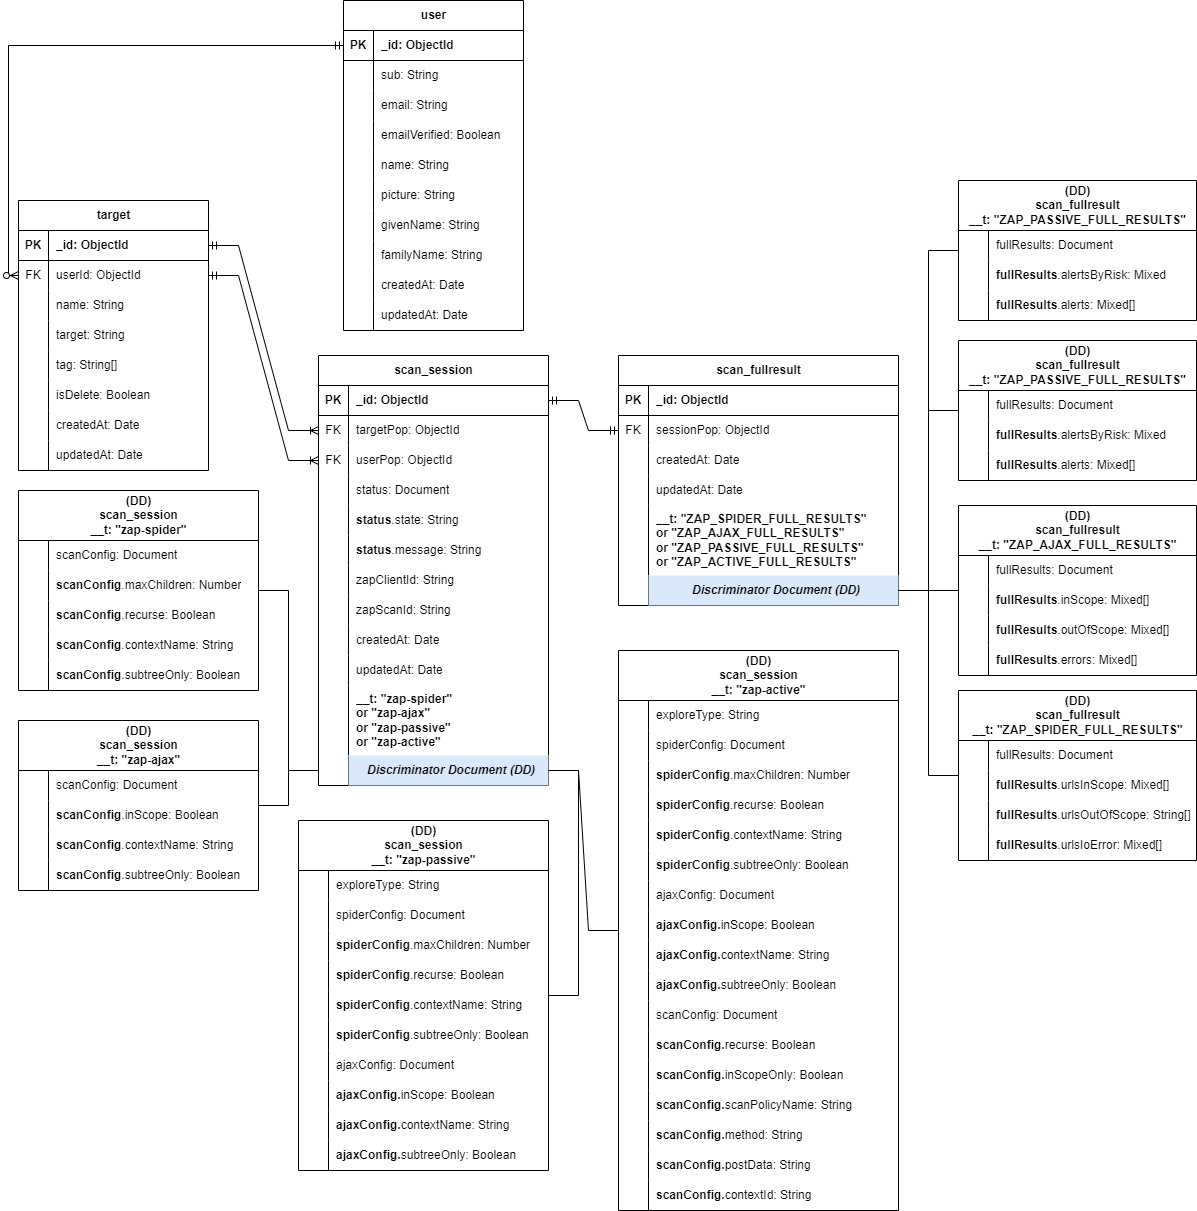
\includegraphics[width=\textwidth]{applied-thesis-chapters/chapter-3/Sơ đồ cơ sở dữ liệu.png}
      \caption{Sơ đồ cơ sở dữ liệu}
      \label{fig:Database}
\end{figure}
\chapter{CÀI ĐẶT GIẢI PHÁP}

\section{RKT Query}

\tab Nhóm sử dụng thư viện React, là một thư viện JavaScript giúp xây dựng giao diện người dùng, để phát triển ứng dụng web.
Khi sử dụng React thì việc quản lý trạng thái ứng dụng (state) là một trong những vấn đề tiên quyết cần giải quyết.
Nhóm chọn sử dụng thư viện Redux để giải quyết vấn đề này.
Redux là một thư viện JavaScript, dùng để quản lý state ứng dụng, được sử dụng rộng rãi trong hệ sinh thái React.
\par

Trong quá khứ, trước phiên bản React 16.8, để có thể theo dõi trạng thái và vòng đời của một thành phần React (React component) thì sử dụng thành phần lớp React (React class component) là cách duy nhất.
Khi đó, việc sử dụng Redux trong ứng dụng React có đôi chút khó khăn và dài dòng do cú pháp, cấu trúc phức tạp.
Từ phiên bản React 16.8, với sự xuất hiện của thành phần hàm React (React functional component) là cách khởi tạo React component mới, cùng với sự xuất hiện của React Hook là cách quản lý trạng thái và vòng đời của component trong React functional component, thì Redux cũng được cải tiến để phù hợp với sự thay đổi này đó là sự xuất hiện của thư viện Redux Tookit.
Do đó, đề xuất sử dụng Redux của nhóm chính là sử dụng Redux Tookit.
\par

\textit{"Redux Toolkit là phương pháp tiêu chuẩn chính thức để viết logic Redux.
Nó bao bọc xung quanh lõi của Redux, và chứa các gói và hàm được cho là cần thiết để xây dựng một ứng dụng Redux.
Redux Toolkit tích hợp các thực hành tốt nhất (best practices) được đề xuất, đơn giản hóa hầu hết các tác vụ Redux, ngăn ngừa những sai lầm phổ biến và làm cho việc viết ứng dụng Redux dễ dàng hơn."} \cite{chap4bib1}
\par

Trong phạm vi khóa luận, khi xây dựng ứng dụng web thì việc tương tác và quản lý dữ liệu API cũng là một vấn đề tiên quyết.
Khi muốn đưa dữ liệu từ API lên trạng thái toàn ứng dụng (global state) thì ta chuyển dữ liệu này lên Redux store (đối tượng quản lý global state của Redux).
Redux là một thư viện đồng bộ và tác vụ tương tác với API là tác vụ bất đồng bộ nên thực hiện việc này sẽ có khó khăn, mã dài dòng và khó quản lý lỗi.
Để giải quyết vấn đề này, Redux Tookit có cung cấp hàm createAsyncThunk giúp đơn giản hóa quá trình tạo ra tác vụ bất đồng bộ.
Tuy nhiên, người dùng vẫn phải viết một số lượng logic đáng kể để quản lý dữ liệu ghi đệm và trạng thái tải.
Nhóm đề xuất sử dụng Redux Toolkit Query (RTK Query) làm công cụ tương tác, quản lý dữ liệu khi tương tác với API cho ứng dụng. 
\par

\textit{“RTK Query là một công cụ lấy dữ liệu (fetching) và lưu đệm (caching) mạnh mẽ.
Nó được thiết kế để đơn giản hóa các trường hợp phổ biến khi tải dữ liệu trong một ứng dụng web, loại bỏ nhu cầu viết thủ công các logic lấy dữ liệu và caching của bạn.}
\par

\textit{RTK Query là một addon tùy chọn được bao gồm trong gói Redux Toolkit, và chức năng của nó được xây dựng trên các API khác trong Redux Toolkit.“} \cite{chap4bib2}
\par

Dữ liệu và trạng thái của API được tạo với RTK Query được lưu trữ và quản lý trên store của Redux.
Thiết kế của RTK Query được lấy cảm hứng từ các công cụ phổ biến, tiên phong trong giải pháp lấy dữ liệu API như Apollo Client, React Query, Urql và SWR.
Vậy nên việc sử dụng RTK Query là giải pháp cho tương tác API kết hợp với Redux Tookit trong ứng dụng sẽ giúp cho việc quản lý trạng thái ứng dụng và tương tác với API trở nên đơn giản, dễ dàng và hiệu quả hơn.

\subsubsection{Endpoints, Queries, Mutations, các lifecycle hook và Streaming Update}

\tab Việc tương tác với API trong RTK Query xoay quanh việc cài đặt các endpoint.
Endpoint trong RTK Query được định nghĩa trong hàm createApi của thư viện.
Để định nghĩa một endpoint, chúng ta cần cung cấp các thông tin như tên endpoint (là duy nhất trong phạm vi của hàm createAPI) , địa chỉ URL của API, phương thức của endpoint (phương thức HTTP, thông tin này là tùy chọn, mặc định sẽ tùy theo loại endpoint mà ta sử dụng). 
Có thể sử dụng các endpoint đã được định nghĩa trong các component của ứng dụng bằng cách sử dụng hook tương ứng.
Các hook này được sinh ra tự động bởi RTK Query và có tên được đặt dựa trên tên của endpoint.
Ví dụ, nếu endpoint được định nghĩa theo loại Query endpoint và có tên là "getUsers", thì hook để sử dụng endpoint này sẽ có tên là "useGetUsersQuery".
Ngoài ra, cũng có thể sử dụng các endpoint  qua đối tượng trả về của hàm createApi, không qua hook.
Có hai loại endpoint trong RTK Query là Query endpoint và Mutation endpoint.

\begin{itemize}
  \item \textbf{Query endpoint} khuyến cáo nên được sử dụng khi lấy, truy xuất dữ liệu từ API.
  Khi sử dụng endpoint này, theo mặc định, query endpoint sẽ tự động thực thi khi component sử dụng nó được hiển thị.
  RTK Query sẽ kiểm tra xem dữ liệu đã được lưu trong store hay chưa.
  Nếu có, dữ liệu đã có trong trong bộ đệm sẽ được trả về mà không cần gửi yêu cầu đến server.
  Nếu chưa có, yêu cầu sẽ được gửi đến server để lấy dữ liệu mới nhất.
  \item \textbf{Mutation endpoint} khuyến cáo nên được sử dụng khi thay đổi dữ liệu, làm cũ dữ liệu trong store qua API.
  Không như query endpoint, mutation endpoint không được thực hiện tự động mà phải gọi tới mỗi khi sử dụng.
  Endpoint này có thể sử dụng để đánh dấu dữ liệu đã cũ trong store, ra hiệu cho các endpoint có liên quan làm mới lại dữ liệu, ví dụ như component có sử dụng Query endpoint sẽ lấy dữ liệu mới, loại bỏ dữ liệu đã cũ trong store.
\end{itemize}

Endpoint của RTK Query có cung cấp nhiều lifecycle hook mạnh mẽ, hỗ trợ rất nhiều trong việc đóng gói các logic đi kèm bên trong chính endpoint đó.
Các lifecycle hook tiêu biểu được cung cấp trong cả Query endpoint và Mutation endpoint là transformResponse,  transformErrorResponse, onQueryStarted và onCacheEntryAdded.
Đặc biệt, trong Query endpoint có cung cấp hook providesTags và trong Mutation endpoint có cung cấp hook invalidatesTags.
Chi tiết của các hook này như sau:

\begin{itemize}
  \item \textbf{transformResponse:} dùng để cài đặt thay đổi, biến đổi dữ liệu (data) được trả về.
  Dữ liệu được trả về phải đi qua hook này trước khi được lấy ra từ endpoint
  \item \textbf{transformErrorResponse:} tương tự như transformResponse nhưng dành cho đối tượng lỗi (error).
  \item \textbf{onQueryStarted:} đây là một hook bất đồng bộ, các cài đặt trong hook này sẽ được thực hiện trước khi request của endpoint được gửi đi. Hook này có cung cấp đối tượng LifecycleApi chứa các phương thức để tương tác với dữ liệu, tham số từ endpoint.
  \item \textbf{onCacheEntryAdded:} đây cũng là một hook bất đồng bộ, các cài đặt trong hook sẽ được thực hiện khi có một mục đệm (cache entry) được thêm vào.
  Cache entry là một bộ dữ liệu của một endpoint với tham số truyền vào query đó.
  Như đã nói, RTK Query cache dữ liệu của endpoint để tối ưu số lần request, nên nếu có hai nơi gọi đến cùng một bộ endpoint và tham số thì dữ liệu sẽ được chia sẽ cho nhau.
  Vì vậy, lần đầu tiên bộ endpoint và tham số được gọi là lần cache entry được thêm vào.
  Hook này có cũng cấp đối tượng CacheLifecycleApi có tác dụng tương tự với LifecycleApi từ onQueryStarted.
  CacheLifecycleApi còn có cung cấp thêm hai thuộc tính là cacheDataLoaded và cacheDataRemoved để hỗ trợ ta có thể cài đặt đồng bộ trong hook.
  \item \textbf{providesTags:} Hook chỉ tồn tại trong Query endpoint.
  Hook giúp cho các Query endpoint tự động làm mới dựa trên các thẻ (tag) mà ta gắn vào.
  \item \textbf{invalidatesTags:} Hook chỉ tồn tại trong Mutation endpoint.
  Hook giúp xác định cache data nào sẽ được tìm nạp lại hoặc xóa khỏi store.
  Khi Mutation endpoint có gắn tag được gọi, dữ liệu nằm trong Query endpoint có tag tương tự sẽ bị đánh dấu là đã cũ, nếu dữ liệu bị đánh dấu cần sử dụng thì Query endpoint sẽ được gọi lại để làm mới dữ liệu.
\end{itemize}

Trong onQueryStarted và onCacheEntryAdded của Query endpoint, hai đối tượng LifecycleApi và CacheLifecycleApi đều có cung cấp thêm thuộc tính updateCachedData.
updateCachedData hoạt động như một hàm hỗ trợ việc cập nhật dữ liệu lên đối tượng data của endpoint.
updateCachedData thay đổi dữ liệu giống với cách reducer của Redux.
\par

Có thể điều chỉnh cấu hình endpoint trong cài đặt hay trên hook để thay đổi hành vi của các endpoint.
Một trong những hành vi tiêu biểu nhóm cần trong phạm vi thực hiện khóa luận là cập nhật dữ liệu liên tục (streaming update).
Ta khởi tạo kết nối socket hay event source trong hook onCachedEntryAdded, phối hợp với sử dụng cacheDataLoaded và cacheDataRemoved để thực hiện hành vi này, chi tiết như đoạn trích ở dưới 
\par

\textit{“… bạn sẽ await cacheDataLoaded để xác định thời điểm dữ liệu đầu tiên được tải xuống, sau đó sử dụng tiện ích (utility) updateCacheData để áp dụng các streaming updates khi nhận được tin nhắn (messages).
updateCacheData là một callback do Immer cung cấp, nhận bản draft của giá trị cache hiện tại.
Bạn có thể biến đổi giá trị draft để cập nhật giá trị đó khi cần dựa trên các giá trị nhận được. 
RTK Query sau đó sẽ gửi một hành động áp dụng một bản vá lỗi khác dựa trên những thay đổi đó."} \cite{chap4bib3}

\section{RxJS và Reactive Programming}

\subsection{Reactive Programming}

\tab Reactive programming là thuật ngữ chỉ phương pháp xử lý, lập trình với dữ liệu không tuần tự.
Dữ liệu trong reactive programming sẽ được chứa trong một dòng tuần tự (stream) tương tự như hình \ref{fig:StreamInRP} 

\begin{figure}[H]
  \centering
  \includegraphics[width=\textwidth]{applied-thesis-chapters/chapter-4/Minh họa Stream trong Reactive Programming.png}
  \caption{Minh họa Stream trong Reactive Programming \cite{chap4bib4}}
  \label{fig:StreamInRP}
\end{figure}


\tab Khi stream nhận vào một gói dữ liệu mới, gói đó sẽ được stream vận chuyển đến các điểm chỉnh sửa (modifier).
Modifier là các phương thức được cài đặt, có nhiệm vụ sẽ tự động chạy hay phản ứng (react) với các gói dữ liệu được đưa vào, chỉnh sửa và đưa lại về stream.
\par

Modifier tự động phản ứng với các gói dữ liệu được stream truyền vào, không cần phải tự gọi các modifier như các logic bình thường nên luồng hoạt động của mô hình này dễ đọc hiểu và nắm bắt.
Trong mô hình này, ta có thể tự định nghĩa thứ tự, logic của các modifier trong stream lúc cài đặt.
Tùy vào thứ tự, cách cài đặt của modifier mà các gói dữ liệu trong stream sẽ được thay đổi khác nhau.

\subsection{RxJS}

\tab RxJS, tên đầy đủ nhưng hiếm khi được gọi là ReactX JS, là một thư viện JavaScript dùng để xử lý event được dùng rất rộng rãi hiện nay.
Thư viện được xây dựng dựa trên khái niệm Reactive Programming, cung cấp một cách tiếp cận đơn giản và mạnh mẽ để xử lý các luồng dữ liệu.
Nó có thể sử dụng JavaScript, không phân biệt ứng dụng web hoặc ứng dụng máy chủ.
\par

\textit{“RxJS kết hợp mẫu Observer (Observer pattern) với mẫu Iterator (Iterator pattern) và lập trình hàm (functional programing) với các bộ sưu tập (collections) để quản lý các chuỗi sự kiện một cách lý tưởng.”}[5]
\par

Các khái niệm thiết yếu trong RxJS là: [5]

\begin{itemize}
  \item \textbf{Observable:} là một đối tượng đại diện cho một chuỗi các sự kiện hoặc giá trị được phát ra theo thời gian.  Có thể hiểu đây là một stream trong Reactive Programming.
  \item \textbf{Observer:} là một tập hợp các callback lắng nghe các giá trị do Observable cung cấp.
  Có ba loại callback trong đối tượng này, mỗi loại callback sẽ có chức năng khác nhau:
  \begin{itemize}
    \item next: callback này sẽ phản ứng mỗi khi Observable của nó phát ra gói dữ liệu.
    \item error: callback này sẽ phản ứng khi luồng logic trong Observable của nó phát ra lỗi, tham số trả về trong callback sẽ là lỗi mà Observable gặp phải.
    \item complete: callback này sẽ phản ứng khi logic của Observable của nó hoàn thành, không còn gói dữ liệu mới phát ra nữa.
  \end{itemize}
  \item \textbf{Subscription:} là đối tượng đại diện cho quá trình đăng ký (subscribe) và hủy đăng ký (unsubscribe) của các Observer với một Observable.
  Là cách tiếp cận tốt để quản lý các đăng ký và giải phóng tài nguyên.
  \item \textbf{Operators:} là các hàm được sử dụng để thực hiện các thao tác trên các Observable, có thể hiểu đây là các Modifier trên stream.
  Các Operators cho phép ta xử lý các logic phức tạp trong Observable đơn giản, hiệu quả và tiện lợi.
  Các Operators có thể được chia thành hai loại chính: Operators nối tiếp (Pipeable Operators) và Operators khởi tạo (Creation Operators).
  \begin{itemize}
    \item \textbf{Pipeable Operators:} sử dụng để thực hiện các thao tác trên Observable.
    Có thể sử dụng phương thức pipe() kết nối các operator với nhau, tạo ra một chuỗi các operator.
    Pipeable Operators bao gồm map(), filter(), mergeMap() và nhiều hàm khác.
    \item \textbf{Creation Operators:} sử dụng để tạo ra một Observable mới.
    Creation Operators bao gồm of(), from(), interval() và nhiều hàm khác.
  \end{itemize}
  \item \textbf{Subject:} là một loại Observable, tương đương với một EventEmitter, có thể được sử dụng trực tiếp để phát ra các sự kiện hoặc giá trị cho nhiều Observers.
  \item \textbf{Schedulers:} là các bộ điều phối tập trung để kiểm soát các hoạt động đồng thời, có thể hiểu đơn giản là sử dụng để kiểm soát và quản lý các hoạt động thực thi theo thứ tự mong muốn.
  Ngoài ra, có thể sử dụng để xác định các nguồn thực thi, thời điểm thực thi trong các Observable, cho các hoạt động đồng bộ và không đồng bộ.
  Schedulers cung cấp các tính năng như điều khiển tốc độ thực thi các hoạt động, điều chỉnh thời gian đợi giữa các hoạt động, phân tán hoạt động cho các luồng thực thi khác.
  Schedulers được đóng gói thành các loại khác nhau gồm:
  \begin{itemize}
    \item asapScheduler: dùng để kiểm soát các hoạt động đồng bộ, ưu tiên thực hiện các hoạt động ngay khi có thể.
    \item queueScheduler: dùng để kiểm soát các hoạt động đồng bộ và không đồng bộ, đưa các hoạt động vào một hàng đợi và thực hiện chúng theo thứ tự.
    \item asyncScheduler: dùng để kiểm soát các hoạt động không đồng bộ, chạy các hoạt động trong một luồng thực thi riêng biệt.
  \end{itemize}
\end{itemize}
 
\section{OWASP Zed Attack Proxy}

\subsection{Giới thiệu tổng quan}

\tab OWASP Zed Attack Proxy (ZAP) là một công cụ kiểm thử bảo mật ứng dụng web mã nguồn mở được phát triển bởi một cộng đồng quốc tế có tên Open Web Application Security Project (OWASP).
\par

OWASP được điều hành bởi một tổ chức có tên The OWASP Foundation tại Hoa Kỳ, được thành lập vào năm 2001 và trở thành một tổ chức từ thiện phi lợi nhuận vào ngày 21 tháng 4 năm 2004.
Tổ chức hoạt động với những giá trị cốt lõi là minh bạch, sáng tạo, toàn cầu hóa và trung thực.
Mục đích và tầm nhìn của The OWASP Foundation là loại trừ các phần mềm không an toàn.
Đến hiện tại, tổ chức đã có hơn 400 chi nhánh trên khắp thế giới, cụ thể là 448 chi nhánh vào 11/2022 . OWASP đã và đang thực hiện hơn 270 dự án, cụ thể là 276 dự án vào 11/2022. Và OWASP ZAP là một trong những dự án đó.
\par

Công cụ ZAP được sử dụng để tìm kiếm các lỗ hổng bảo mật trong ứng dụng web bằng cách mô phỏng các cuộc tấn công và kiểm tra các yếu tố bảo mật như xác thực, truy cập, mã hóa và xử lý dữ liệu.
Đồng thời, công cụ cũng cung cấp giao diện đồ họa, cho phép người dùng kiểm tra ứng dụng web bằng cách sử dụng các kịch bản kiểm thử bảo mật đã tích hợp sẵn hoặc tự tạo.
Các kịch bản này là các loại tấn công phổ biến như SQL Injection, Cross-Site Scripting (XSS), và các cuộc tấn công khác.

\subsection{Giới thiệu chức năng}

\tab Trong thời điểm hiện tại, công cụ ZAP có cung cấp 28 chức năng, tiện ích là Active Scan, Add-ons, Alerts, Anti CSRF Tokens, API, Authentication, Authentication Methods, Authentication Verification Strategies, Breakpoints, Contexts, Data Driven Content, HTTP Sessions, Manipulator-in-the-middle Proxy, Marketplace, Modes, Notes, Passive Scan, Scan Policy, Scope, Scripts, Session Management, Sites Tree, Spider, Statistics, Structural Modifiers, Structural Parameters, Tags, Users.
Trong đó, có 9 chức năng cốt lõi là:

\begin{itemize}
  \item \textbf{API:} công cụ có cung cấp một hệ thống API cho phép tương tác với ZAP.
  Chức năng cho phép phát triển tích hợp ZAP vào quy trình phát triển phần mềm hay chính các phần mềm khác, và thực hiện các kiểm thử bảo mật tự động.
  Chức năng cung cấp nhiều API để tương tác với nhiều chức năng khác nhau trong ZAP, tiêu biểu là quét tự động, quản lý phiên quét, kiểm soát truy cập, và quản lý cấu hình.
  \par
  Theo mặc định, chỉ máy chủ ZAP đang chạy thì mới có thể truy cập vào API.
  Để xem thông tin chi tiết về hướng dẫn và sử dụng của chức năng này, ta truy cập giao diện web qua URL http://zap/ khi đang dùng ZAP như proxy.
  Hoặc thông qua URL http://localhost:8080/ khi ứng dụng ZAP đang chạy và máy chủ của chức năng có hoạt động, mỗi instance ứng dụng ZAP sẽ có một máy chủ khác nhau, phát trên các cổng khác nhau và dữ liệu của API trả về tương ứng với mỗi instance đó.
  Dữ liệu API được cung cấp dưới dạng các định dạng JSON, HTML và XML.
  \item \textbf{Marketplace:} tính năng này nơi chứa các thành phần mở rộng (add-on) dành cho ZAP được viết bởi các thành viện trong nhóm ZAP và cộng đồng. Các add-on này có thể được tùy chỉnh cài đặt theo nhu cầu qua giao diện ứng dụng hoặc qua chức năng API của ZAP.
  \item \textbf{Spider:} là một công cụ tự động quét toàn bộ ứng dụng web để tìm kiếm các URL và các tài nguyên trong phạm vi ứng dụng đó. Trong thời điểm hiện tại, Spider là một chức năng nằm trong các add-on của ZAP. Chức năng của Spider tương tự như AJAX Spider nhưng đảm bảo an toàn cho mục tiêu được quét, thay vào đó là kết quả quét sẽ không sâu bằng AJAX Spider. 
  \par
  Khi hoạt động, Spider gửi các yêu cầu HTTP giả mạo đến trang web và thu thập các phản hồi. Sau đó phân tích các phản hồi để tiếp tục tìm kiếm các URL mới, tài nguyên, tệp JavaScript và tệp CSS. Các URL mới sẽ được thêm vào hàng đợi và quá trình quét sẽ tiếp tục cho đến khi toàn bộ ứng dụng web đã được khám phá. Thêm vào đó, Spider có cung cấp các tùy chỉnh để có thể cấu hình quá trình quét cho phù hợp với nhu cầu, có thể thực hiện qua giao diện ứng dụng hoặc qua chức năng API của ZAP.
  \item \textbf{Ajax Spider:} là một công cụ quét tự động dành riêng cho các ứng dụng web sử dụng công nghệ AJAX (Asynchronous JavaScript and XML), rất hữu ích trong việc tìm kiếm các lỗ hổng bảo mật trong các ứng dụng web động. Trong thời điểm hiện tại, AJAX Spider là một chức năng nằm trong các add-on của ZAP. Khi sử dụng, ta có thể kết hợp với Spider để có được kết quả quét tốt nhất.
  \par
  Ajax Spider hoạt động bằng cách mô phỏng các tương tác AJAX của người dùng trên trình duyệt web. Nó sẽ tìm kiếm và gửi các yêu cầu AJAX đến ứng dụng web và thu thập các phản hồi. Sau đó, nó sẽ tìm kiếm các tương tác AJAX khác và tiếp tục thực hiện quét đến khi tất cả các tương tác AJAX của ứng dụng web đã được khám phá. Hơn nữa, AJAX Spider có cung cấp các tùy chỉnh để cấu hình quá trình quét cho phù hợp với nhu cầu, có thể thực hiện qua giao diện ứng dụng hoặc qua chức năng API của ZAP.
  \item \textbf{Passive Scan:} chức năng này tự động quét một cách thụ động các gói HTTP, yêu cầu và phản hồi, được proxy qua ZAP. Trong quá trình quét, Passive Scan không thay đổi yêu cầu hoặc phản hồi theo bất kỳ cách nào nên việc sử dụng là an toàn cho ứng dụng được quét. Gọi Passive Scan là quét thụ động vì nó không tự quét ứng dụng web, gửi và phản hồi các gói tin được mà nó cần được bổ trợ bởi các chức năng khác trong ZAP có thể thực hiện việc này như Spider, AJAX Spider hay thực hiện thủ công trên giao diện ứng dụng ZAP. Vì vậy, nó chạy ở một luồng khác dưới nền để không ảnh hưởng đến các chức năng quét chạy trên luồng chính.
  Trong quá trình quét đến khi quét xong, thông tin các thẻ hoặc cảnh báo được tìm thấy sẽ được hiển thị lần lượt. Các tùy chọn hiển thị này được kích hoạt mặc định, nhưng cũng có thể được cấu hình. Passive Scan không đảm bảo có thể tìm thấy tất cả các lỗ hổng bảo mật có thể có trong ứng dụng web, vì nó chỉ quét những yêu cầu và phản hồi được gửi qua ZAP. Passive Scan có cung cấp các tùy chỉnh để cấu hình hành vi quét, có thể thực hiện qua giao diện ứng dụng hoặc qua chức năng API của ZAP.
  \item \textbf{Active Scan:} chức năng tự động tìm kiếm các lỗ hổng bảo mật tiềm năng bằng cách thực hiện các cuộc tấn công vào các mục tiêu đã biết trước. Các cuộc tấn công là các kỹ thuật tấn công phổ biến thường được sử dụng để kiểm tra bảo mật của ứng dụng web. Các mục tiêu được tìm thông qua phương pháp quét khám phá được cấu hình khi bắt đầu phiên quét. Các phương pháp quét dùng để khám phá các mục tiêu của Active Scan là Spider hoặc AJAX Spider.
  Thực hiện Active Scan là thực hiện tấn công vào các mục tiêu trong ứng dụng web nên có thể sẽ gây ra các tác động không mong muốn đến ứng dụng web nếu không sử dụng đúng cách. Nên lưu ý rằng Active Scan chỉ có thể tìm thấy một số loại lỗ hổng. Các lỗ hổng logic như kiểm soát truy cập bị hỏng (Broken access control), sẽ không được tìm thấy bởi bất kỳ công cụ quét lỗ hổng Active Scan hoặc tự động nào. Active Scan có cung cấp các tùy chỉnh để cấu hình hành vi quét, có thể thực hiện qua giao diện ứng dụng hoặc qua chức năng API của ZAP. Thêm vào đó, Active Scan có thêm phần cấu hình các quy tắc quét thông qua chức năng Scan Policies.
  \item \textbf{Fuzzer:} là một chức năng kiểm thử tự động, sử dụng kĩ thuật Fuzzing là một kỹ thuật sử dụng các gói dữ liệu (payload) không hợp lệ hoặc không mong đợi đến mục tiêu. Fuzzer hay Fuzzing là một chức năng nằm trong các add-on của ZAP. Đối với các payload sử dụng trong chức năng nay, ta có thể tự tạo payload, lấy trong tập payload được xây dựng sẵn trong ZAP hay các payload được thiết kế sẵn trong add-on. Có thể tùy chỉnh thay đổi hành vi của chức năng theo mong muốn bằng các chức năng con của nó như Payload Generators, Payload Processors, Fuzz Location Processors và Message Processors. Tuy nhiên, cần phải cẩn thận khi sử dụng, vì kỹ thuật nó sử dụng là một kĩ thuật tấn công nên có thể sẽ gây ra các tác động không mong muốn cho ứng dụng web nếu không sử dụng đúng cách.
  \item \textbf{WebSockets:} là một chức năng nằm trong các add-on của ZAP có thể được sử dụng khi thực hiện khi thực hiện kiểm thử thủ công. Sử dụng chức năng này khi kiểm thử thủ công ứng dụng web trên giao diện ứng dụng ZAP, cho phép ứng dụng ZAP can thiệp vào các kết nối WebSocket giữa máy khách và máy chủ. Các can thiệp chức năng này hỗ trợ là:
  \begin{itemize}
    \item Chặn và hiển thị gói tin trong kết nối WebSocket.
    \item Thiết lập điểm dừng (breakpoint) trên các loại gói tin cụ thể trong kết nối WebSocket.
    \item Chạy Fuzz bằng chức năng Fuzzing đã được đề cập bên trên. 
    \item Passive Scan các gói tin trong kết nối WebSocket.
  \end{itemize}
\end{itemize}

\subsection{Ưu và nhược điểm}

\paragraph{Ưu điểm}
\begin{itemize}
  \item Dự án mã nguồn mở, được phát triển và hỗ trợ bởi những lập trình viên kỳ cựu và tổ chức đáng tin cậy.
  \item Cung cấp đa dạng các phương pháp kiểm thử bảo mật ứng dụng từ tự động đến thủ công.
  \item Các phương pháp kiểm thử đều có thể tùy chỉnh, cấu hình đa dạng và chi tiết.
  \item Thông tin các báo cáo đều rất chi tiết và có thể tùy chỉnh.
  \item Vì là mã nguồn mở và được phát triển bởi tổ chức phi lợi nhuận nên công cụ miễn phí cho tất cả mọi người.
\end{itemize}

\paragraph{Nhược điểm}
\begin{itemize}
  \item Giao diện người dùng đã cũ, có nhiều thông tin hiển thị tràn lang gây khó hiểu.
  \item Tài liệu hướng dẫn khó hiểu, không có đủ thông tin, phân tán khó tiếp cận.
  \item Chỉ có dạng phần mềm. Phần mềm có nhiều phiên bản dành cho nhiều mục đích, hệ điều hành khác nhau. Người dùng phải có hiểu biết, tìm hiểu một lượng thông tin nhất định mới có thể hiểu và chọn đúng phiên bản mình cần.
  \item Khó sử dụng, phức tạp đối với người dùng mới.
\end{itemize}

\section{Cài đặt kiến trúc hệ thống}

\tab Như đã trình bày ở mục 3.2.1.2, hệ thống bao gồm nhiều service được cài đặt tách biệt với nhau và có các tác dụng khác nhau. Trong phần này, nhóm sẽ trình bày cách thiết kế của các service này.

\subsection{Cài đặt nhóm ZAP service}

\subsubsection{Cài đặt ZAP Client service}

\tab Phần cốt lõi của service được thiết kế dựa trên gói zaproxy, gói là một nhánh nhỏ của dự án ứng dụng OWASP Zed Attack Proxy hỗ trợ ứng dụng Node.js tương tác với ứng dụng ZAP dễ dàng hơn. Để liên kết một ZAP instance, nhóm cài đặt phương thức initZapClient() làm xương sống cho service, phương thức trả về đối tượng được tạo từ lớp ZapClient trong gói zaproxy. Để tạo mới một đối tượng với lớp ZapClient, cần cung cấp hay thuộc tính là apiKey và proxy. Giá trị apiKey là chuỗi tùy chọn, là khóa được sử dụng để xác thực khi sử dụng API với ZAP instance đó. Giá trị proxy là địa chỉ máy chủ ZAP mà ZapClient hướng tới. Các đối tượng ZapClient sẽ được quản lý trong ZAP Client service dưới dạng cặp client id và ZapClient trong một đối tượng Map() của JavaScript. Client id là một chuỗi định danh duy nhất toàn cầu (Universally Unique Identifier, gọi tắt là UUID) được tạo ngẫu nhiên, dùng để định danh đối tượng ZapClient trong Map. Tuy nhiên, ZAP cũng có cung cấp khá nhiều API mà gói zaproxy chưa có cấu hình, hỗ trợ nên nhóm cũng tiến hành tự tạo các API còn thiếu đó, nếu cần, thông qua phương thức requestPromise() từ lớp ZapClient với tham số là endpoint của API.
\par

Với mỗi loại quét mà hệ thống hỗ trợ, nhóm thiết kế các phương thức như bắt đầu quét (start), dừng quét (stop), phát trạng thái quét (stream status) và lấy kết quả quét chi tiết (full result) tương ứng với loại quét đó để tương tác với phiên quét trong ZAP instance, phục vụ cho ZAP Monitor service. Do các loại quét, giải pháp khác nhau sẽ có hành vi, cách hoạt động khác nhau nên thiết kế cũng sẽ khác nhau.
\par

Đối với các phương thức start scan, mỗi loại sẽ có các cấu hình, cách thức, thiết kế khác nhau. Nói chung, các phương thức đều cần các tham số như clientId (client id, để xác định đối tượng ZapClient), url (URL hay mục tiêu quét) và config (cấu hình của phiên quét) để bắt đầu phương quét. Thông tin chi tiết về sự khác nhau của các phương thức như sau:
\par

\begin{itemize}
  \item Đối với ZAP Spider, nhóm tạo phương thức spiderStart() trong service để xử lý tác vụ này.
  Phương thức có tham số clientId được xử lý đặc biệt. 
  Nếu tham số clientId được chỉ định rõ ràng thì phiên quét sẽ được start trên chính ZAP Client đó. 
  Nếu tham số clientId không chỉ định rõ ràng thì phiên quét sẽ được start trên ZAP Client Shared, khi đó phương thức sẽ trả về một đối tượng có chứa thứ tự của phiên quét trong ZAP instance (gọi là scan id, tên thuộc tính là scanId). 
  Nếu tham số config không được chỉ định thì phương thức sẽ sử dụng cấu hình mặc định trong ZAP instance. 
  Cấu hình chi tiết cho phiên quét của ZAP Spider được mô tả trong bảng \ref{tab:ConfigSpider} ở dưới.

\begin{tabularx}{\textwidth}{|>{\hsize=.15\hsize\centering\let\newline
  \\\arraybackslash}X|>{\hsize=.15\hsize\centering\let\newline
  \\\arraybackslash}X|>{\hsize=.60\hsize\raggedright\let\newline
  \\\arraybackslash}X|}
  \hline
  \thead{Tên tham số}
   & \thead{Giá trị \\ mặc định}
   & \thead{Mô tả}
  \\
  \hline
  maxChildren
&
  0
  & 
  Tham số sử dụng để giới hạn số lượng URL con được tìm kiếm tại mỗi nút trong cây tìm kiếm. Tham số bằng 0 thể hiện số nút tìm kiếm là không giới hạn.
  \\
   \hline
  recurse
  &
  true
  &
  Tham số chỉ định cách thức tìm kiếm liên kết. Nếu giá trị là "true", Spider sẽ tìm kiếm các liên kết trên các trang con của trang web hiện tại. Nếu giá trị là "false", Spider chỉ tìm kiếm các liên kết trên trang web hiện tại mà không tìm kiếm các trang con.
  \\
   \hline
  contextName
  &
  ““
  &
  Tham số chỉ định tên của bối cảnh (context). Context là một cấu hình bao gồm các quy tắc như bao gồm (include) hoặc loại trừ (exclude) các URL có liên quan đến URL có trong quy tắc. Các cấu được lưu sẵn với tên, gọi là contextName. Đặt giá trị contextName là tên context đã lưu sẵn để sử dụng cấu hình.
  \\
   \hline
  subtreeOnly
  &
  true
  &
  Tham số chỉ định các thức truy cập các tài nguyên nằm dưới điểm bắt đầu. Nếu giá trị là “true“, Spider sẽ chỉ tìm kiếm các liên kết và trang web con của trang web bắt đầu.
   \\
   \hline 
  \caption{Cấu hình phương thức quét ZAP Spider}
  \label{tab:ConfigSpider}
\end{tabularx}

  \item Đối với ZAP Ajax, nhóm tạo phương thức ajaxStart() trong service để xử lý tác vụ này. Mỗi phiên quét của loại quét này chỉ có thể chạy trong mỗi ZAP instance tại một thời điểm. Nên mỗi khi start phiên quét, nhóm tạo một ZAP instance mới và start phiên quét trên instance đó. Ngoài ra, loại quét này còn cần quyền sử dụng trình duyệt (browser) để thực hiện các cuộc tấn công. Vì vậy, nhóm thực hiện cài đặt Firefox browser trong ứng dụng hệ thống và cấu hình cho phiên quét sử dụng firefox-headless (tính năng của trình duyệt Firefox, cho phép chạy trình duyệt dưới nền) trong phương thức ajaxStart(). Nhóm còn đặt các cấu hình mặc định, không bao gồm trong tham số config, trên ZAP instance trước khi start phiên quét. Các cấu hình như sau: 
  \begin{itemize}
    \item Số lượng browser chạy cùng lúc là 1, qua phương thức \\
     ajaxSpider.setOptionNumberOfBrowsers() từ ZAP Client.
    \item Độ sâu tối đa mà trình crawler có thể đạt là 5, qua phương thức \\
     ajaxSpider.setOptionMaxCrawlDepth() từ ZAP Client. Mặc định của ZAP instance là 10.
    \item Thời gian mà trình crawler có thể chạy là 5 phút, qua phương thức \\
     ajaxSpider.setOptionMaxDuration() từ ZAP Client. Mặc định của ZAP instance là 60 phút.
  \end{itemize}
  Nếu tham số config không được chỉ định thì phương thức sẽ sử dụng cấu hình mặc định trong ZAP instance
  
Cấu hình chi tiết cho phiên quét của ZAP Ajax được mô tả trong bảng \ref{tab:ConfigAjax} ở dưới.

\begin{tabularx}{\textwidth}{|>{\hsize=.15\hsize\centering\let\newline
  \\\arraybackslash}X|>{\hsize=.15\hsize\centering\let\newline
  \\\arraybackslash}X|>{\hsize=.60\hsize\raggedright\let\newline
  \\\arraybackslash}X|}
  \hline
  \thead{Tên tham số}
   & \thead{Giá trị \\ mặc định}
   & \thead{Mô tả}
  \\
  \hline
  inScope
&
false
&
Nếu tham số có giá trị là “true” thì mọi URL nằm ngoài phạm vi sẽ bị bỏ qua.
\\
\hline
contextName
&
““
&
Tham số chỉ định tên của bối cảnh hoạt động. Chi tiết giống với bảng x ở trên.
\\
\hline
subtreeOnly
&
true
&
Tham số chỉ định các thức truy cập các tài nguyên nằm dưới điểm bắt đầu. Chi tiết giống với bảng x ở trên.
\\
\hline
  \caption{Cấu hình phương thức quét ZAP Ajax}
  \label{tab:ConfigAjax}
\end{tabularx}
\item Đối với ZAP Passive, nhóm tạo phương thức passiveStart() trong service để xử lý tác vụ này. Loại quét này có kết quả được quản lý trên phạm vi toàn ZAP instance và không thể chạy song song nhiều phiên quét. Nên giống như ZAP Ajax, nhóm tạo một ZAP instance mới cho mỗi phiên quét. Như đã nhắc đến mở mục 4.3.2, ZAP Passive là quét thụ động và cần được bổ trợ bởi ZAP Spider hay ZAP Ajax. Vì vậy phương thức có thêm tham số exploreType, tham số có hai giá trị là “spider“ và “ajax“, giúp cho phương thức start biết được sẽ sử dụng ZAP Spider hay ZAP Ajax để khám phá. Khi đó, cấu hình chi tiết cho phiên quét sẽ tùy theo cách khám phá mà là cấu hình chi tiết của ZAP Spider hoặc ZAP Ajax. Phương thức không có tham số config. 
\item Đối với ZAP Active, nhóm tạo phương thức activeStart() trong service để xử lý tác vụ này.
Loại quét này có kết quả được quản lý và không thể chạy song song giống ZAP Passive vậy nên nhóm cũng tạo ZAP instance mới cho mỗi phiên quét.
Như đã nhắc đến mở mục 4.3.2, các mục tiêu để tấn công cần được tìm trước thông qua ZAP Spider hay ZAP Ajax nên phương thức cũng có thêm tham số exploreType và cách xử lý giống với passiveStart().
Ngoài ra, để đảm bảo tất cả các quy tắc quét trong chức năng Scan Policy đều được áp dụng, trước khi start phiên quét, nhóm kích hoạt tất cả các quy tắc quét Scan Policy qua phương thức ascan.enableAllScanners() từ ZAP Client.
Nếu tham số config không được chỉ định thì phương thức sẽ sử dụng cấu hình mặc định trong ZAP instance.
Cấu hình chi tiết cho phiên quét của ZAP Active được mô tả trong bảng \ref{tab:ConfigActive} ở dưới.
\begin{tabularx}{\textwidth}{|>{\hsize=.15\hsize\centering\let\newline
  \\\arraybackslash}X|>{\hsize=.15\hsize\centering\let\newline
  \\\arraybackslash}X|>{\hsize=.60\hsize\raggedright\let\newline
  \\\arraybackslash}X|}
  \hline
  \thead{Tên tham số}
   & \thead{Giá trị \\ mặc định}
   & \thead{Mô tả}
  \\
  \hline
  exploreType
  &
  spider
  &
  Giống với mô tả tham số exploreType được mô tả ở mục trên
  \\
  \hline
  recurse
  &
  true
  &
  Chi tiết giống với tham số recurse ở bảng cấu hình phương thức quét ZAP Spider
  \\
  \hline
  inScopeOnly
  &
  false
  &
  Chi tiết giống với tham số inScope ở bảng cấu hình phương thức quét ZAP Ajax
  \\
  \hline
  scanPolicyName
  &
  ““
  &
  Tham số này cho phép người dùng chỉ định chính sách quét được sử dụng trong quá trình quét. Nếu không có chính sách quét nào được chỉ định, công cụ quét sẽ sử dụng chính sách quét mặc định.
  \\
  \hline
  method
  &
  ““
  &
  Tham số này cho phép người dùng chọn một phương thức cụ thể để thực hiện quét, ví dụ như GET hoặc POST.
  \\
  \hline
  postData
  &
  ““
  &
  Tham số này cho phép người dùng chỉ định dữ liệu đăng được sử dụng trong quá trình quét, nếu phương thức được sử dụng là POST
  \\
  \hline
  contextId
  &
  ““
  &
  Chi tiết tương tự với tham số contextName ở bảng cấu hình phương thức quét ZAP Spider. Nhưng chỉ số thứ tự của context đó trang danh sách đã lưu.
  \\
  \hline
  \caption{Cấu hình phương thức quét ZAP Active}
  \label{tab:ConfigActive}
\end{tabularx}
\end{itemize}
Nếu start scan thành công thì các phương thức sẽ trả về đối tượng định danh cho phiên quét, không thành công thì trả về đối tượng không xác định.

Đối với các phương thức stop scan, các loại quét được cấu hình tương tự nhau bằng cách gọi đến phương thức stopZapClient(). Phương thức thực hiện gọi đến phương thức shutdown() từ core ZAP Client để tắt ZAP instance và xóa ZAP Client ra khỏi Map lữu trữ. Phương thức stop của ZAP Spider được cấu hình khác biệt, vì ZAP Spider riêng lẻ được chạy trên ZAP Client Shared nên sẽ được gọi đến phương thức stop() của chính phiên quét đó, sử dụng tham số scan id để xác định phiên quét.
\par

Đối với các phương thức stream status, các loại quét được cấu hình tương tự nhau bằng cách tạo một Observable kiểu timer() với RxJS và gọi đến phương thức status() của phiên quét hoặc ZAP Client đó mỗi 5 giây. Kiểu trạng thái nhận lại của mỗi loại quét sẽ khác nhau về kiểu lẫn giá trị.
\par

Đối với các phương thức lấy full result, các loại quét khác nhau sẽ có cách cài đặt khác nhau, kiểu result trả về từ ZAP khác nhau và kiểu result được lưu trữ khác nhau. 

\begin{itemize}
  \item Đối với ZAP Spider, nhóm sử dụng phương thức spider.fullResult() từ ZAP Client để lấy full result của phiên quét.
  Dữ liệu trả về còn thô, khó sử dụng, lưu trữ và truy xuất nên nhóm có thực hiện biến đổi lại như sau, chi tiết cách biến đổi kiểu dữ liệu được thể hiện trong hình x Hình thể hiện kiểu dữ liệu ZAP Spider full result khi mới trả về từ ZAP instance và sau khi được biến đổi --- (Chi tiết thông tin của các thuộc tính giống như thông tin full result từ bảng mô tả cơ sở dữ liệu của xx từ phụ lục)
  bảng mô tả của cái ở trên
  
  \item Đối với ZAP Ajax nhóm sử dụng phương thức ajaxSpider.fullResult() từ ZAP Client để lấy full result và không cần thực hiện biến đổi lại (Chi tiết thông tin của các thuộc tính giống như thông tin full result từ bảng mô tả cơ sở dữ liệu của xx từ phụ lục.)
  \item Đối với ZAP Passive và ZAP Active, kết quả quét của hai loại này là thông tin chi tiết của các lỗ hổng tìm năng gọi là cảnh báo (alert). ZAP cung cấp khá nhiều tổ hợp thông tin này, mỗi tổ hợp có kiểu dữ liệu khác nhau. Nhóm chọn ra hai tổ hợp thông tin sau đó dựa vào các cách thay đổi, truy xuất tùy chỉnh để có được đầy đủ thông tin. Tổ hợp đầu tiên là các alert, nhóm cài đặt phương thức getClientAlerts() trong service, với tham số truyền vào là client id, để lấy danh sách tất cả các alert mà instance tìm được. Phương thức getClientAlerts() sử dụng phương thức core.alerts() từ ZAP Client làm xương sống. Mỗi đối tượng alert sẽ có các thuộc tính và ý nghĩa như bảng x …….. . Tổ hợp tiếp theo là các alert theo rủi ro (risk), gọi là alert by risk, risk là một trường chỉ độ nghiêm trọng của alert. Nhóm cài đặt phương thức getClientAlertsByRisk() với tham số truyền vào là client id, hoạt động giống getClientAlerts(). Nhóm tự tạo một API đến ZAP bằng cách sử dụng endpoint /alert/view/alertsByRisk/ với phương thức requestPromise() từ ZAP Client để hỗ trợ phương thức này. Tuy nhiên kết quả trả về khá khó sử dụng nên nhóm có thực hiện biến đổi lại như sau, chi tiết cách biến đổi kiểu dữ liệu được thể hiện trong hình x Hình thể hiện kiểu dữ liệu alert by risk của ZAP Active (khi mới trả về từ ZAP instance và sau khi được biến đổi)
  bảng mô tả của cái ở trên
\end{itemize}

\subsubsection{Cài đặt ZAP Monitor service}

\tab Như đã trình bày ở mục 3.2.1.2, service đóng vai trò trung gian giữa ứng dụng hệ thống và ZAP Client service. Hệ thống thực hiện tương tác với phiên quét thông qua ZAP Monitor service. Các tương tác với phiên quét, giống nhau với mọi loại quét, được nhóm thiết kế trong service này là start và giám sát; chia sẻ trạng thái trực tiếp; ra hiệu dừng quét. Các phiên quét được quản lý trong service dưới dạng cặp định danh giám sát (monitor id) và đối tượng giám sát phiên quét trong một đối tượng Map() của JavaScript.
\par

Với tương tác start và giám sát, các loại quét đều có thiết kế, luồng hoạt động tương tự nhau nhưng không giống nhau. Nhóm cài đặt các phương thức có tên với tiền tố là tên loại quét và hậu tố là StartAndMonitor để thực hiện tác vụ này, ví dụ ajaxStartAndMonitor(), nhóm sẽ gọi ngắn gọn là StartAndMonitor. Luồng hoạt động chung của các StartAndMonitor gồm các bước tuần tự là start phiên quét; tạo đối tượng giám sát phiên quét và thêm đối tượng đó vào Map giám sát. Monitor id là băm (hash) của đối tượng chứa client id và scan id nên đảm bảo được tính độc nhất. Đối tượng giám sát phiên quét, gọi là status monitor, là connectable() trong RxJS, cho phép nhiều kết nối có thể đăng ký (subscribe) vào. Status monitor gói stream status observable của phiên quét (đã nhắc đến ở mục 4.4.1.1) ở bên trong. Status monitor dùng để giám sát, thực hiện các tác vụ khi phiên quét đạt tới status cần xử lý và là observable được đẩy lên làm publisher (hay gọi là đối tượng phát trạng thái, emmiter). Các tác vụ tiêu biểu được thực hiện trong status monitor là chỉ phát status khi có thay đổi so với phiên trước (mặc định); lấy full result của phiên quét tương ứng từ ZAP Client service và lưu xuống database qua Database service; thực hiện giải phóng các tài nguyên liên quan trong quá trình quét như xóa status monitor khỏi Map giám sát, tắt phiên quét, tắt ZAP instance qua ZAP Client service. 
\par

Tương tác chia sẻ trạng thái trực tiếp, đặt tên tương tự StartAndMonitor là SharedStatusStream, dàng cho ứng dụng hệ thống đưa status monitor lên làm publisher. Publisher gửi status phiên quét cho subscriber từ ứng dụng web bằng SSE, như thiết kế ở hình xxx (hghcfgxdg cái hình chương 3.2.1.2 )
\par

Tương tác ra hiệu dừng quét là phương thức thiết kế hỗ trợ cho những trường hợp đặc biệt, được sử dụng như một phương pháp thu gom thủ công trên hệ thống. Những trường hợp này là khi có lỗi không xác định xảy ra, thiết kế dành cho trường hợp đặc biệt. Đảm bảo không có phiên quét dư thừa, ảnh hưởng hiệu suất hệ thống.

\subsection{Cài đặt Authentication service}

\tab Nhóm sử dụng nền tảng bên thứ ba là Google Cloud Identity (GCI), một nền tảng quản lý truy cập và nhận diện người dùng, làm chủ chốt để cài đặt service này. Cụ thể là sử dụng chức năng Xác thực (Authentication) trong nhóm các chức năng “Sign In with Google for Web“ của nền tảng. Để có thể sử dụng chức năng từ nền tảng, nhóm phải tạo một Google API ID (Google API client ID) để sử dụng trên cả ứng dụng web và ứng dụng hệ thống. Cài đặt chi tiết liên quan đến client ID này ở phía ứng dụng web sẽ được trình bày ở mục 4.5.1.1 Cài đặt chức năng đăng ký / đăng nhập.
\par

Ở ứng dụng hệ thống, để tương tác được với GCI, nhóm cài đặt gói google-auth-library và sử dụng đối tượng tạo từ lớp OAuth2Client với client ID đã có. Ta sử dụng đối tượng này để kiểm tra lại token credential nằm trong cookie với phương thức verifyIdToken() từ đối tượng, cookie được ghi và gửi kèm đến từ ứng dụng web. Nếu kết quả kiểm tra là hợp lệ, ta sẽ nhận được một đối tượng chứa thông tin chi tiết của tài khoản người dùng từ GCI trả về, nhóm gọi là GgUserData.
\par

Ngoài sử dụng để xác minh token credential, service được cài đặt và sử dụng chủ yếu làm các middleware ở những API có cần xác thực người dùng. Các middleware này phối hợp tuần tự với nhau, thực hiện các công việc riêng biệt để bảo vệ API nằm dưới nó. Hai middleware đầu tiên là parseAccessTokenMdw() và parseRefreshTokenMdw(), sử dụng phương thức expressjwt từ gói express-jwt, dùng để tách và xác minh lại accessToken và refreshToken, ngoài ra còn giúp các API nằm dưới truy cập token đã tách dễ hơn. Tiếp đó là middleware authenAccessMdw() dùng để kiểm tra tồn tại hợp lệ của accessToken và refreshToken đã tách, thực hiện tạo mới accessToken cho người dùng nếu accessToken đã hết hạn.
\par

Hai token trên là hai JWT được tạo qua phương thức signJwt() trong service, phương thức được cài đặt bằng cách sử dụng gói jsonwebtoken và khóa riêng tư (private key) của ứng dụng hệ thống là ZAP\_OP\_PRIVATE\_KEY.

\subsection{Cài đặt Database service}

\tab Để service kết nối và tương tác với cơ sở dữ liệu, nhóm sử dụng gói mongoose, một thư viện hỗ trợ tương tác với cơ sở dữ liệu MongoDB dành cho Node.js, để tạo kết nối với MongoDB từ MongoDB Atlas thông qua phương thức connect() được gói cung cấp và chuỗi kết nối đến cơ sở dữ liệu. 
\par

Trong MongoDB, một bảng trong database gọi là Collection. Collection được đặt tên theo quy ước của MongoDB và lưu trữ các bản ghi (document) trong đó. Để tương tác với các Collection, ta cần có các đối tượng Model, mỗi Model là đại diện cho mỗi Collection trong Mongoose. Model giúp việc tương tác với MongoDB dễ dàng hơn, không cần viết các câu lệnh trực tiếp để thao tác trên cơ sở dữ liệu. Thay vào đó, ta sử dụng các phương thức có sẵn trong Model để thực hiện các thao tác tương ứng. Đồng thời, định nghĩa cấu trúc (Schema) của Collection cũng có thể được tạo trong lúc tạo Model. Để tạo các Model, ta sử dụng đối tượng đã kết nối với database và phương thức model() được cung cấp bởi thư viện mongoose.
\par

Hệ thống có bốn Model chính dành để lưu trữ dữ liệu cho target, người dùng (user), phiên quét (scan session) và kết quả quét chi tiết (scan full result). Để khởi tạo và định nghĩa các Model này, hệ thống tạo các model có tên tương ứng lần lượt là target.model, user.model, scan-session.model và scan-fullresults.model. Các Model được tạo riêng lẻ trên các tệp khác nhau và xuất đối tượng trả về của model() để chia sẻ cho các tác vụ khác.
\par

Vì hệ thống có nhiều loại document khác nhau trên một Collection, như Collection dành cho phiên quét cần lưu trữ bốn loại phiên quét là ZAP Spider, ZAP Ajax, ZAP Passive và ZAP Active. Nên nhóm cần cấu hình cho các Model để thực hiện tác vụ này. 
\par

Mongoose cung cấp một tính năng cho phép định nghĩa các loại document khác nhau trong một Collection là Discriminator. Khi sử dụng Discriminator, có thể định nghĩa một Schema chung cho tất cả các document trong Collection, sau đó định nghĩa các Schema riêng cho các document con. Các Schema riêng này sẽ kế thừa từ Schema chung và bổ sung thêm các định nghĩa của riêng nó. Document của các Schema con sẽ được phân biệt dựa trên một trường phân loại gọi là discriminator key. 
\par

Để tạo các Discriminator cho các Collection cần thiết, trên đối tượng Model của Collection đó, nhóm sử dụng phương thức discriminator() cùng một chuỗi dành để phân biệt các Schema con, chuỗi này cũng chính là discriminator key. Các đối tượng trả về từ phương thức discriminator() có thể sử dụng tương tự như đối tượng từ Model, tuy nhiên đối tượng chỉ có ảnh hưởng trên chính các document của chính nó.

\subsection{Cài đặt Logging service}

\tab Service sử dụng gói winston để cài đặt và cấu hình các luồng nhật ký. Hệ thống có thể cụ thể tạo mới hoặc hủy các log tùy chỉnh (các log mới ngoài bốn loại log chủ yếu được trình bày ở phần Logging service của mục 3.2.1.2) qua các phương thức registerCustomLogger() và endCustomLogger(). Các luồng log ngoài hiển thị trên console còn được lưu trữ trong thư mục có tên logs, thư này đồng cấp với thư mục chứa ứng dụng. Các loại log khác nhau hay mỗi log tùy chỉnh sẽ được lưu trong tệp riêng biệt, với tên tệp (tên luồng log được đặt lúc tạo) và thời gian tương ứng.

\section{Cài đặt chức năng hệ thống}

\tab Để thống nhất thông tin chi tiết cho trạng thái của các endpoint, nhóm thiết kế ba bảng trạng thái riêng cho hệ thống và sử dụng tùy theo các trường hợp khác nhau.

Bảng trạng thái cho việc xác thực người dùng ( LOGIN\_STATUS)

Tên đại diện

Đối tượng trạng thái

LOGIN\_SUCCESS

statusCode: 0

msg: "Login successfully"

TOKEN\_NOT\_FOUND

statusCode: -1

msg: "No token found"

TOKEN\_INVALID

statusCode: -2

msg: "Invalid token"

USER\_ADD\_FAILED

statusCode: -3

msg: "New user failed to add"

USER\_ALREADY\_LINKED

statusCode: -4

msg: "Google account already used with different email"

EMAIL\_ALREADY\_USED

statusCode: -5

msg: "Email already used"

 

Bảng trạng thái cho quá trình quét (SCAN\_STATUS)

Tên đại diện

Đối tượng trạng thái

SESSION\_INITIALIZE\_SUCCEED

statusCode: 90

msg: "Scan session initialize succeed!"

SESSION\_INITIALIZE\_FAIL

statusCode: -91

msg: "Scan session initialize fail!"

INVAVLID\_URL

statusCode: -92

msg: "Invalid URL!"

INVALID\_SESSION

statusCode: -93

msg: "Invalid scan session!"

ZAP\_INITIALIZE\_FAIL

statusCode: -94

msg: "ZAP scan initialize fail!"

ZAP\_INTERNAL\_ERROR

statusCode: -95

msg: "ZAP internal error!"

INVALID\_ID

statusCode: -96

msg: "Invalid scan id!"

INVALID\_RESULT\_OFFSET

statusCode: -97

msg: "Invalid scan result offset!"

INVALID\_ID\_OR\_ZAP\_INTERNAL\_ERROR

statusCode: -98

msg: "Invalid scan id or ZAP internal error!"

 

Bảng trạng thái cho các tác vụ quản lý (MGMT\_STATUS)

Tên đại diện

Đối tượng trạng thái

TARGET\_ADDED

statusCode: 10

msg: "Target added successfully"

TARGET\_MOVED\_TO\_TRASH

statusCode: 11

msg: "Target moved to trash successfully"

TARGET\_DELETED

statusCode: 12

msg: "Target deleted successfully"

TARGET\_INVAVLID\_URL

statusCode: -11

msg: "Invalid URL for target"

TARGET\_ADD\_FAILED

statusCode: -12

msg: "Target failed to add"

TARGET\_INVALID\_ID

statusCode: -13

msg: "Invalid ID for target"

TARGET\_FIND\_FAILED

statusCode: -14

msg: "Target failed to find"

TARGET\_DELETE\_FAILED

statusCode: -15

msg: "Target failed to delete"

TARGET\_NAME\_DUPLICATE

statusCode: -16

msg: "Target name already exist"

TARGET\_GET\_FAILED

statusCode: -17

msg: "Targets cannot be found"

SESSION\_GET\_FAILED

statusCode: -18

msg: "Sessions cannot be found"

\subsection{Cài đặt chức năng đăng ký/ đăng nhập và đăng xuất}

\subsubsection{Cài đặt chức năng đăng ký / đăng nhập}

\tab Nhóm sử dụng nền tảng Google Cloud Identity, một nền tảng quản lý truy cập và nhận diện người dùng, làm chủ chốt để cài đặt chức năng đăng ký/đăng nhập cho ứng dụng, cụ thể là chức năng “Sign In with Google for Web“, một trong các chức năng Xác thực (Authentication) của nền tảng. Để có thể sử dụng chức năng từ nền tảng, nhóm phải tạo một Google API ID (Google API client ID), sau nhóm sẽ gọi là Google ID.
\par

Ở ứng dụng web, để sử dụng được Google Sign-In (GSI) nhóm thêm thư viện GSI dành cho phía ứng dụng khách vào bên trong thẻ <head> của tệp HTML chứa ứng dụng, chi tiết như sau:  
\par

\lstset{style=mystyle}
\begin{lstlisting}[language=HTML, caption=HTML example]
  <head>
  ...
    <!-- GOOGLE PLATFORM LIBRARY IMPORT -->
    <script src="https://accounts.google.com/gsi/client" async defer></script>
  ...
  </head>
\end{lstlisting}

Vì ứng dụng web được phát triển bằng React TypeScript, nên để sử dụng thư viện một cách tiện lợi nhóm cần phải cài đặt thêm gói @types/google.accounts ở thuộc tính devDependencies trong tệp package.json.

Sau khi đã cài đặt các thư viện nền tảng, nhóm tạo AuthGoogleButton component và thực hiện hóa các chức năng gói trong component này. Component thực hiện cấu hình GSI cho ứng dụng bằng phương thức initialize() từ đối tượng window.google.accounts.id có trong thư viện. Các cấu hình là Google ID và callback là phương thức xử lý thông tin xác thực (credential, là một JSON Web Tokens - JWT) của GSI trả về. Sau đó tiến hành nhúng nút GSI vào ứng dụng bằng phương thức renderButton() từ đối tượng window.google.accounts.id.

Nhóm thiết kế một mutation endpoint với RTK Query đặt tên là login, endpoint thực hiện request với phương thức HTTP POST đến điểm /login của ứng dụng hệ thống. Endpoint nhận vào biến loại GSI credential và trả về các đối tượng trạng thái như bảng trạng thái cho việc xác thực. Đồng thời, trên hook onQueryStarted của endpoint, nhóm xử lý ghi credential vào cookie tên ggToken tại domain hiện tại. Khi người dùng thực hiện đăng nhập hoàn tất, kích hoạt login endpoint.

Để thực hiện xác thực, ứng dụng hệ thống thực hiện kiểm tra xem người dùng có phải là người dùng mới hay không. Nếu người dùng là người dùng mới thì thực hiện đăng ký cùng với đăng nhập, nếu không thì thực hiện đăng nhập. Chi tiết trong hình x sơ đồ luồng kiểm tra đăng nhập.


Ở bước “Verify with Google“ trong hình x sơ đồ luồng kiểm tra đăng nhập, ta thực hiện xác thực credential nhận được với Google qua Authentication service. Ở bước cuối cùng “Response Login Success“ trong hình x sơ đồ luồng kiểm tra đăng nhập, ngoài việc thực hiện trả về các thông tin trong hình ta còn thực hiện ghi hai cookie là accessToken và refreshToken lên toàn domain của ứng dụng, bao gồm cả tên miền chính và tiên miền con. Hai token này là hai JWT được tạo qua phương thức signJwt() của Authentication service.

Trong việc ghi cookie lên toàn domain của ứng dụng, có một vấn đề đó là nếu đang trong phiên bản phát triển, khi ứng dụng web chạy trên localhost hay 127.0.0.1 thì không nên thêm thuộc tính domain, việc chỉ định thuộc tính domain trong trường hợp này sẽ gây ra lỗi khiến cho không ghi được cookie. Lỗi này nằm ở thiết kết của cookie của HTTP. Chi tiết như sau:

“Chỉ các máy chủ trong domain được chỉ định mới có thể đặt cookie cho domain và các domain phải có ít nhất hai hoặc ba dấu chấm để ngăn các miền có dạng: ".com", ".edu" và " va.us"…“ [6]

Để xử lý vấn đề này nhóm thực hiện như sau, ở phần scripts trong tệp package.json, nhóm cài đặt đặt biến môi trường NODE\_ENV là production ở lệnh start và NODE\_ENV là development ở lệnh dev. Việc đặt giá trị cho biến môi trường, để có thể tương thích trên mọi môi trường (hệ điều hành) chạy Node.js thì nhóm sử dụng gói cross-env để cài đặt, hỗ trợ thực hiện tác vụ này. Sau đó nhóm cài đặt phương thức isOnProduction() để kiểm tra giá trị biến môi trường xem ứng dụng backend đang chạy trong chế độ (mode) nào. Và trước khi tiến hành ghi cookie sẽ tiến hành kiểm tra xem ứng dụng backend đang ở mode nào, nếu đang trong development mode thì sẽ không chỉ định thuộc tính domain và ngược lại.

4.5.1.2 Cài đặt chức  năng đăng xuất 
Khi người dùng chọn đăng xuất thì ứng dụng web sẽ tiến hành làm mới dữ liệu trong auth store. Đồng thời xóa hai cookie accessToken và refreshToken đã ghi trước đó.

Khi đó biến isAuth trong auth store, được cài đặt là biến phụ thuộc (dependence) trên phạm vi toàn ứng dụng web, có giá trị thay đổi thành false. Điều này khởi chạy các logic điều hướng người dùng trong ứng dụng ra ngoài màn hình trang chủ.

4.5.2 Cài đặt chức năng dùng thử quét với ZAP Spider
Ở ứng dụng web, nhóm tạo một query endpoint với RTK Query đặt tên là trialScan, endpoint thuộc loại Query endpoint, là một endpoint tùy chỉnh (custom endpoint) để có thể sử dụng SSE, streaming update, đã đề cập đến ở mục 4.1. Endpoint nhận vào tham số target kiểu chuỗi (string) và trả về data custom được mô tả trong bảng x (bảng mô tả các thuộc tính của đối tượng data custom trong trialScan endpoint)

Tên thuộc tính

Kiểu dữ liệu

Mô tả

isScanning

boolean

Thuộc tính cho biết endpoint đang trong quá trình quét hay không

progress

number

Thuộc tính cho biết tiến triển phần trăm của quá trình quét

data

string[]

Thuộc tính lưu trữ các In Scope URL mà ZAP Spider quét được

error

Status

Thuộc tính lưu trữ trạng thái lỗi nếu có lỗi phát sinh trong quá trình quét

Để thể hiện quá trình quét đang được thực hiện, trong hook onQueryStarted của trialScan endpoint ta dùng updateCachedData để cập nhật isScanning thành true. Tiếp đến, ta tiến hành thiết lập kết nối SSE với ứng dụng hệ thống trong hook onCacheEntryAdded. Khi trialScan endpoint được gọi, quá trình xử lý ở hai phía như sau:

Phía ứng dụng web, ta thiết lập kết nối SSE tới backend bằng cách sử dụng đối tượng EventSource trong JavaScript. Endpoint được sử dụng để kết nối là /scan/trial?url="URL", với URL là địa chỉ trang web cần quét. Sau thiết lập thành công, ta tiếp tục tạo lắng nghe sự kiện trên ba kênh “id”, “status” và “error”. Kênh “id” dùng để lắng nghe mã số định danh phiên quét (scan id) của phiên quét. Nếu sự kiện gửi đến không hợp lệ thì đóng kết nối SSE và cập nhật lại isScanning thành false. Kênh “status” dùng để lắng nghe trạng thái tiến độ (progress status) của phiên quét và cập nhật lên data. Mỗi khi progress được gửi đến, cập nhật progress lên data và thực hiện lần lượt hai việc. Thứ nhất là gọi yêu cầu lấy dữ liệu từ endpoint /scan/trial/results?id=scanId bằng phương thức fetch() và cập nhật dữ liệu nhận được lên data, với scanId là scan id lắng nghe được từ kênh “id” và dữ liệu nhận được là chuỗi các URL kết quả quét từ phiên ZAP Spider trong thời điểm đó. Kết quả được xử lý lại nhất quán, không trùng lặp. Thứ hai là kiểm tra điều kiện duy trì kết nối nếu giá trị status là 100 thì đóng kết nối và cập nhật lại isScanning thành false. Kênh “error“ dùng để lắng nghe các trạng thái lỗi được gửi đến. Nếu có bất kì trạng thái nào được gửi đến thì cập nhật thông tin lên error trong đối tượng data custom, đóng kết nối SSE và cập nhật isScanning thành false.

Phía ứng dụng hệ thống, cài đặt chức năng quét này khác biệt so với các chức năng quét khác, ứng dụng hệ thống thực hiện kết nối SSE trước và kiểm tra sự hợp lệ của URL sau, nếu URL không hợp lệ thì gửi trạng thái INVAVLID\_URL lên kênh “error”. Để kiểm tra sự hợp lệ của URL, ngoài các cài đặt kiểm tra bình thường nhóm có cài đặt phương thức isValidURL() với điều kiện đặc biệt là: Không được bao gồm chuỗi “localhost“ và “127.0.01“; URL phải có giao thức "http" hoặc "https", sử dụng gói validator. Cuối cùng start phiên quét và thực hiện đăng ký kết nối của ứng dụng web cho satus monitor tương ứng bằng ZAP Monitor service. Phiên quét được start với các cấu hình mặc định cài đặt sẵn cho chức năng dùng thử với ZAP Spider. Các cấu hình được biểu diễn chi tiết trong bảng x (bảng chi tiết cấu hình mặc định cho chức năng dùng thử với ZAP Spider).

Tên thuộc tính

Cài đặt thuộc tính

maxChildren

5

recurse

true

contextName

""

subtreeOnly

false

4.5.3 Cài đặt chức năng quản lý mục tiêu
Để hiển thị thông tin chi tiết các target ở ứng dụng web, nhóm cài đặt getTarget endpoint là một Query endpoint, endpoint thực hiện request HTTP GET đến điểm /management/targets để lấy danh sách thông tin các target. Để getTarget endpoint biết được khi nào data đã cũ thì nhóm cung cấp tag TARGET\_TAG cho hook providesTags.

Ở ứng dụng hệ thống, vì các endpoint trong chức năng quản lý mục tiêu là các endpoint cần xác minh người dùng nên sẽ được đặt dưới các middleware xác thực từ Authentication service. Danh sách thông tin được lấy thông qua target.model với định danh người dùng tương ứng, không bị đánh dấu xóa, sắp xếp theo thứ tự giảm dần ở thuộc tính updateAt và gửi đi.

4.5.3.1 Cài đặt chức năng tạo và xóa mục tiêu
Để thêm mới target, ở ứng dụng web, nhóm cài đặt addTarget endpoint là một Mutation endpoint, endpoint thực hiện request HTTP POST đến /management/target. Để đánh dấu danh sách target trong cache đã cũ sau khi thêm mới thì nhóm thêm tag TARGET\_TAG, giống với getTarget endpoint, cho hook invalidatesTags trong endpoint. Ở ứng dụng hệ thống, thực hiện kiểm tra lại target với phương thức isValidURL() (đã nhắc đến ở mục 4.5.2) và kiểm tra target có bị trùng tên với nhóm các target đã có của người dùng không. Nếu tất cả đều thỏa thì thêm target vào database. Endpoint gửi và nhận về kết quả trạng thái tương ứng trong bảng MGMT\_STATUS.

Để xóa target, ở dứng dụng web, nhóm cài đặt moveToTrashTarget endpoint loại Mutation endpoint, thực hiện request HTTP DELETE đến /management/target?id=”ID” với ID là id của target. Để đánh dấu danh sách target trong cache đã cũ sau khi xóa thì nhóm thực hiện tương tự addTarget endpoint, thêm tag TARGET\_TAG vào hook invalidatesTags. Ở ứng dụng hệ thống, thực hiện xóa target qua các bước: kiểm tra hợp lệ tham số trên query; kiểm tra sự tồn tại của target bằng target id và user id, nếu hợp lệ thì thực hiện cập nhật thuộc tính idDelete của target đó thành true.

4.5.3.2 Cài đặt chức năng tìm mục tiêu theo tên
Để thực hiện chức năng này, nhóm chỉ thực hiện cài đặt ở phía ứng dụng web. Danh sách các target được nhóm phân biệt theo hai đối đượng. Một là đối tượng danh sách các target có từ endpoint gọi là listTarget, hai là danh sách các target dùng để hiển thị gọi là listShowTarget. listShowTarget là một đối tượng được phản chiếu từ listTarget, các thay đổi trên thanh tìm kiếm sẽ thực hiện lọc và thay đổi listShowTarget.

Khi thực hiện tác vụ trên, nhóm gặp vấn đề vì thông tin trong thanh tìm kiếm là thông tin được nhập từ người dùng, nên tác vụ lọc sẽ được thực hiện rất nhiều lần khi thông tin tìm kiếm thay đổi. Đều này gây ra vấn đề hiệu suất và hiển thị. Để giải quyết vấn đề trên nhóm cài đặt custom hook useDebounceEffect(), sử dụng kỹ thuật debounce, để kiểm soát tầng suất thực hiện tác vụ. Sau đó, nhóm thực hiện bao tác vụ tìm kiếm và lọc trong hook này để khi người dùng dừng thay đổi thông tin tìm kiểm trong một khoảng thời gian thì mới thực hiện lọc. Khoảng thời gian nhóm cài đặt là 300 mili giây.

4.5.4 Cài đặt chức năng tạo phiên quét
Để có thể gửi yêu cầu quét của các loại quét cho ứng dụng hệ thống, ở ứng dụng web, nhóm cài đặt lần lượt các endpoint cho các loại quét với các tên spiderScan, ajaxScan, passiveScan, activeScan. Các endpoint này đều là Mutation endpoint thực hiện request HTTP POST đến lần lượt các điểm /scan/zap/spider, /scan/zap/ajax, /scan/zap/passive, /scan/zap/active. Các endpoint này đều gửi thông tin target cần quét, riêng passiveScan và activeScan thì cần thêm thông tin exploreType.

Để biết được target nào cần quét và sử dụng các loại quét nào, nhóm tạo một đối tượng danh sách các target được chọn trong store gọi là listSelectedTarget và một đối tượng lưu thông tin trạng thái các lựa chọn quét gọi là scanOption. Đối tượng listSelectedTarget là một mảng có các phần tử là đối tượng chứa một số thông tin của target, thông tin biểu là target id. Đối tượng scanOption là một đối tượng chứa thông tin trạng thái bật tắt của các loại quét. Cùng với đó, nhóm tạo các reducer tương ứng trong store để thực hiện thay đối, thêm bớt cho các đối tượng này. Ở giao diện web, theo các tạo phiên quét bình thường, người dùng phải trải qua hai bước thiết lập là chọn các target trong danh sách và cấu hình các phiên quét, ở đây nhóm sẽ gọi đến các reducer tương ứng để lưu thông tin vào các đối tượng trong store. Các tiếp cận này giúp nhóm có thể cài đặt hiển thị bền vững thông tin trạng thái của các lựa chọn trong màn hình, có nghĩa nếu đang trong quá trình tạo phiên quét, người dùng có di chuyển khỏi màn hình thì trạng thái của các lựa chọn cũng không mất đi.

Nhờ cách tiếp cận này, người dùng có thể sử dụng chức năng này như chức năng tạo nhiều phiên quét cùng lúc. Để bắt đầu xử lý gọi các phiên quét, nhóm tạo một custom hook tên useDigestTargetsWithOptions(). Hook sẽ được gọi khi người dùng chọn bắt đầu quét sau khi đã thực hiện lựa chọn xong. Hook gọi đến lần lượt các trạng thái trong scanOption, ở mỗi trạng thái nếu là true thì sẽ duyệt listSelectedTarget và tạo phiên quét tương ứng với id target đó, gọi đến endpoint dùng để quét đã trình bày ở trên. Sau khi hoàn thành mỗi lần start scan cho mỗi phiên quét, để làm mới lại danh sách phiên quét thì nhóm thực hiện đánh dấu cũ cho tag của endpoint lấy danh sách phiên quét (sẽ được trình bày trong mục 4.5.5). Sau khi hoàn thành thì hook gọi đến reducer tương ứng để làm mới listSelectedTarget và scanOption.

 Ở ứng dụng hệ thống, vì các endpoint trong này cần xác minh nên sẽ được đặt dưới các middleware xác thực. Đối với mỗi endpoint tương ứng sẽ thực hiện start các loại scan tương ứng thông qua ZAP Monitor service, ví dụ endpoint để start ajax sẽ gọi ajaxStartAndMonitor(). Quá trình thực hiện start scan tương tự nhau và được thể hiện trong hình x sơ đồ xxx chi tiết bla bla


Như hình x, ở bước “Get id“, “id“ trong loại quét spider sẽ là scan id còn các loại còn lại sẽ là client id, dựa theo thiết kế đã nhắc ở mục 4.4.1.1. Các phiên quét được start ở đây đầu sử dụng cấu hình mặc định, đã mô tả ở các bảng xxx, xxx, xxx và xxx.

4.5.5 Cài đặt chức năng quản lý phiên quét
Để có được danh sách các phiên quét (scan session), ở ứng dụng web nhóm cài đặt getScanSession endpoint là một Query endpoint, endpoint thực hiện request HTTP GET đến điểm /management/scanSessions để lấy danh sách thông tin các scan session. Để getScanSession endpoint biết được khi nào data đã cũ thì nhóm cung cấp tag SCAN\_SESSION\_TAG cho hook providesTags trong endpoint. 

Ở ứng dụng hệ thống, vì các endpoint cần xác minh nên được đặt dưới các middleware xác thực. Danh sách được lấy thông qua scan-session.model với định danh người dùng tương ứng, sắp xếp theo thứ tự giảm dần ở thuộc tính updateAt. Vì nhóm cần thêm thông tin của target kèm với thông tin của scan session tương ứng, nên nhóm sử dụng chức năng Population của mongoose (chức năng thay thế đại diện cho \$lookup aggregation của MongoDB). Khi cài đặt Schema cho scan-session.model, nhóm tạo tham chiếu đến id của document target, và khi truy xuất scan session nhóm sử dụng phương thức populate() để kèm theo thông tin của target tương ứng.

4.5.5.1 Cài đặt chức năng xem trạng thái phiên quét
Để thể hiện thông tin trạng thái của một phiên quét trong danh sách quét, nhóm thiết lập hai loại thông tin là thông tin trạng thái (state) và thông tin trạng thái tiến triển (progess). State chỉ trạng thái hiện tại của phiên quét và được thể hiện trong dữ liệu của phiên quét đó. Có 3 loại state là PROCESSING, SUCCESSFUL và FAILED. Progress là thông chỉ tiến độ của phiên quét khi phiên quét đang trong state PROCESSING, vì vậy chỉ khi state của phiên quét là PROCESSING thì progress mới hiển thị. Tùy theo từng loại quét mà progress sẽ thể hiện khác nhau.

Để có được thông tin progress của phiên quét, ở ứng dụng web, nhóm cài đặt lần lượt các endpoint cho các loại phiên quét với các tên streamSpiderScan, streamAjaxScan, streamPassiveScan, streamActiveScan. Các endpoint đều là Query endpoint và là custom endpoint để streaming update, đã đề cập đến ở mục 4.1. Các endpoint này nhận vào tham số để định danh phiên quét tương ứng của nó ở ứng dụng hệ thống và trả về đối tượng data custom. Đối tượng data custom có các thuộc tính tương như các thuộc tính được mô tả trong bảng x bảng mô tả các thuộc tính của đối tượng data custom trong trialScan endpoint. Tuy nhiên, đối tượng không có thuộc tính data và thuộc tính progress sẽ có kiểu và giá trị tùy theo loại phiên quét. Nếu phiên quét thuộc loại ZAP Spider và ZAP Active thì thuộc tính progress sẽ là kiểu số và có giá trị từ 0 đến 100. Nếu phiên quét thuộc loại ZAP Ajax và ZAP Passive thì thuộc tính progress sẽ là kiểu chuỗi và có giá trị là “running“ hoặc “stopped“. 

Các endpoint tiến hành thiết lập kết nối SSE với ứng dụng hệ thống trong hook onCacheEntryAdded bằng EventSource. Các endpoint được sử dụng để kết nối lần lượt tương ứng là /scan/zap/spider?scanSession=”sessionId”\&zapScanId=”zapScanId”, /scan/zap/ajax?scanSession=”sessionId”\&zapClientId=”zapClientId”, /scan/zap/passive?scanSession=”sessionId”\&zapClientId=”zapClientId”, active?scanSession=”sessionId”\&zapClientId=”zapClientId” với sessionId là định danh document của phiên quét, zapScanId và zapClientId chính là thông tin định danh của đối tượng đang thực hiện phiên quét. 

Khi endpoint được gọi, endpoint cập nhật isScanning thành true trên hook onQueryStarted trước rồi thực hiện kết nối SSE với ứng dụng hệ thống trong hook onCacheEntryAdded. Sau khi thiết lập thành công, tạo lắng nghe sự kiện trên hai kênh “status” và “error”. Kênh “status” lắng nghe thông tin progress của phiên quét. Mỗi khi trạng thái được gửi đến, thực hiện cập nhật progress lên data và kiểm tra điều kiện duy trì kết nối nếu giá trị status là 100 hoặc “stopped“ thì đóng kết nối và cập nhật lại isScanning thành false. Kênh “error“ dùng để lắng nghe các trạng thái lỗi được gửi đến. Nếu trạng thái được gửi đến thì cập nhật thông tin lên error trong đối tượng data custom, đóng kết nối SSE và cập nhật isScanning thành false.

Phía ứng dụng hệ thống, quá trình thực hiện kết nối streamming update tương tự nhau trên các endpoint. Quá trình được thực hiện qua các bước:

Bước 1: Kiểm tra scanSession có tồn tại hợp lệ không và có thuộc về đúng user id không. Nếu không thì trả về đối tượng trạng thái INVALID\_SESSION với HTTP 400.

Bước 2: Kiểm tra zapScanId hay zapClientId có tồn tại hợp lệ không. Nếu không thì trả về đối tượng trạng thái INVALID\_ID với HTTP 400.

Bước 3: Thiết lập kết nối SSE.

Bước 4: Lấy status monitor của phiên quét lên làm publisher qua ZAP Monitor service. Thực hiện kết nối publisher vào các kênh tương ứng ở SSE.

Ở ứng dụng web, khi thực hiện chức năng này, nhóm gặp khó khăn vì danh sách phiên quét sẽ hiển thị nhiều mục phiên quét và mỗi mục tùy theo loại phiên quét mà sử dụng endpoint khác nhau. Không cài đặt theo cấu trúc điều kiện cho mỗi mục trong trường hợp này, vì endpoint là hook và React không cho phép sử dụng hook trong cấu trúc điều kiện. Nhóm giải quyết vấn đề này bằng cách tạo từng component cho từng mục khác nhau, với mỗi mục thuộc mỗi loại phiên quét. Thực hiện gọi hook endpoint kết nối SSE trên loại component tương ứng. 
\chapter{TỔNG KẾT VÀ ĐÁNH GIÁ}

\section{Kiến thức thu được}

\begin{itemize}
    \item Trong quá trình thực hiện khóa luận, nhóm đã học tập, cải thiện, áp dụng được nhiều kỹ năng và kiến thức. Rèn luyện các kiến thức chuyên môn, kinh nghiệm làm việc và xử lý các vấn đề gặp phải về kỹ năng cứng lẫn kỹ năng mềm:
    \item Nâng cao kỹ năng trình bày báo cáo và viết tài liệu một cách chuyên nghiệp và khoa học đúng, đảm bảo các quy chuẩn được đưa ra.
    \item Củng cố, cập nhật kiến thức và áp dụng phương pháp quản lý công việc bằng mô hình Kanban, cơ hội được sử dụng công cụ Jira Software, Confluence chuyên sâu trong suốt quá trình thực hiện.
    \item Khả năng làm việc nhóm, công việc và vai trò giữa các thành viên được phân hóa rõ ràng hơn. Nâng cao hiệu suất công việc.
    \item Cải thiện khả năng tự học, tìm kiếm và đọc hiển tài liệu chuyên ngành, cũng như cải nâng cao khả năng hệ thống và triển khai kiến thức.
    \item Khả năng tự chủ, độc lập và tinh thần trách nhiệm trong công việc.
    \item Rèn luyện kỹ năng ước lượng, làm việc theo kế hoạch và hoàn thành công việc một cách hiệu quả.
    \item Tham gia phát triển từ đầu vòng đời của một phần mềm một cách chuyên nghiệp. Thử sức ở nhiều vai trò như thiết kế giao diện; thiết kế kiến trúc; phát triển và bảo trì phần mềm; điều hành và quản lý công việc; soạn thảo và cập nhật tài liệu liên quan.
    \item Thực hiện soạn thảo và cập nhật tài liên quan đến thiết kế, phát triển, kiểm thử, triển khai và hướng dẫn một cách chuyên môn.
    \item Nâng cao khả năng học hỏi công nghệ và kiến thức mới, kỹ năng viết mã nguồn, quản lý và khắc phục lỗi. Được trải qua quá trình đánh giá và chuyển đổi công nghệ.
    \item Tiếp cận và áp dụng thực tiễn các kiến thức về Virtual Private Server (VPS) một các chuyên sâu.
\end{itemize}

\section{Sản phẩm thu được}

\subsection{Môi trường phát triển}

\begin{itemize}
    \item Hệ điều hành: Windows 10 Home 64-bit, macOS Ventura.
    \item Hệ quản trị cơ sở dữ liệu: MongoDB, MongoDB Atlas.
    \item Công cụ quản lý, truy vấn cơ sở dữ liệu MongoDB: MongoDB Compass Community 1.8.0.
    \item Công cụ xây dựng và phát triển phần mềm: Visual Studio Code.
    \item Công cụ quản trị máy chủ từ xa qua giao thức SSH: Window PowerShell 5.1.19041.2673.
    \item Các thư viện / nền tảng sử dụng:
          \begin{tabularx}{\textwidth}{|>{\hsize=.40\hsize\centering\let\newline
              \\\arraybackslash}X|>{\hsize=.50\hsize\raggedright\let\newline
              \\\arraybackslash}X|}
              \hline
              \thead{Tên thư viện / nền tảng}
               & \thead{Tóm tắt chức năng}
              \\
              \hline
              NodeJS
               &
              Là môi trường thực thi JavaScript bên ngoài trình duyệt, hỗ trợ viết mã phía server và xây dựng ứng dụng web có tính tương tác cao.
              \\
              \hline
              Express.js
               &
              Là framework Node.js hỗ trợ viết mã backend, cung cấp các tính năng như định tuyến, middleware và tương tác với database để xây dựng RESTful API và ứng dụng web.
              \\
              \hline
              Mongoose
               &
              Là thư viện Object Data Modeling (ODM) dành cho MongoDB, giúp đơn giản hóa truy vấn, tạo ra các model đồng thời cung cấp API để thao tác với database.
              \\
              \hline
              ReactJS
               &
              Là thư viện JavaScript được sử dụng để xây dựng giao diện, mang lại trải nghiệm người dùng tốt hơn qua các tính năng hiệu suất tối ưu, cập nhật dữ liệu, tái sử dụng Components và Virtual DOM.
              \\
              \hline
              zap-api-nodejs / zaproxy
               &
               Là thư viện của NodeJS được sử dụng để truy cập vào API của OWASP ZAP.
               Thư viện cung cấp cách tiếp cận dễ dàng hơn để tương tác với chức năng API của OWASP ZAP từ ứng dụng NodeJS.
              \\
              \hline
              Redux Toolkit
               &
               Là thư viện mã nguồn mở của Redux được tạo ra để giúp đơn giản hóa việc sử dụng Redux trong ứng dụng React.
              \\
              \hline
              RxJS
               &
               Là thư viện mã nguồn mở của JavaScrip.
                Sử dụng để lập trình bất đồng bộ với dữ liệu chuỗi (stream) và tương tác với các sự kiện trong ứng dụng
              \\
              \hline
              RTK Query
               &
               Là một thư viện của Redux Toolkit.
               Sử dụng để xử lý việc truy vấn API trong ứng dụng Redux.
              \\
              \hline
              jsPDF
               &
               Là một thư viện mã nguồn mở của JavaScript. Sử dụng để tạo và xuất các tài liệu PDF trong ứng dụng web.
              \\
              \hline
              jsPDF-AutoTable
               &
               Là một phần mở rộng của thư viện jsPDF. Sử dụng để tạo bảng động trong tài liệu PDF.
              \\
              \hline
              winston
               &
               Là một thư viện mã nguồn mở của Node.js. Sử dụng để quản lý và ghi nhật ký (logs) trong ứng dụng Node.js.
              \\
              \hline
              google-auth-library
               &
               Là một thư viện mã nguồn mở của Google. Sử dụng để xác thực và ủy quyền trong các ứng dụng gọi API của Google.
              \\
              \hline
              validator.js
               &
               Là một thư viện mã nguồn mở của JavaScript.
               Thư viện cung cấp nhiều phương thức kiểm tra kiểu dữ liệu khác nhau như chuỗi (string), số (number), địa chỉ email (email), URL, và các kiểu dữ liệu khác.
              \\
              \hline
              \caption{Các thư viện, nền tảng sử dụng trong quá trình xây dựng hệ thống}
          \end{tabularx}
\end{itemize}

\subsection{Môi trường triển khai}

\tab Nhóm thực hiện triển khai hệ thống trên các nền tảng sau:

\begin{itemize}
    \item DigitalOcean - nhà cung cấp dịch vụ đám mây (cloud service provider), cung cấp các ứng dụng web chạy trên nền tảng máy chủ ảo và container, hỗ trợ phát triển và vận hành ứng dụng web nhanh chóng và tiết kiệm chi phí. Thông qua DigitalOcean, người dùng có thể thuê máy chủ ảo (VPS), quản lý hệ thống và cấu hình chi tiết.
    \item Amazon Elastic Compute Cloud (EC2) - dịch vụ đám mây của Amazon Web Services (AWS), cung cấp máy chủ ảo (VPS) có thể được sử dụng để triển khai, quản lý và mở rộng các ứng dụng web một cách dễ dàng và tiết kiệm chi phí.
\end{itemize}

\subsection{Các chức năng đã cài đặt}

\tab Trong quá trình thực hiện cài đặt ứng dụng cho khóa luận, nhóm đã cài đặt được các chức năng sau:

\begin{itemize}
    \item Đăng ký / Đăng nhập và đăng xuất tài khoản cá nhân.
    \item Quản lý thông tin các URL hoặc IP dùng để quét và các thông tin liên quan.
    \item Quét ứng dụng web qua URL hoặc IP bằng các loại quét, kịch bản nền tảng ZAP có hỗ trợ.
    \item Giao diện quá trình quét trực quan.
    \item Xem trạng thái, thông tin phiên quét và kết quả chi tiết phiên quét.
    \item Xuất báo cáo kết quả quét chi tiết với định dạng pdf
\end{itemize}

\subsection{So sánh với một số hệ thống khác trên thị trường}

\begin{tabularx}{\textwidth}{|>{\hsize=.20\hsize\centering\let\newline
    \\\arraybackslash}X|>{\hsize=.15\hsize\centering\let\newline
    \\\arraybackslash}X|>{\hsize=.15\hsize\centering\let\newline
    \\\arraybackslash}X|>{\hsize=.15\hsize\centering\let\newline
    \\\arraybackslash}X|>{\hsize=.15\hsize\centering\let\newline
    \\\arraybackslash}X|}
    \hline
    \thead{Tên chức năng}
     & \thead{Owlens}
     & \thead{Stack Hawk}
     & \thead{Detectify}
     & \thead{Hosted Scan}
    \\
    \hline
    Đăng ký / Đăng nhập và đăng xuất.
     &
    \checkmark
     &
    \checkmark
     &
    \checkmark
     &
    \checkmark
    \\
    \hline
    Dùng thử chức năng quét với ZAP Spider.
     &
    \checkmark
     &
    \checkmark
     &

     &
    \checkmark
    \\
    \hline
    Quét ứng dụng web qua URL hoặc IP bằng các loại quét, kịch bản nền tảng ZAP có hỗ trợ.
     &
    \checkmark
     &
    \checkmark
     &

     &
    \checkmark
    \\
    \hline
    Quản lý thông tin các URL hoặc IP dùng để quét và các thông tin liên quan.
     &
    \checkmark
     &
    \checkmark
     &
    \checkmark
     &
    \checkmark
    \\
    \hline
    Giao diện quá trình quét trực quan.
     &
    \checkmark
     &
    \checkmark
     &
    \checkmark
     &

    \\
    \hline
    Xem trạng thái, thông tin phiên quét và kết quả chi tiết phiên quét.
     &
    \checkmark
     &
    \checkmark
     &
    \checkmark
     &
    \checkmark
    \\
    \hline
    Xuất báo cáo với định dạng PDF.
     &
    \checkmark
     &
    \checkmark
     &
    \checkmark
     &
    \checkmark
    \\
    \hline
    \caption{So sánh chức năng giữa các hệ thống cung cấp dịch vụ}
\end{tabularx}

\section{So sánh các kết quả thu được với mục tiêu ban đầu}

\begin{tabularx}{\textwidth}{|>{\hsize=.40\hsize\raggedright\let\newline
    \\\arraybackslash}X|>{\hsize=.40\hsize\raggedright\let\newline
    \\\arraybackslash}X|}
    \hline
    \thead{Mục tiêu ban đầu}
     & \thead{Nhận xét mức độ hoàn thành}
    \\
    \hline
    Trình bày lý do xây dựng hệ thống tự động tìm kiếm lỗi bảo mật ứng dụng web dựa trên nền tảng OWASP ZAP.
     &
    Đã trình bày một số lý do cơ bản trong chương 1 của luận văn.
    \\
    \hline
    Trình bày các tính năng cơ bản của 3 ứng dụng tìm kiếm lỗi bảo mật ứng dụng web hiện có và nêu ra các khuyết điểm của các ứng dụng.
     &
    Đã trình bày một số ý ở chương 1 của luận văn.
    \\
    \hline
    Trình bày tóm tắt thông tin về các lỗi bảo mật ứng dụng web thường gặp.
     &
    Đã trình bày một số lỗi ở chương 2 của luận văn.
    \\
    \hline
    Xây dựng ứng dụng web tự động tìm kiếm lỗi bảo mật ứng dụng web hoàn thiện.
     &
    Đã xây dựng ứng dụng web tự động tìm kiếm lỗi bảo mật ứng dụng web.
    \\
    \hline
    Viết 100 trang luận văn theo luồng logic trình bày trong tài liệu “Hướng dẫn thực hiện luận văn” mà giáo viên cung cấp, theo đúng chuẩn nhà trường yêu cầu và trích dẫn tài liệu tham khảo một cách chi tiết, đầy đủ.
     &
    Luận văn được viết tương đối đẩy đủ và chính xác.
    \\
    \hline
    \caption{Bảng so sánh mục tiêu ban đầu với kết quả thu được}
\end{tabularx}

\section{Hướng phát triển}

\subsection{Hoàn thiện đề tài}

Mặc dù sản phẩm đề tài đáp ứng các chức năng đề ra trong phạm vi khóa luận. Nhưng hướng đi của đề tài theo nhóm đánh giá là đáng giá. Sản phẩm của đề tài sẽ hoàn hảo hơn nếu được phát triển có nhiều chức năng quét hơn, chức năng quản lý, ổn định, cải thiện hiệu suất, trở thành một hệ thống quản lý lỗi ứng dụng cho các dự án hoàn thiện.

\subsection{Mở rộng theo hướng ứng dụng}

\begin{itemize}
    \item Cải thiện mức độ hoàn thiện các tính năng hiện tại. Cải thiện lỗi và hiệu suất.
    \item Phát triển thêm các tính năng quét, quản lý, thông báo hỗ trợ người dùng khi sử dụng hệ thống. Phát triển các chức năng theo chiều ngang để trở thành một hệ thống quản lý lỗi ứng dụng cho các dự án hoàn thiện.
    \item Phát triển giao diện hướng người dùng, thân thiện và thuận tiện cho người dùng hơn.
    \item Thực hiện CI/CD và kiểm thử cho hệ thống.
\end{itemize}

\subsection{Mở rộng theo hướng nghiên cứu}

\begin{itemize}
    \item Nghiên cứu các lỗi và phương pháp quét mới vì các lỗi trong ứng dụng luôn ngày càng đổi mới.
    \item Nghiên cứu phát triển các kịch bản quét đặc biệt, hiệu quả hơn của riêng ứng dụng.
    \item Nghiên cứu cải thiện, khai thác dữ liệu có từ kết quả quét và đưa ra các đề xuất sửa lỗi hiệu quả hơn.
\end{itemize}
\chapter{PHỤ LỤC}

\section{RKT Query} \label{sec:RTKQ}

\tab Phần RTK Query này được trình bày lần lượt gồm 3 phần là: 

\begin{itemize}
      \item Giới thiệu RTK Query: Trình bày sự hình thành và giới thiệu thư viện.
      \item Các chức năng của RTK Query: Trình bày các chức năng nổi bật của thư viện.
      \item Kết hợp Redux Toolkit và RTK Query: Trình bày cách thức kết hợp tiêu biểu (được sử dụng nhiều trong phạm vi khóa luận).
\end{itemize}

\subsection{Giới thiệu RTK Query}

\tab Phần giới thiệu thư viện RTK Query được trình bày theo trình tự:

\begin{itemize}
      \item Giới thiệu sơ lược thông tin của thư viện React và Redux.
      \item Từ phần trên, liên kết và trình bày quá trình hình thành và sơ lược thông tin về thư viện Redux Tookit.
      \item Từ phần trên, liên kết và trình bày sự hình thành và giới thiệu thư viện RTK Query.
\end{itemize}

\myparagraph{React và Redux}
\tab \tab Thư viện React, là một thư viện JavaScript giúp xây dựng giao diện người dùng, dùng để phát triển ứng dụng web.
Khi sử dụng React thì việc quản lý trạng thái ứng dụng (state) là một trong những vấn đề tiên quyết cần giải quyết.

Trong hệ sinh thái của React, Redux là một trong những công cụ dành cho vấn đề này.
Redux là một thư viện JavaScript, dùng để quản lý state ứng dụng, được sử dụng rộng rãi trong hệ sinh thái React.
Như hình \textit{\ref{fig:BieuDoLuotTai} \nameref{fig:BieuDoLuotTai}}, được lấy từ trang npm trends \footnote{https://npmtrends.com/, trang so sánh lượt tải của gói npm theo thời gian.}.
Ta có thể thấy được sự phổ biến của Redux đối với React qua số lượt tải của Redux, trong vòng 2 năm từ 7/2021 đến 7/2023, luôn đạt 50\% số lượt tải của React, và dao động của 2 đường đo tương thích với nhau.

\begin{figure}[H]
      \centering
      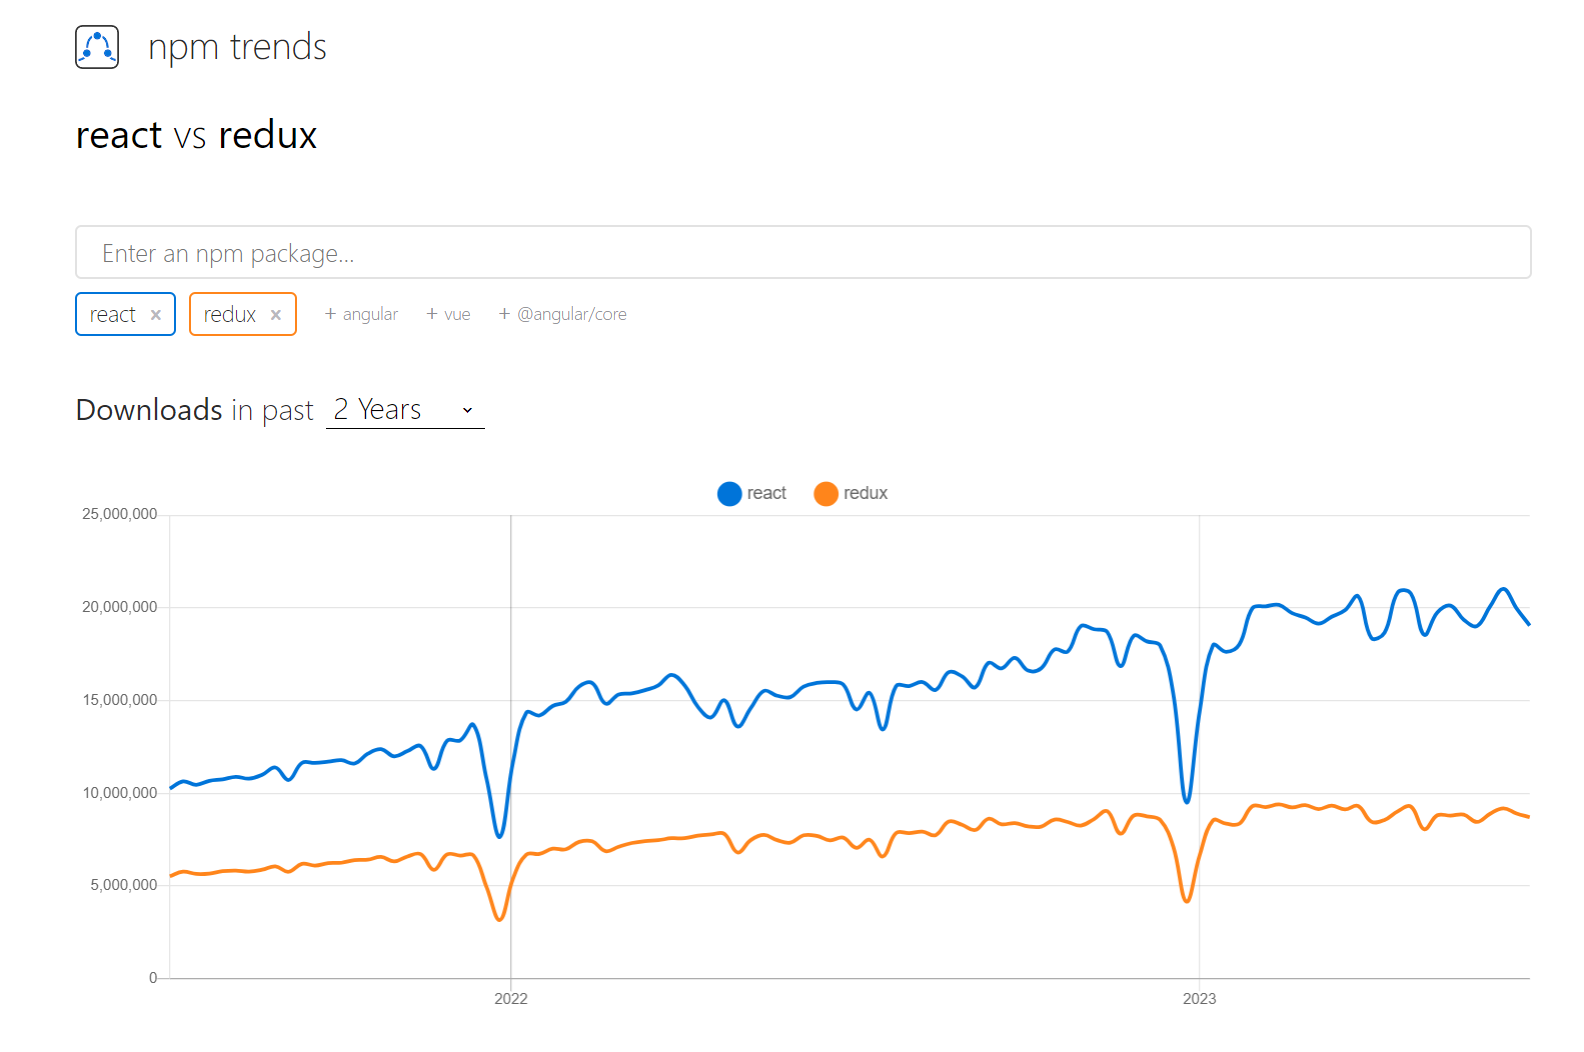
\includegraphics[width=\textwidth]{applied-thesis-chapters/chapter-6/Biểu đồ số lượt tải gói “react” và “redux” theo npm trends trong 2 năm.png}
      \caption{Biểu đồ số lượt tải gói “react” và “redux” theo npm trends từ 7/2021 đến 7/2023}
      \label{fig:BieuDoLuotTai}
\end{figure}

Vì vậy, thư viện Redux thường được chọn để giải quyết vấn đề này cho ứng dụng web được xây dựng với thư viện React.

\myparagraph{Redux Toolkit}
\tab \tab Trong quá khứ, trước phiên bản React 16.8, để có thể theo dõi trạng thái và vòng đời của một thành phần React (React component) thì sử dụng thành phần lớp React (React class component) là cách duy nhất.
Khi đó, việc sử dụng Redux trong ứng dụng React có đôi chút khó khăn và dài dòng do cú pháp, cấu trúc phức tạp.

Từ phiên bản React 16.8, với sự xuất hiện của thành phần hàm React (React functional component) là cách khởi tạo React component mới, cùng với sự xuất hiện của React Hook là cách quản lý trạng thái và vòng đời của component trong React functional component, thì Redux cũng được cải tiến bởi chính nhóm phát triển để phù hợp với sự thay đổi này.
Dẫn đến sự xuất hiện của thư viện Redux Tookit.

\textit{"Redux Toolkit là phương pháp tiêu chuẩn chính thức để viết logic Redux.
      Nó bao bọc xung quanh lõi của Redux, và chứa các gói và hàm được cho là cần thiết để xây dựng một ứng dụng Redux.
      Redux Toolkit tích hợp các thực hành tốt nhất (best practices) được đề xuất, đơn giản hóa hầu hết các tác vụ Redux, ngăn ngừa những sai lầm phổ biến và làm cho việc viết ứng dụng Redux dễ dàng hơn."} \cite{chap4bib1}
\par

\myparagraph{RTK Query}
\tab \tab Khi xây dựng ứng dụng web thì việc tương tác và quản lý dữ liệu API cũng là một vấn đề tiên quyết.
Khi phát triển ứng dụng có sử dụng Redux, nếu muốn đưa dữ liệu nhận được từ API lên trạng thái toàn ứng dụng (global state) thì ta thực hiện chuyển dữ liệu này lên Redux store (đối tượng quản lý global state của Redux).
Redux là một thư viện đồng bộ nhưng tác vụ tương tác với API lại là tác vụ bất đồng bộ, nên thực hiện việc này sẽ có khó khăn là mã dài dòng và khó quản lý lỗi.

Để giải quyết vấn đề này, Redux Tookit có cung cấp hàm createAsyncThunk giúp đơn giản hóa quá trình tạo ra tác vụ bất đồng bộ.
Tuy nhiên, người dùng vẫn phải viết một số lượng logic đáng kể để quản lý dữ liệu ghi đệm và trạng thái tải.
Cũng như khó khăn trong việc quản lý lỗi.
Redux Toolkit Query (RTK Query) là một thư viện bổ sung cho Redux Toolkit.
Cũng được phát triển bởi chính nhóm phát triển thư viện Redux.
Thư viện được phát triển với vai trò như một công cụ tương tác, quản lý dữ liệu khi tương tác với API cho ứng dụng Redux.
\par

\textit{“RTK Query là một công cụ lấy dữ liệu (fetching) và lưu đệm (caching) mạnh mẽ.
      Nó được thiết kế để đơn giản hóa các trường hợp phổ biến khi tải dữ liệu trong một ứng dụng web, loại bỏ nhu cầu viết thủ công các logic lấy dữ liệu và caching của bạn.}
\par

\textit{RTK Query là một addon tùy chọn được bao gồm trong gói Redux Toolkit, và chức năng của nó được xây dựng trên các API khác trong Redux Toolkit.“} \cite{chap4bib2}
\par

Dữ liệu và trạng thái của API được tạo với RTK Query được lưu trữ và quản lý trên store của Redux.
Thiết kế của RTK Query được lấy cảm hứng từ các công cụ phổ biến, tiên phong trong giải pháp lấy dữ liệu API như Apollo Client, React Query, Urql và SWR.
Vậy nên việc sử dụng RTK Query là giải pháp cho tương tác API kết hợp với Redux Tookit trong ứng dụng sẽ giúp cho việc quản lý trạng thái ứng dụng và truy vấn mạng trở nên đơn giản, dễ dàng và hiệu quả hơn.

\subsection{Các chức năng của RTK Query} \label{subsec:CacChucNangRTKQuery}

\tab Thư viện RTK Query hỗ trợ đa dạng chức năng cho truy vấn mạng, tương tác API.
Sau đây là mô tả một số chức năng nổi bật của thư viện RTK Query và có được sử dụng trong phạm vi khóa luận.

\myparagraph{Endpoints, Queries và Mutations}
\tab \tab Việc tương tác với API trong RTK Query xoay quanh việc cài đặt các endpoint.
Endpoint trong RTK Query được định nghĩa trong phương thức createApi() của thư viện.
Phương thức createApi() là chức năng cốt lõi của RTK Query.
Để định nghĩa một endpoint, chúng ta cần cung cấp các thông tin như tên endpoint (là duy nhất trong phạm vi của hàm createApi()) , địa chỉ URL của API, phương thức của endpoint (phương thức HTTP, thông tin này là tùy chọn, mặc định sẽ tùy theo loại endpoint mà ta sử dụng).

Có thể sử dụng các endpoint đã được định nghĩa trong các component của ứng dụng bằng cách sử dụng hook tương ứng.
Các hook này được sinh ra tự động bởi RTK Query và có tên được đặt dựa trên tên của endpoint.
Ví dụ, nếu endpoint được định nghĩa theo loại Query endpoint và có tên là "getUsers", thì hook để sử dụng endpoint này sẽ có tên là "useGetUsersQuery".
Ngoài ra, cũng có thể sử dụng các endpoint  qua đối tượng trả về của hàm createApi(), không qua hook.

Có 2 loại endpoint trong RTK Query là Query endpoint và Mutation endpoint.

\begin{itemize}
      \item \textbf{Query endpoint} khuyến cáo nên được sử dụng khi lấy, truy xuất dữ liệu từ API.
            Khi sử dụng endpoint này, theo mặc định, Query endpoint sẽ tự động thực thi khi component sử dụng nó được hiển thị.
            RTK Query sẽ kiểm tra xem dữ liệu đã được lưu trong store hay chưa.
            Nếu có, dữ liệu đã có trong bộ đệm sẽ được trả về mà không cần gửi yêu cầu đến server.
            Nếu chưa có, yêu cầu sẽ được gửi đến server để lấy dữ liệu mới nhất.
      \item \textbf{Mutation endpoint} khuyến cáo nên được sử dụng khi thay đổi dữ liệu, làm cũ dữ liệu trong store qua API.
            Không như Query endpoint, Mutation endpoint không được thực hiện tự động mà phải gọi tới mỗi khi sử dụng.
            Endpoint này có thể sử dụng để đánh dấu dữ liệu đã cũ trong store, ra hiệu cho các endpoint có liên quan làm mới lại dữ liệu, ví dụ như component có sử dụng Query endpoint sẽ lấy dữ liệu mới, loại bỏ dữ liệu đã cũ trong store.
\end{itemize}

\myparagraph{Các lifecycle hook và Streaming Update}
\tab \tab Endpoint của RTK Query có cung cấp nhiều lifecycle hook mạnh mẽ, hỗ trợ rất nhiều trong việc đóng gói các logic đi kèm bên trong chính endpoint đó.
Các lifecycle hook tiêu biểu được cung cấp trong cả Query endpoint và Mutation endpoint là transformResponse,  transformErrorResponse, onQueryStarted và onCacheEntryAdded.
Đặc biệt, trong Query endpoint có cung cấp hook providesTags và trong Mutation endpoint có cung cấp hook invalidatesTags.
Chi tiết của các hook này như sau:

\begin{itemize}
      \item \textbf{transformResponse:} dùng để cài đặt thay đổi, biến đổi dữ liệu (data) được trả về.
            Dữ liệu được trả về phải đi qua hook này trước khi được lấy ra từ endpoint.
      \item \textbf{transformErrorResponse:} tương tự như transformResponse nhưng dành cho đối tượng lỗi (error).
      \item \textbf{onQueryStarted:} đây là một hook bất đồng bộ, các cài đặt trong hook này sẽ được thực hiện trước khi request của endpoint được gửi đi. Hook này có cung cấp đối tượng LifecycleApi chứa các phương thức để tương tác với dữ liệu, tham số từ endpoint.
      \item \textbf{onCacheEntryAdded:} đây cũng là một hook bất đồng bộ, các cài đặt trong hook sẽ được thực hiện khi có một mục đệm (cache entry) được thêm vào.
            Cache entry là một bộ dữ liệu của một endpoint với tham số truyền vào query đó.
            
            Như đã nói, RTK Query cache dữ liệu của endpoint để tối ưu số lần request, nên nếu có nhiều nơi gọi đến cùng một bộ endpoint và tham số thì dữ liệu sẽ được chia sẻ cho nhau.
            Theo như cài đặt, lần đầu tiên bộ endpoint và tham số được gọi là lần cache entry được thêm vào.
            
            Hook này có cũng cấp đối tượng CacheLifecycleApi có tác dụng tương tự với LifecycleApi từ onQueryStarted.
            CacheLifecycleApi còn có cung cấp thêm 2 thuộc tính là cacheDataLoaded và cacheDataRemoved để hỗ trợ ta có thể cài đặt đồng bộ trong hook.
      \item \textbf{providesTags:} Hook chỉ tồn tại trong Query endpoint.
            Hook giúp cho các Query endpoint tự động làm mới dựa trên các thẻ (tag) mà ta gắn vào.
      \item \textbf{invalidatesTags:} Hook chỉ tồn tại trong Mutation endpoint.
            Hook giúp xác định cache data nào sẽ được tìm nạp lại hoặc xóa khỏi store.
            Khi Mutation endpoint có gắn tag được gọi, dữ liệu nằm trong Query endpoint có tag tương tự sẽ bị đánh dấu là đã cũ.
            Nếu Query endpoint có dữ liệu đã bị đánh dấu cũ thì endpoint đó sẽ được thực hiện gọi lại để làm mới dữ liệu.
\end{itemize}

Trong onQueryStarted và onCacheEntryAdded của Query endpoint, 2 đối tượng LifecycleApi và CacheLifecycleApi đều có cung cấp thêm thuộc tính updateCachedData.
updateCachedData hoạt động như một hàm hỗ trợ việc cập nhật dữ liệu lên đối tượng data của endpoint.
updateCachedData thay đổi dữ liệu giống với cách reducer của Redux.
\par

Có thể điều chỉnh cấu hình endpoint trong cài đặt hay trên hook để thay đổi hành vi của các endpoint.
Một trong những hành vi tiêu biểu nhóm cần trong phạm vi thực hiện khóa luận là cập nhật dữ liệu liên tục (streaming update).
Ta khởi tạo kết nối socket hay event source trong hook onCachedEntryAdded, phối hợp với sử dụng cacheDataLoaded và cacheDataRemoved để thực hiện hành vi này, chi tiết như đoạn trích ở dưới.
\par

\textit{“… bạn sẽ await cacheDataLoaded để xác định thời điểm dữ liệu đầu tiên được tải xuống, sau đó sử dụng tiện ích (utility) updateCacheData để áp dụng các streaming updates khi nhận được tin nhắn (messages).
      updateCacheData là một callback do Immer cung cấp, nhận bản draft của giá trị cache hiện tại.
      Bạn có thể biến đổi giá trị draft để cập nhật giá trị đó khi cần dựa trên các giá trị nhận được.
      RTK Query sau đó sẽ gửi một hành động áp dụng một bản vá lỗi khác dựa trên những thay đổi đó."} \cite{chap4bib3}

\subsection{Kết hợp Redux Toolkit và RTK Query}

\tab Như đã biết, RTK Query là một phần mở rộng của Redux Toolkit, vậy nên ta có thể sử dụng phối hợp RTK Query với Redux Toolkit.
Tiêu biểu là sự kết hợp của extraReducers của Redux Toolkit và các Matchers của RTK Query.
Mô tả của extraReducers và Matchers như sau:

\begin{itemize}
      \item \textbf{ExtraReducers:} Các reducer là một phần quan trọng của kiến trúc Redux.
      Reducer là hàm xử lý lấy trạng thái (state) hiện tại trong Redux store, thực hiện sự kiện (action) và trả về state mới.
      
      Trong Redux Toolkit, tiêu chuẩn để cài đặt Redux logic hoàn chỉnh là thông qua phương thức createSlice() của thư viện.
      Đối tượng thu được của phương thức gọi là slice.
      Trong phương thức createSlice(), ta cài đặt các reducer bên trong thuộc tính "reducers" của phương thức.
      Các reducer được định nghĩa ở trong slice chỉ có thể sử dụng và tương tác được các trạng thái bên trong slice đó.
      
      Đồng thời, phương thức createSlice() cũng có cung cấp thuộc tính extraReducers hỗ trợ cài đặt các reducer.
      Cách hoạt động của các reducer ở thuộc tính này, có cách hoạt động không giống các reducer bên trong thuộc tính "reducer".
      Các reducer của extraReducers phải lắng nghe action nào đó, và chỉ được gọi thực hiện khi action đó xuất hiện.
      Các action này thuộc các reducer bên ngoài slice, của slice khác hoặc trong store chính.
      
      \item \textbf{Matchers:} Như đã mô tả ở phần Endpoints, Queries và Mutations mục \textit{\ref{subsec:CacChucNangRTKQuery} \nameref{subsec:CacChucNangRTKQuery}}, ta định nghĩa các API bằng cách cài đặt các endpoint trong phương thức createApi() của RTK Query, gọi đối tượng nhận được từ phương thức createApi() là api.
      
      Khi tạo endpoint trong phương thức createApi(), RTK Query ngoài việc phát sinh ra các hook tương ứng để sử dụng endpoint, 
      song song đó còn tạo thêm các dịch vụ API (API service) chứa Redux logic, có thể truy cập các API service này thông qua đối tượng api.
      Các API service này gọi là API Slices.
      
      Từ chính đối tượng api, các API Slices cung cấp cho ta đa dạng các nhóm phương thức hỗ trợ như: Tích hợp với Redux (Redux integration), Tương tác với chính endpoint của đối tượng api (Endpoint interactions), Quản lý mã (Code spitting and generation), Sự kiện nội tại (Internal Actions), sử dụng hook trực tiếp từ đối tượng api và các tiện ích (Utilities).
      
      Ở nhóm phương thức Endpoint interactions có cung cấp các thuộc tính matchPending, matchFulfilled và matchRejected cho mỗi endpoint được định nghĩa trong đối tượng api, nhóm các thuộc tính này gọi là Matchers.
      Các thuộc tính này tương ứng với các action pending, fulfilled và rejected có trong một tác vụ bất đồng bộ trong Redux (gọi là thunk), cũng được dùng để xác định trạng thái của tác vụ bất đồng bộ.
\end{itemize}

Như vậy, ta có thể phối hợp sử dụng các thuộc tính trong nhóm Matchers cùng với extraReducers để thực thi các cài đặt dựa trên trạng thái của endpoint đã cài đặt với RTK Query.

\section{Reactive Programming và RxJS} \label{sec:RxJS}

\subsection{Reactive Programming}

\tab Reactive programming là thuật ngữ chỉ phương pháp xử lý, lập trình với dữ liệu không tuần tự.
Dữ liệu trong reactive programming sẽ được chứa trong một dòng tuần tự (stream) tương tự như hình \textit{\ref{fig:StreamInRP} \nameref{fig:StreamInRP}}.

\begin{figure}[H]
      \centering
      \includegraphics[width=\textwidth]{applied-thesis-chapters/chapter-6/Minh họa Stream trong Reactive Programming.png}
      \caption{Minh họa Stream trong Reactive Programming \cite{chap4bib4}}
      \label{fig:StreamInRP}
\end{figure}

Khi stream nhận vào một gói dữ liệu mới, gói đó sẽ được stream vận chuyển đến các điểm chỉnh sửa (modifier).
Modifier là các phương thức được cài đặt, có nhiệm vụ sẽ tự động chạy hay phản ứng (react) với các gói dữ liệu được đưa vào, chỉnh sửa và đưa lại về stream.
\par

Modifier tự động phản ứng với các gói dữ liệu được stream truyền vào, không cần phải tự gọi các modifier như các logic bình thường nên luồng hoạt động của mô hình này dễ đọc hiểu và nắm bắt.
Trong mô hình này, ta có thể tự định nghĩa thứ tự, logic của các modifier trong stream lúc cài đặt.
Tùy vào thứ tự, cách cài đặt của modifier mà các gói dữ liệu trong stream sẽ được thay đổi khác nhau.

\subsection{RxJS}

\tab RxJS, tên đầy đủ nhưng hiếm khi được gọi là ReactX JS, là một thư viện JavaScript dùng để xử lý event được dùng rất rộng rãi hiện nay.
Thư viện được xây dựng dựa trên khái niệm Reactive Programming, cung cấp một cách tiếp cận đơn giản và mạnh mẽ để xử lý các luồng dữ liệu.
Nó có thể sử dụng JavaScript, không phân biệt ứng dụng web hoặc ứng dụng máy chủ.
\par

\textit{“RxJS kết hợp mẫu Observer (Observer pattern) với mẫu Iterator (Iterator pattern) và lập trình hàm (functional programing) với các bộ sưu tập (collections) để quản lý các chuỗi sự kiện một cách lý tưởng.”} \cite{chap4bib5}
\par

Các khái niệm thiết yếu trong RxJS là: \cite{chap4bib5}

\begin{itemize}
      \item \textbf{Observable:} là một đối tượng đại diện cho một chuỗi các sự kiện hoặc giá trị được phát ra theo thời gian.  Có thể hiểu đây là một stream trong Reactive Programming.
      \item \textbf{Observer:} là một tập hợp các callback lắng nghe các giá trị do Observable cung cấp.
            Có ba loại callback trong đối tượng này, mỗi loại callback sẽ có chức năng khác nhau:
            \begin{itemize}
                  \item next: callback này sẽ phản ứng mỗi khi Observable của nó phát ra gói dữ liệu.
                  \item error: callback này sẽ phản ứng khi luồng logic trong Observable của nó phát ra lỗi, tham số trả về trong callback sẽ là lỗi mà Observable gặp phải.
                  \item complete: callback này sẽ phản ứng khi logic của Observable của nó hoàn thành, không còn gói dữ liệu mới phát ra nữa.
            \end{itemize}
      \item \textbf{Subscription:} là đối tượng đại diện cho quá trình đăng ký (subscribe) và hủy đăng ký (unsubscribe) của các Observer với một Observable.
            Là cách tiếp cận tốt để quản lý các đăng ký và giải phóng tài nguyên.
      \item \textbf{Operators:} là các hàm được sử dụng để thực hiện các thao tác trên các Observable, có thể hiểu đây là các Modifier trên stream.
            Các Operators cho phép ta xử lý các logic phức tạp trong Observable đơn giản, hiệu quả và tiện lợi.
            Các Operators có thể được chia thành 2 loại chính: Operators nối tiếp (Pipeable Operators) và Operators khởi tạo (Creation Operators).
            \begin{itemize}
                  \item \textbf{Pipeable Operators:} sử dụng để thực hiện các thao tác trên Observable.
                        Có thể sử dụng phương thức pipe() kết nối các operator với nhau, tạo ra một chuỗi các operator.
                        Pipeable Operators bao gồm map(), filter(), mergeMap() và nhiều hàm khác.
                  \item \textbf{Creation Operators:} sử dụng để tạo ra một Observable mới.
                        Creation Operators bao gồm of(), from(), interval() và nhiều hàm khác.
            \end{itemize}
      \item \textbf{Subject:} là một loại Observable, tương đương với một EventEmitter, có thể được sử dụng trực tiếp để phát ra các sự kiện hoặc giá trị cho nhiều Observers.
      \item \textbf{Schedulers:} là các bộ điều phối tập trung để kiểm soát các hoạt động đồng thời, có thể hiểu đơn giản là sử dụng để kiểm soát và quản lý các hoạt động thực thi theo thứ tự mong muốn.
            Ngoài ra, có thể sử dụng để xác định các nguồn thực thi, thời điểm thực thi trong các Observable, cho các hoạt động đồng bộ và không đồng bộ.
            Schedulers cung cấp các tính năng như điều khiển tốc độ thực thi các hoạt động, điều chỉnh thời gian đợi giữa các hoạt động, phân tán hoạt động cho các luồng thực thi khác.
            Schedulers được đóng gói thành các loại khác nhau gồm:
            \begin{itemize}
                  \item asapScheduler: dùng để kiểm soát các hoạt động đồng bộ, ưu tiên thực hiện các hoạt động ngay khi có thể.
                  \item queueScheduler: dùng để kiểm soát các hoạt động đồng bộ và không đồng bộ, đưa các hoạt động vào một hàng đợi và thực hiện chúng theo thứ tự.
                  \item asyncScheduler: dùng để kiểm soát các hoạt động không đồng bộ, chạy các hoạt động trong một luồng thực thi riêng biệt.
            \end{itemize}
\end{itemize}

Được phát triển bởi Microsoft, với độ linh hoạt và tính năng mạnh mẽ, RxJS đang trở thành một trong những công cụ quan trọng trong việc xây dựng các ứng dụng web và ứng dụng hiện đại.

\newpage
\section{Giao diện và chức năng của ứng dụng}

\tab Phần này trình bày các giao diện màn hình và chức năng cụ thể của màn hình trong ứng dụng Owlens.
Được trình bày chia làm ba phần là các màn hình bên ngoài ứng dụng (chưa đăng nhập), các màn hình bên trong ứng dụng (đã đăng nhập) và Cấu trúc nội dung các tệp báo cáo.

\subsection{Các màn hình bên ngoài ứng dụng}

\tab Các màn hình bên ngoài ứng dụng gồm 2 màn hình là màn hình Trang chủ và màn hình Trang đăng ký / đăng nhập.

\myparagraph{Trang chủ}
\tab \tab Đầu tiên, khi người dùng truy cập vào tên miền thì màn hình đầu tiên người dùng tiếp cập được là màn hình trang chủ.
Ở đây, người dùng có thể sử dụng chức năng dùng thử quét với ZAP Spider hay tiến đến trang đăng nhập.
Các lỗi và trạng thái khi sử dụng chức năng trên được hiển thị rõ ràng trên màn hình này.
Hình \textit{\ref{fig:ManHinhTrangChu} \nameref{fig:ManHinhTrangChu}} 
thể hiện giao diện màn hình trang chủ và các hình \textit{\ref{fig:ManHinhTrangChuVaChucNangDungThu1} \nameref{fig:ManHinhTrangChuVaChucNangDungThu1}}
, \textit{\ref{fig:ManHinhTrangChuVaChucNangDungThu2} \nameref{fig:ManHinhTrangChuVaChucNangDungThu2}} 
thể hiện giao diện màn hình khi sử dụng chức năng dùng thử quét với ZAP Spider.

\begin{figure}[H]
      \centering
      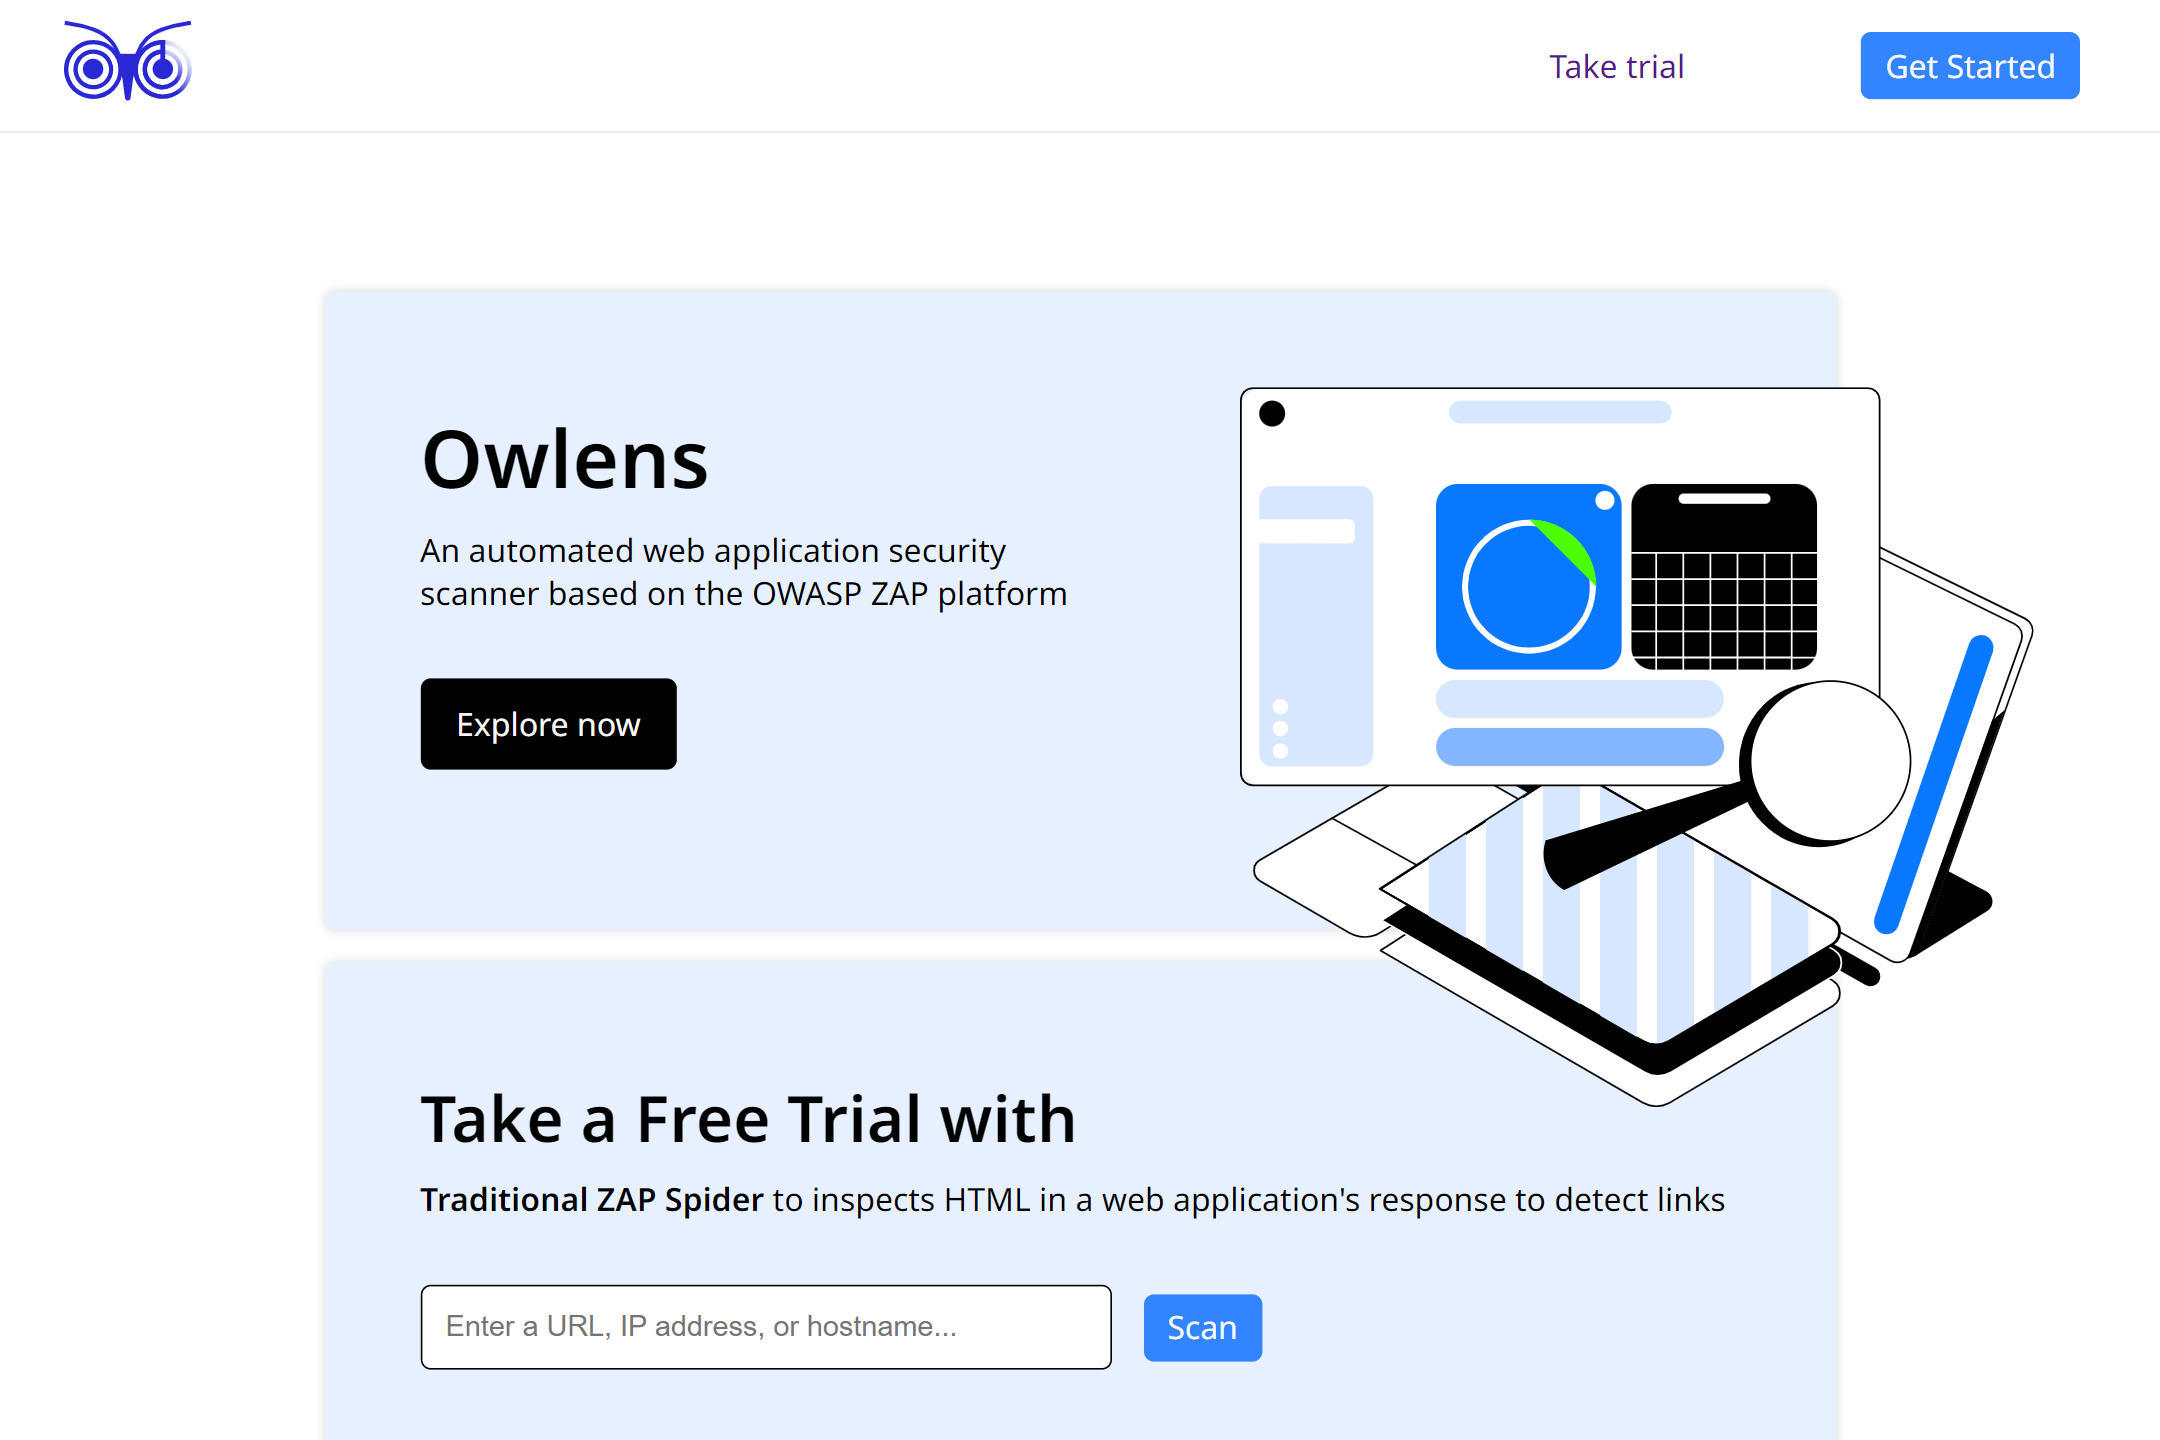
\includegraphics[width=\textwidth]{applied-thesis-chapters/chapter-6/Màn hình trang chủ.png}
      \caption{Màn hình trang chủ}
      \label{fig:ManHinhTrangChu}
\end{figure}

\begin{figure}[H]
      \centering
      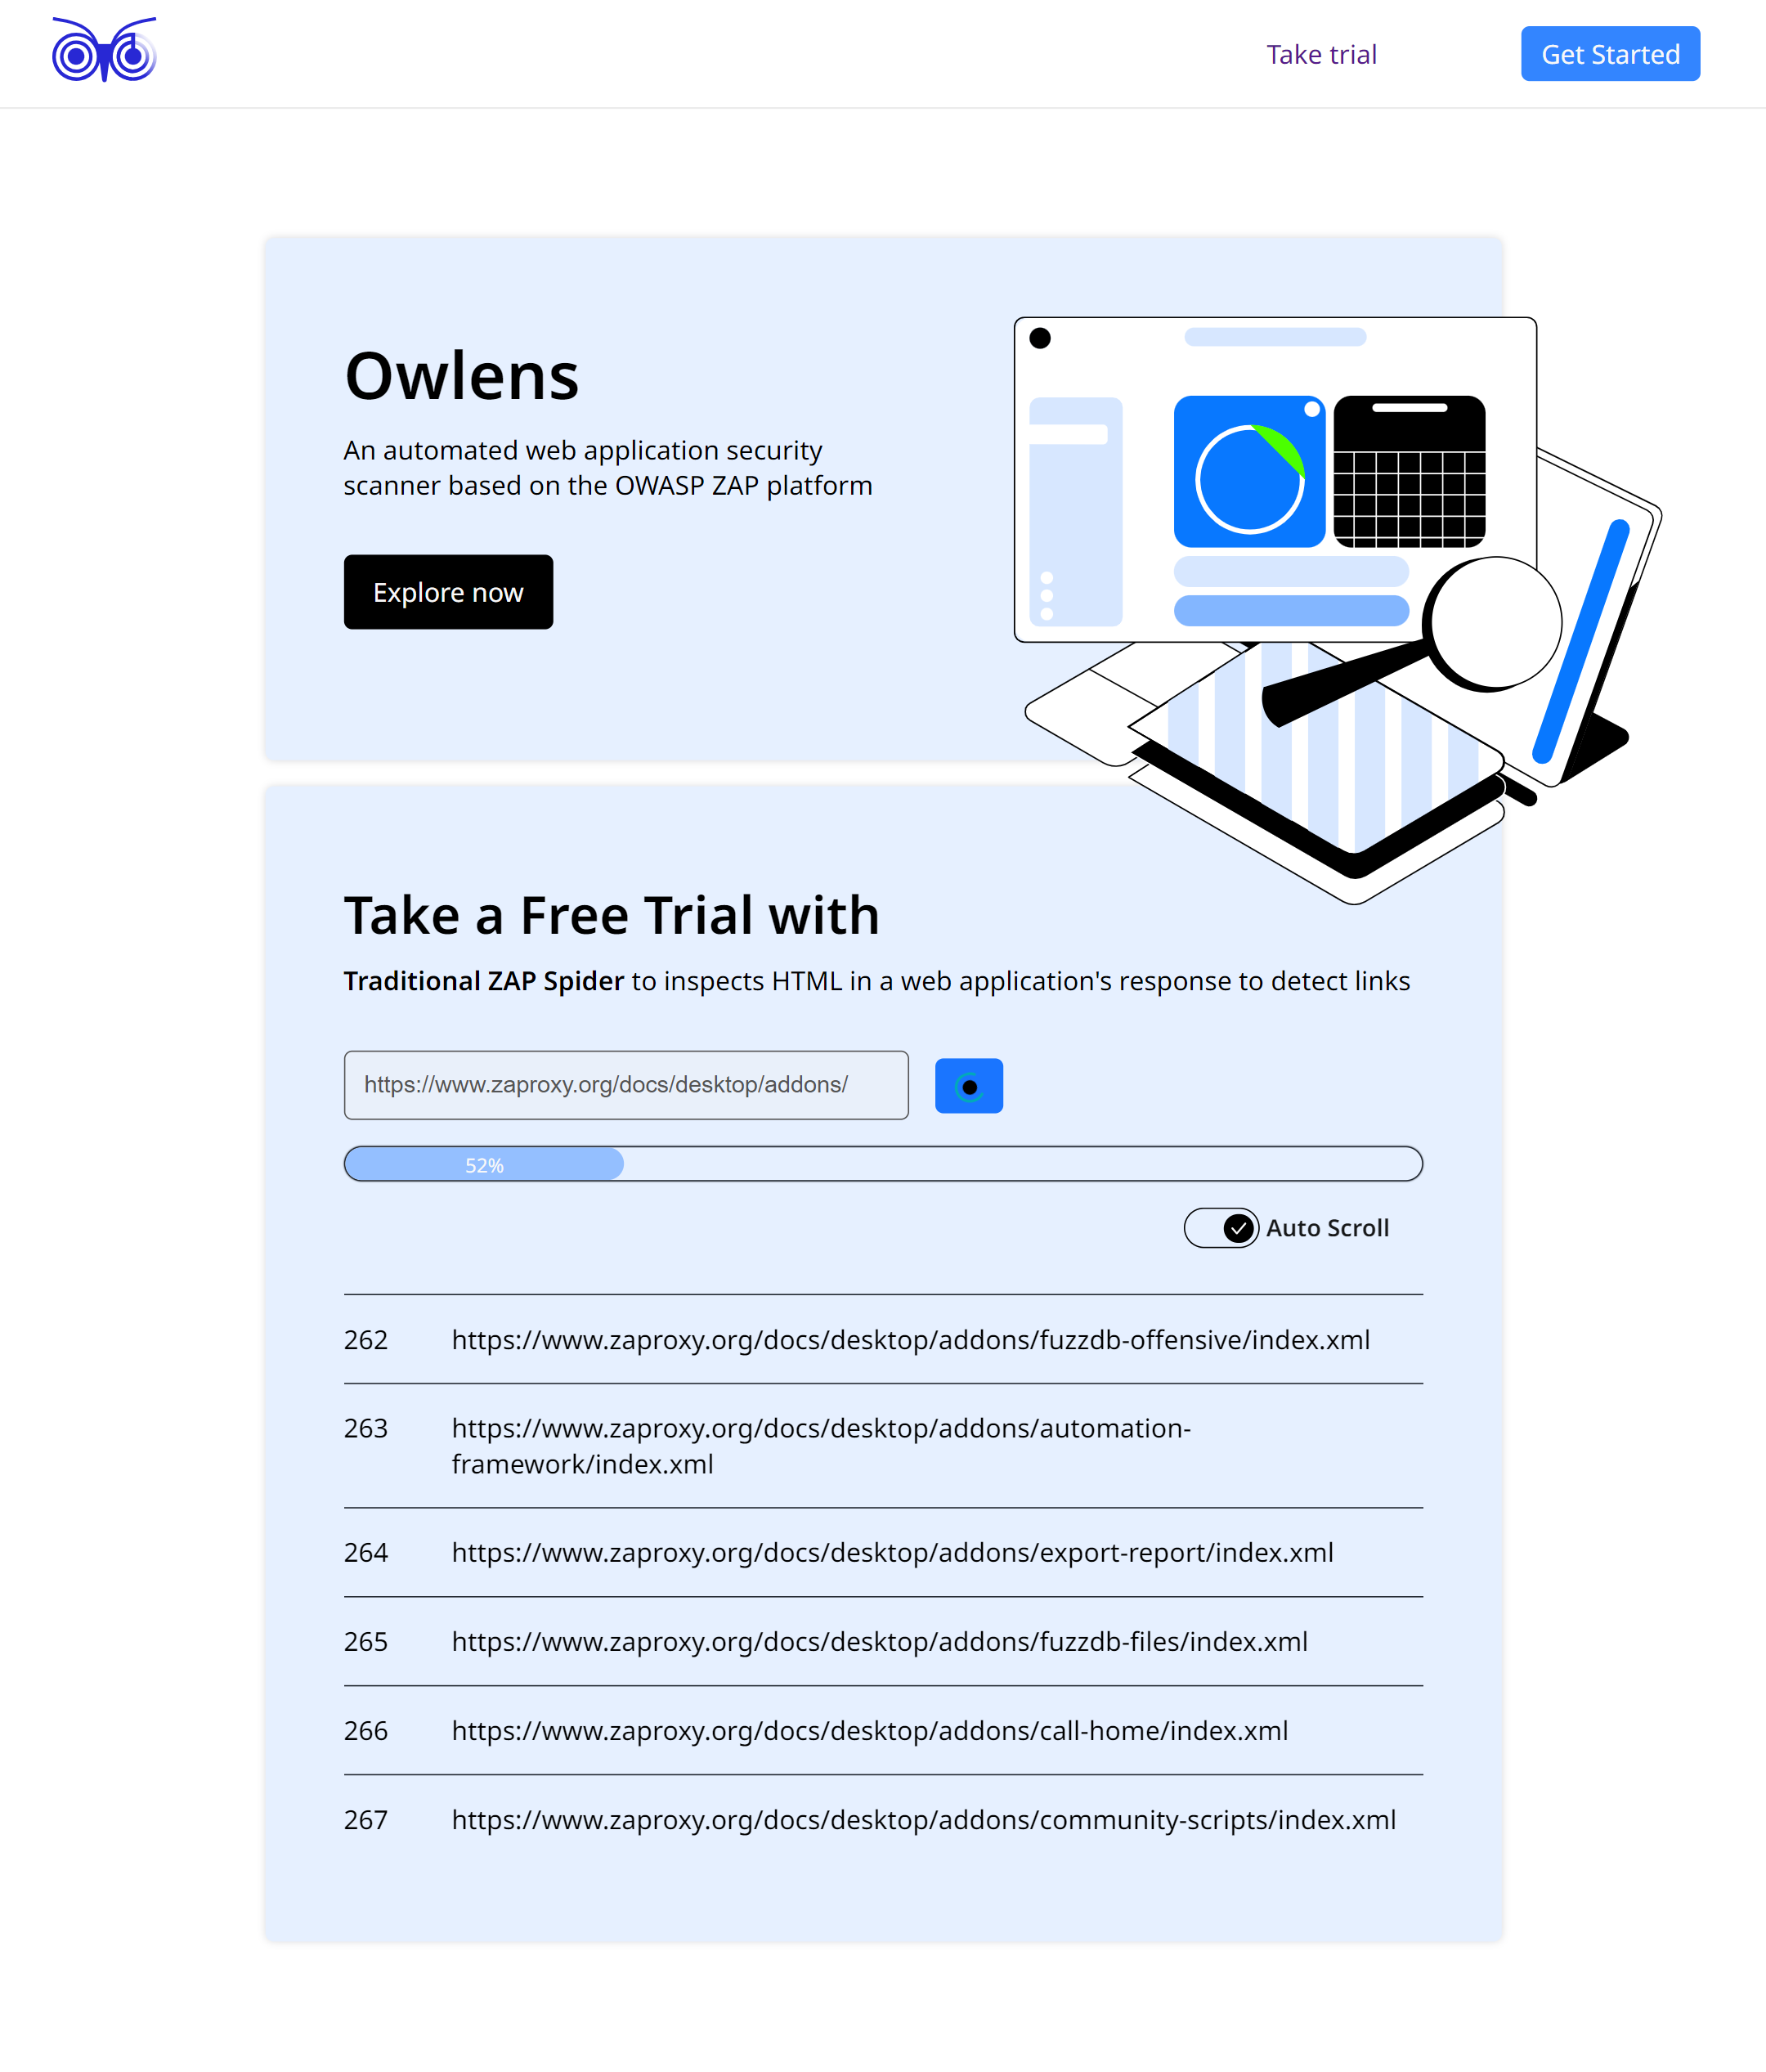
\includegraphics[width=\textwidth]{applied-thesis-chapters/chapter-6/Màn hình trang chủ và chức năng dùng thử 1.png}
      \caption{Màn hình trang chủ và chức năng dùng thử 1}
      \label{fig:ManHinhTrangChuVaChucNangDungThu1}
\end{figure}

\begin{figure}[H]
      \centering
      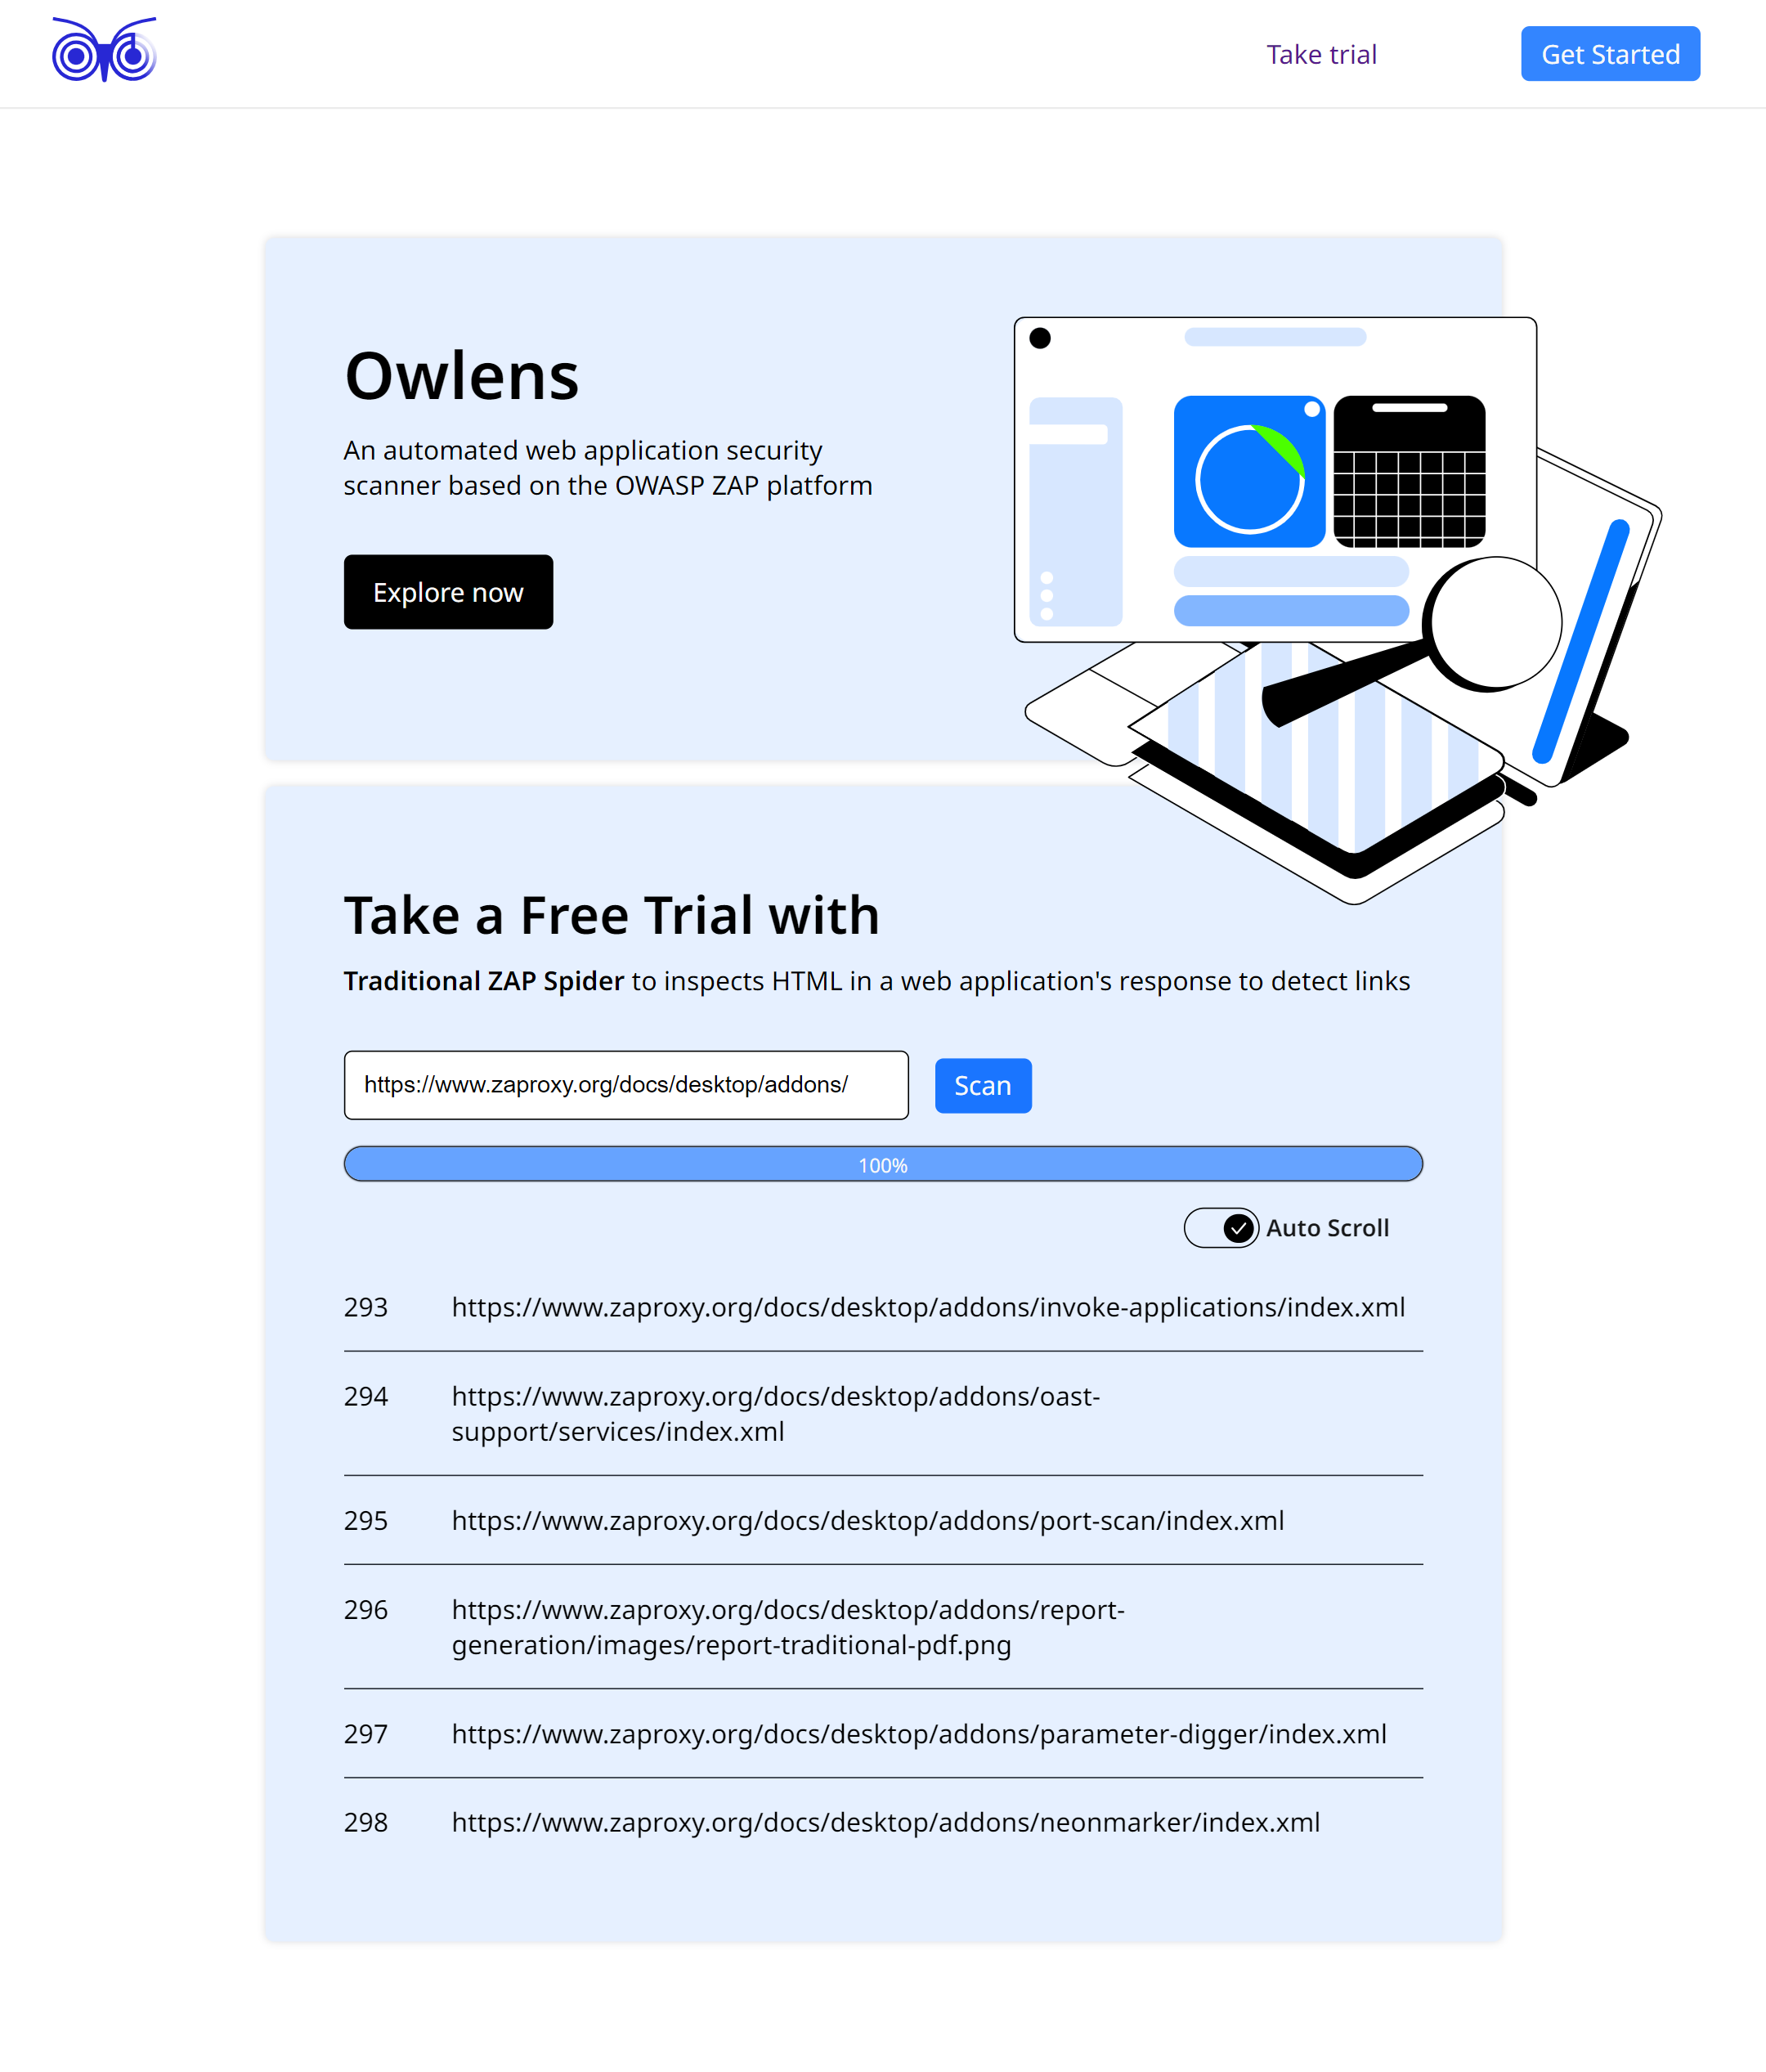
\includegraphics[width=\textwidth]{applied-thesis-chapters/chapter-6/Màn hình trang chủ và chức năng dùng thử 2.png}
      \caption{Màn hình trang chủ và chức năng dùng thử 2}
      \label{fig:ManHinhTrangChuVaChucNangDungThu2}
\end{figure}

\myparagraph{Trang đăng ký / đăng nhập}
\tab \tab Ở màn hình đăng nhập như hình \textit{\ref{fig:ManHinhTrangDangKyDangNhap} \nameref{fig:ManHinhTrangDangKyDangNhap}}, người dùng có thể thực hiện đăng ký / đăng nhập vào ứng dụng web bằng tài khoản Google.
Các trạng thái của quá trình đăng ký / đăng nhập cũng sẽ được thể hiện rõ ràng ở màn hình này.

\begin{figure}[H]
      \centering
      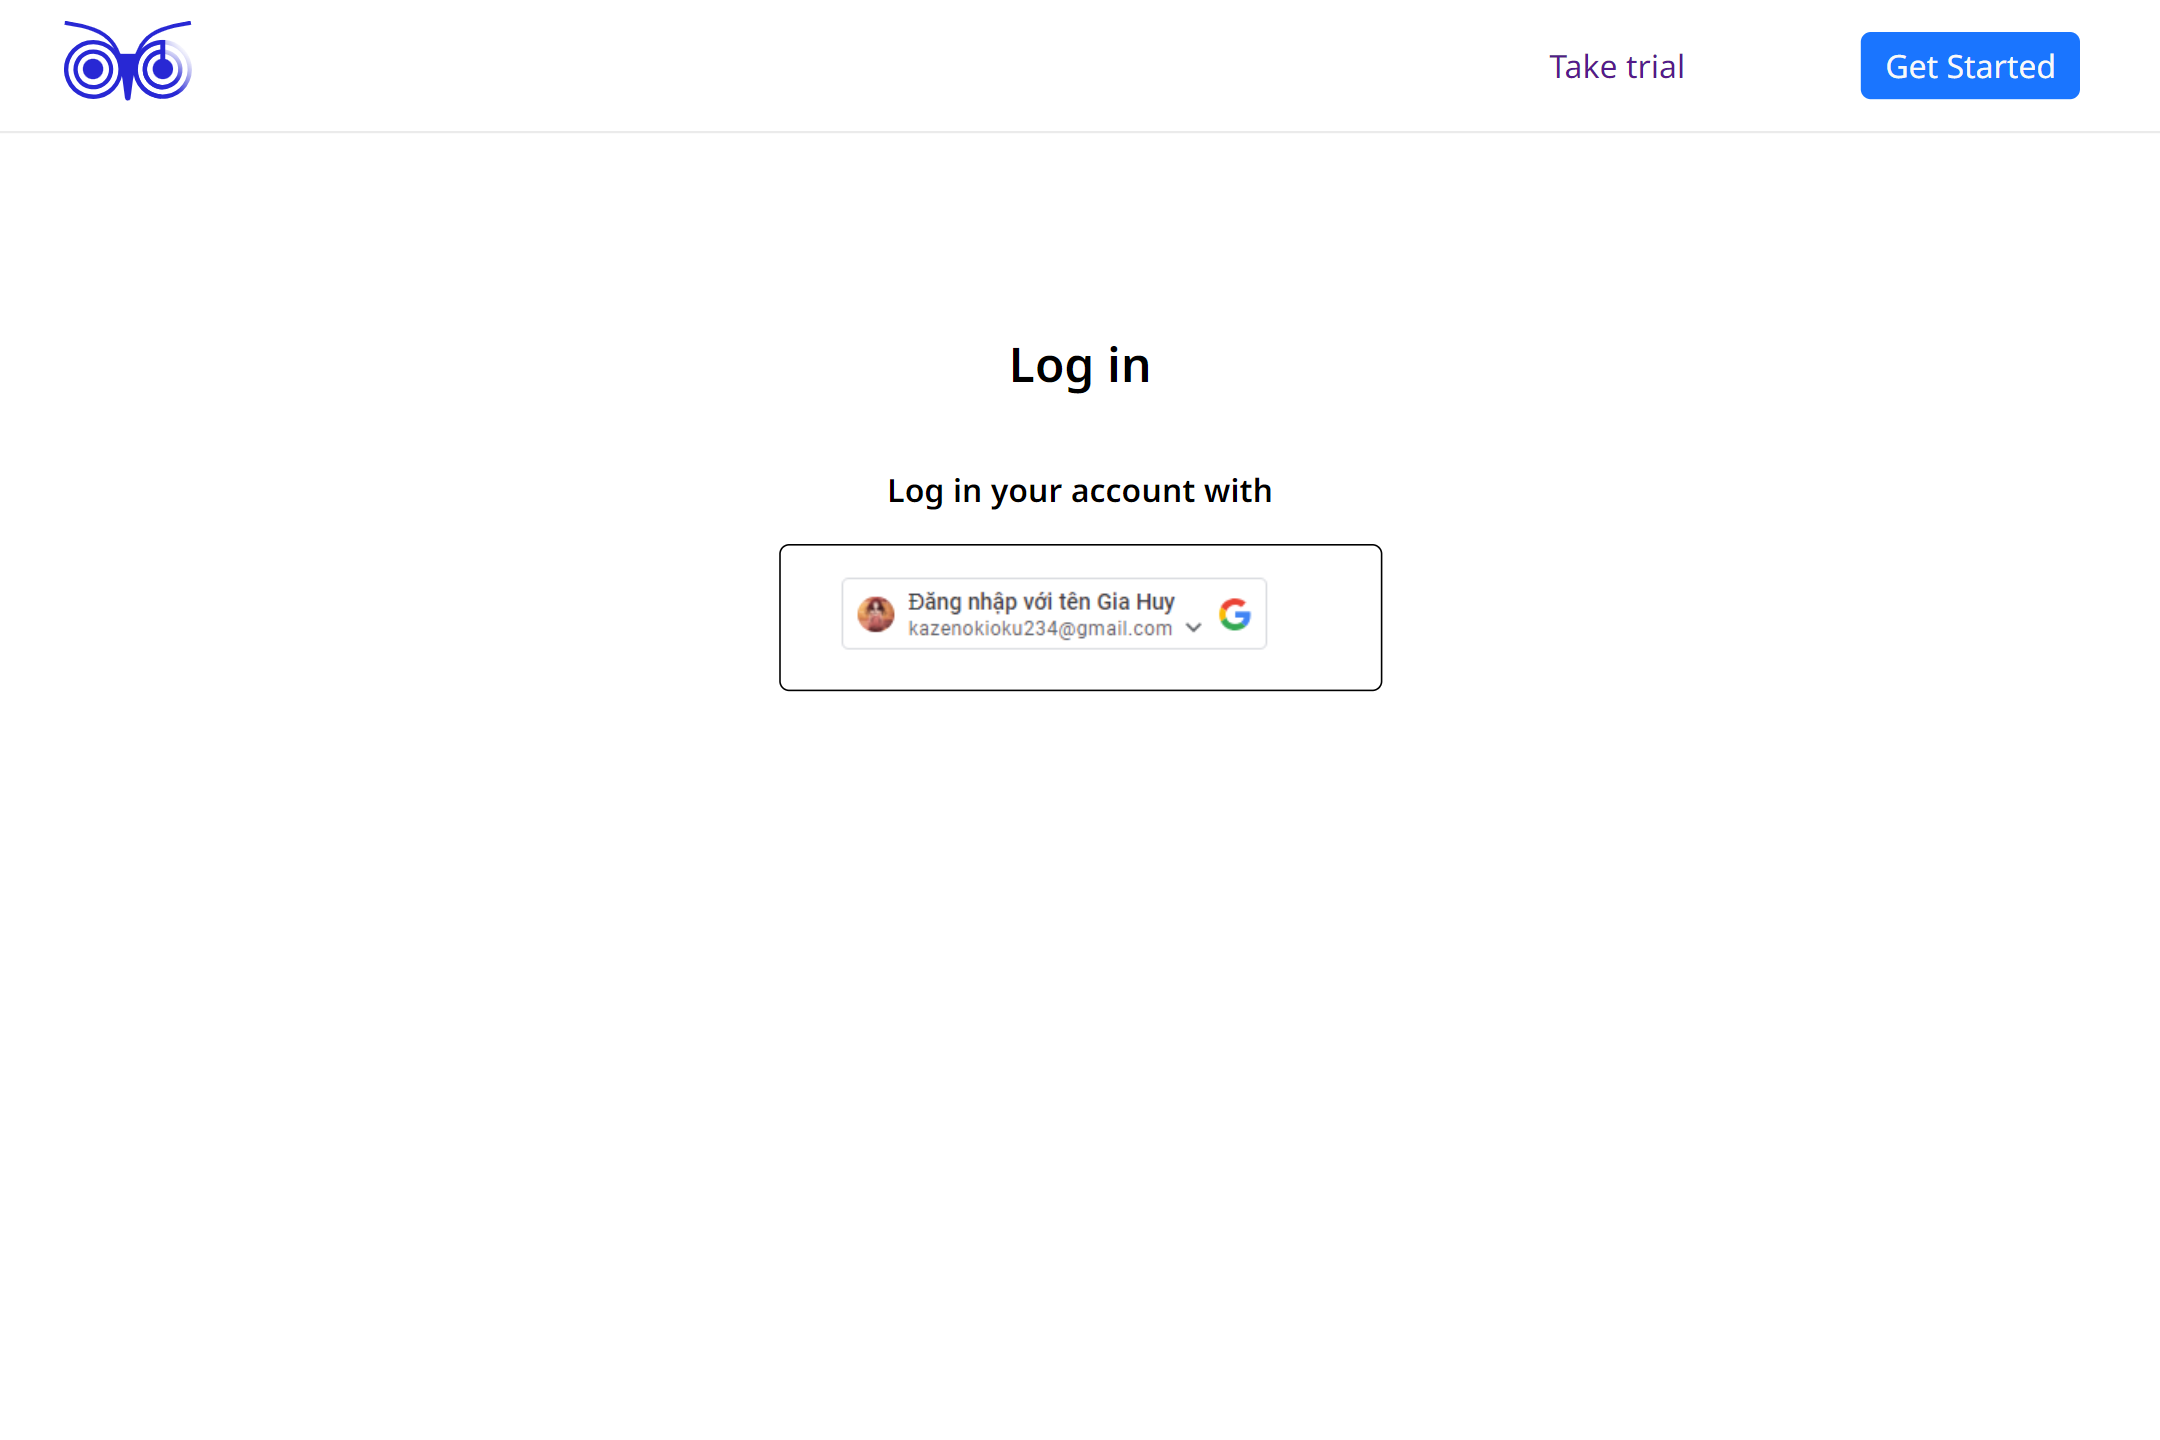
\includegraphics[width=\textwidth]{applied-thesis-chapters/chapter-6/Màn hình trang đăng nhập đăng ký.png}
      \caption{Màn hình trang đăng ký / đăng nhập}
      \label{fig:ManHinhTrangDangKyDangNhap}
\end{figure}

\subsection{Các màn hình bên trong ứng dụng}

\tab Sau khi đăng nhập thành công, người dùng sẽ truy cập vào được màn hình điều khiển ứng dụng.
Màn hình điều khiển ứng dụng được chia làm 5 phần chính Bảng điều khiển (Dashboard), Quản lý mục tiêu (Targets), Quản lý phiên quét (Results), Tạo phiên quét (New scan) và Cài đặt (Settings).

\myparagraph{Bảng điều khiển (Dashboard)}
\tab \tab Hình \textit{\ref{fig:ManHinhDashboard} \nameref{fig:ManHinhDashboard}} thể hiện giao diện phần Dashboard.
Màn hình Dashboard gồm 2 phần là thông tin của phần Targets và Results.

\begin{figure}[H]
      \centering
      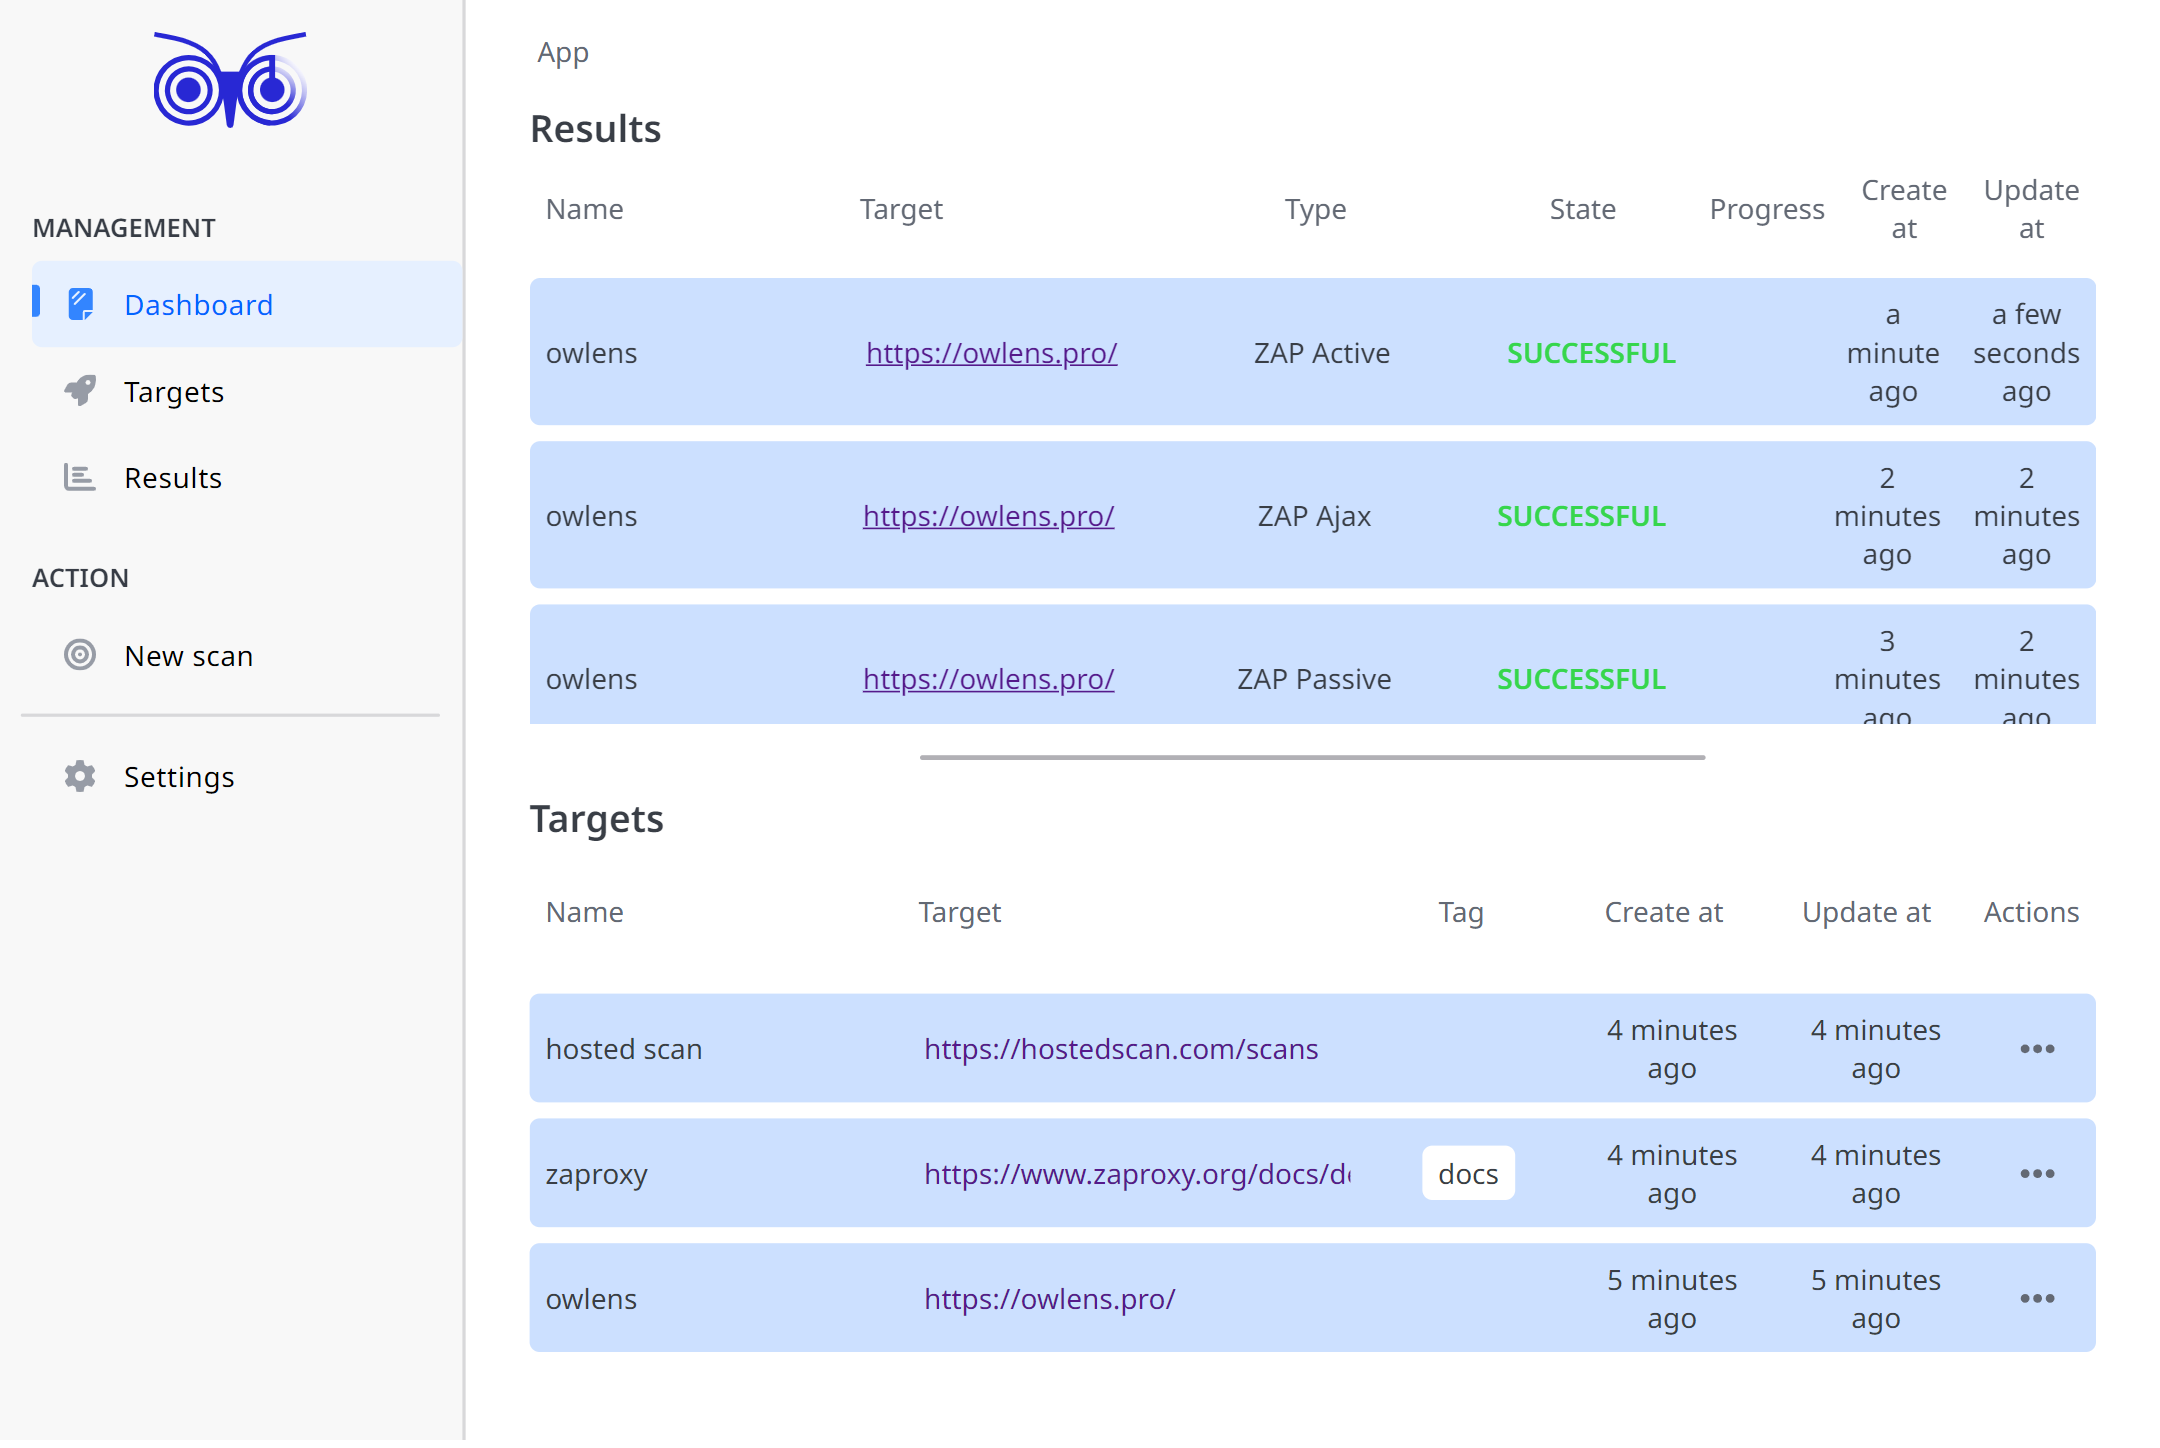
\includegraphics[width=\textwidth]{applied-thesis-chapters/chapter-6/Màn hình Dashboard.png}
      \caption{Màn hình Dashboard}
      \label{fig:ManHinhDashboard}
\end{figure}

Người dùng có thể truy cập, sử dụng nhanh các tác vụ mà không cần đi đến màn hình điều khiển cụ thể của từng phần.
Trong Dashboard, thứ tự hiển thị trên dưới của 2 phần Results và Targets sẽ thay đổi theo thời gian thay đổi dữ liệu nội tại của từng phần.
Ví dụ, nếu dữ liệu của Targets có thay đổi mới gần hơn Results thì phần Targets sẽ được hiển thị bên trên và ngược lại.

\myparagraph{Quản lý mục tiêu (Targets)}
\tab \tab Hình \textit{\ref{fig:ManHinhTargets} \nameref{fig:ManHinhTargets}} thể hiện giao diện phần Targets.
Màn hình Targets thể hiện thông tin và quản lý các mục tiêu.

\begin{figure}[H]
      \centering
      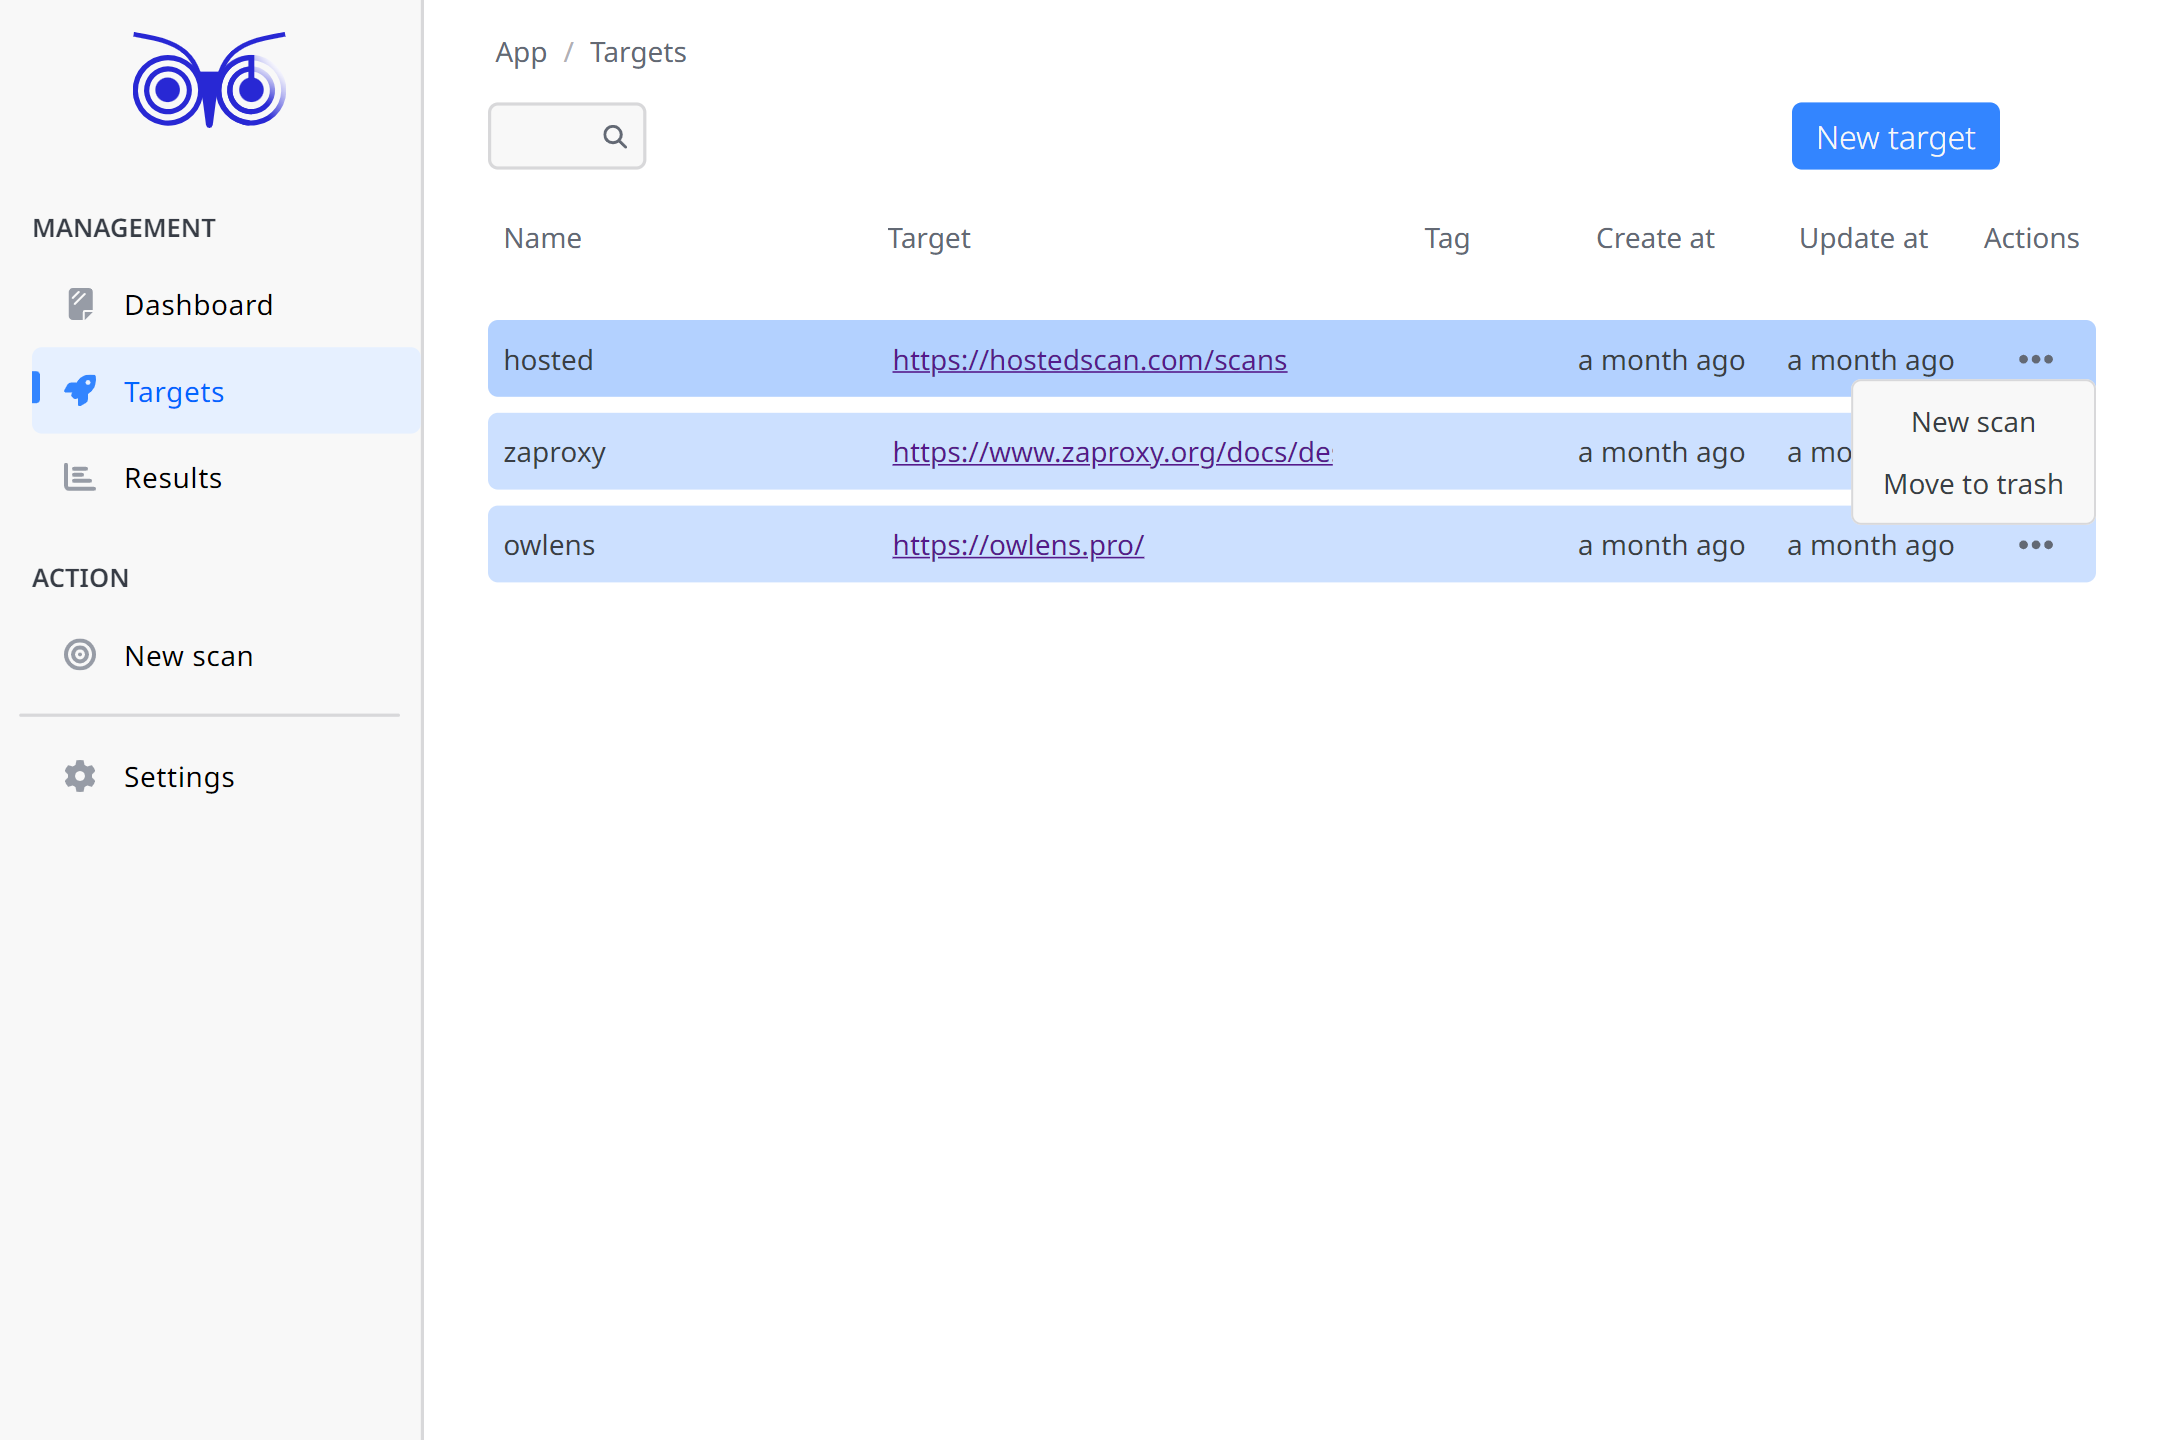
\includegraphics[width=\textwidth]{applied-thesis-chapters/chapter-6/Màn hình Targets.png}
      \caption{Màn hình Targets}
      \label{fig:ManHinhTargets}
\end{figure}

Người dùng có thể xóa mục tiêu và tạo mới phiên quét trong mỗi mục của mục tiêu.
Người dùng cũng thực hiện tạo mới mục tiêu ở đây.

Các hình \textit{\ref{fig:ManHinhTargetsVaThemMoiMucTieu1} \nameref{fig:ManHinhTargetsVaThemMoiMucTieu1}} 
và \textit{\ref{fig:ManHinhTargetsVaThemMoiMucTieu2} \nameref{fig:ManHinhTargetsVaThemMoiMucTieu2}} thể hiện giao diện các màn hình và cửa sổ trong quá trình tạo mới mục tiêu.

\begin{figure}[H]
      \centering
      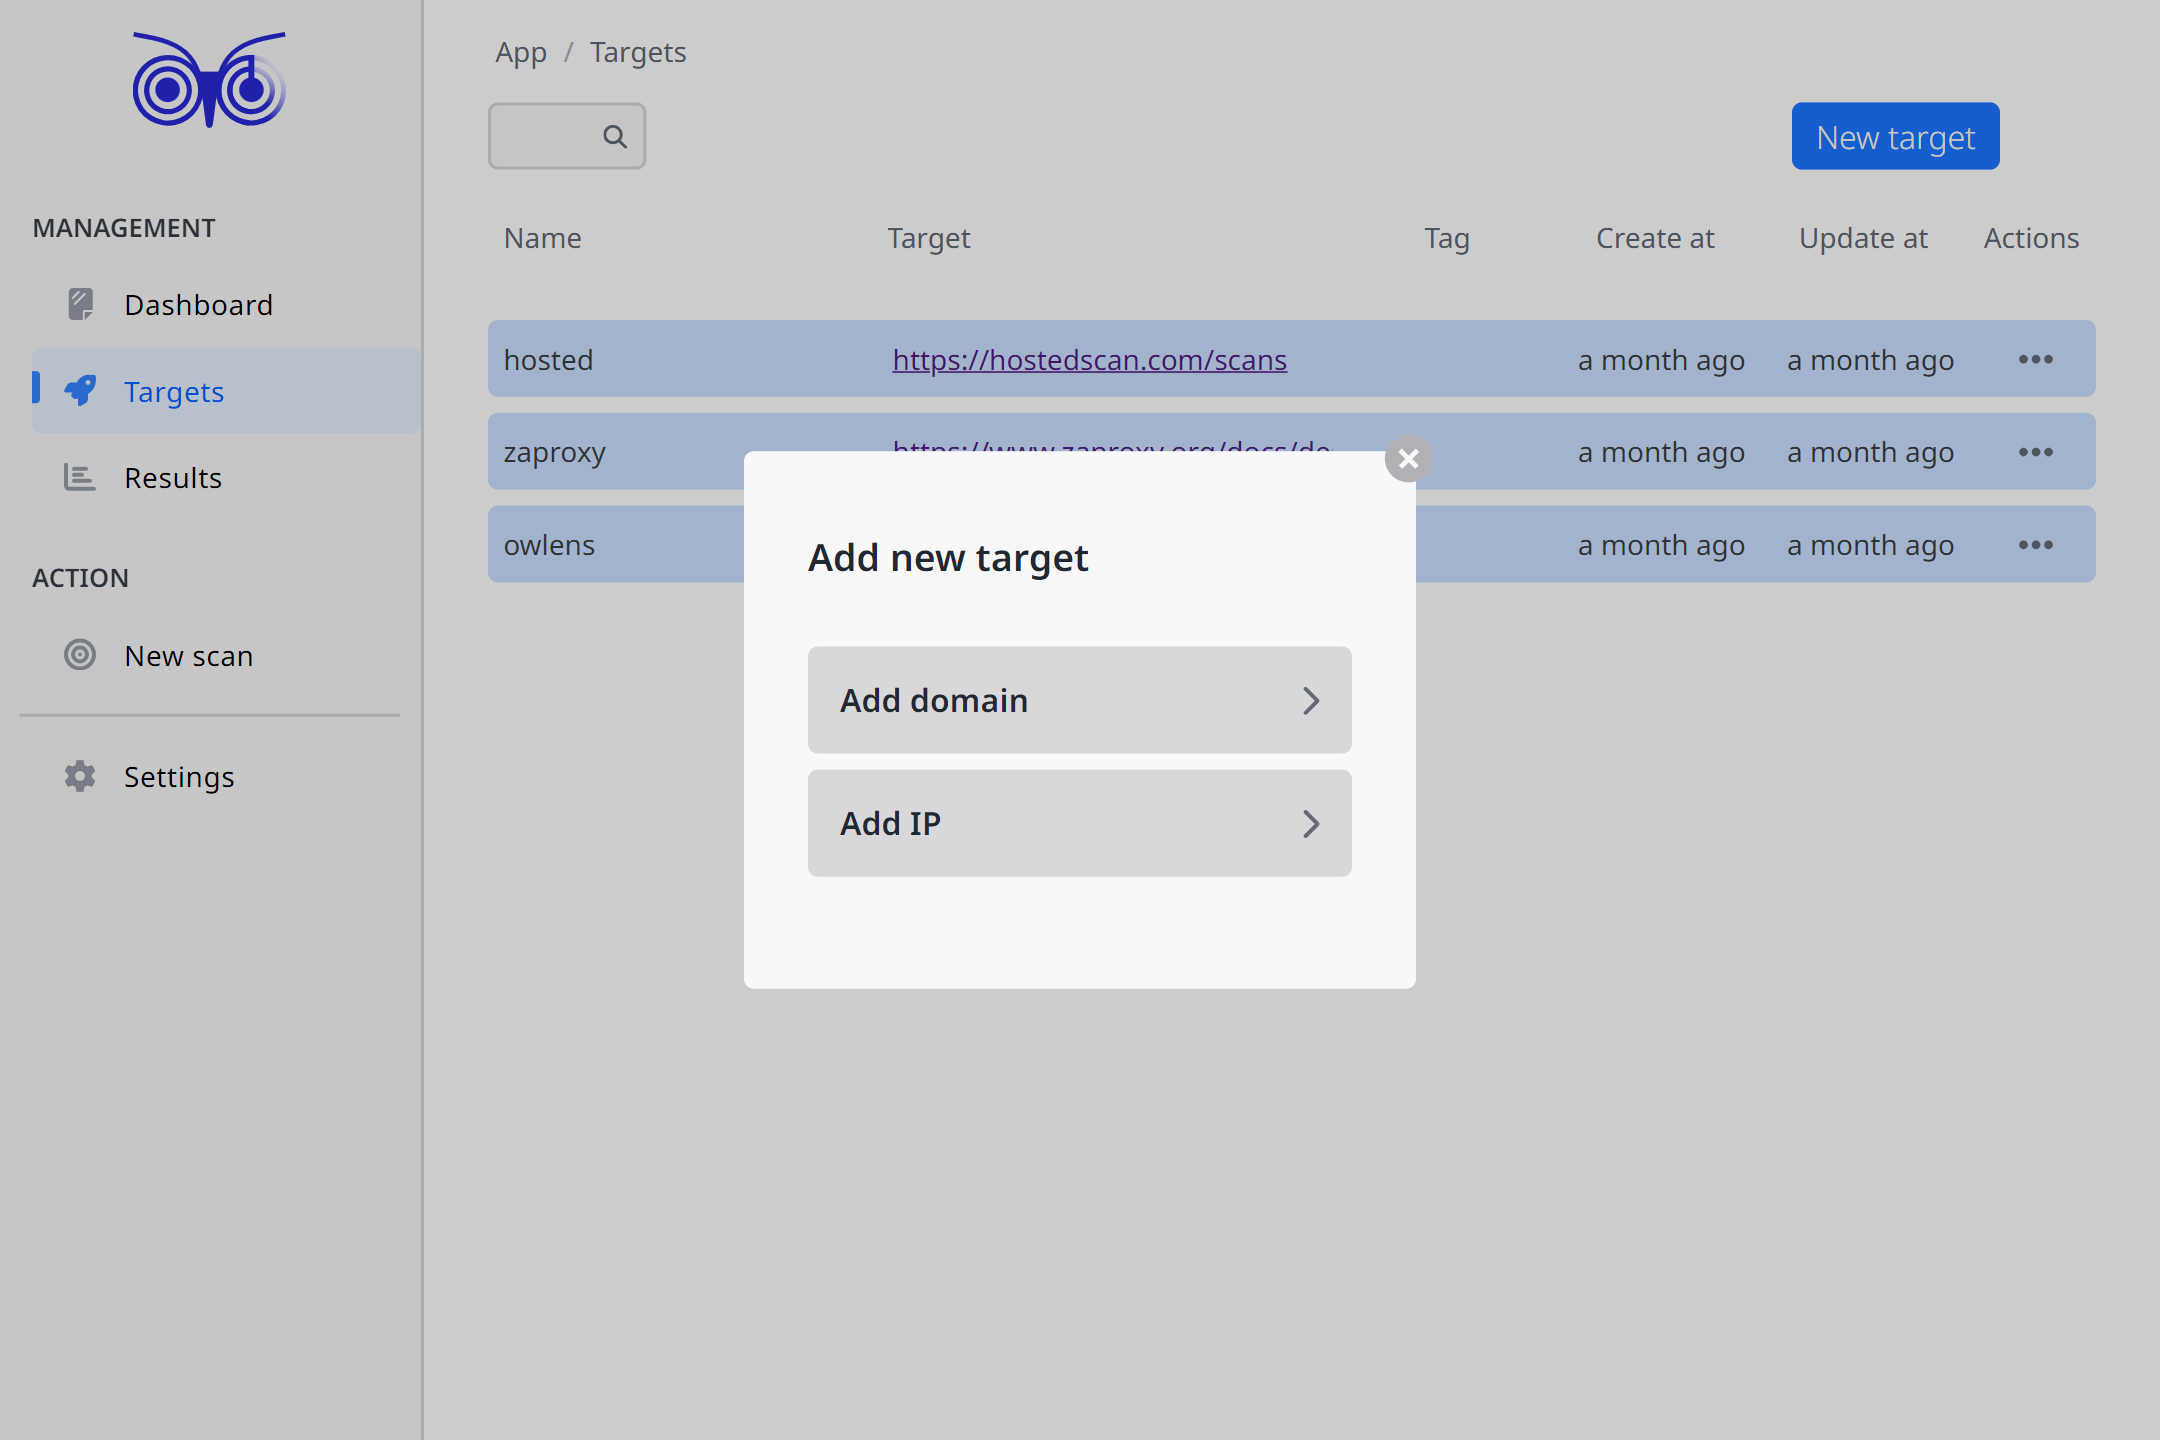
\includegraphics[width=\textwidth]{applied-thesis-chapters/chapter-6/Màn hình Targets và thêm mới mục tiêu 1.png}
      \caption{Màn hình Targets và thêm mới mục tiêu 1}
      \label{fig:ManHinhTargetsVaThemMoiMucTieu1}
\end{figure}

\begin{figure}[H]
      \centering
      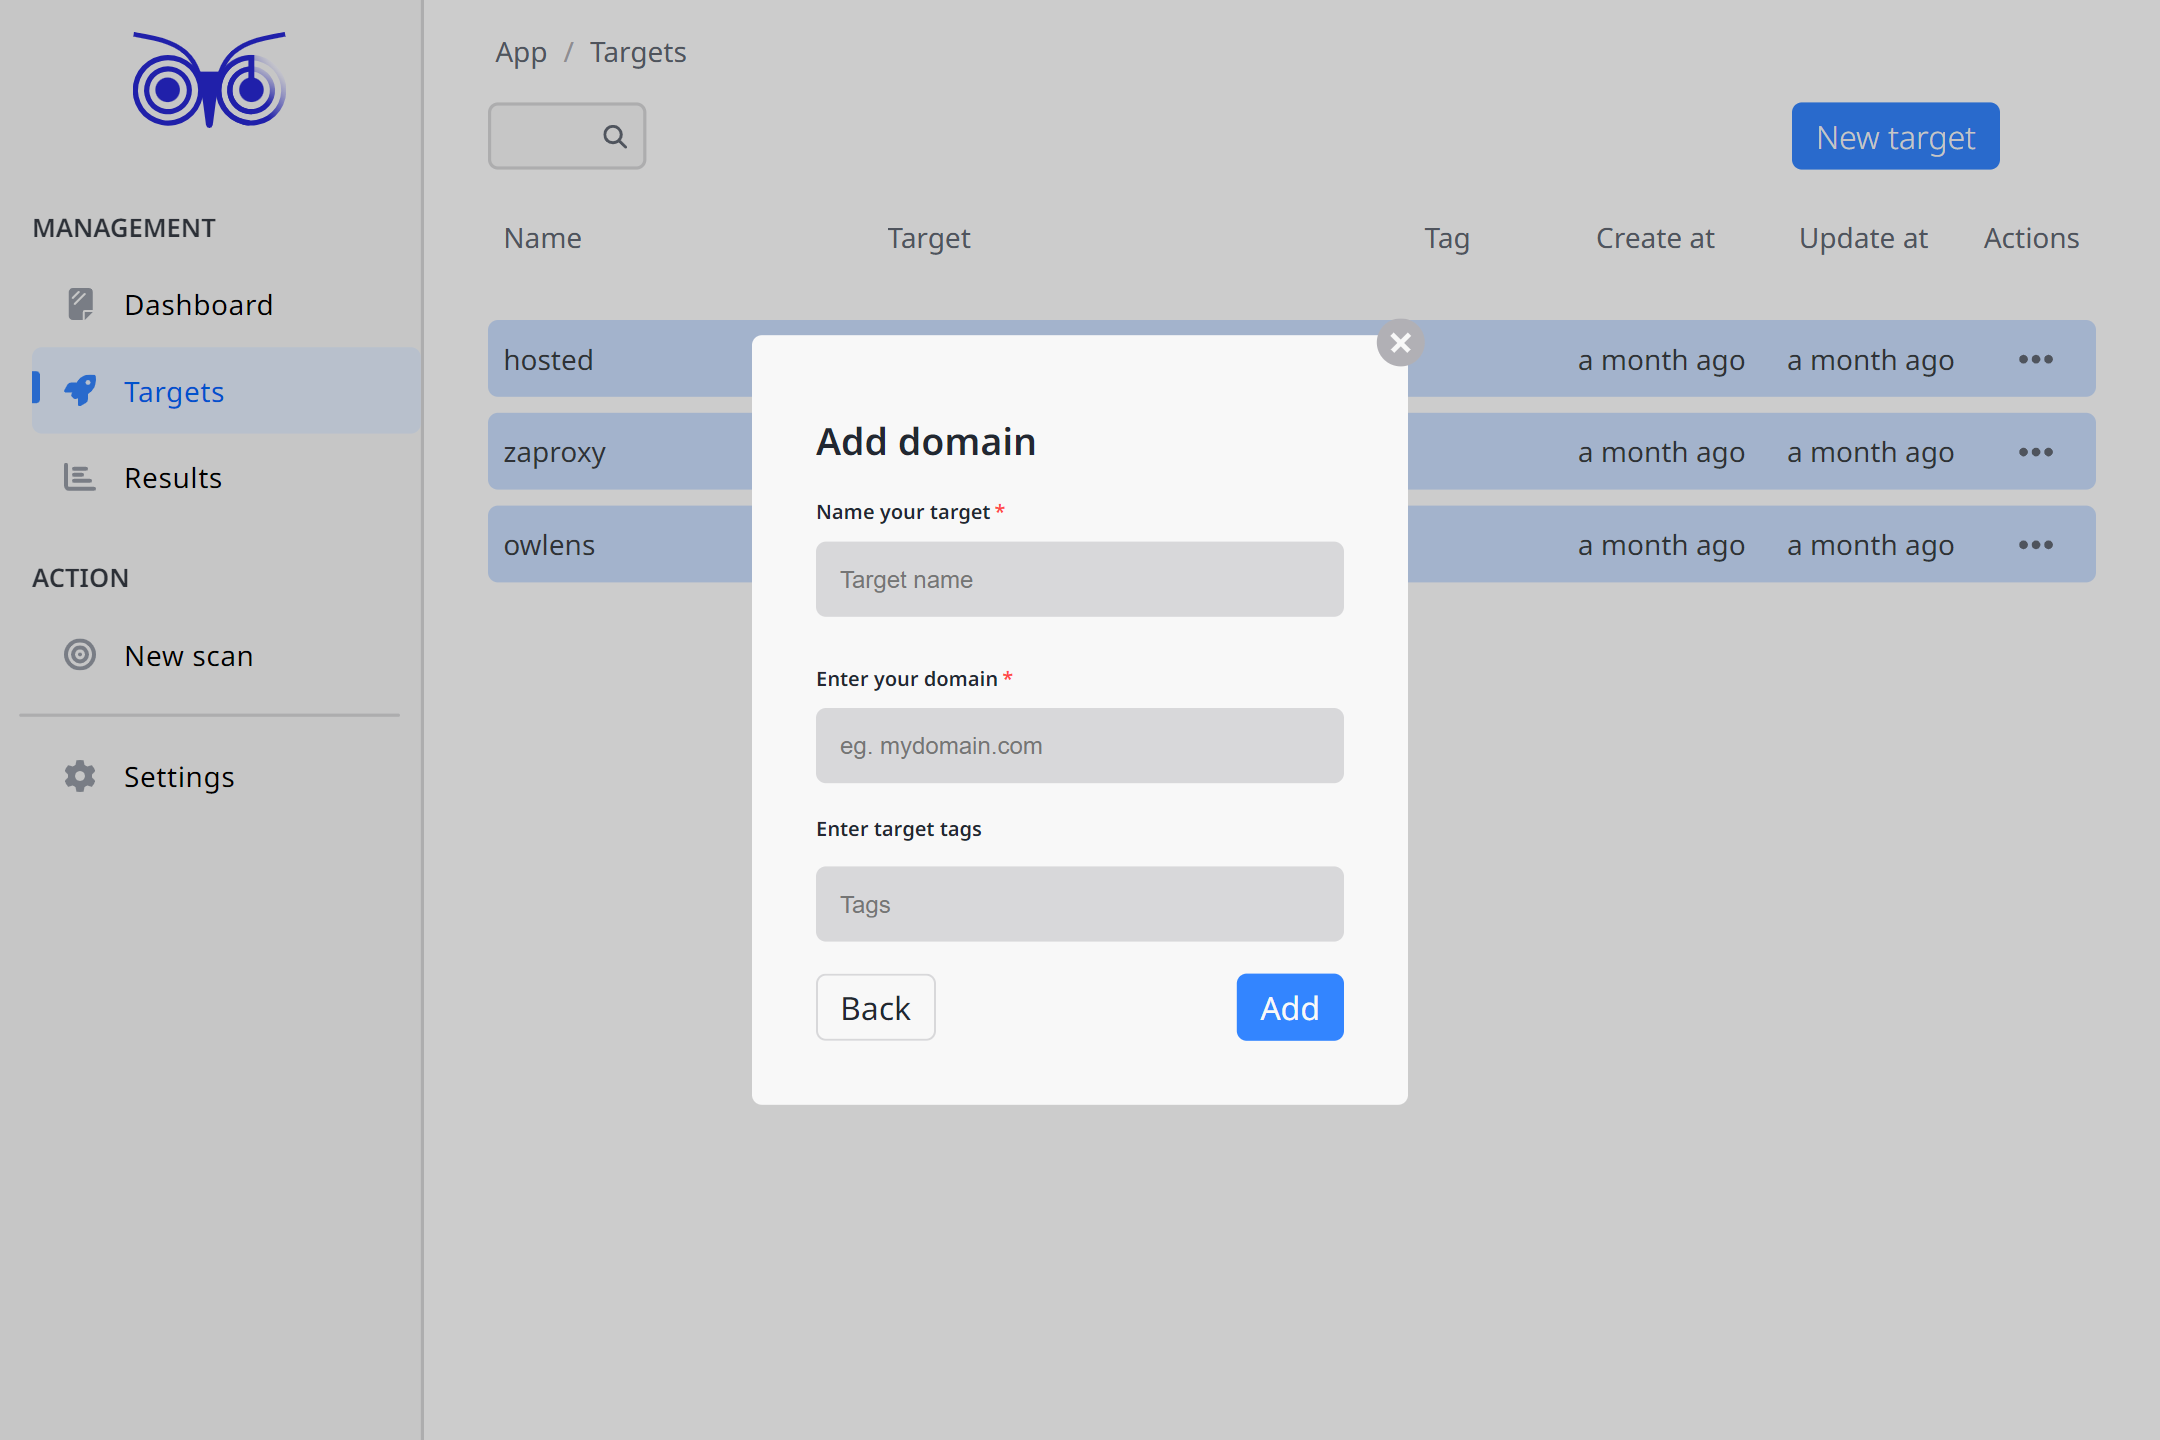
\includegraphics[width=\textwidth]{applied-thesis-chapters/chapter-6/Màn hình Targets và thêm mới mục tiêu 2.png}
      \caption{Màn hình Targets và thêm mới mục tiêu 2}
      \label{fig:ManHinhTargetsVaThemMoiMucTieu2}
\end{figure}

Người dùng có thể tạo mới mục tiêu dạng URL hay IP, giao diện quá trình tạo mới mục tiêu dạng IP cũng tương tự khi thực hiện với URL.
Các thông báo ngoại lệ trong quá trình thêm mới mục tiêu được thể hiện trên cửa sổ thêm mới của màn hình ở hình \textit{\ref{fig:ManHinhTargetsVaThemMoiMucTieu2} \nameref{fig:ManHinhTargetsVaThemMoiMucTieu2}}.

\myparagraph{Quản lý phiên quét (Results)}
\tab \tab Hình \textit{\ref{fig:ManHinhResults} \nameref{fig:ManHinhResults}} thể hiện giao diện phần Results.
Màn hình Results thể hiện thông tin và trạng thái chung của các phiên quét.

\begin{figure}[H]
      \centering
      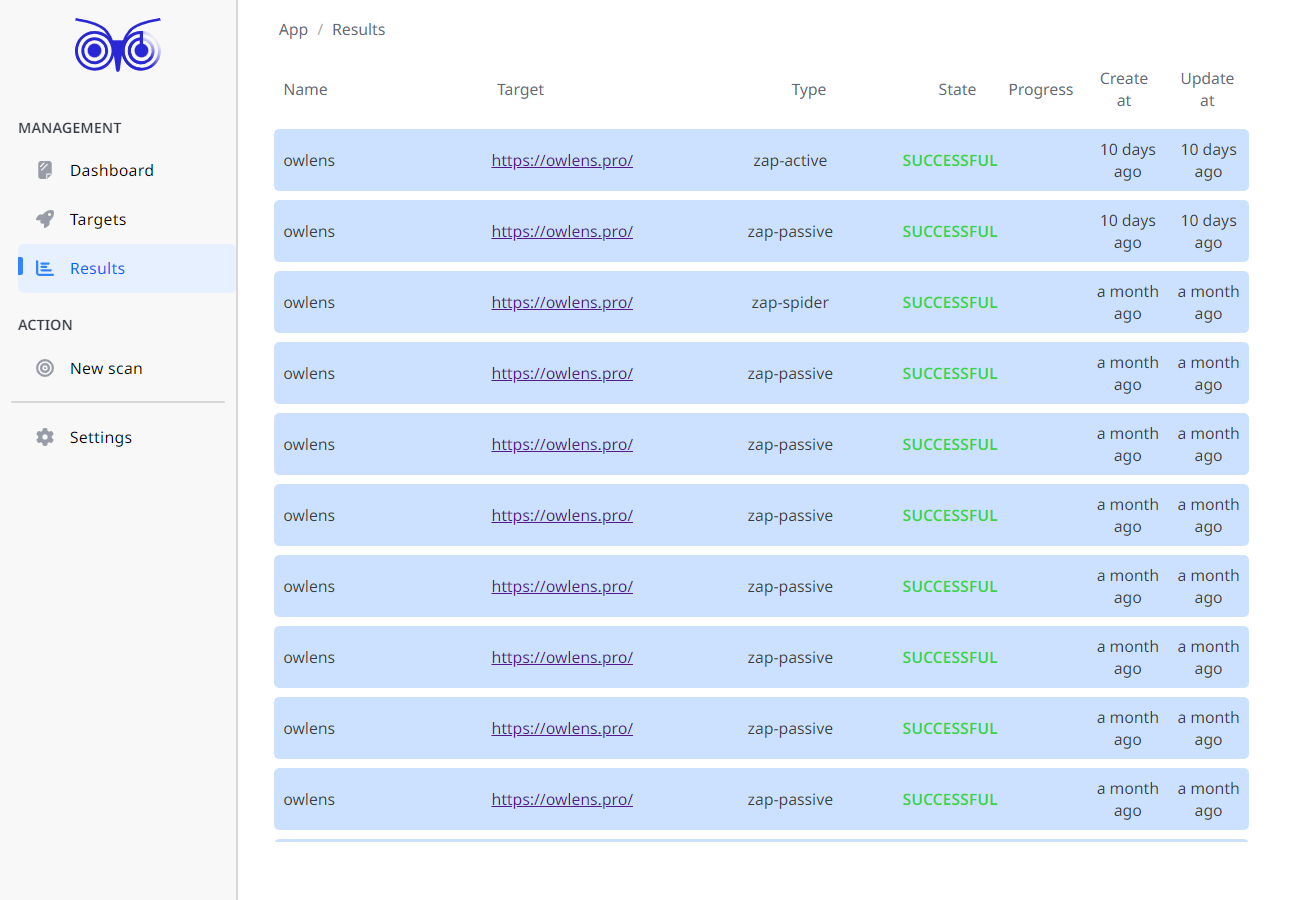
\includegraphics[width=\textwidth]{applied-thesis-chapters/chapter-6/Màn hình Results.png}
      \caption{Màn hình Results}
      \label{fig:ManHinhResults}
\end{figure}

Người dùng truy cập vào màn hình kết quả quét chi tiết của phiên quét bằng cách chọn vào mục của phiên quét.
Mỗi loại quét khác nhau sẽ có giao diện màn hình kết quả quét chi tiết khác nhau.

Các hình \textit{\ref{fig:ManHinhKetQuaQuetChiTietSpiderVaURLsInScope} \nameref{fig:ManHinhKetQuaQuetChiTietSpiderVaURLsInScope}} 
và \textit{\ref{fig:ManHinhKetQuaQuetChiTietSpiderVaURLsOutOfScope} \nameref{fig:ManHinhKetQuaQuetChiTietSpiderVaURLsOutOfScope}} 
thể hiện giao diện màn hình kết quả quét chi tiết của phiên quét loại ZAP Spider.

\begin{figure}[H]
      \centering
      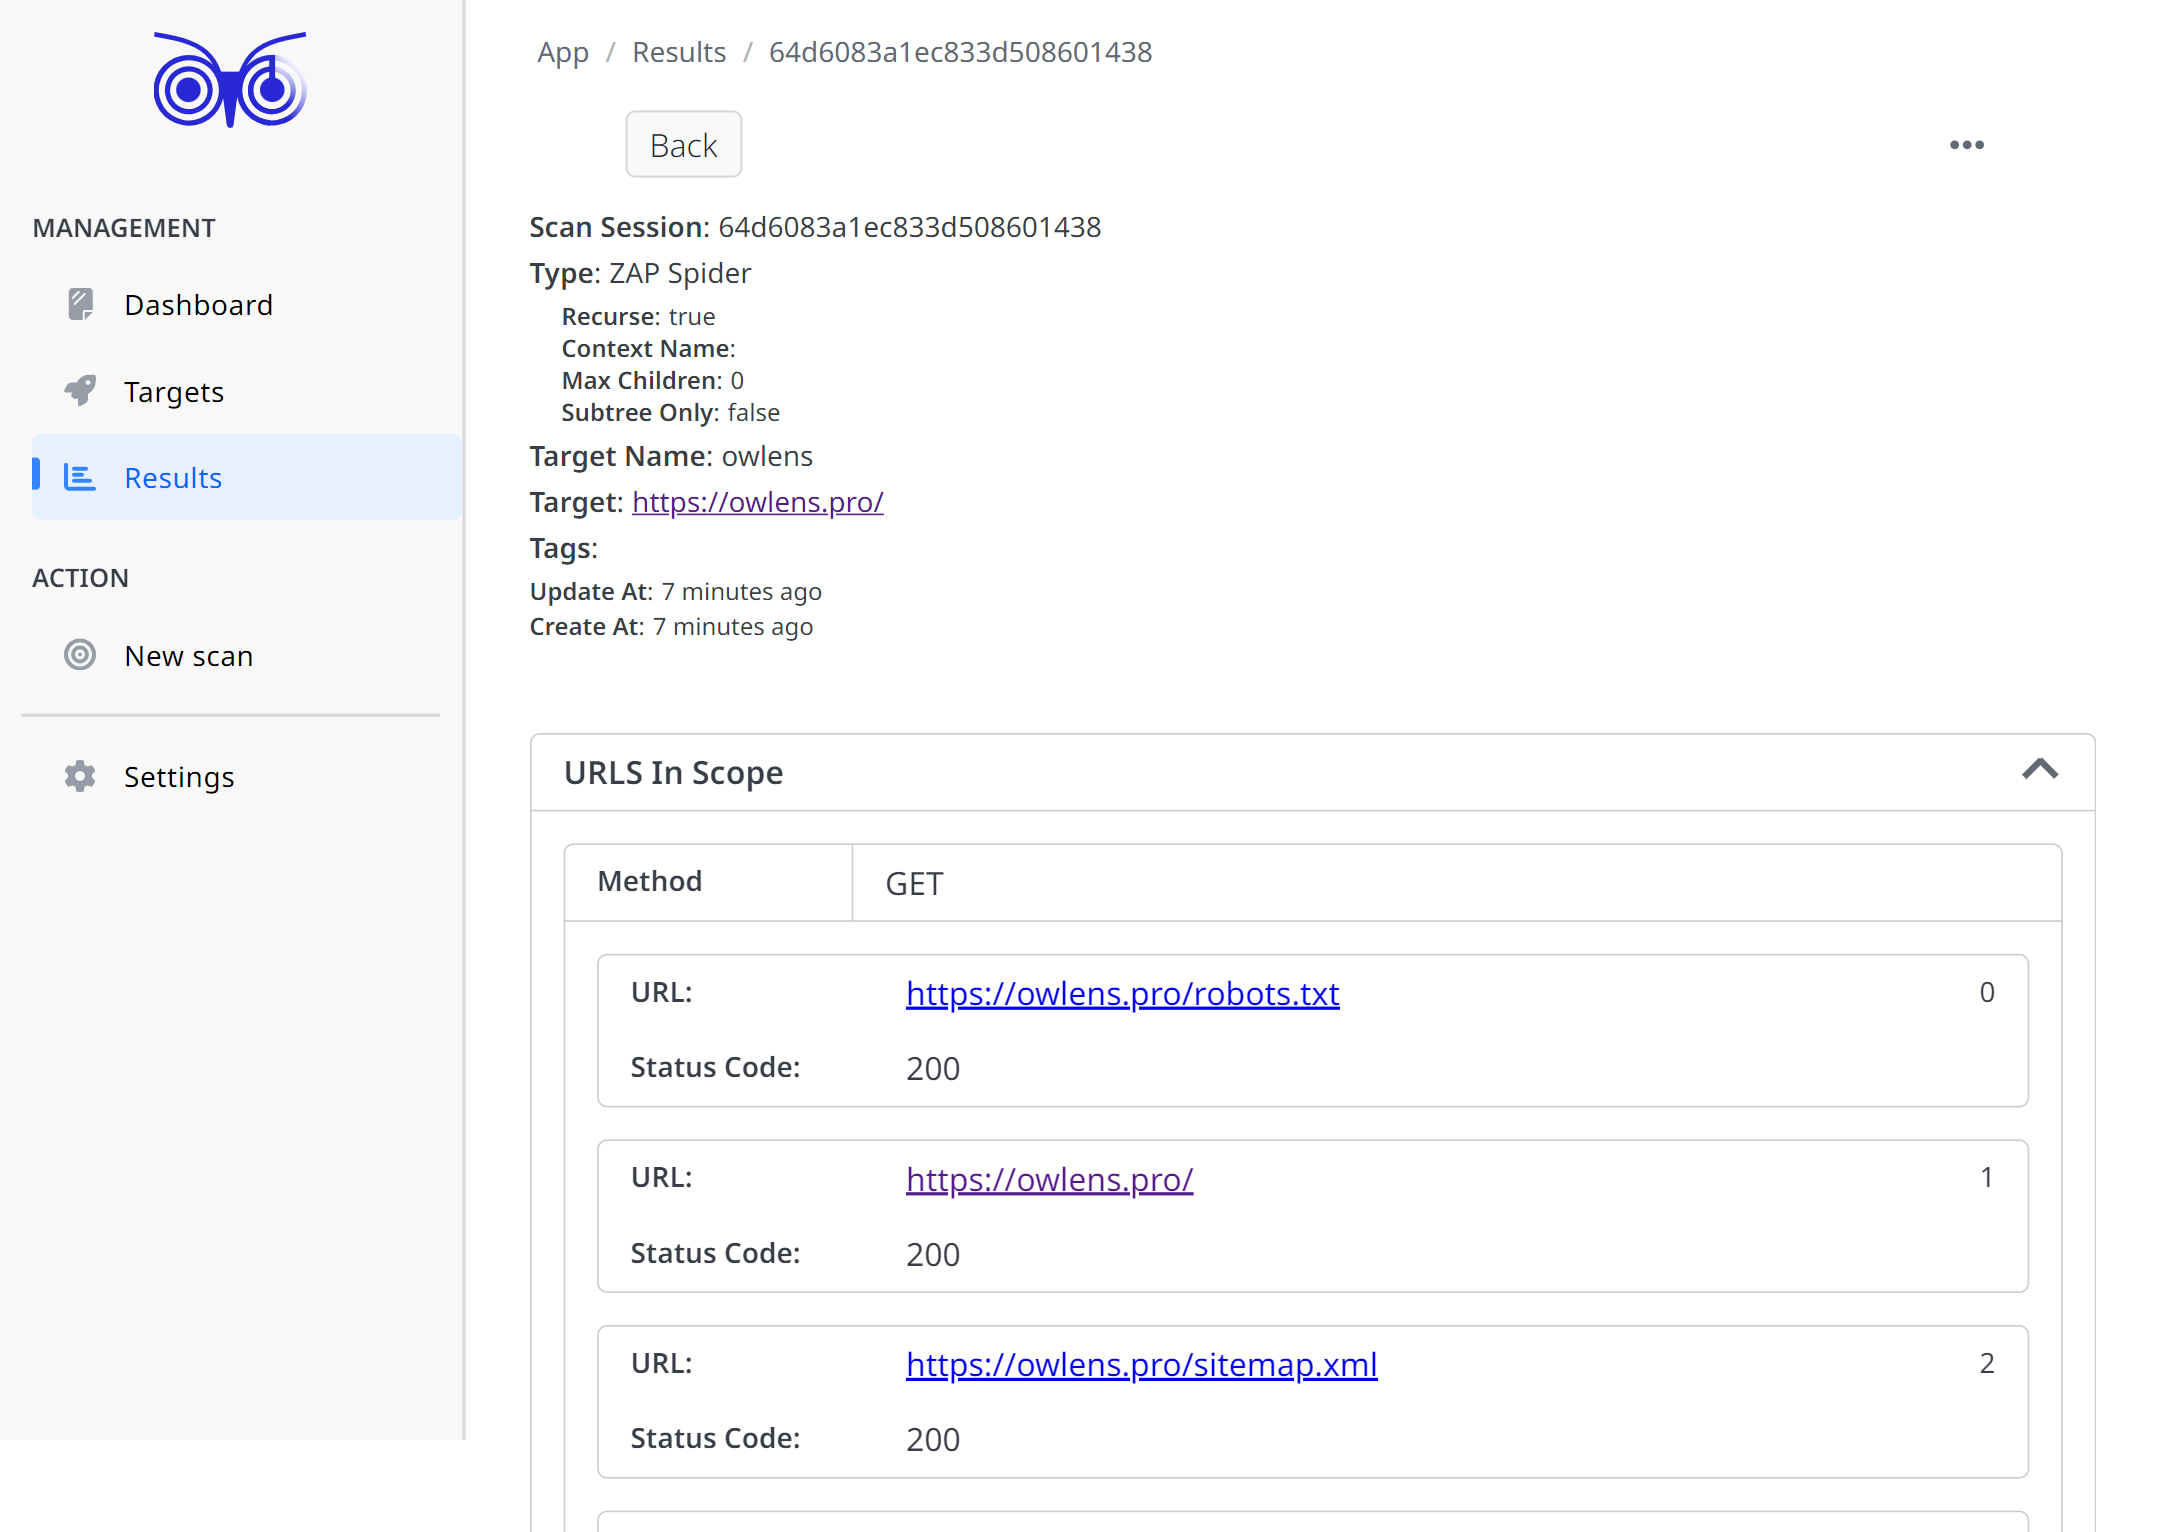
\includegraphics[width=\textwidth]{applied-thesis-chapters/chapter-6/Màn hình kết quả quét chi tiết ZAP Spider và bảng URLs In Scope.png}
      \caption{Màn hình kết quả quét chi tiết ZAP Spider và bảng URLs In Scope}
      \label{fig:ManHinhKetQuaQuetChiTietSpiderVaURLsInScope}
\end{figure}

\begin{figure}[H]
      \centering
      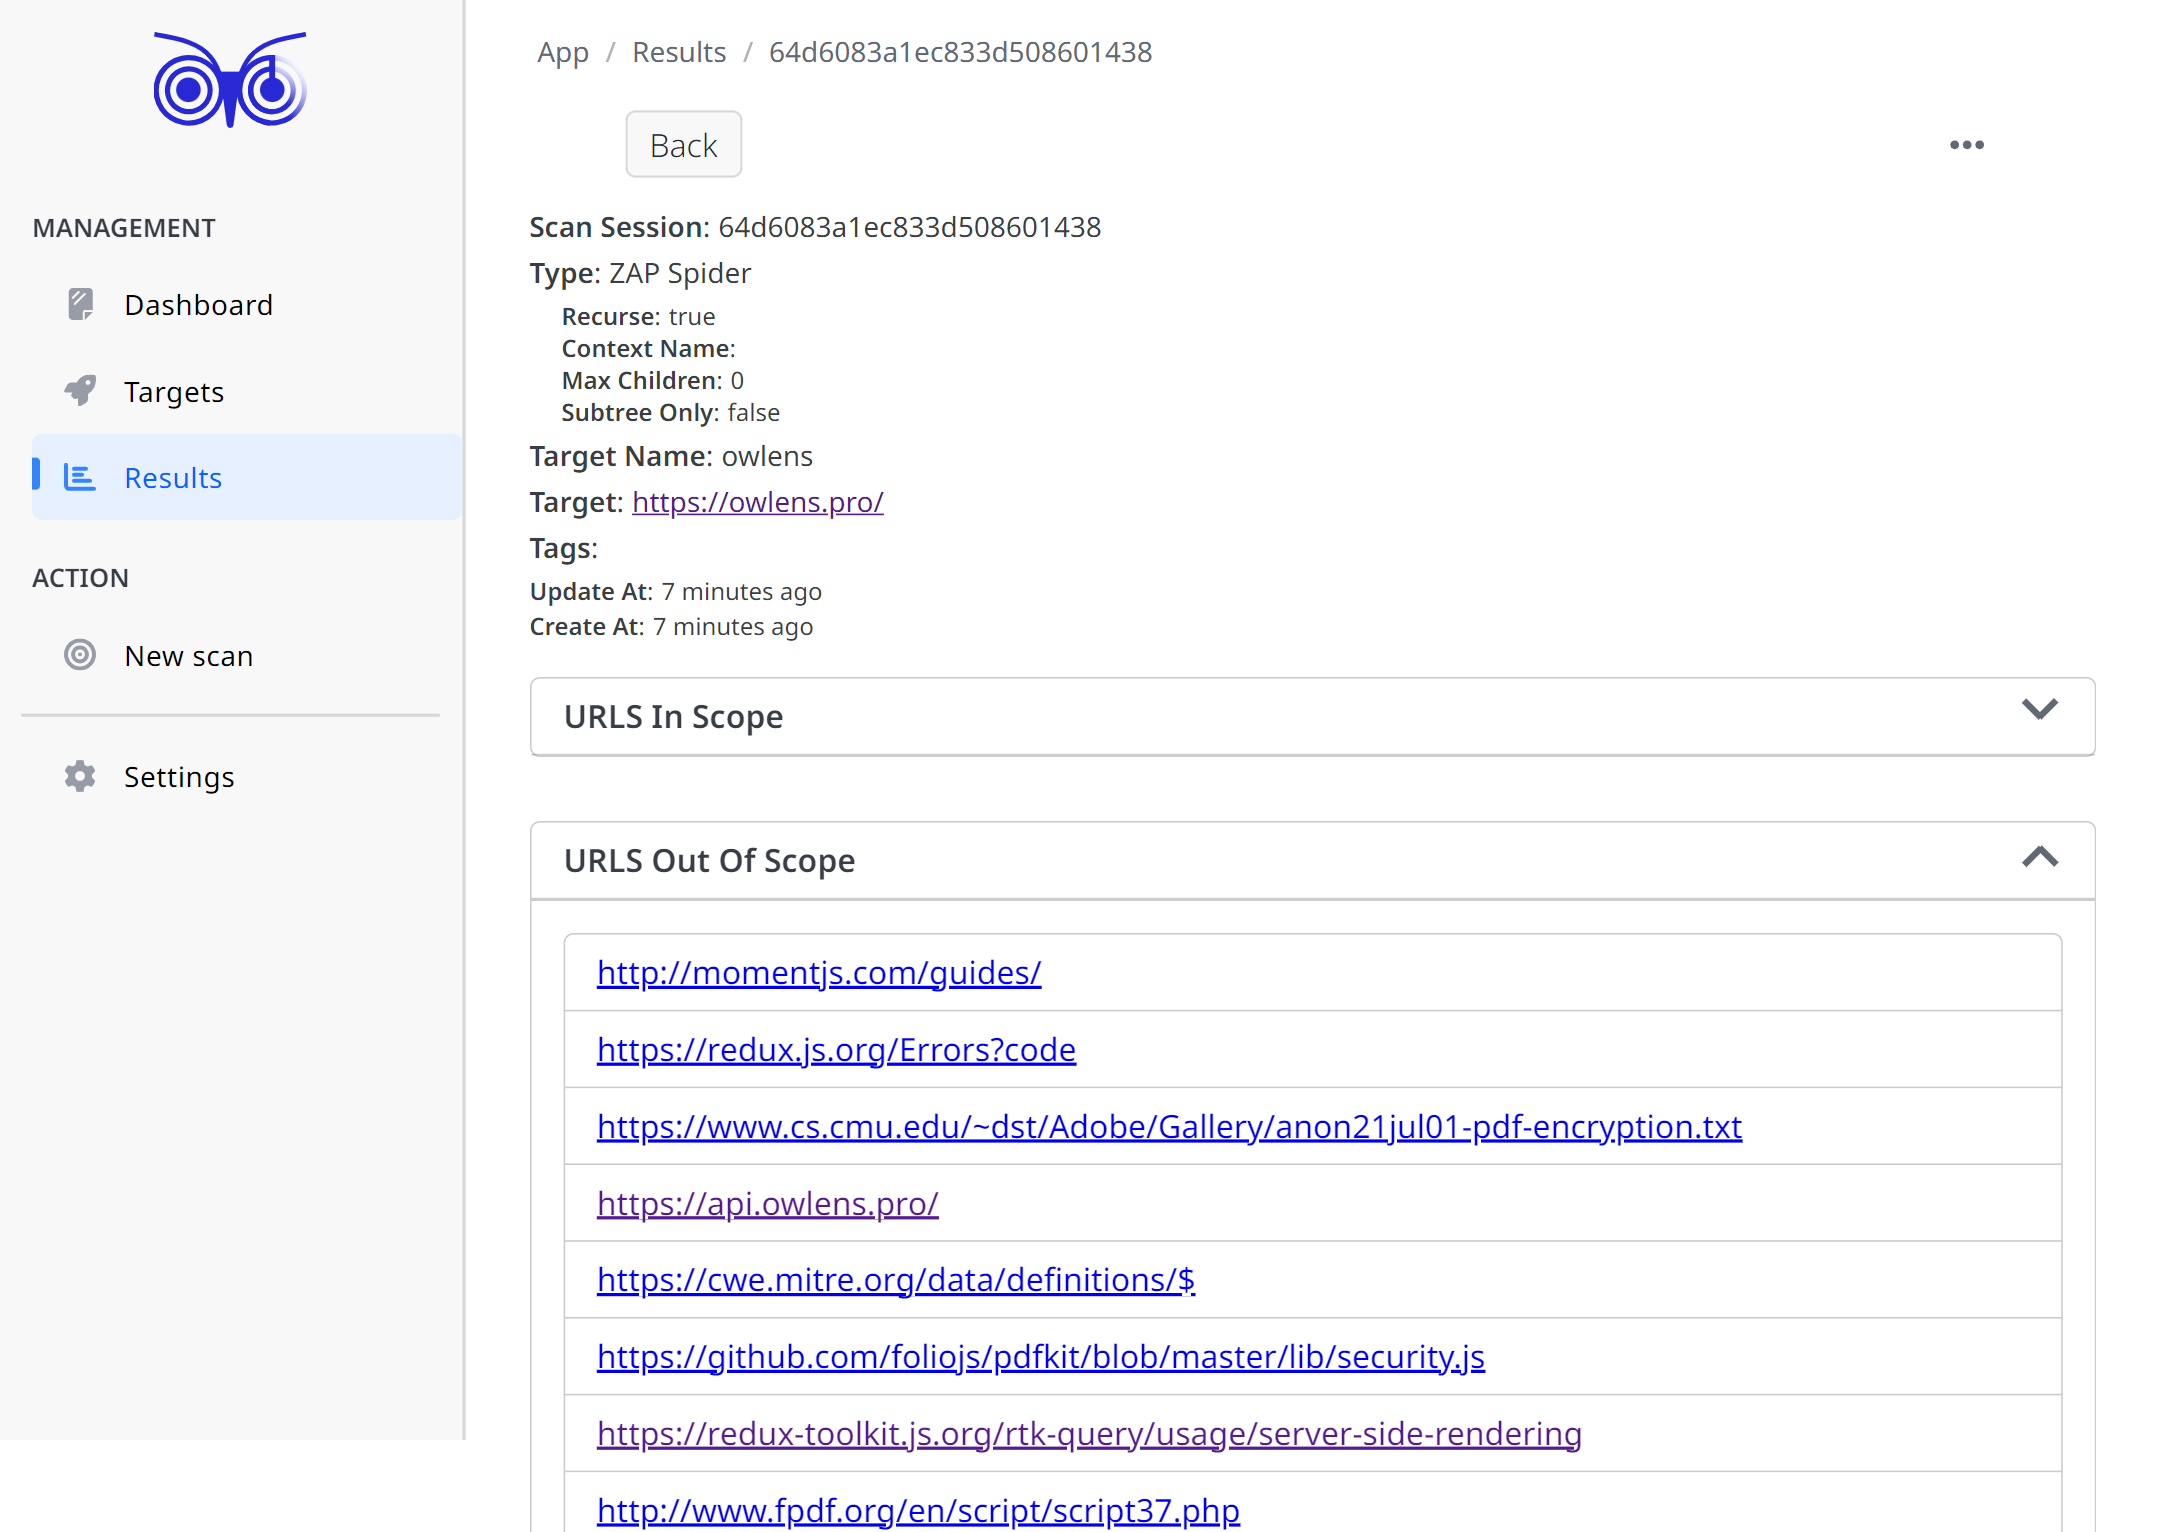
\includegraphics[width=\textwidth]{applied-thesis-chapters/chapter-6/Màn hình kết quả quét chi tiết ZAP Spider và bảng URLs Out Of Scope.png}
      \caption{Màn hình kết quả quét chi tiết ZAP Spider và bảng URLs Out Of Scope}
      \label{fig:ManHinhKetQuaQuetChiTietSpiderVaURLsOutOfScope}
\end{figure}

Các hình \textit{\ref{fig:ManHinhKetQuaQuetChiTietAjaxVaURLsInScope} \nameref{fig:ManHinhKetQuaQuetChiTietAjaxVaURLsInScope}} 
và \textit{\ref{fig:ManHinhKetQuaQuetChiTietAjaxVaURLsOutOfScope} \nameref{fig:ManHinhKetQuaQuetChiTietAjaxVaURLsOutOfScope}} 
thể hiện giao diện màn hình kết quả quét chi tiết của phiên quét loại ZAP Ajax.

\begin{figure}[H]
      \centering
      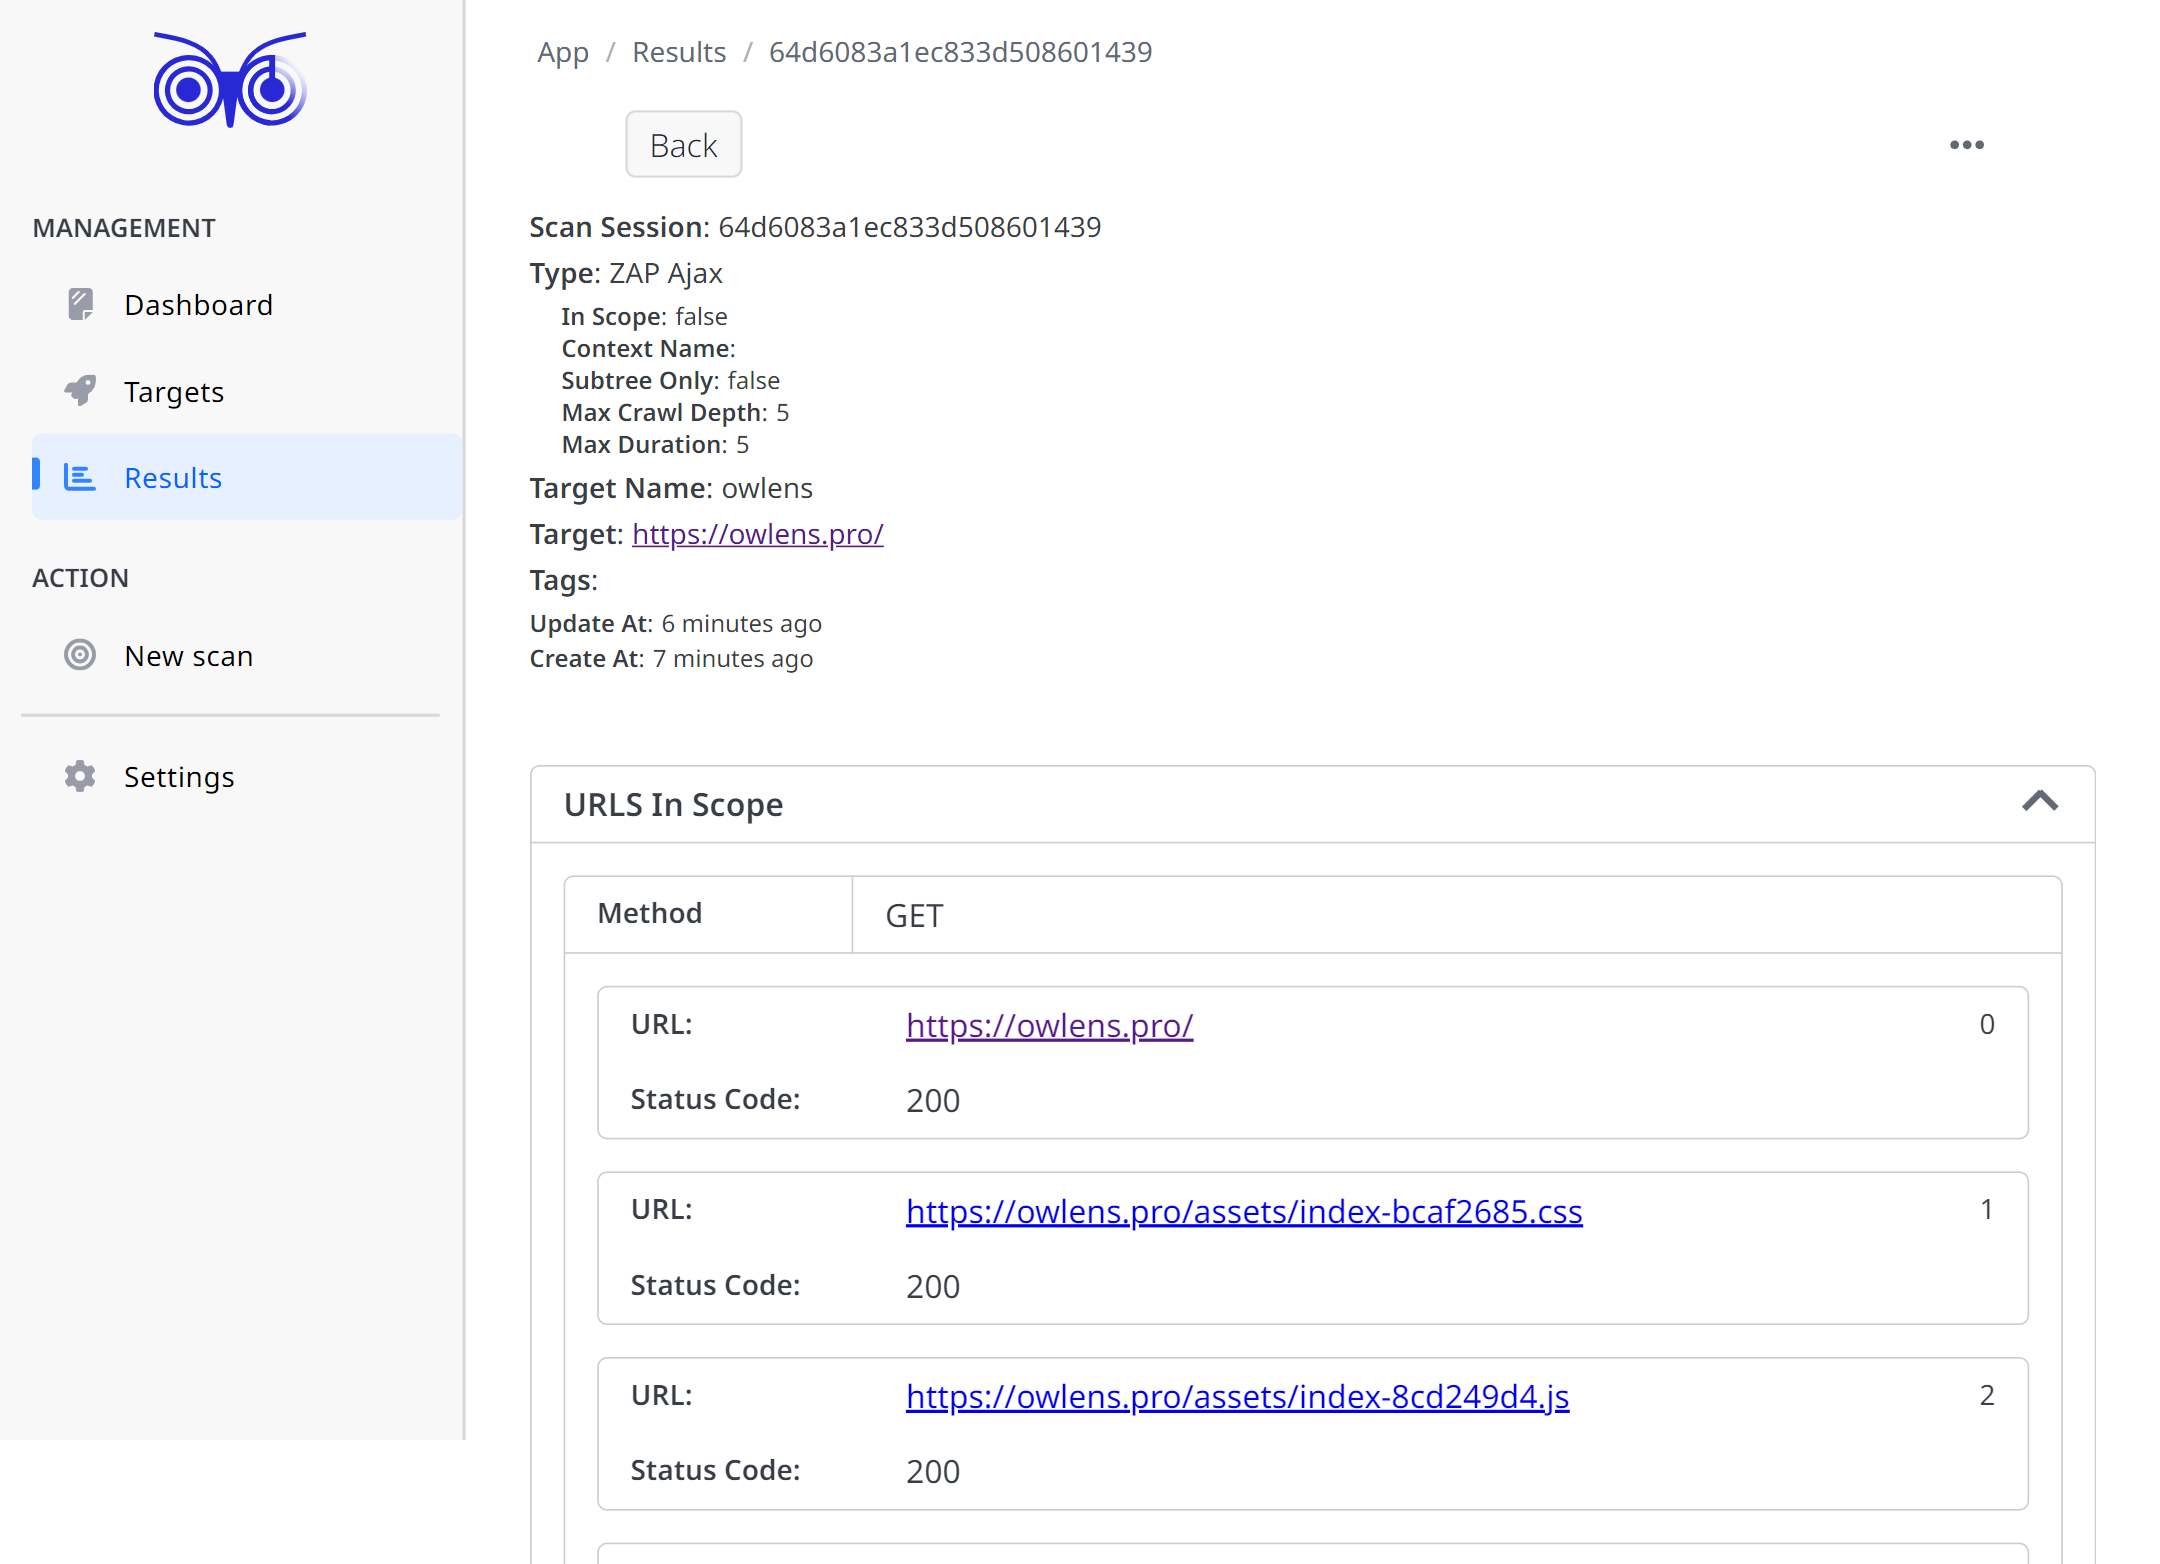
\includegraphics[width=\textwidth]{applied-thesis-chapters/chapter-6/Màn hình kết quả quét chi tiết ZAP Ajax và bảng URLs In Scope.png}
      \caption{Màn hình kết quả quét chi tiết ZAP Ajax và bảng URLs In Scope}
      \label{fig:ManHinhKetQuaQuetChiTietAjaxVaURLsInScope}
\end{figure}

\begin{figure}[H]
      \centering
      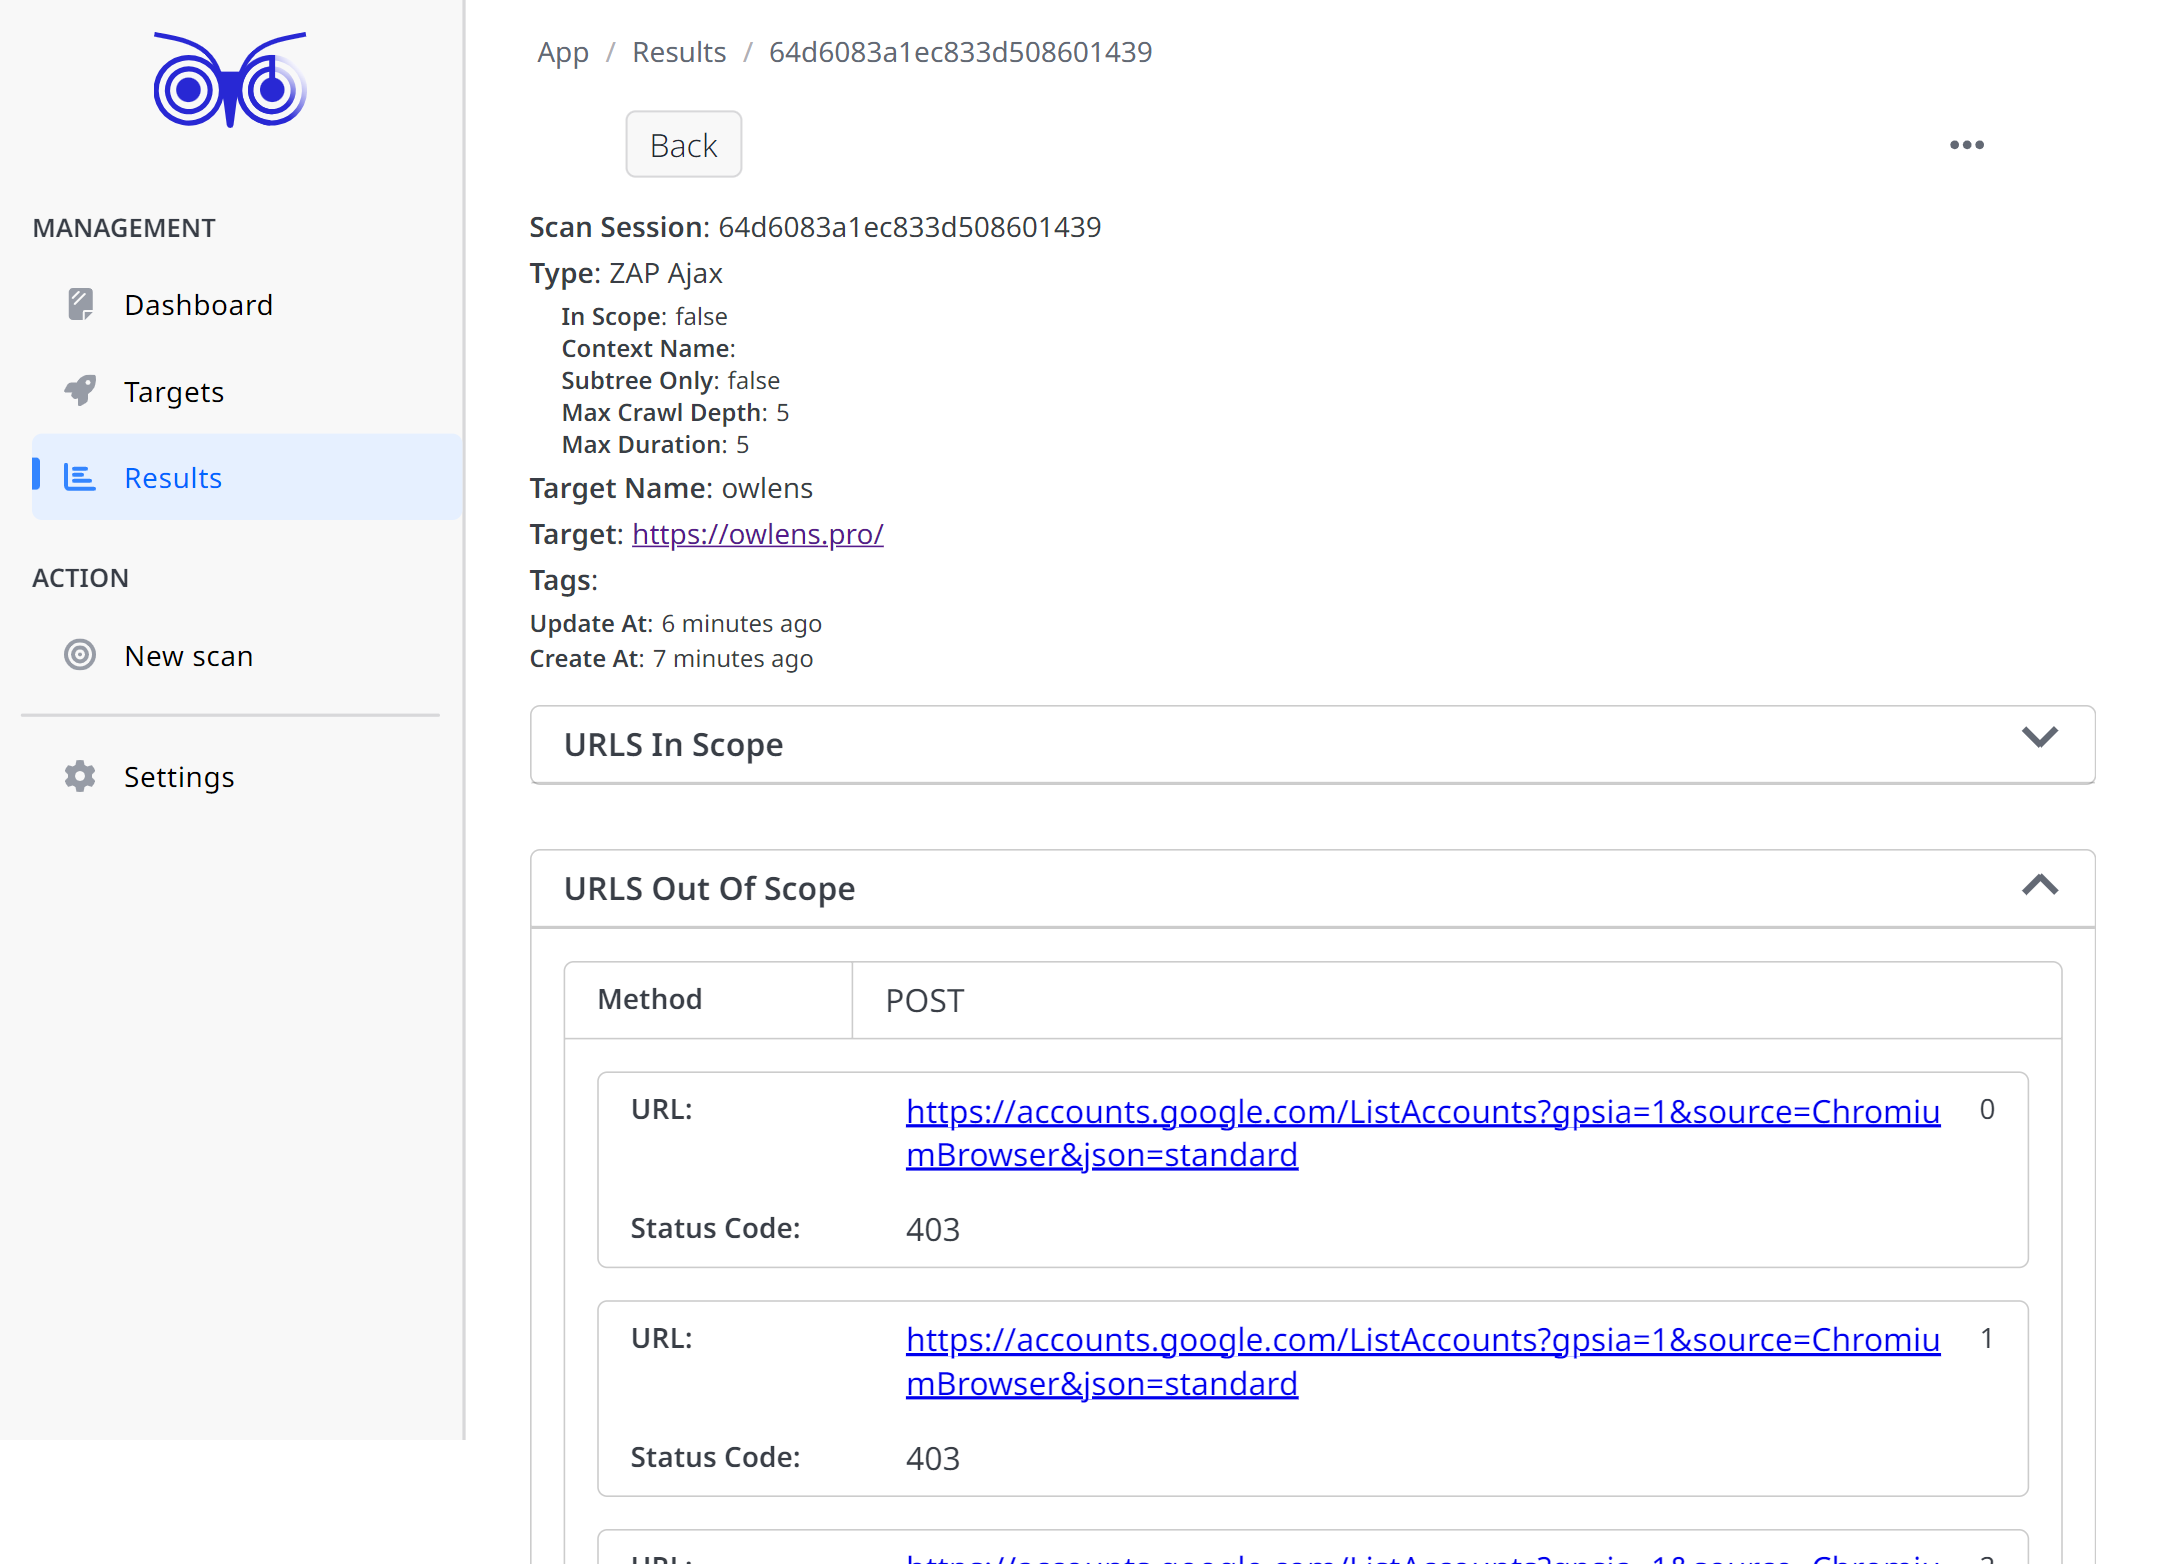
\includegraphics[width=\textwidth]{applied-thesis-chapters/chapter-6/Màn hình kết quả quét chi tiết ZAP Ajax và bảng URLs Out Of Scope.png}
      \caption{Màn hình kết quả quét chi tiết ZAP Ajax và bảng URLs Out Of Scope}
      \label{fig:ManHinhKetQuaQuetChiTietAjaxVaURLsOutOfScope}
\end{figure}

Các hình \textit{\ref{fig:ManHinhKetQuaQuetChiTietActiveVaAlertsSummary} \nameref{fig:ManHinhKetQuaQuetChiTietActiveVaAlertsSummary}}
, \textit{\ref{fig:ManHinhKetQuaQuetChiTietActiveVaAlertsInformation} \nameref{fig:ManHinhKetQuaQuetChiTietActiveVaAlertsInformation}} 
và \textit{\ref{fig:ManHinhKetQuaQuetChiTietActiveVaAlertsDetail} \nameref{fig:ManHinhKetQuaQuetChiTietActiveVaAlertsDetail}} 
thể hiện giao diện màn hình kết quả quét chi tiết của phiên quét loại ZAP Active.
Tương tự như ZAP Active, hình \textit{\ref{fig:ManHinhKetQuaQuetChiTietPassive} \nameref{fig:ManHinhKetQuaQuetChiTietPassive}} 
thể hiện cho phiên quét loại ZAP Passive.

\begin{figure}[H]
      \centering
      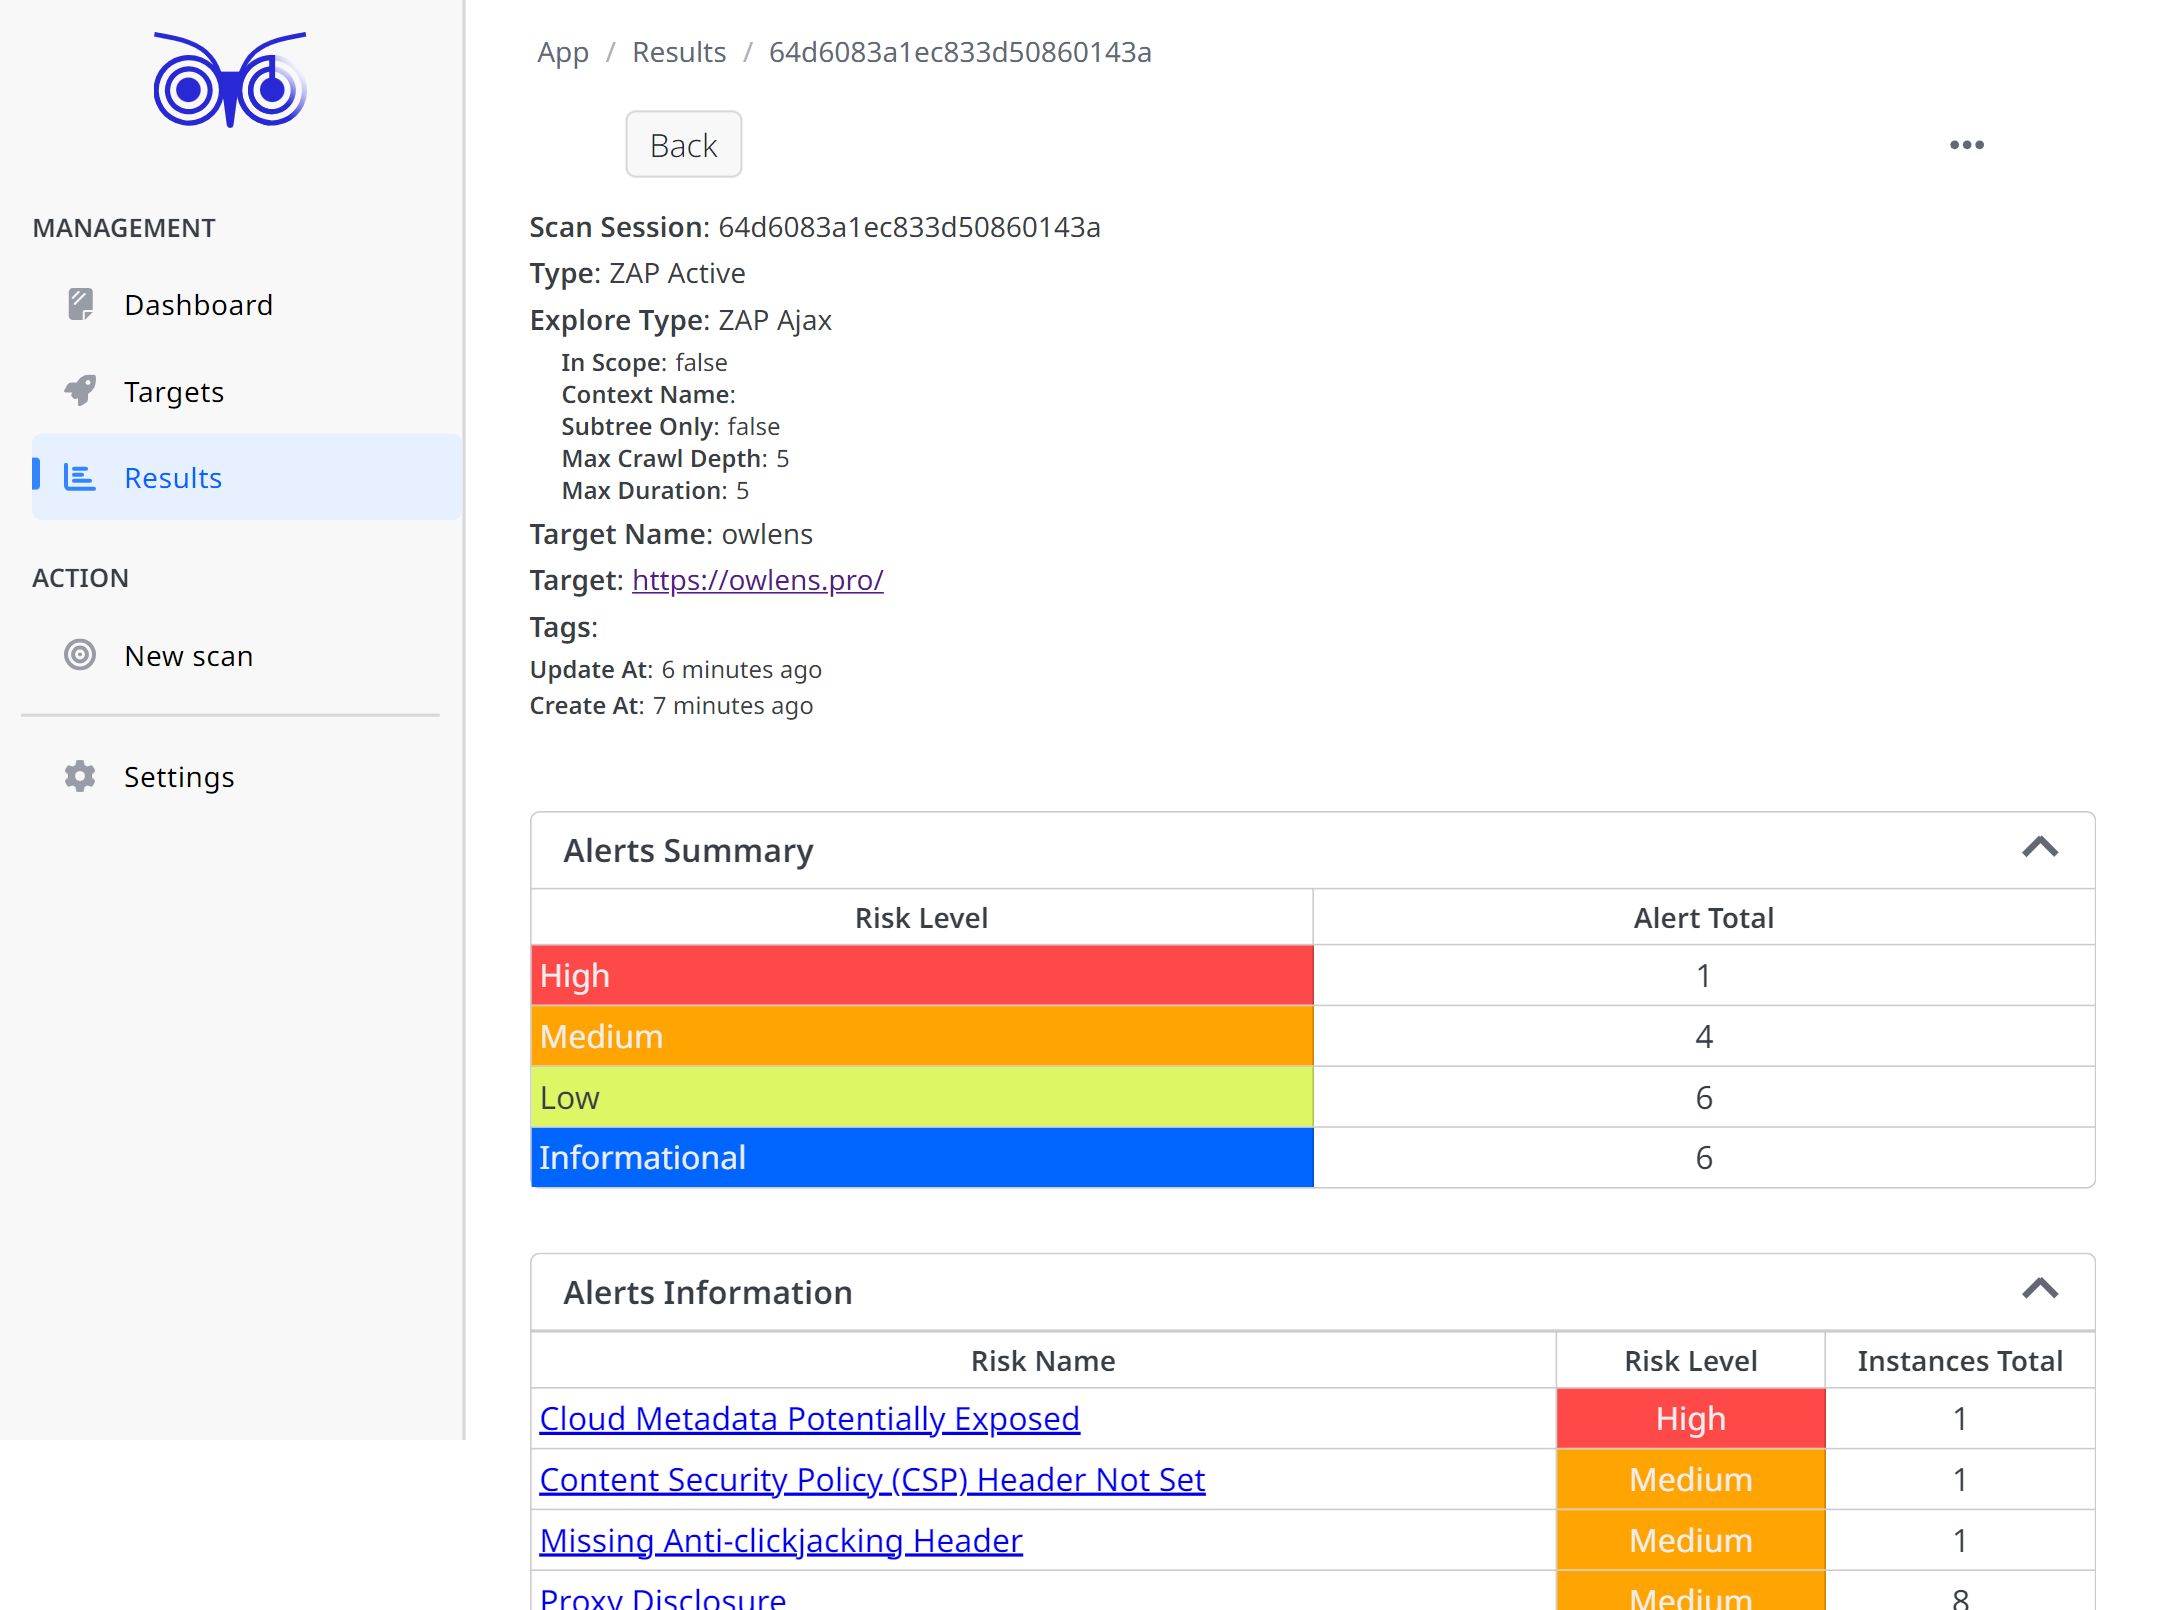
\includegraphics[width=\textwidth]{applied-thesis-chapters/chapter-6/Màn hình kết quả quét chi tiết ZAP Active và bảng Alerts Summary.png}
      \caption{Màn hình kết quả quét chi tiết ZAP Active và bảng Alerts Summary}
      \label{fig:ManHinhKetQuaQuetChiTietActiveVaAlertsSummary}
\end{figure}

\begin{figure}[H]
      \centering
      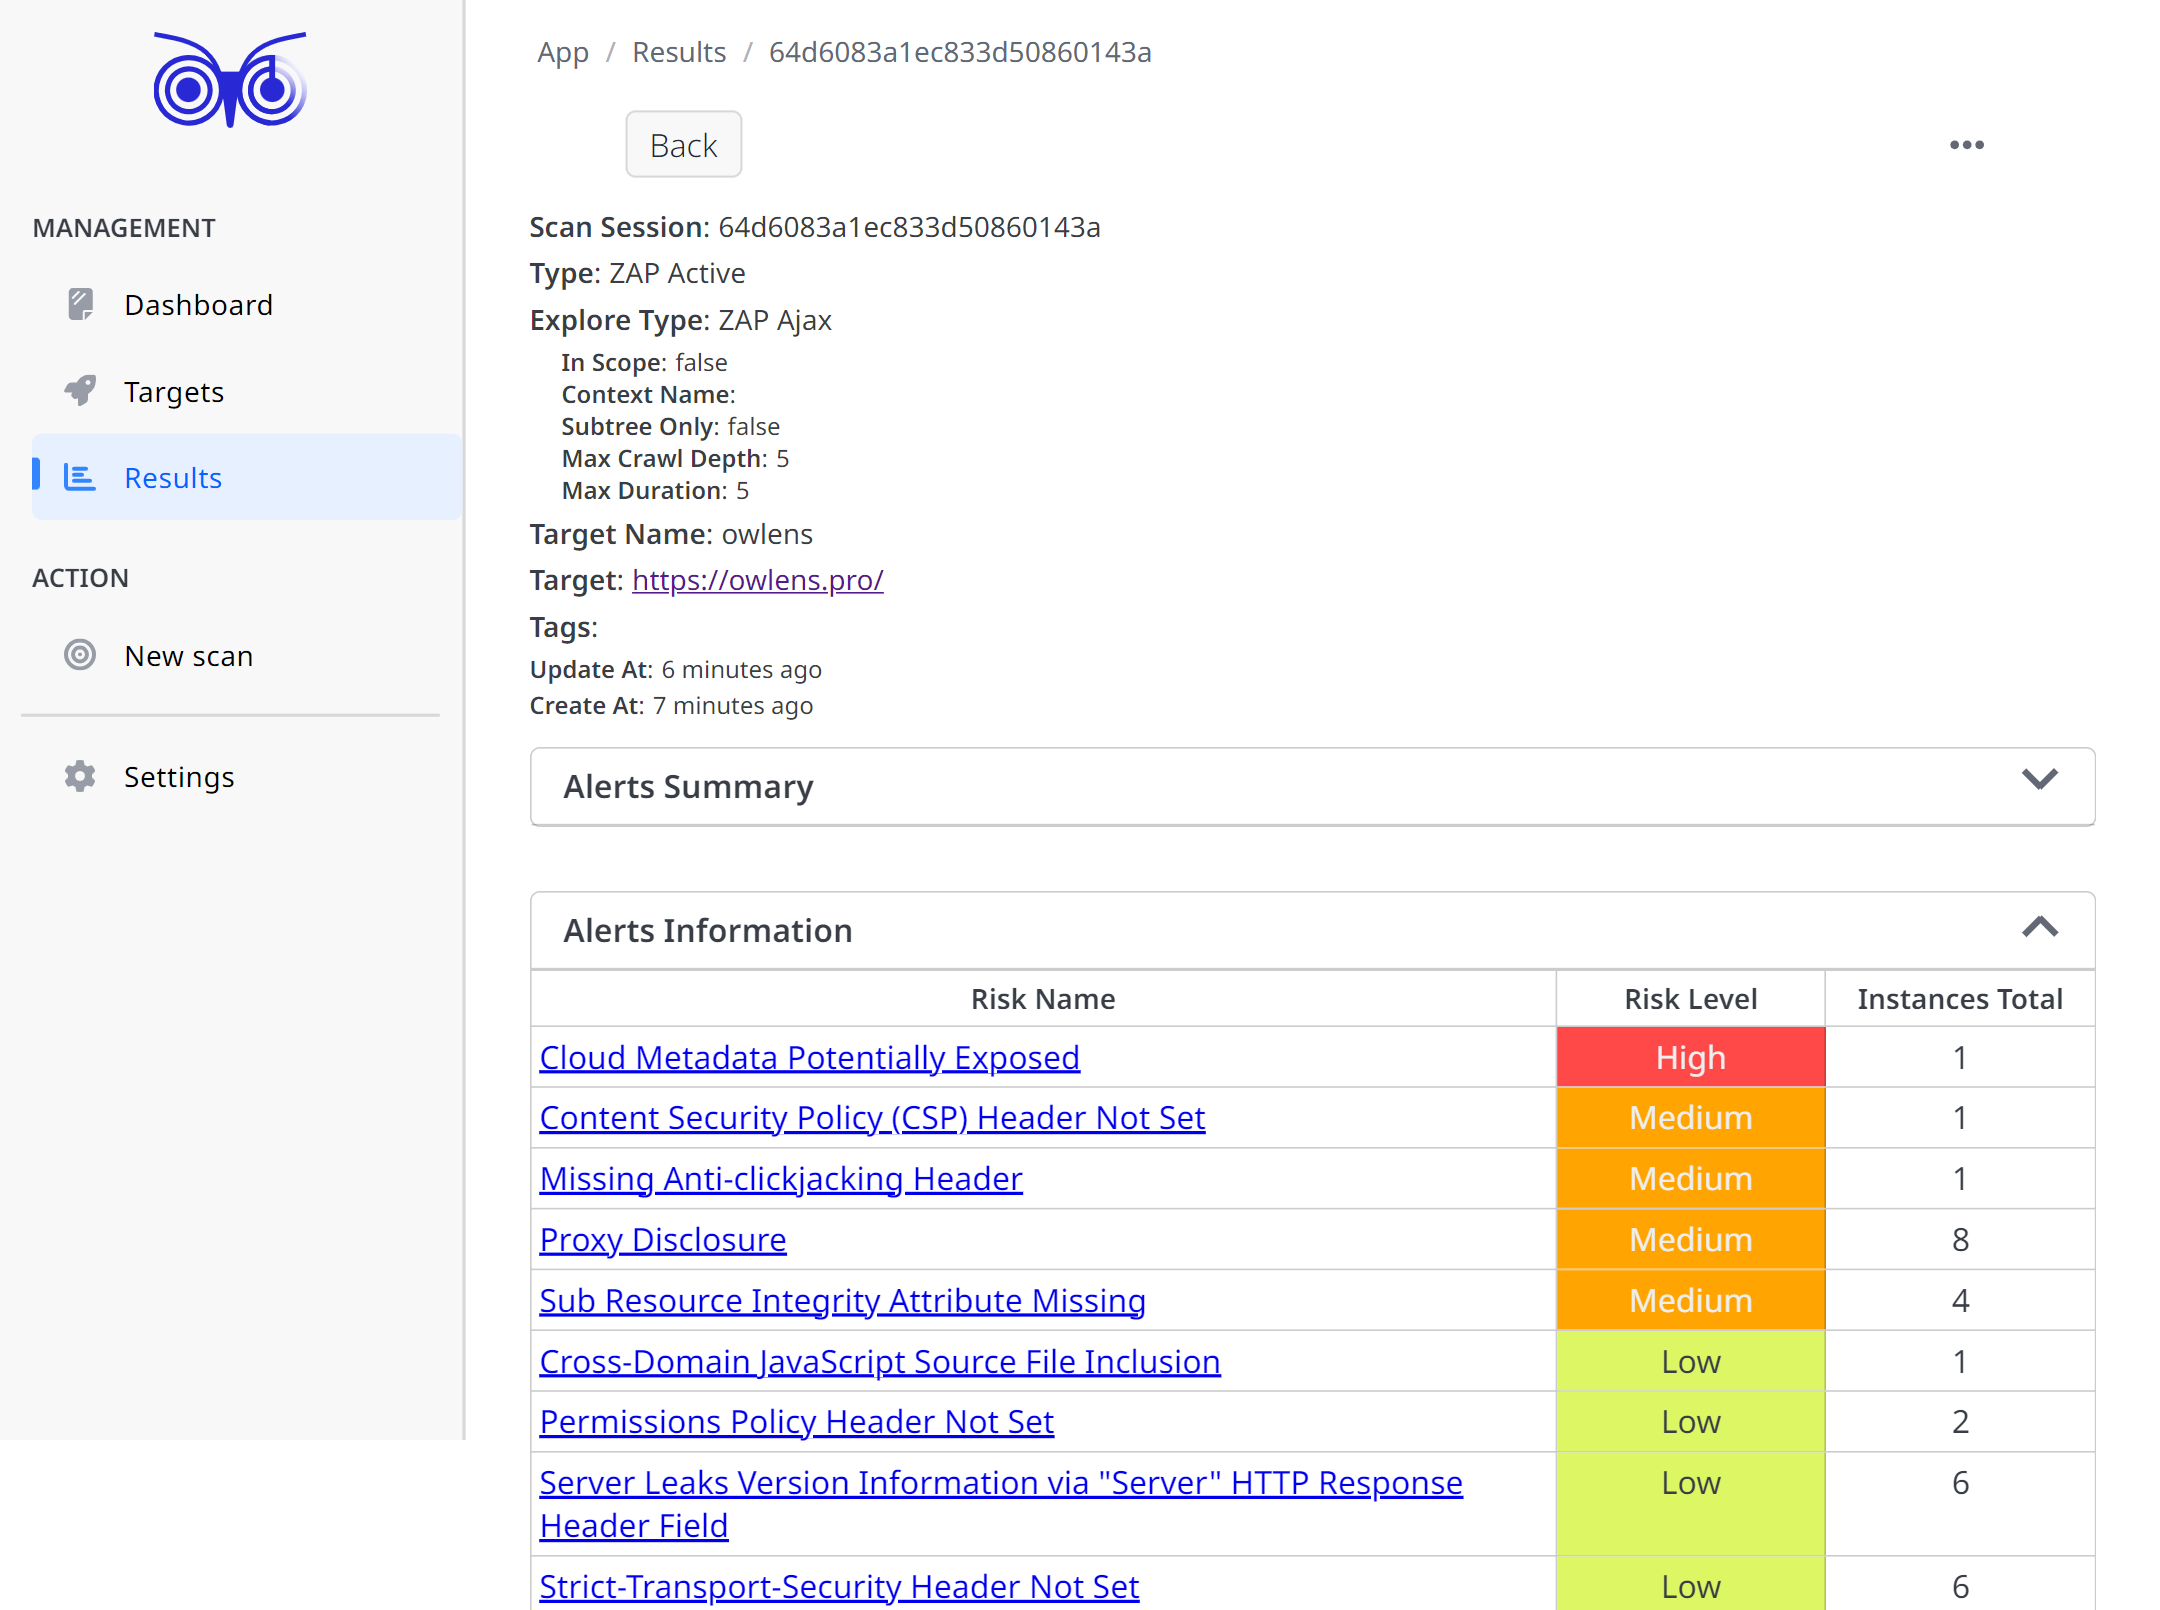
\includegraphics[width=\textwidth]{applied-thesis-chapters/chapter-6/Màn hình kết quả quét chi tiết ZAP Active và bảng Alerts Information.png}
      \caption{Màn hình kết quả quét chi tiết ZAP Active và bảng Alerts Information}
      \label{fig:ManHinhKetQuaQuetChiTietActiveVaAlertsInformation}
\end{figure}

\begin{figure}[H]
      \centering
      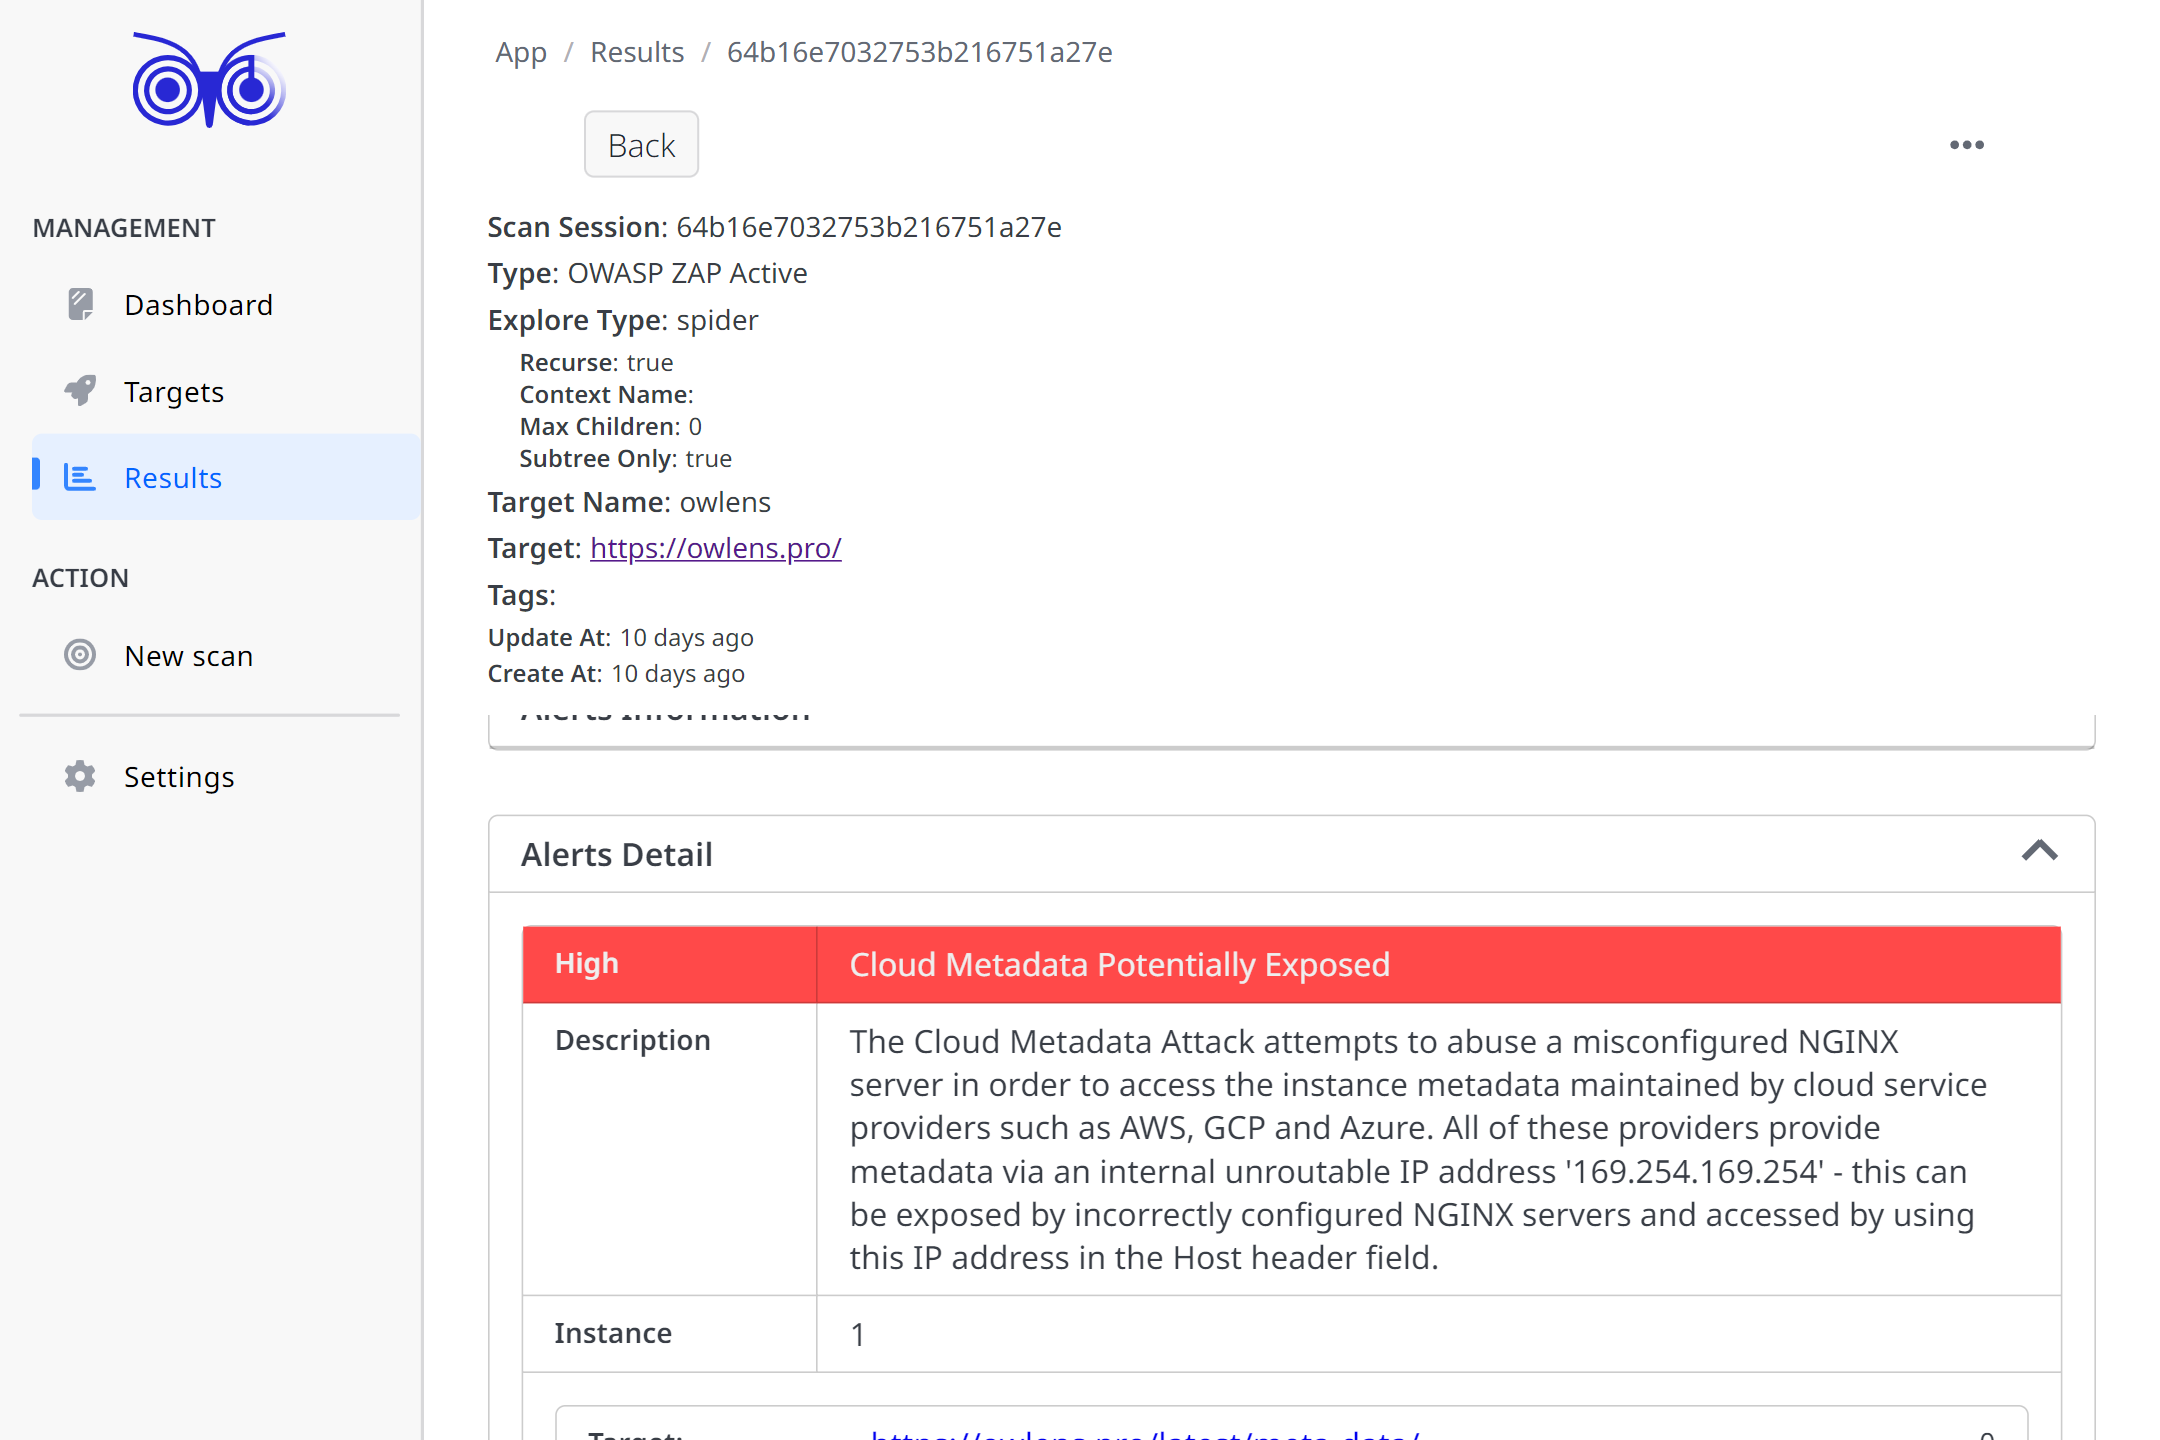
\includegraphics[width=\textwidth]{applied-thesis-chapters/chapter-6/Màn hình kết quả quét chi tiết ZAP Active và bảng Alerts Detail.png}
      \caption{Màn hình kết quả quét chi tiết ZAP Active và bảng Alerts Detail}
      \label{fig:ManHinhKetQuaQuetChiTietActiveVaAlertsDetail}
\end{figure}

\begin{figure}[H]
      \centering
      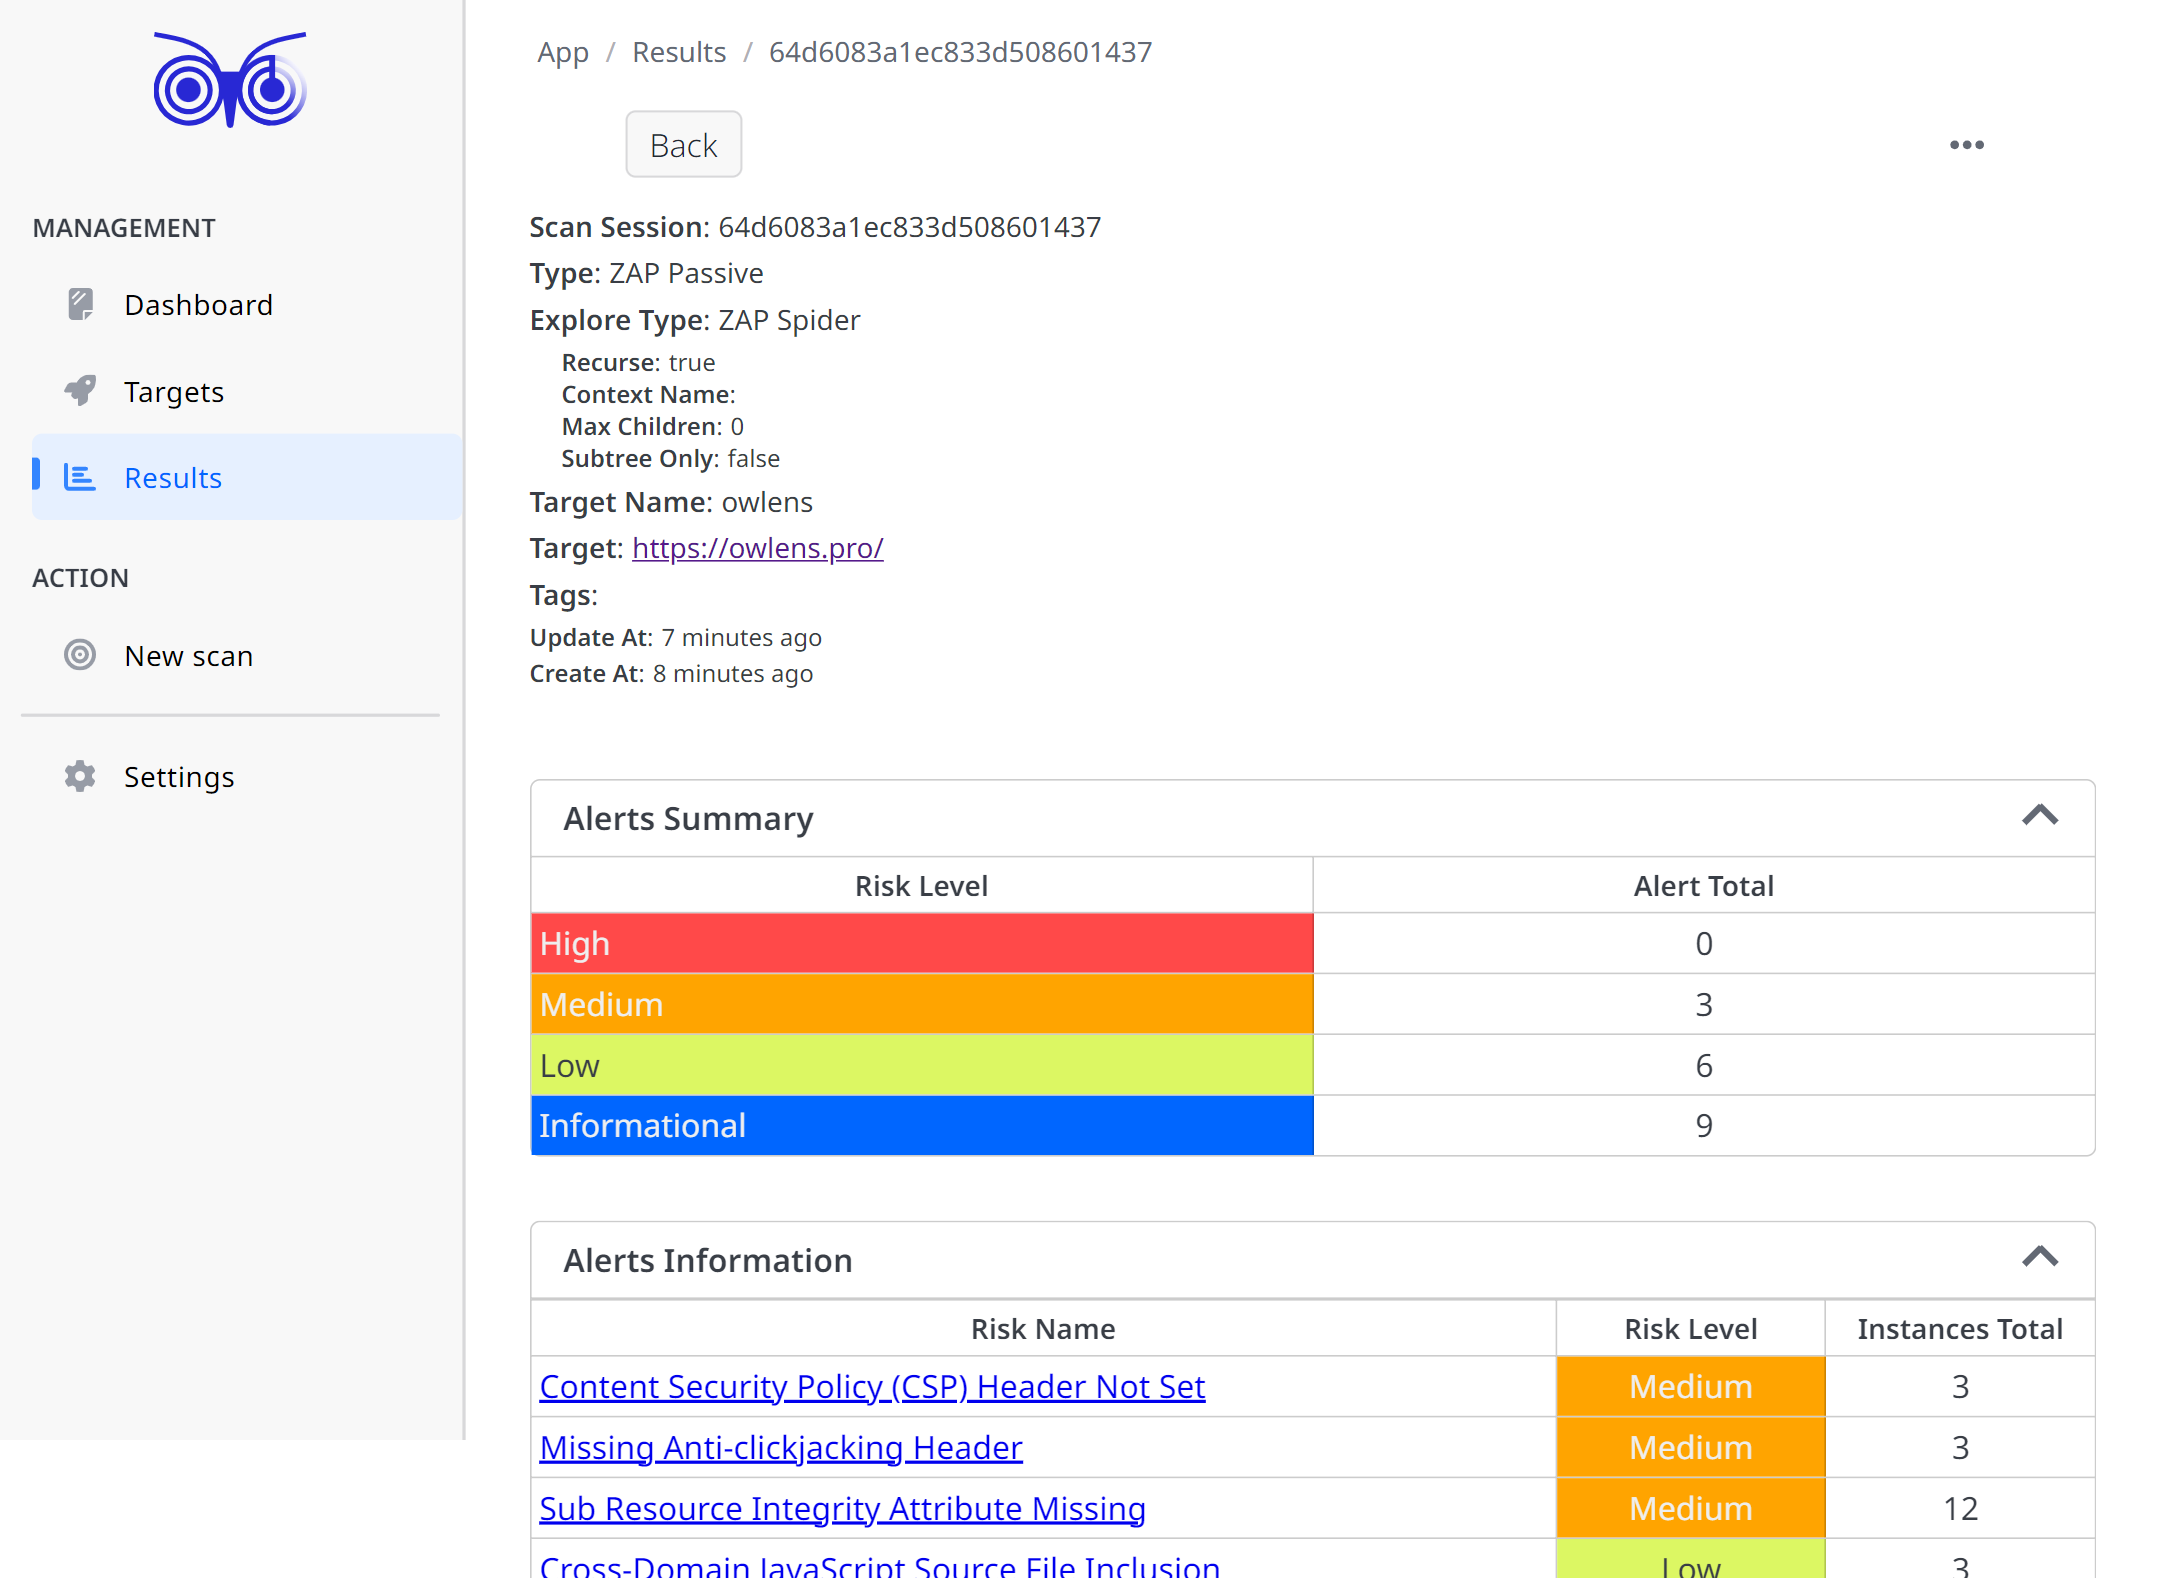
\includegraphics[width=\textwidth]{applied-thesis-chapters/chapter-6/Màn hình kết quả quét chi tiết ZAP Passive.png}
      \caption{Màn hình kết quả quét chi tiết ZAP Passive}
      \label{fig:ManHinhKetQuaQuetChiTietPassive}
\end{figure}

Như đã trình bày ở mục \textit{\ref{subsubsec:CaiDatChucNangXemKetQuaQuetChiTiet} \nameref{subsubsec:CaiDatChucNangXemKetQuaQuetChiTiet}}
, ở màn hình này, đối với ZAP Passive và ZAP Active sẽ giống nhau ở phần full result và khác nhau ở phần scan session.

\myparagraph{Tạo phiên quét (New scan)}
\tab \tab Để tạo mới một phiên quét, người dùng phải trải qua 2 bước là chọn mục tiêu và chọn cấu hình quét ở phần New scan.
Nếu người dùng chọn tạo mới phiên quét từ mục mục tiêu ở Targets thì người dùng chỉ cần chọn tiếp cấu hình quét.
Các hình \textit{\ref{fig:ManHinhNewScanVaSelectTargets} \nameref{fig:ManHinhNewScanVaSelectTargets}} 
, \textit{\ref{fig:ManHinhNewScanVaConfigureScans} \nameref{fig:ManHinhNewScanVaConfigureScans}} 
thể hiện giao diện màn hình của 2 bước này.

\begin{figure}[H]
      \centering
      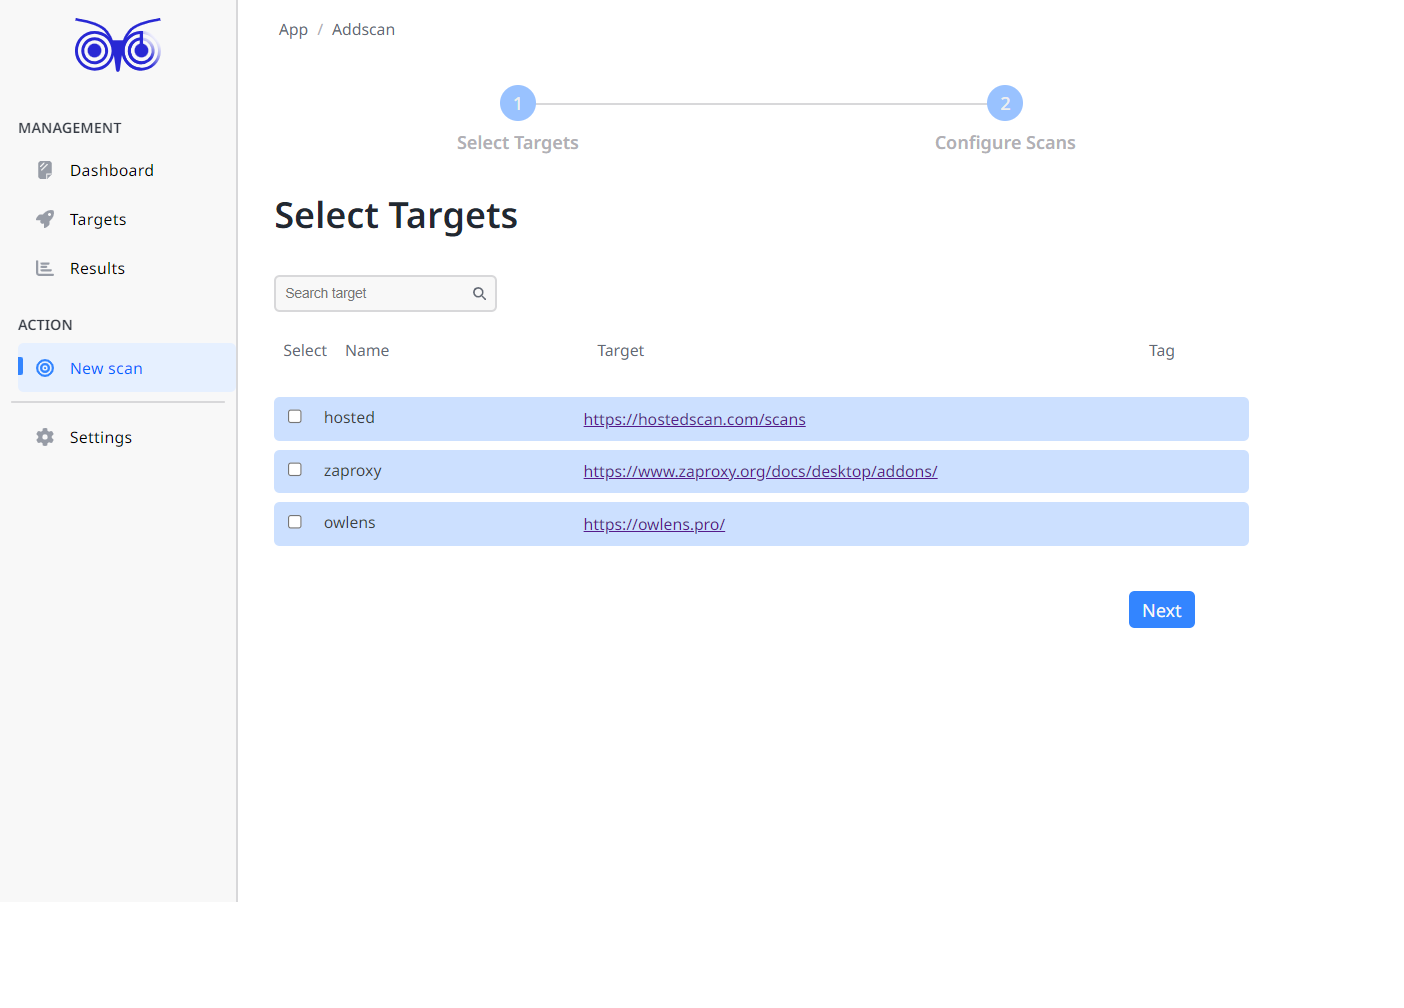
\includegraphics[width=\textwidth]{applied-thesis-chapters/chapter-6/Màn hình New Scan và bước Select Targets.png}
      \caption{Màn hình New Scan và bước Select Targets}
      \label{fig:ManHinhNewScanVaSelectTargets}
\end{figure}

\begin{figure}[H]
      \centering
      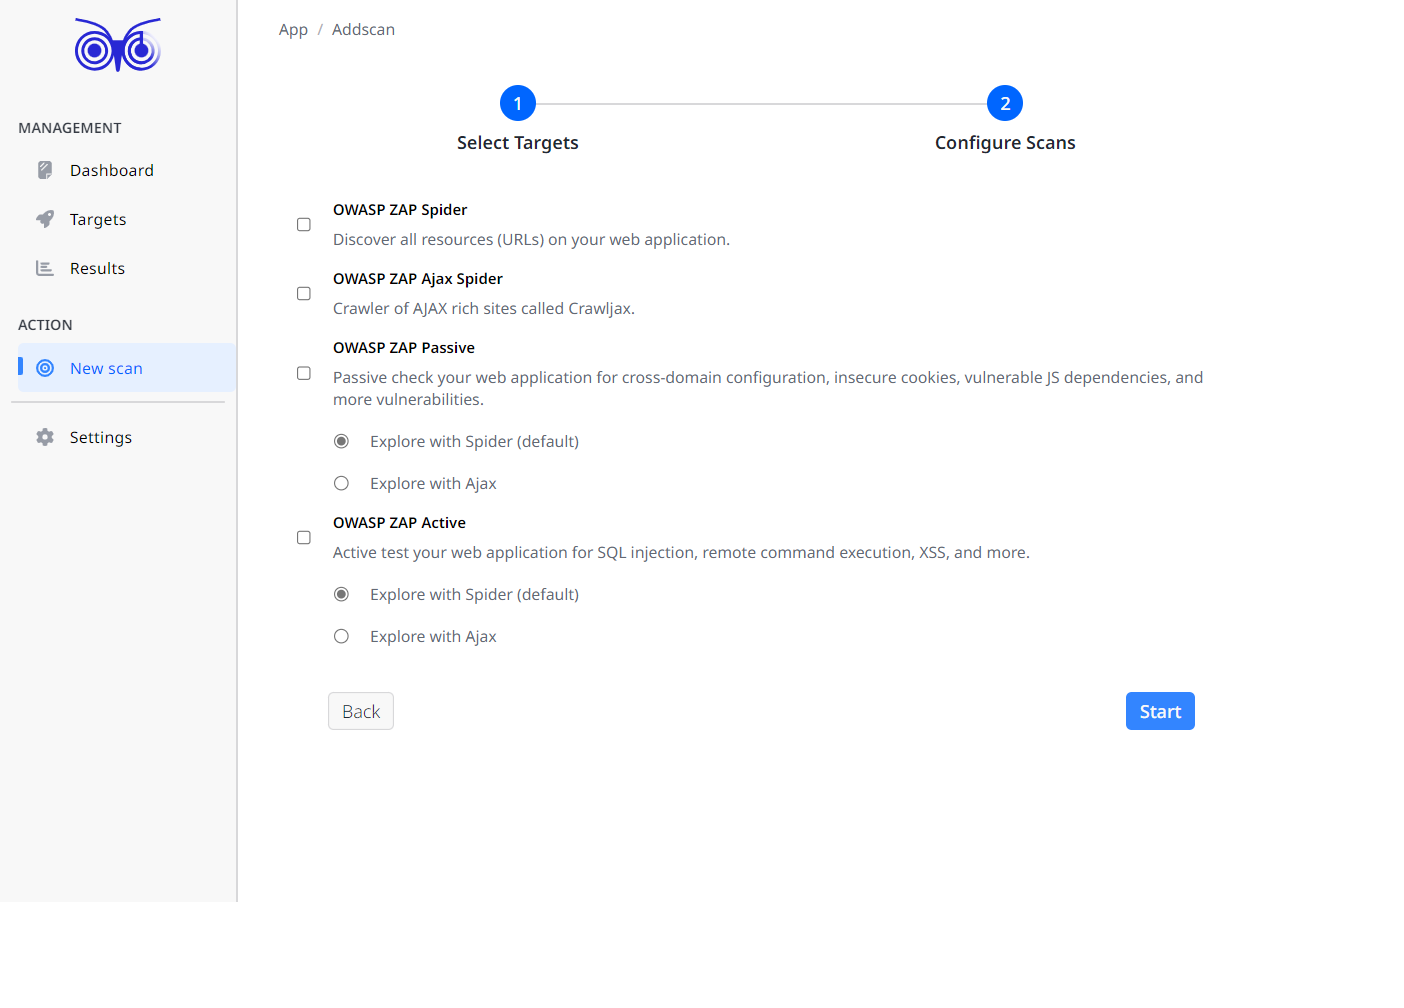
\includegraphics[width=\textwidth]{applied-thesis-chapters/chapter-6/Màn hình New Scan và bước Configure Scans.png}
      \caption{Màn hình New Scan và bước Configure Scans}
      \label{fig:ManHinhNewScanVaConfigureScans}
\end{figure}

\myparagraph{Cài đặt (Settings)}
\tab \tab Hình \textit{\ref{fig:ManHinhSettings} \nameref{fig:ManHinhSettings}} thể hiện giao diện màn hình phần Settings.

\begin{figure}[H]
      \centering
      \includegraphics[width=\textwidth]{applied-thesis-chapters/chapter-6/Màn hình Settings.png}
      \caption{Màn hình Settings}
      \label{fig:ManHinhSettings}
\end{figure}

Màn hình hiển thị hình ảnh, tên và thông email mà người dùng đã dùng để đăng nhập.
Đồng thời người dùng cũng thực hiện đăng xuất khỏi ứng dụng ở màn hình này.

\subsection{Cấu trúc nội dung các tệp báo cáo}

\tab Ở màn hình kết quả quét chi tiết, người dùng có thể xuất tệp PDF báo cáo chi tiết cho kết quả quét.
Như đã nhắc đến ở mục \textit{\ref{subsubsec:CaiDatChucNangXuatTepPDF} \nameref{subsubsec:CaiDatChucNangXuatTepPDF}}, 
các loại báo cáo khác nhau sẽ có cách trình bày thông tin khác nhau.

Các hình \textit{\ref{fig:SoLuocCauTrucNoiDungBaoCaoZapSpider} \nameref{fig:SoLuocCauTrucNoiDungBaoCaoZapSpider}}
, \textit{\ref{fig:SoLuocCauTrucNoiDungBaoCaoZapAjax} \nameref{fig:SoLuocCauTrucNoiDungBaoCaoZapAjax}}
, \textit{\ref{fig:SoLuocCauTrucNoiDungBaoCaoZapPassive} \nameref{fig:SoLuocCauTrucNoiDungBaoCaoZapPassive}}
và \textit{\ref{fig:SoLuocCauTrucNoiDungBaoCaoZapActive} \nameref{fig:SoLuocCauTrucNoiDungBaoCaoZapActive}} 
thể hiện sơ lược cấu trúc thông tin được trình bày trong các tệp báo cáo.

\begin{figure}[H]
      \centering
      \includegraphics[width=\textwidth]{applied-thesis-chapters/chapter-6/Sơ lược cấu trúc nội dung báo cáo ZAP Spider.png}
      \caption{Sơ lược cấu trúc nội dung báo cáo ZAP Spider}
      \label{fig:SoLuocCauTrucNoiDungBaoCaoZapSpider}
\end{figure}

\begin{figure}[H]
      \centering
      \includegraphics[width=\textwidth]{applied-thesis-chapters/chapter-6/Sơ lược cấu trúc nội dung báo cáo ZAP Ajax.png}
      \caption{Sơ lược cấu trúc nội dung báo cáo ZAP Ajax}
      \label{fig:SoLuocCauTrucNoiDungBaoCaoZapAjax}
\end{figure}

\begin{figure}[H]
      \centering
      \includegraphics[width=\textwidth]{applied-thesis-chapters/chapter-6/Sơ lược cấu trúc nội dung báo cáo ZAP Passive.png}
      \caption{Sơ lược cấu trúc nội dung báo cáo ZAP Passive}
      \label{fig:SoLuocCauTrucNoiDungBaoCaoZapPassive}
\end{figure}

\begin{figure}[H]
      \centering
      \includegraphics[width=\textwidth]{applied-thesis-chapters/chapter-6/Sơ lược cấu trúc nội dung báo cáo ZAP Active.png}
      \caption{Sơ lược cấu trúc nội dung báo cáo ZAP Active}
      \label{fig:SoLuocCauTrucNoiDungBaoCaoZapActive}
\end{figure}

\newpage
\printbibliography[title={Tài liệu tham khảo}]
\end{document}